\documentclass[twosided, 12pt, draft]{book} %twosided is nice requires (sometimes) introduces blank pagestyle, which is cool because it looks nice and lets me make fancy headers
\usepackage{emptypage} % should remove blank page headers and footers, i.e., works beautifully
\usepackage{titlesec} % modify title and section(<-doesn't work?)
\usepackage{amsmath} % lots of math functions
\usepackage{epigraph} % lets me write an epigraph obviously...
\usepackage[super]{nth} % pretty formatting of ordinal numerals
\usepackage{graphicx} % putting in figures, if one might ask..
\usepackage{braket} % Dirac notation
\usepackage{geometry}
\geometry{
    margin = 1in  % give 1in margins
}
\usepackage[font = small]{caption}
\usepackage{verbatim}
\usepackage{appendix}
\usepackage{adjustbox} % adjust figures
\usepackage{tabularx}
\usepackage{indentfirst}
\usepackage[utf8]{inputenc}
\usepackage[english]{babel}
\usepackage{amssymb} % AMS symbol package
\usepackage{amsthm}  % AMS symbol package
\newtheorem{theorem}{Theorem}[section]
\newtheorem{corollary}{Corollary}[theorem]
\newtheorem{lemma}[theorem]{Lemma}
\usepackage[toc]{glossaries} % makeglossaries thesis
\usepackage{afterpage} % very useful for formating...
\usepackage{setspace}
\doublespacing % double spaces whole document except for captions
\usepackage{notoccite}
\usepackage[symbol]{footmisc} % for footnotes with weird characters
\usepackage{afterpage} % needed this for putting things back on track, outlined below
\usepackage{textcomp}
\usepackage{fancyhdr} % allows for fancy headers
\pagestyle{fancy} % uses fancy page styling for headers and such --> change to "plain" if have to get rid of headers
\usepackage{mathtools} % for making NR= sign
\usepackage{upgreek} % for non-italicized Greek letters
\usepackage{pgffor}
\usepackage{float}

\interfootnotelinepenalty=1000 % To make sure footnotes don't get split on a separate page, 10000 is max

\setlength{\textfloatsep}{15pt} % might fix gap between text and figures, and it does!
\setlength{\parskip}{0pt} % might fix gap between paragraphs, and it does!
% now there are some weird gaps between section headings and text

\renewcommand{\chaptermark}[1]{\markboth{#1}{}} %still don't understand how this grabs chapterName but it does...
\renewcommand{\sectionmark}[1]{\markright{#1}} %still don't understand how this grabs sectionName but it does...
\fancyhead{} %clears the fancy header
\fancyhead[LO]{\MakeUppercase{\leftmark}} %Left even header for just saying chaptername

% code below lets me add a blankpage with \afterpage{\blankpage}
\newcommand\blankpage{%
    \null
    \thispagestyle{empty}%
    \addtocounter{page}{-1}%
\newpage}

  % lets me change the type of footnote
\renewcommand{\thefootnote}{\fnsymbol{footnote}}
%\allsectionsfont{\singlespacing} 

% defines shortcuts for common physics symbols
\newcommand{\tot}{\ensuremath{\sigma_{tot}}}
\newcommand{\tots}{\ensuremath{\sigma_{tot}}\,\,}
\newcommand{\totE}{\ensuremath{\sigma_{tot}}(E)}
\newcommand{\totEs}{\ensuremath{\sigma_{tot}}(E)\,\,}
\newcommand{\totRDs}{\ensuremath{\sigma_{A,A'}}(E)\,}
\newcommand{\rxn}{\ensuremath{\sigma_{rxn}}}
\newcommand{\rxnE}{\ensuremath{\sigma_{rxn}}(E)}
\newcommand{\rxnEs}{\ensuremath{\sigma_{rxn}}(E)\,\,}
\newcommand{\el}{\ensuremath{\frac{d\sigma}{d\Omega}}\,}

\newcommand{\oSix}{\ensuremath{^{16}}O}
\newcommand{\oEight}{\ensuremath{^{18}}O}
\newcommand{\neEight}{\ensuremath{^{18}}O}
\newcommand{\caForty}{\ensuremath{^{40}}Ca}
\newcommand{\caEight}{\ensuremath{^{48}}Ca}
\newcommand{\niEight}{\ensuremath{^{58}}Ni}
\newcommand{\niFour}{\ensuremath{^{64}}Ni}
\newcommand{\snTwelve}{\ensuremath{^{112}}Sn}
\newcommand{\snFour}{\ensuremath{^{124}}Sn}
\newcommand{\pbEight}{\ensuremath{^{208}}Pb}

\setlength\epigraphwidth{.8\textwidth}
\setlength\epigraphrule{0pt}

\setlength\headheight{15pt} %fixed fancyhdr problems

% Stuff below manually adjusts chapter titles
\titleformat
{\chapter} % command
[display] % shape
{\bfseries \Large} % format
{Chapter \ \thechapter} % label
{0.1 in} % sep
{
    \rule{\textwidth}{1pt}
    \vspace{0.1in}
    % \centering
    \raggedleft
} % before-code
[
    \vspace{-0.25in}%
    \rule{\textwidth}{1pt}
] % after-code

\titleformat*{\section}{\large\bfseries}
\titleformat*{\subsection}{\normalsize\bfseries}

%gives me a lambdabar command below
\makeatletter
\newcommand{\lambdabar}{{\mathchoice
    {\smash@bar\textfont\displaystyle{0.25}{1.2}\lambda}
    {\smash@bar\textfont\textstyle{0.25}{1.2}\lambda}
    {\smash@bar\scriptfont\scriptstyle{0.25}{1.2}\lambda}
    {\smash@bar\scriptscriptfont\scriptscriptstyle{0.25}{1.2}\lambda}
}}
\newcommand{\smash@bar}[4]{%
    \smash{\rlap{\raisebox{-#3\fontdimen5#10}{$\m@th#2\mkern#4mu\mathchar'26$}}}%
}
\makeatother

\newcommand{\textDirectory}{text}

\makenoidxglossaries

\GlsXtrEnablePreLocationTag{\textit{~}}{\textit{~}}
\renewcommand{\GlsXtrFormatLocationList}{\textit}

\newglossaryentry{DOM}
{
    name={DOM},
    description={The Dispersive Optical Model, a phenomenological framework for
    extracting nuclear structure and reaction information from experimental data},
}

\newglossaryentry{optical potential}
{
    name={optical potential},
    description={A complex potential used to approximate the microscopic nuclear many-body problem. Incident nucleons scatter off the potential in analogy to the refraction and absorption of light in optical media.  In both cases, the real component of the potential determines elastic scattering, and the imaginary component determines inelastic scattering},
}

\newglossaryentry{self-energy}
{
    name={nucleon self-energy},
    description={
        A complex, non-local mathematical object that describes the interaction of a
        nucleon with another body (typically a nucleus) via an infinite sum of relevant Feynman 
        diagrams. If the nucleon self-energy is known in a given system, a multitude of other 
        important physics quantities (scattering amplitudes, the mean free path, the level density) 
        can be extracted. The DOM links the optical potential and the nucleon
        self-energy, enabling a phenomenological approach for extracting
        information about the nuclear many-body problem
    },
}

\newglossaryentry{Dyson equation}
{
    name={Dyson equation},
    description={A self-consistent relationship between the dressed propagator $G$, the free
        propagator $G_{0}$, and the irreducible nucleon self-energy, $\Sigma^{*}$ (shown in
        Eq. \ref{DysonEquation}). The equation can be expressed pictorally
        via Feynman diagrams (shown in Fig. \ref{DysonEquationDiagram})},
}

\newglossaryentry{inverse kinematics}
{
    name={inverse kinematics},
    description={An experimental approach where the nucleus under study
        (e.g., $^{14}$O). is bombarded onto a sample containing a typical
        scattering particle (e.g., protons or $\alpha$-particles).
        By reversing the usual kinematics of scattering,
        reactions can be studied on unstable nuclei that
    cannot be made into a fixed target},
}

\newglossaryentry{TUNL}
{
    name={TUNL},
    description={The Triangle Universities Nuclear Laboratory, the site of our neutron \el\ 
        measurements on \snTwelve\ and \snFour},
}

\newglossaryentry{LANSCE}
{
    name={LANSCE},
    description={The Los Alamos Neutron Science Center, the site of our neutron \tot\ measurements on
    \oSixEight, \niEightFour, and \snTwelveFour},
}

\newglossaryentry{WNR}
{
    name={WNR},
    description={Weapons Neutron Research facility at LANSCE, site of a spallation neutron source
    useful for \tot\ measurements},
}

\newglossaryentry{PSD}
{
    name={PSD},
    description={Pulse-shape discrimination, a technique for differentiating between detector events
    caused by neutrons, heavy ions, and $\gamma$ rays},
}

\newglossaryentry{TOF}
{
    name={TOF},
    description={Time-of-flight. Measuring neutron TOF from a pulsed source is a common
    neutron energy determination technique},
}

\newglossaryentry{CFD}
{
    name={CFD},
    description={Constant-fraction discrimination, a technique for determining event timestamps
    independent of the pulse amplitude of the signal},
}

\newglossaryentry{LED}
{
    name={LED},
    description={Leading-edge discrimination, where event timestamps are assigned according to the
    time the leading edge of the signal crosses a fixed threshold},
}

\newglossaryentry{ADC}
{
    name={ADC},
    description={Analog-to-digital converter, a device that digitally records the integral of an 
    incident electrical signal over a window specified by the user},
}

\newglossaryentry{TDC}
{
    name={TDC},
    description={Time-to-digital converter, a device that digitally records the timestamp of an
    incident electrical signal according to a threshold specified by the user},
}


\begin{document}

\frontmatter

\begin{titlepage}
    \begin{singlespace}
        \begin{center}
            \vspace*{1cm}

            WASHINGTON UNIVERSITY IN ST. LOUIS

            \vspace{0.5cm}
            Department of Chemistry

            \vspace{1.5cm}

            Dissertation Examination Committee:\\
            Lee Sobotka, Chair\\
            Robert Charity\\
            Willem Dickhoff\\ 
            Ronald Lovett\\
            Richard Mabbs\\
            Demetrios Sarantites\\

            \vspace{1.5 cm}

            Isotopically-Resolved Neutron Cross Sections\\
            as Probe of the Nuclear Optical Potential

            \vspace{0.5 cm}

            by

            \vspace{0.5 cm}

            Cole Davis Pruitt

            \vfill

            A dissertation presented to the Graduate School of Arts and Sciences of Washington University in partial fulfillment of the requirements for the degree of Doctor of Philosophy

            \vspace{0.8cm}

            May 2019

            \vspace{0.5 cm}
            Saint Louis, Missouri

        \end{center}
    \end{singlespace}
\end{titlepage}

\clearpage

\vspace*{\fill}
\begin{center}    
    \textcopyright \hspace{2pt} 2019, Cole D. Pruitt
\end{center}
\vspace*{\fill}

\thispagestyle{empty} %gets rid of headers and footers, in this case page numbers
\addtocounter{page}{-1}%
\clearpage


\begingroup
\let\cleardoublepage\clearpage
\tableofcontents
\endgroup

\fancyhead{}
\fancyhead[LO]{\MakeUppercase{\leftmark}}

\begingroup
\let\cleardoublepage\clearpage
\addcontentsline{toc}{chapter}{List of Figures}
\listoffigures
\endgroup

\clearpage

\fancyhead{}
\fancyhead[LO]{\MakeUppercase{\leftmark}}

\begingroup
\let\cleardoublepage\clearpage
\addcontentsline{toc}{chapter}{List of Tables}
\listoftables
\endgroup

\clearpage
\addcontentsline{toc}{chapter}{Acknowledgements}
\fancyhead{}
\fancyhead[LO]{\MakeUppercase{Acknowledgements}} %Left even header

\begingroup
\let\cleardoublepage\clearpage
\chapter*{Acknowledgements}
Being a member of the Radiochemistry group at Washington University has defined
my experience in graduate school. Demetrios Sarantites, Jon Elson,
Walter Reviol, Bob Charity, and -- especially -- my advisor Lee Sobotka have spent
countless hours mentoring me over the last five years, encouraging my successes
and spurring my development as a scientist. My mental model of the nucleus derives from
their (far deeper) knowledge. I can only hope to repay
their kindness by sharing their insights with future students and colleagues.

Fellow Radiochemistry graduate students Kyle Brown, Tyler Webb, Dan Hoff, and Dan Mulrow,
have been both great friends and capable colleagues at the lab.
Their emotional and social support have been an important part of my
growth throughout graduate school.

My collaboration with the Washington University Theoretical Nuclear Physics group has
been an enriching one. The DOM results presented in this
work are a testament to the patience and intellect of Wim Dickhoff and 
the assistance of Physics graduate students Natalia Calleya,
Hossein Mahzoon, and especially Mack Atkinson.

Many faculty and staff at LANSCE and TUNL were critical for the 
experimental measurements detailed in this work. In particularly, I want to thank Matt
Devlin, Hye Young Lee, Shea Mosby, and Nik Fotiadis at LANSCE and Calvin Howell
and Ron Malone at TUNL. Without their abundant know-how and generous
assistance, our experiments could not have succeeded.

Lastly, I am forever grateful to my family, especially my parents, for
kindling my curiosity as a child and for supporting my pursuits wherever they
lead.

\vspace{20pt}

\begin{flushright}
  Cole D. Pruitt
\end{flushright}

\textit{Washington University in St. Louis}

\textit{May 2019}

\clearpage

\endgroup

%\clearpage
\thispagestyle{plain}
\begin{center}

    ABSTRACT OF THE DISSERTATION

    Isotopically-Resolved Neutron Cross Sections as
    Probe of the Nuclear Optical Potential

    \vspace{0.5 cm}

    by

    \vspace{0.2 cm}

    Cole Davis Pruitt

    \vspace{0.2 cm}

    Doctor of Philosophy in Chemistry

    \vspace{0.2 cm}

    Washington University in St. Louis, 2019

    \vspace{0.2cm}

    Professor Lee Sobotka, Chairperson
\end{center}

\vspace{1cm}

Neutron scattering experiments provide direct access to the forces experienced by nucleons in the
nuclear environment. Due to the experimental difficulty of cross section
measurements with neutrons, isotopically-resolved neutron scattering cross sections are sorely
needed as inputs for many nuclear models.
This dissertation presents the results from a campaign of
isotope-specific neutron total cross section measurements on \oSixEight, \niEightFour,
\snTwelveFour, and \rhThree\ from
3-400 \mega\electronvolt\, and elastic scattering differential cross section measurements on
\snTwelveNatFour\ at 11 and 17 \mega\electronvolt\. Equipped with these new data and
with computational improvements to the Dispersive Optical Model (DOM),
we present DOM treatments of \oSixEight, \caAughtEight, \niEightFour, 
\snTwelveFour, and \pbEight. From these analyses across the nuclear chart, we place additional 
constraints on the neutron-proton asymmetry-dependence of nuclear properties, extract essential bound-state 
quantities including spectroscopic factors and neutron skins, and identify experimental data types
most useful for further enhancing our understanding of nuclear structure.

%\afterpage{\blankpage}

\addcontentsline{toc}{chapter}{Abstract}

\afterpage{\blankpage}
\clearpage

\mainmatter

\fancyhead{} %clears the header
\fancyhead[RO]{\MakeUppercase{chapter \thechapter \ \leftmark}} %Right odd header
\fancyhead[LE]{\MakeUppercase{\rightmark}} %Left even header

\chapter{Introduction} \label{introduction}
\epigraph{``The grandest discoveries of science have been but the rewards of
    accurate measurement and patient long-continued labour in the minute
sifting of numerical results.''}{William Thompson, \nth{1} Baron Kelvin}
\section{Models of the Atomic Nucleus: Overview}
The nuclear many-body problem remains one of the most challenging problems in
physical science despite a century of experimental and theoretical advances.
Basic questions, including how nucleons are distributed throughout the nuclear
volume and how they share the energy of binding, are still only qualitatively
answered. At the core of the issue is the short-range and extremely strong
nature of nuclear forces, which confine
quarks to nucleons and cannot be treated perturbatively in the \mega\electronvolt-energy regime.
Rather than take a truly ab-initio approach where quarks and gluons
are the relevant degrees of freedom, a series of approximations must be made
for calculations to be tractable. As long as the energy domain is less than that
of the lowest-lying nucleon excitation, it is well-justified to reduce the
nuclear problem to choosing protons and neutrons as the nuclear building blocks.
The proton and neutron masses are so close, and their behaviors in the nucleus so similar,
that the problem can be further simplified by introducing a new (approximate) quantum number
$t$, the isospin, and treating protons and neutrons as generic ``nucleons'' with differing isospin
projections $t_{z}$.

Starting with these simplifications, many nuclear models have been developed to describe existing 
data on nucleon-nucleon, nucleon-nucleus, lepton-nucleus scattering as well as
nuclear binding. Successful models should not only reproduce existing
experimental data accurately but also posses predictive power for as-yet unmeasured
experimental data. For parametric models
with many tunable parameters, these two criteria pull in oppositive directions:
increasing the number
and acceptable range of model parameters often helps to reproduce experimental data but may
jeopardize predictive power if new parameters are not connected to the underlying physics.
We begin by presenting a few workhorse model families most relevant
to new work presented in this dissertation. Each model's successes,
failures, and regimes of validity are briefly discussed, with extra attention paid
to each model's confrontation with certain challenging data.
A central motivation for this work is to provide experimental data most useful
for a particular type of optical model of the nucleus that attempts to
connect nuclear structure information (i.e., bound state information) with nuclear
reactions, a longtime goal in nuclear physics. 
\subsection{Liquid Drop Model}
The Liquid Drop Model (\gls{LDM}) describes nuclei as drops of ideal nuclear fluid and
has been successfully employed since the earliest days of nuclear science to
describe nuclear masses, gross fission energetics, and some ground-state properties.
The binding of each
nucleus is approximated by five physically-intuitive terms appropriate for
a droplet of nuclear matter:
\begin{equation} \label{LDM}
    BE(A,Z) = a_{vol}A - a_{surf}A^{\frac{2}{3}}
    -a_{coul}\frac{Z(Z-1)}{A^{\frac{1}{3}}}-a_{asym}\frac{(A-2Z)^{2}}{A}  +
        a_{pair}(A,Z)
\end{equation}

\noindent
In order, these terms are:
\begin{itemize}
    \item A volume term that describes ``bulk'' binding that would be experienced in an
        infinite sea of nuclear matter,
    \item A surface term that incorporates the finite size of a nucleus (i.e., it is a
        drop, not an ocean), equivalent to considering surface tension,
    \item A coulomb term that incorporates the electric repulsion experienced by protons
        kept in close proximity inside the drop,
    \item An asymmetry term representing the relative chemical potential of neutrons and
        protons as a function of their relative population (which can be re-balanced by
        beta decay), and
    \item a pairing term to account for the experimental observation that nuclei with an
        even number of both protons and neutrons are slightly more bound, implying a
        favorable pairing interaction.
\end{itemize}
$A$ and $Z$ are the total number of nucleons and number of protons,
respectively and the nuclear radius is assumed to scale as $r = r_{0} A^{\frac{1}{3}}$.
The free parameters in each term can be fitted to the
hundreds of well-measured nuclear masses
across the chart of nuclides. These five simple terms are quite successful
in describing masses and radii of spherical nuclei, leading early nuclear
scientists to expect that shell structure was less important in the nuclear
many-body problem than in the atomic one. In this ansatz, the quantum
nature of constituent nucleons is not explicitly considered, so the LDM is  
unsuitable for extracting wavefunction information or predicting scattering
cross sections.

The Droplet Model \cite{MyersAndSwiatecki} considers a systematic two-dimensional expansion of
Eq. \ref{LDM} about two fundamental independent quantities, the nucleon density
and neutron-proton asymmetry:
\begin{equation} \label{DropletIndependentQuantities}
    \bar{\epsilon} = -\frac{1}{3}\frac{(\rho - \rho_{0})}{\rho_{0}}
\end{equation}

\begin{equation}
    \bar{\delta} = \frac{\rho_{n}-\rho_{z}}{\rho}
\end{equation}

\noindent
Here, $\rho_{0}$ is the saturation density of 0.16 nucleons fm$^{-3}$. Relevant quantum
effects, such as changes in level densities near shell closures
that affect the observed masses, can be incorporated through a series of corrections
that approximate shell effects and geometric deformation.
The Droplet Model of Atomic Nuclei deploys nine 
independent coefficients to describe spherical droplets and 6 additional
coefficients to accommodate non-spherical effects. This expanded scope
can successfully recover the degree of ground-state deformation in non-spherical
nuclei and fission barriers.

Because the LDM is not based upon shell structure, its utility has diminished
compared to other models that reproduce experimental data associated with the quantum
behavior of the nucleus. However, the model still is a useful reference for providing 
information about bulk properties of nuclear matter. Per the approach pioneered by Strutinsky \cite{Strutinsky1967, Seeger1975},
modern macroscopic-microscopic models \cite{Moller1988, Wang2015} explicitly equip Droplet-type models
with shell model physics (described in the next section). At present, these are the state-of-the-art
for calculating nuclear masses and fission properties.

\subsection{Mean-field and beyond-mean-field models}
Mean field models begin with a simple motivation: that nucleons
traverse the nuclear environment independently, in an average
potential generated by all other nucleons, smeared out over the nuclear volume.
The assumption of independent nucleon motion may seem dubious, given the
crowded environment of the nucleus and immense strength of nucleon-nucleon forces,
but the Pauli exclusion principle provides some justification.
From such a mean field, a shell model can be developed wherein protons and neutrons each
obey a nuclear aufbau, filling orthogonal states with quantum numbers N, L, and J, just as electrons do in the atomic 
case. From a mean field consisting of a central
potential and a spin-orbit potential, as in the seminal shell-model work of Goeppert-Mayer
and Jensen \cite{GoeppertMayer1955}, the basic ground-state quantum properties of most nuclei
(spins, parities, magnetic moments) are recovered for nuclei near major shell closures. For non-spherical nuclei (in open shells),
deformation effects must be included as well, as deformations break degeneracies
found in models that assume spherical symmetry.

Confined in the mean-field potential, nucleons can be
excited into higher (but still bound) states and the low-lying excitation
spectra can be predicted. The consequences of shell structure are obvious
in the experimental record and include increased particle separation 
energies and decreased nuclear radii at shell closures, directly analagous to
the atomic ionization energies and radii in the noble gases. The independent
treatment of nucleons is most valid near shell closures,
where the level density is reduced, and near beta-stability, where coupling to
the asymptotically-free states of the continuum is least important. In very light nuclear
systems (A$<$12), the underpinning mean field assumption begins to break down as
nucleons become too granular to treat on average. Despite these restrictions, mean-field models have
been extremely successful at explaining the fundamentals of nuclear structure near the Fermi
surface.

In a modern treatment, the mean field (usually a Hartree-Fock potential)
is typically considered only as a starting point for a perturbative
expansion that collects residual nucleon-nucleon interactions associated with
correlated behavior, many of which can be categorized as collective rotations
and vibrations. Coupled excitations of
two or more nucleons to higher orbitals within or across shells and relativistic effects may 
be included to accommodate the experimental phenomena under investigation.
Models built on this premise are termed ``beyond-mean-field'', for obvious reasons.

In light systems, where the number of nucleons is not too large, every nucleon
may be allowed to participate in excitations into the valence space of the model
(a ``no-core shell model''). As the system size increases, the configuration space grows
combinatorially until calculations become prohibitively expensive. To ease calculations for these 
larger nuclei, a variety of approaches
are employed, including simply restricting the valence space and prohibiting deeply-bound 
nucleons from participating in excitations, hopefully while still capturing the
essense of the physical properties under investigation.

%\begin{figure}
%    \includegraphics[width=0.8\textwidth]{figures/ShellModel.png}
%    \caption{Nuclear shell model }
%    \label{ShellModel}
%\end{figure}

Other beyond-mean-field approaches dispense with the assumption of an average
potential and build up nuclear Hamiltonian from nucleon-nucleon potentials
folded over the nucleon density profile. An advantage
of this approach is the connection between fundamental nucleon data
(for example, neutron-proton scattering phase shifts) and the many-body
properties of light nuclear systems \cite{AV18}. Many studies have
confirmed the importance of spin-orbit, isospin, tensor, and three-body terms
in the nucleon-nucleon potential for accurately reproducing structure even in
very light nuclei. Present computational resources have made systems as large as A=12 available for
this type of modeling.

%Recently, to chiral effective field theory work for calculating optical potentials
%and examining isovector component of potential, especially w/r/t to exotic
%nuclei near driplines. Nucleons are still degree of freedom, but allowed to
%exchange virtual and effective 
%pions that include the quark-quark interactions that comprise the strong nuclear force.
%- computational limitations to beyond-mean-field above A=12?

In contrast to the LDM, both mean-field and beyond-mean-field models have
something to say about nuclear reactions and decays. Incident nucleons or nuclei can
transfer nucleons to/from the nucleus being modeled and standard
techniques of scattering theory can be applied, though at high excitation
energies and where the continuum becomes important, accuracy declines.

When the properties of deeply-bound nucleons are investigated, cracks appear in the mean-field
picture. First, it has been known for decades that mean-field models give nuclear binding energies
that are too small, an indication that deeply-bound nucleons were not being well-described. Evidence
from (e,e'p) and (p,2p) knockout reactions 
consistently shows that the occupancy of single-particle levels deep in the nucleus is lower
than the mean-field expectation of full occupancy \cite{Mougey1980, Jacob1966, Jacob1973}.
For levels near the Fermi surface, the depletion is on the order of 30\% and can partially be
explained as a consequence of coupling between single-particle states and low-lying collective
states, physics addressed by many beyond-mean-field models. However, even for
very deeply bound
nucleons, like the 0\sOne\ and 0\pThree\ protons in \pbEight, there is still significant depletion,
around 10\% from unity. Further, the ``hole'' states left behind in the target nuclei after knockout are
spread over a broad energy range, at odds with the mean-field assertion that bound nucleons
reside in a single subshell with a discrete energy. Clearly, while mean-field models succeed in
describing much of the relevant physics near the Fermi surface, they miss something fundamental
about the behavior of deeply-bound nucleons. 
Additionally evidence is available from elastic electron scattering measurements from which nuclear
charge density distributions can be generated (compiled in \cite{DeVries1987}). Compared to these
distributions, mean-field potentials generate charge-density distributions with too high a density
in the nuclear core (see \cite{Brown1979} for an example of this in the Ca isotopes).
Related effects have been seen in GeV-scale deep-inelastic scattering to probe the momentum
distribution of quarks in deeply-bound nucleons. In these experiments, excess high-momentum
content is found in the tails of the quark momentum distribution, indicating that a few percent of the time, 
nucleons are traveling far faster than expected. Including short-range
correlations, or interactions between quarks of different nucleons that are in close proximity,
is important for bridging these discrepancies and continues to be an outstanding issue in nuclear 
theory. From a more fundamental point of view, these results also raise questions about when 
nucleons can be assumed to be good degrees of freedom and quark degrees of freedom can be ignored.

\subsection{Optical Models}
For the LDM and mean-field models presented thus far, the primary motivation has been recovery
of structural observables like nuclear masses, radii, low-lying excitations, and magnetic moments. 
A comprehensive understanding of the nucleus must also say something about what
nuclei \textit{do}, as in higher-energy nucleon-nucleus scattering experiments
and in astrophysical reactions.
The nuclear optical model (OM) was developed to this end and continues to be an
widely-used tool for generating nucleon, $\alpha$, and heavy-ion scattering
cross sections, though it has had less to say about nuclear structure. Partially to lay a groundwork
for the Dispersive Optical Model (DOM) summary of Chapter \ref{DOMFormalism}, more space is devoted
to optical models than the LDM or mean-field models above. Motivations for OMs, stemming from a
simple Ramsauer-effect picture, are
summarized, and references to several successful OM potential parameterizations
are provided in this section.

Due to the magnitude of the strong nuclear force, it might be expected that 
the interaction of an incident neutron on a nucleus should be strongly
absorptive, with only a small contribution from elastic scattering. Thus, the
earliest model for neutron scattering describes the nucleus as a constant-density
sphere that interacts strongly with incident neutrons approaching within a nuclear radius
\cite{Feshbach1949}. In this ``strongly-absorbing sphere'' (SAS) picture devoid of nuclear structure
or shell effects, \tot\ depends only on size scaling of the interacting bodies:
\begin{equation} \label{SASAbsolute}
    \sigma_{tot}(E) = 2\pi(R + \lambdabar)^{2}
\end{equation}
where $R=r_{0}A^{\frac{1}{3}}$ and $\lambdabar$ is the reduced de Broglie wavelength
of the incident neutron in the center of mass \cite{Fernbach1949, Satchler1980}. 

As neutron scattering experiments expanded to higher energies in the 1950s, 
neutron total cross section data emerged that challenged this picture. The total
cross section, \tot, is simply the sum of elastic and inelastic cross sections.
Due to the infinite range of the Coulomb force, \tot\ cross section is sensible only for
uncharged particles. In Fig.
\ref{SASphereVsExperiment}, neutron \tot\ data are shown from 2-500
\mega\electronvolt\ for nuclides from A=12 to A=208 \cite{Finlay1993, Schwartz1974, Poenitz1983, Abfalterer2000, 
Abfalterer2001}. Predictions for \tot\ given by Eq. \ref{SASAbsolute} are shown as thin dashed 
lines for each nucleus. Regular oscillations about the SAS model are clearly
visible, as is the trend for the oscillation maxima and minima to shift to \textit{higher}
energies as 
A is increased. At low energies, resonance structures are visible especially for light nuclides 
where the density of states is smallest. Note that at higher neutron energies, the experimental
cross sections drop below those predicted by the SAS model, illustrating
a increase in nuclear transparency.
\begin{figure}[tb]
    \centering
    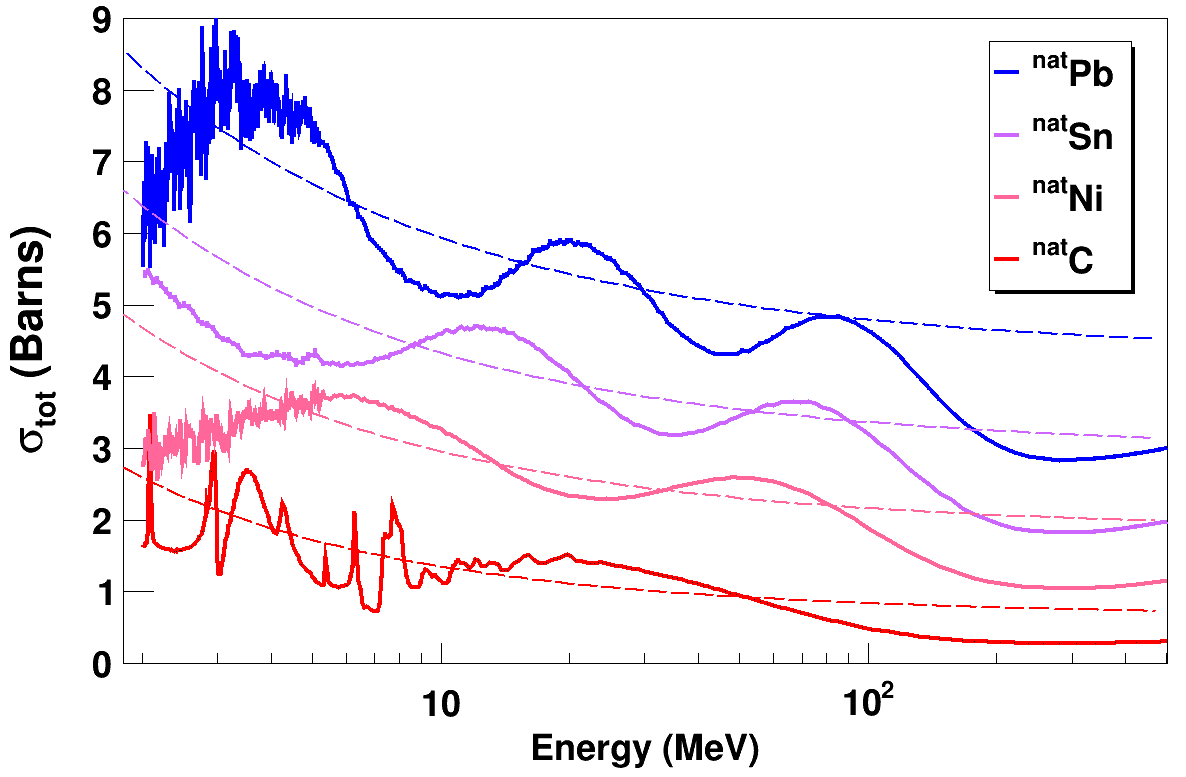
\includegraphics[width=0.9\textwidth]{figures/SASphereVsExperiment.png}
    \caption[Experimental neutron \tot\ data and strongly-absorbing-sphere predictions]
    {
        Experimental neutron \tot\ data on several natural samples (solid lines)
        from 2-500 \mega\electronvolt. The predictions of the crude strongly-absorbing-sphere
        model (Eq. \ref{SASAbsolute}) are shown as dashed lines. Resonance structures are
        clearly visible in the \cNat neutron \tot\ below 20 \mega\electronvolt.
    }
    \label{SASphereVsExperiment}
\end{figure}
These hallmark oscillations in the neutron \tot\ can be explained as the result
of a phase shift between 
neutron waves passing around the nucleus (unshifted) and waves passing
through the the nucleus, where they experience refraction
(illustrated in Fig. \ref{RamsauerPhaseShiftFigure}). This explanation was termed the ``nuclear 
Ramsauer effect'' by Peterson \cite{Peterson1962}, based on the analagous effect seen in 
electron scattering on noble gases.

Following Angeli \cite{Angeli1970}, these considerations can be incorporated by
imbuing the strongly-absorbing sphere relations (equation \ref{SASAbsolute}) with an additional sinusoidal term:
\begin{equation} \label{OscillatoryModel}
    \tot = 2\pi (R+\lambdabar)^{2}[1 - \rho \cos(\delta)]
\end{equation}
where $\rho = e^{-\operatorname{Im}(\Delta)}$, and $\delta =
\operatorname{Re}(\Delta)$, with $\Delta$ the phase difference between the wave traveling
around and traveling through the nucleus. Thus, the amplitude of the oscillation provides the 
elastic removal, or inelastic, phase shift and the period of oscillation
provides the elastic phase shift.
As can be seen from Eq. \ref{OscillatoryModel}, the large magnitude of the oscillations means that 
inelastic scattering (from $\operatorname{Im}(\Delta)$) accounts for only a small fraction of the 
total cross section, in turn implying a much larger mean free path for neutrons through the nucleus 
than would be expected in the absence of Pauli blocking \cite{Mohr1955}.

If the nucleus presents a spherical potential of radius $R$ and depth $U$, the total phase shift $\delta$ is:
\begin{equation} \label{phaseShift}
    \delta =
    \frac{\overline{C}\left(\left[{\frac{E+U}{E}}\right]^{\frac{1}{2}}-1\right)}{\lambdabar}
\end{equation}
where $\overline{C} = \frac{4}{3}R$ is the average chord length through the
sphere \cite{Angeli1970}. Rearranging Eq. \ref{phaseShift} in terms of A and E and
discarding leading constants yields:
\begin{equation}
    \delta \propto A^{\frac{1}{3}}\times\left(\sqrt{E+U}-\sqrt{E}\right)
\end{equation}
This form reveals an important relation: as A is increased, to maintain constant 
phase $\delta$, E must also increase \cite{Satchler1980, Peterson1962}. 
This is contrary to a typical resonance condition where an integer number of wavelengths
are fit inside a potential; in that case, to maintain constant phase as size is increased,
E must be decreased. Thus these \tot\ oscillations have been referred to as
``anti-resonances'' or ``echoes'' \cite{Satchler1980, McVoy1967}. It should be
noted that this simple Ramsauer picture is illustrative only, as it fails to
account for interference between the partial waves of the incident nucleon and
cannot be extrapolated to high energies without conspicuous deficiencies
\cite{Ahmad1973}.

A new type of nuclear model is thus at hand:
by replacing the intractable many-body problem
of the target nucleus by a complex, refractive potential, both elastic scattering (from the real 
part of the potential) and inelastic scattering (from the imaginary part) can be neatly 
explained. The existing mathematical machinery for calculating scattering of light from
refractive materials can then be repurposed for nuclear scattering, giving birth to
the ``optical model'' of the nucleus \cite{Feshbach1958, McVoy1967}.
Instead of a single central \gls{optical potential}, a series
of potential terms may be used,
centered on the nuclear surface and nuclear volume,
corresponding to differing physics thought to be relevant for these areas (much
as in the Droplet Model). Many comprehensive overviews of optical models are
available \cite{Dickhoff2018, Hodgson1971} that explore various potential forms
and connect optical models to other approaches.

\begin{figure}[tb]
    \centering
    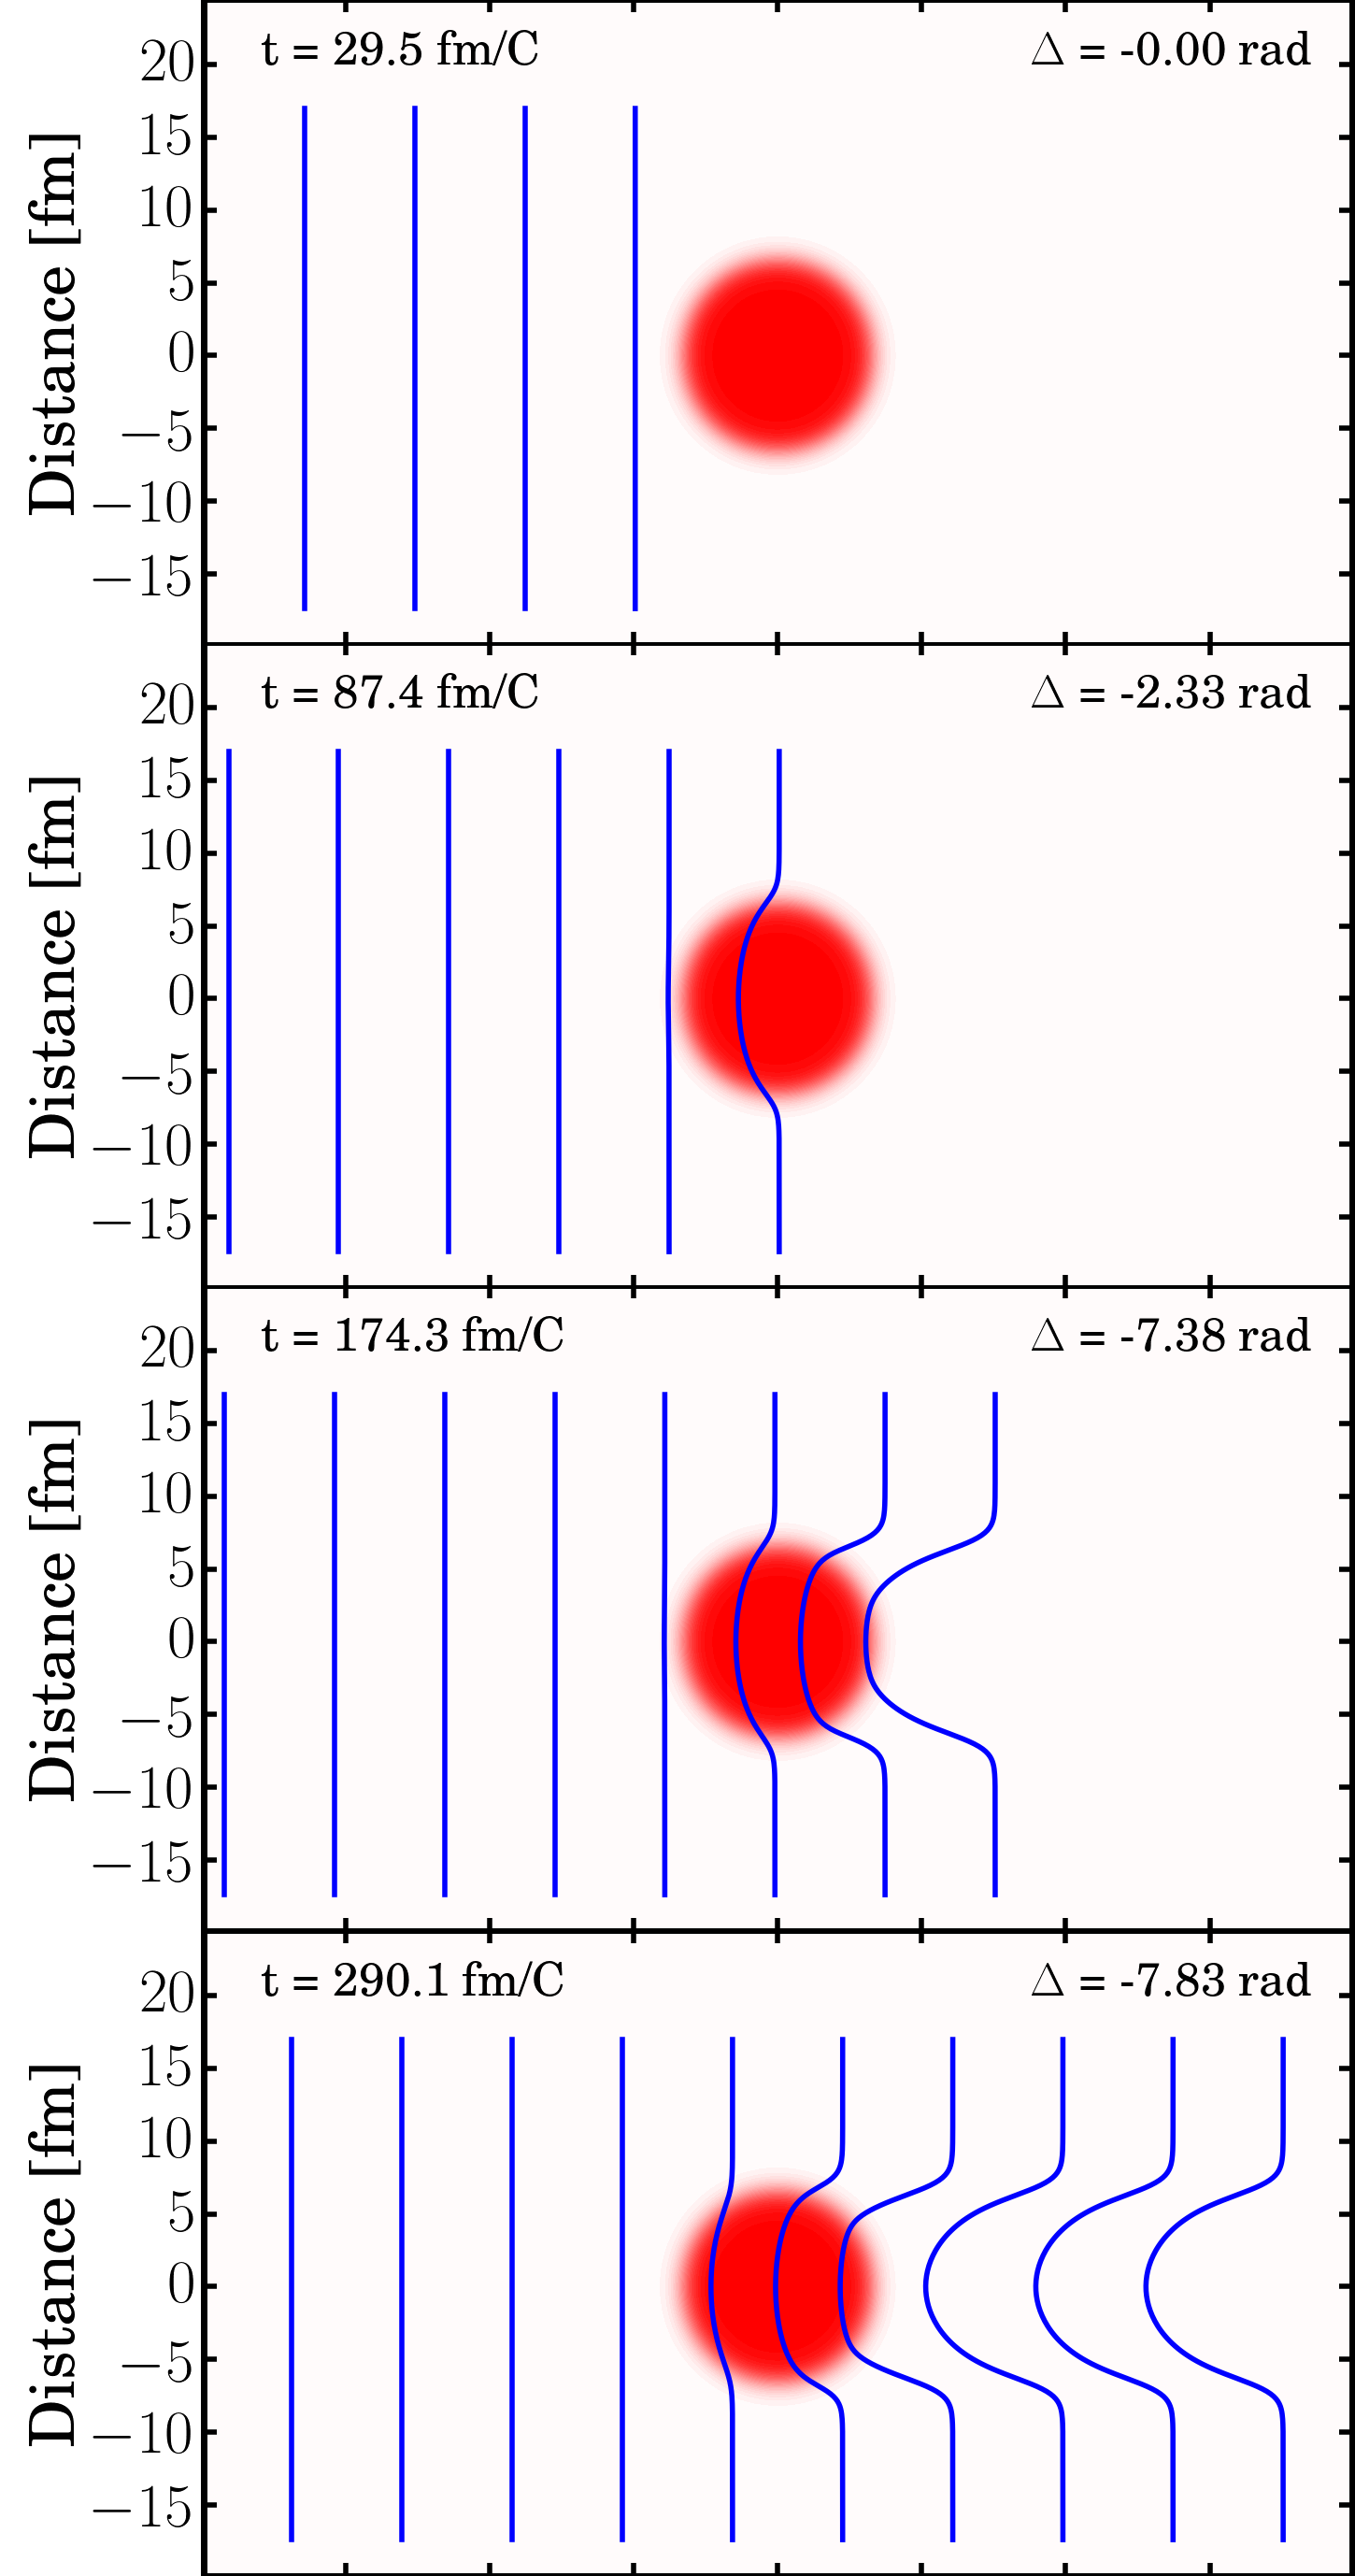
\includegraphics[height=0.7\textheight]{figures/phaseShiftStillsFigure.png}
    \caption[A illustration of the nuclear Ramsauer effect]
    {
        A neutron wave train (series of
        blue lines) impinges from the left on a real Woods-Saxon
        potential centered at the origin (diffuse red circle). The potential
        refracts the neutron wave,
        retarding the phase of the wavefront as it passes through the
        potential. After escaping the potential, a phase difference $\Delta$ between
        the wave component passing \textit{around} and \textit{through the center}
        of the potential persists, resulting in scattering.
        For the leading wavefront in the wave train, $\Delta$ is indicated in
        the top right-hand corner of each panel. A differential version of
        Eq. \ref{phaseShift} is used to
        calculate the phase shift for each step. In this figure, the neutron
        energy $E_{n}$ = 14 \mega\electronvolt\ and nuclear mass $A$ = 25. For the Woods-Saxon potential,
        we used a potential depth $U$ = 42.8 \mega\electronvolt\ (following Angeli and Csikai's analysis
        of \tot\ data at 14 \mega\electronvolt\ \cite{Angeli1970}), with nuclear radius $R = 
        r_{0}A^{\frac{1}{3}}$, $r_{0}$ = 1.4 fm, and a diffuseness parameter
        $a$ of 0.5 fm.
    }
    \label{RamsauerPhaseShiftFigure}
\end{figure}

Global OMs have been developed to simultaneously reproduce single nucleon, heavy ion,
and other hadron scattering data on targets across the chart of nuclides up to several
hundred \mega\electronvolt\ \cite{CH89, KoningDelaroche}. Because the proton-proton,
proton-neutron, and neutron-neutron scattering cross sections
are not identical, OM potentials are expected to differ for protons and
neutrons. Isoscalar terms, which respect isospin symmetry and thus treat protons and neutrons 
identically, account for most of the observed scattering, but do not include
the asymmetry-\textit{dependent} interactions known to exist between
nucleons, such as charged meson exchange.
Thus isovector and isotensor terms,
which depend on the difference between the proton and neutron density
distributions in the nucleus, are needed. As experimental facilities like
the Facility for Radioactive Isotope Beams (FRIB) come online and produce
extremely asymmetric nuclei, knowing the asymmetry-dependence of optical
potentials will become increasingly important for predicting nucleon scattering on
exotic nuclei. Isovector considerations are not unique to full-blown optical
models and can be introduced to a simpler Ramsauer-like models as well. For example, building
on the addition of spin-spin terms a Ramsauer model by Gould et al. \cite{Gould1986},
Anderson and Grimes added an explicit isovector term to analyzing isotone and isotope shifts in 
neutron total cross sections \cite{Anderson1990}.
They concluded that ``although [their] model may give
semiquantitative agreement with some aspects of the data, optical-model
calculations should be used for quantitative comparison''.

Despite their excellent reproduction of experimental data,
OMs involve the interaction of
many sometimes-opaque parameters with many incident
partial waves, blurring the intuitive picture of the underlying physics.
OMs are unabashedly phenomenogical so a wide variety of
experimental data types and energies are required to constrain the potential,
so when data are absent, model predictions are poor. Without a clearer connection to formal
many-body methods, the empiricism of optical models does clarify the connection between nuclear
reactions and nuclear structure. A major step forward was taken by Mahaux and Sartor
\cite{Mahaux1991}, who linked the nucleon self-energy to the \gls{optical potential} by means of a
dispersion relation, allowing for a more-direct comparison between scattering data and mean-field nuclear
structure calculations. We employ a descendant of their
dispersive optical model, generalized to include a
fully non-local potential, to treat nuclear structure and reactions on the same
footing.

A long-standing difficulty in optical-model analyses is in constraining the isovector dependence
of the real and imaginary parts of the potential \cite{Holt16, Anderson1990}. Improving constraints on the
isovector terms in particular requires data
on asymmetric nuclei, preferably on highly-asymmetric nuclei or isotopic chains,
where the imbalance of protons and neutrons makes any isovector effects most visible. The isovector
strength of the nuclear potential is directly connected to a host of open problems in nuclear physics,
including fixing the density-dependence of the symmetry energy, $L$, locating the
neutron dripline, and understanding how high-momentum content is distributed between neutrons and
protons. Making progress in this area requires improved experimental data sets
and is the main concern of the following section.

\section{Relevant Experimental Nuclear Data}

\subsection{Nucleon scattering data}
Elastic nucleon scattering cross sections, especially with protons, comprise the most extensively-measured
sector of experimental scattering databases. The EXFOR experimental reaction database
\cite{EXFORDatabase} contains thousands of proton and neutron
differential elastic scattering and analyzing
power data sets between 1-300 \mega\electronvolt, the domain relevant for this work. Optical model fits
to these data, both regional and global \cite{CH89, KoningDelaroche}, have helped
constrain nuclear radii, the strength of the spin-orbit coupling,
and revealed the importance of an imaginary spin-orbit term.

Inelastic nucleon scattering data are more difficult to collect experimentally and much sparser in
the literature record. By helping fix the strength and energy-dependence of the absorptive component
of the nuclear potential, inelastic data serve a complementary role to elastic
data.
%The was pointed out by Finlay et al. in 1993:
%\begin{displayquote}
%    ``Above about 200 \mega\electronvolt, an impulse approximation might be expected to
%    give a good description of the data, while at lower energy Pauli blocking and
%    medium effects must be included. Phenomenologically, the imaginary term in
%    the optical potential increases rapidly, while the real term is thought to
%    pass through zero \cite{Finlay1993}.''
%\end{displayquote}
\noindent
Isotopically-resolved data is particularly valuable for constraining nuclear
models, as it avoids averaging over multiple isotopes naturally present in many elemental samples.
Unfortunately, many pure isotopes are extremely expensive ($>$\$10,000 per gram) to
separate, putting them out of reach for all but the most well-funded experiments.
Indeed, as late as 1988, only a handful of neutron \tot\ measurement campaigns
on multiple samples had been conducted, most of them elemental, not isotopic
\cite{BarnBook1988}.

Figs. \ref{TCSChart} and \ref{RCSChart} illustrate the status of isotopically-resolved inelastic
nucleon scattering data in the EXFOR nuclear reaction database as of 2019.
Except for light isotopes and a few security-related actinides, coverage is
sparse and has changed little since the early 2000s. The single notable
exception is the triplet of $^{182,184.186}$W data sets from 5-560 \mega\electronvolt\ of \cite{Dietrich2003}, 
mentioned in the previous section. Isotopic \textit{proton} \rxn\ measurements over
a broad energy range are particularly lacking due to the paucity of suitable
accelerators and the subtlety of such a measurement. 
Both high-energy ($>$100 \mega\electronvolt) neutron \tot\ and proton \rxn\ data are useful for
understanding the asymmetry-dependence of the imaginary strength of the nuclear potential.
In this work, we focus on isotopically-resolved neutron scattering, which
is easier to measure and, when combined with proton \textit{elastic} cross sections,
also provides information on the asymmetry-dependence of the real part of the nuclear potential.

\begin{sidewaysfigure}
    \centering
    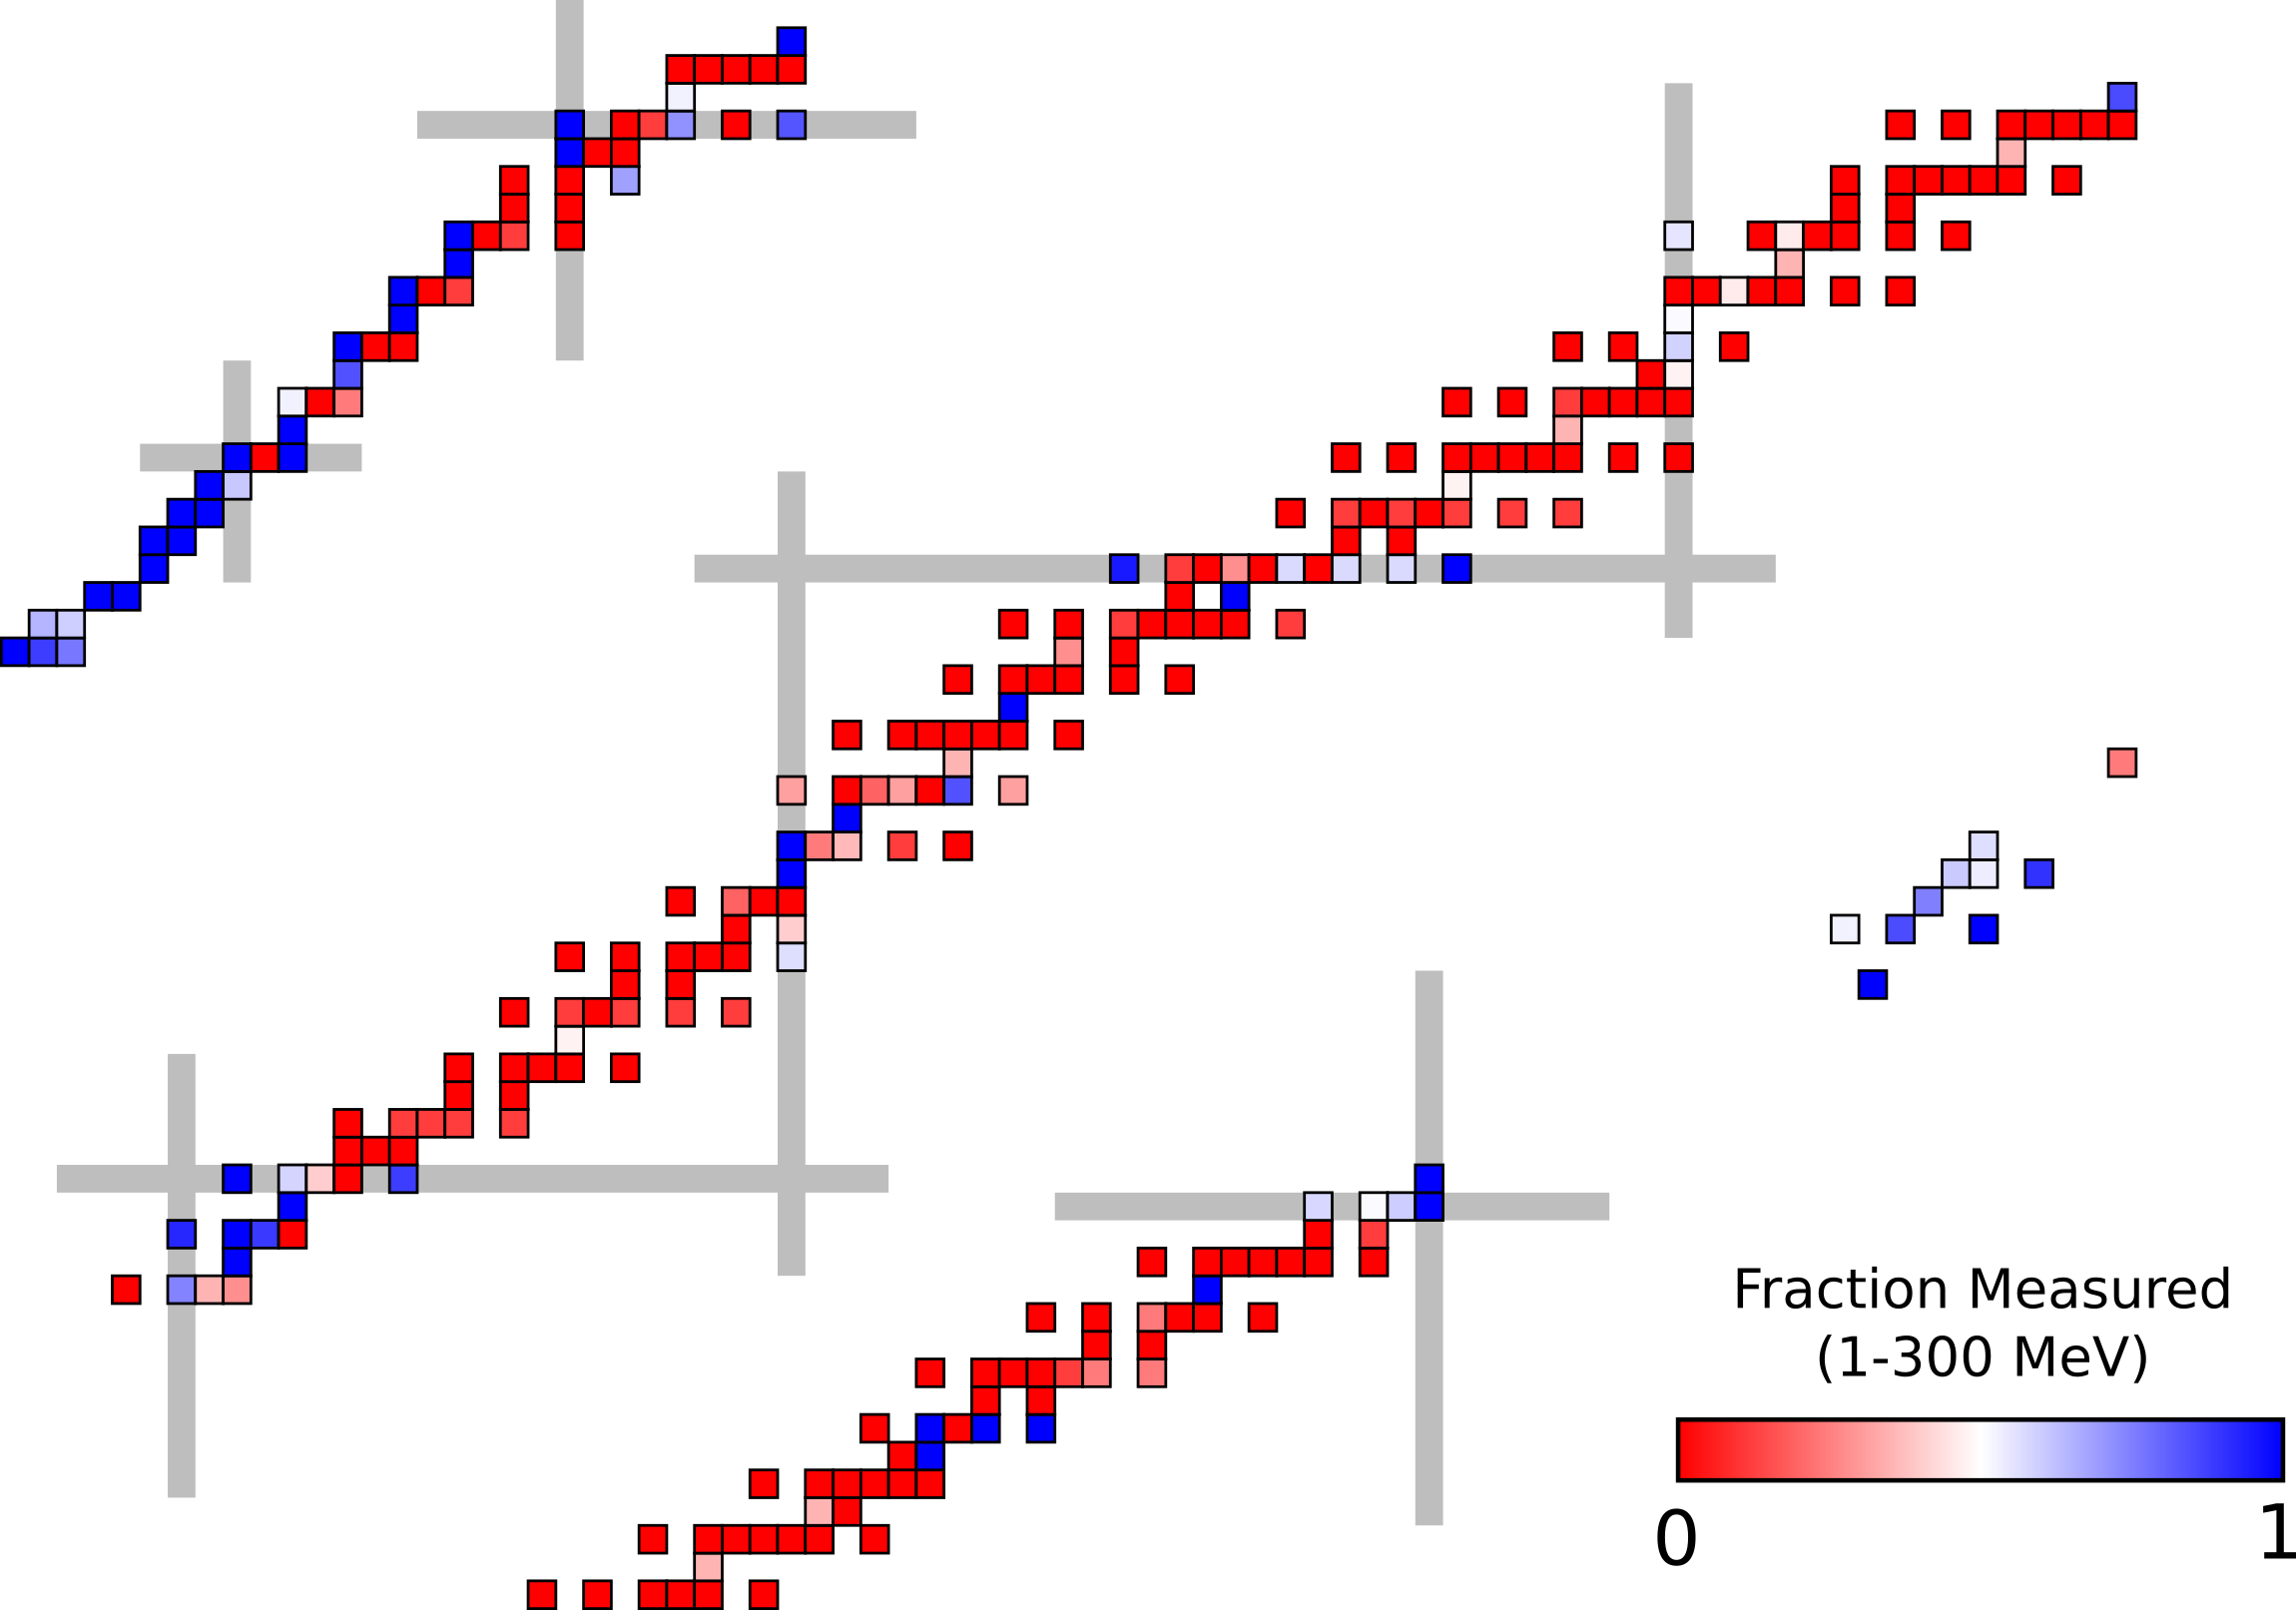
\includegraphics[width=0.9\textwidth]{figures/TCSChart.png}
    \caption[Landscape of existing neutron \tot\ data in 2019]
    {Isotopes are color-coded by the amount of neutron \tot\ data available in the EXFOR nuclear
        reaction database from 1-300 \mega\electronvolt, as accessed in 2018 and 2019. If data exists thoughout the
        1-300 \mega\electronvolt\ range, the isotope
        is colored blue. If no data exists, the isotope is colored red. For
        isotopes with partial coverage in this range, color varies by the degree
        of coverage. Except for the lightest
        isotopes (O and below), a few security-related actinides, there is almost no coverage
        throughout the nuclear chart. Our newly-measured results on \oSixEight, \niEightFour,
        \rhThree, and \snTwelveFour\ are included, as are a previous experiment
        by our group on \caAughtEight \cite{Shane2010}.
    }
    \label{TCSChart}
\end{sidewaysfigure}

\begin{sidewaysfigure}
    \centering
    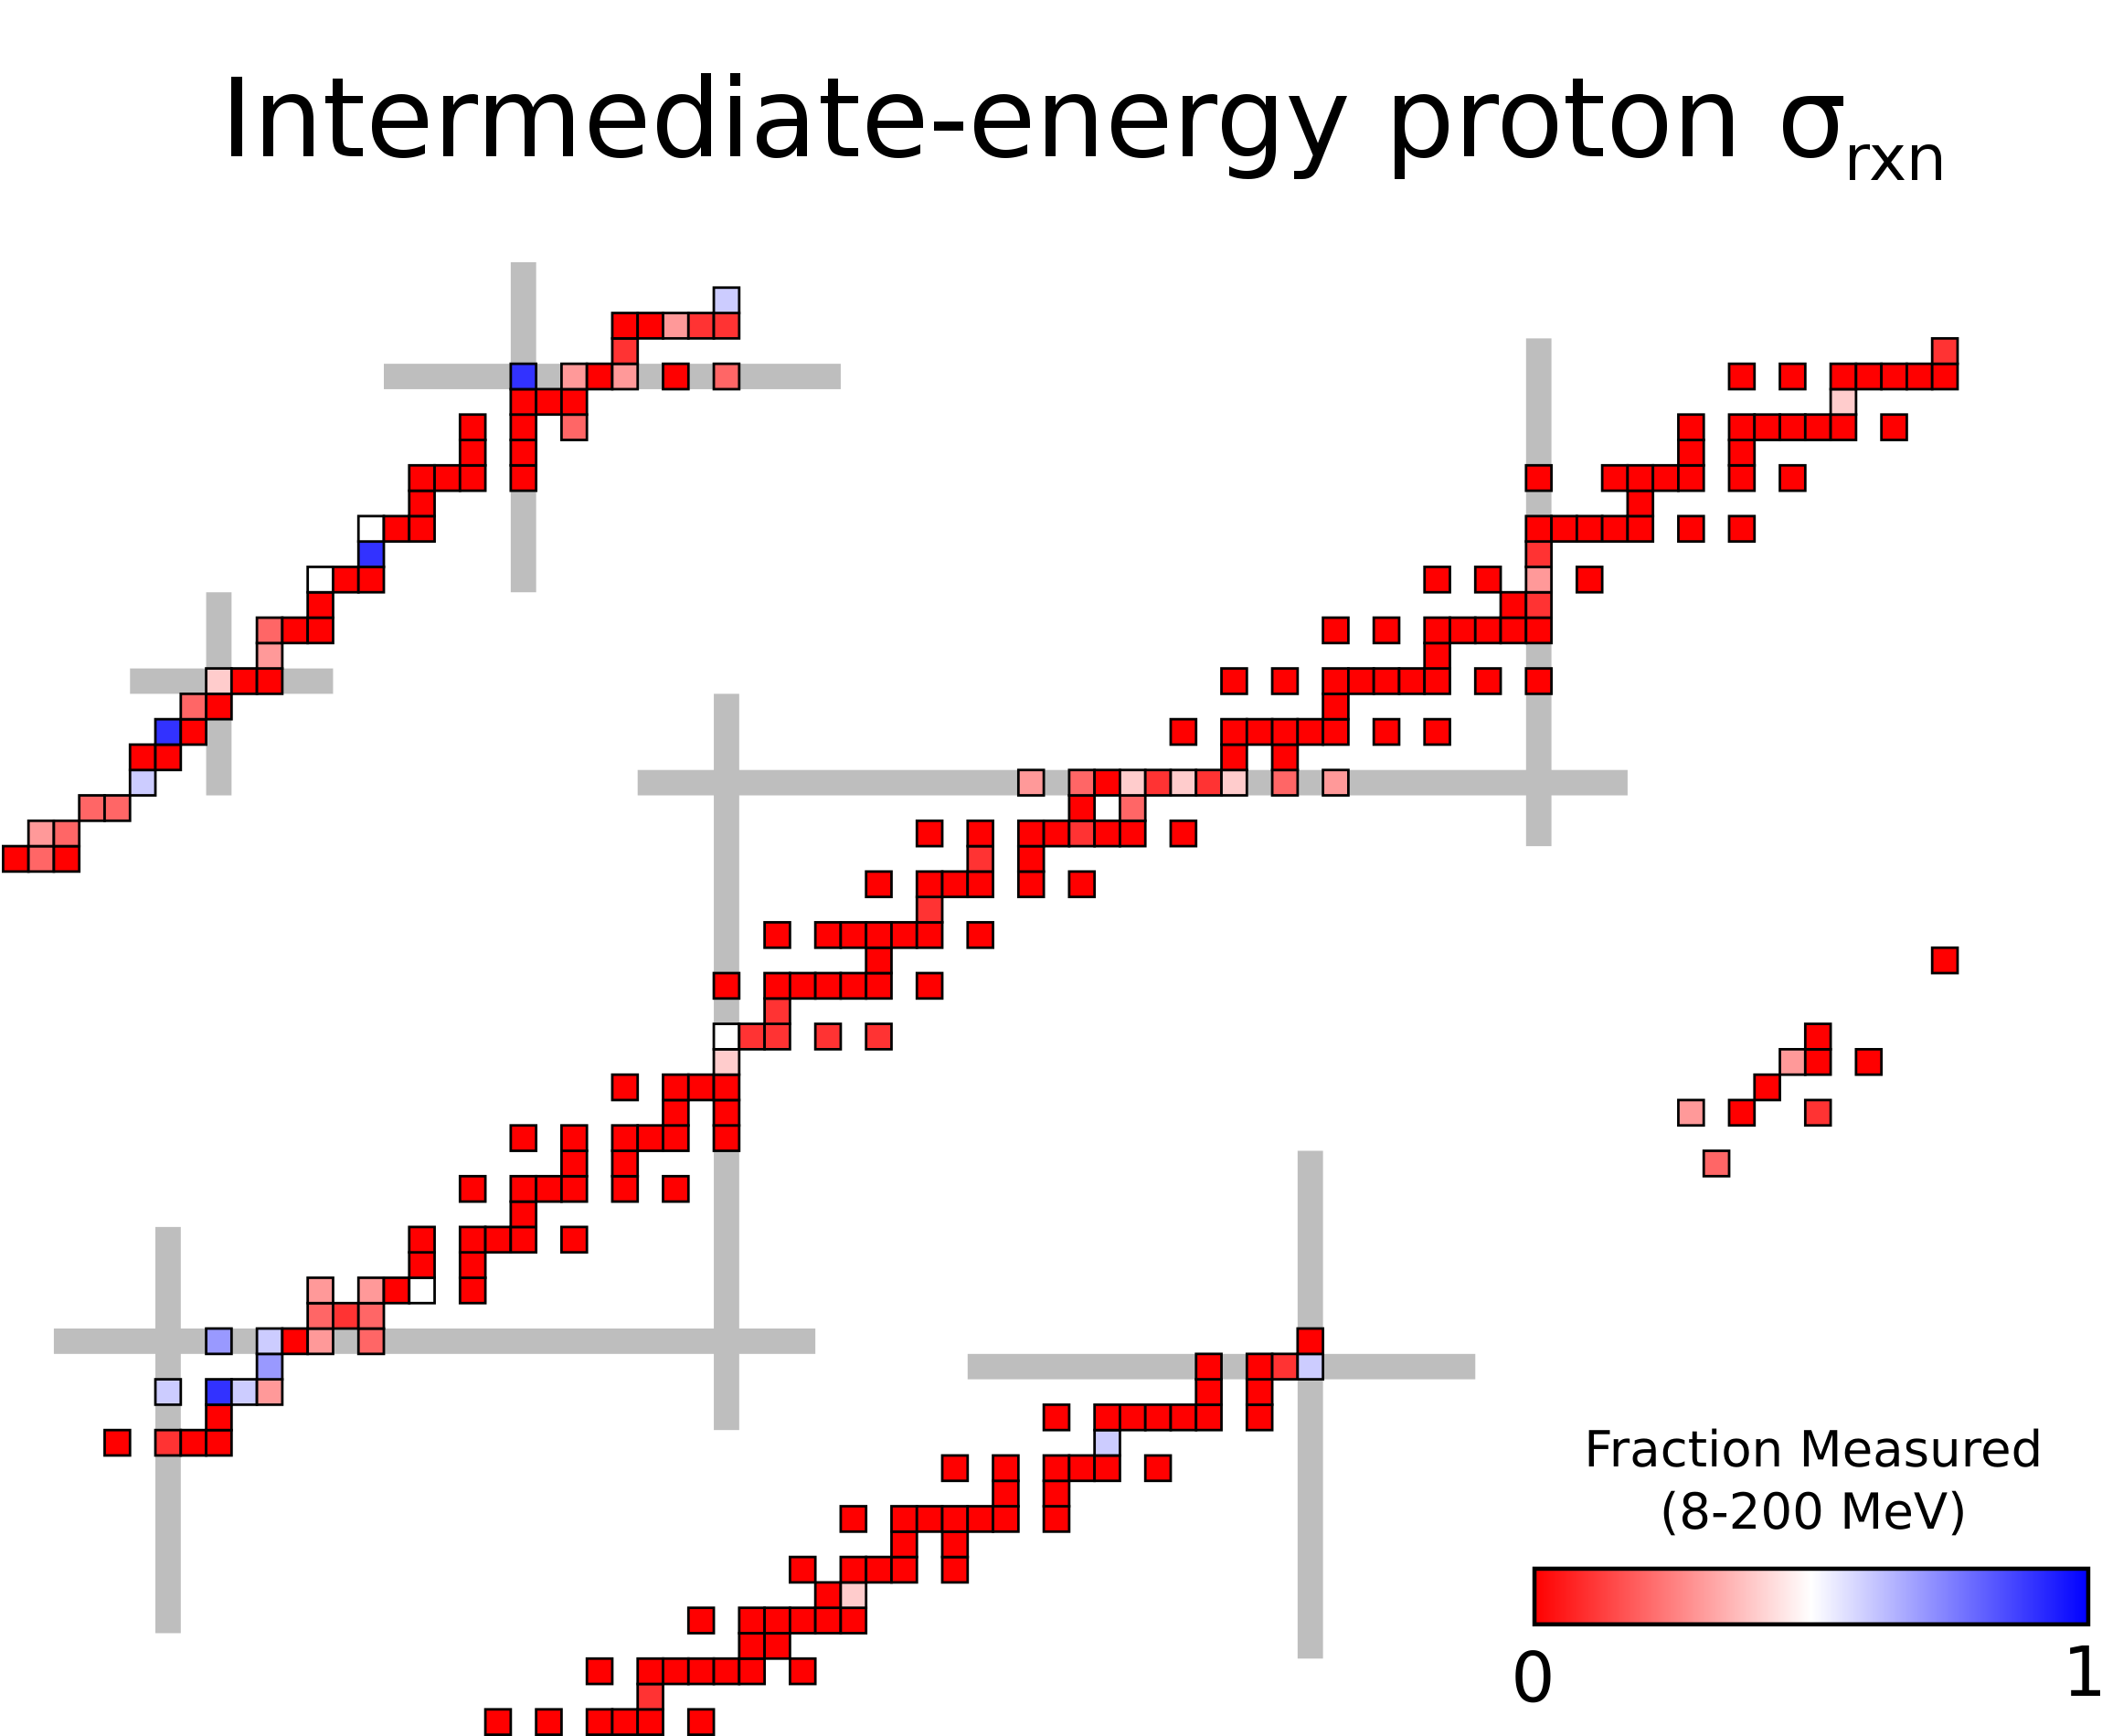
\includegraphics[width=0.9\textwidth]{figures/RCSChart.png}
    \caption[Landscape of existing proton \rxn\ data in 2019]
    {Isotopes are color-coded by the amount of neutron \tot\ data available in the EXFOR nuclear
        reaction database from 1-300 \mega\electronvolt, as accessed in 2018 and 2019. If data exists thoughout the 1-300 \mega\electronvolt\ range, the isotope
        is colored blue. If no data exists, the isotope is colored red. For
        isotopes with partial coverage in this range, color varies by the degree
        of coverage. Almost no nuclei have experimental coverage throughout this energy
        range, a testament to the difficulty of proton \rxn\ measurements.}
    \label{RCSChart}
\end{sidewaysfigure}

In the last few decades, a smattering of isotope-chain neutron total cross section
analyses have been carried out \cite{Mukhopadhyay2011, Anderson1990, Camarda1984}. The most sophisticated
was conducted by Dietrich et al.\cite{Dietrich2003},
using new data they measured on the $^{182,184,186}$W isotope chain (quite noticeable in Fig.
\ref{TCSChart}). In their study, an expanded Ramsauer-type model performed quite well at reproducing the relative 
difference between $^{186}$W and $^{182}$W, apart from a
phase mismatch - but only when the isovector components they introduced in the
Ramsauer model are \textit{suppressed} (see Fig. \ref{Dietrich2003_Ramsauer}). Despite the
dubiousness of ignoring isospin, the resulting Ramsauer model
agrees better with the experimental data than does the Ohio global optical 
potential \cite{Rapaport1979}, shown in Fig. \ref{Dietrich2003_Ohio}.

\begin{figure}[tb]
    \centering
    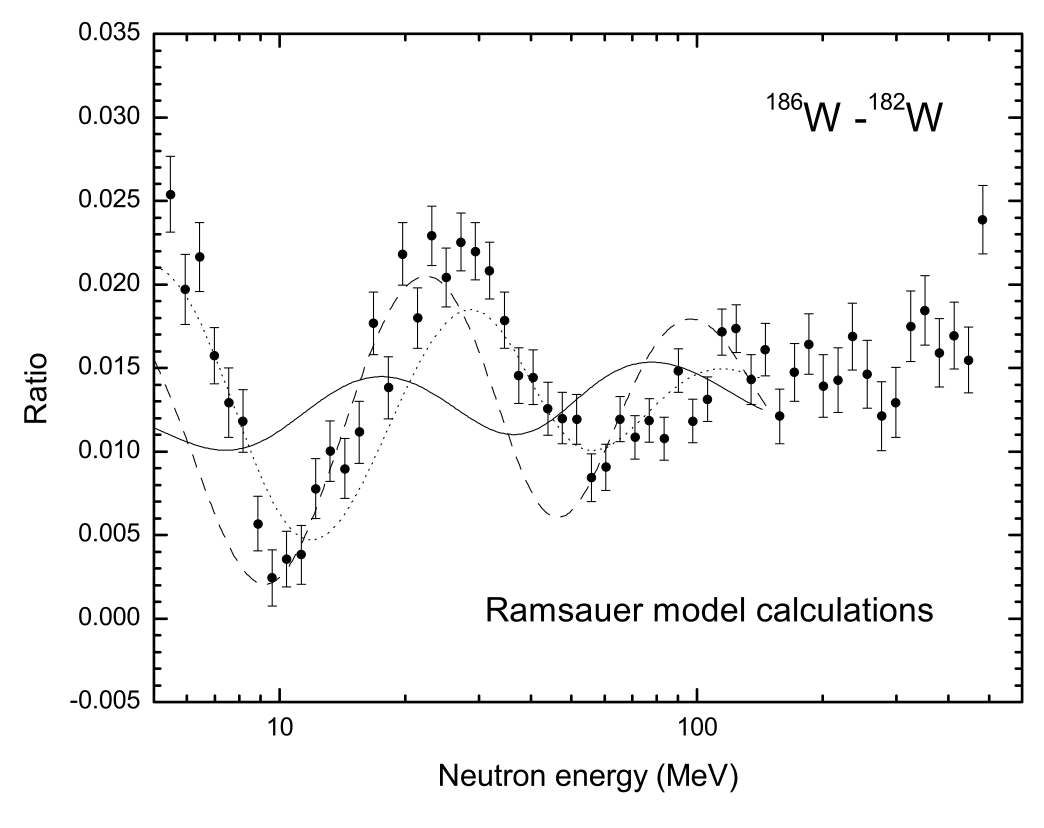
\includegraphics[width=0.8\textwidth]{figures/Dietrich2003_RamsauerPotential.png}
    \caption[$^{186}$W-$^{182}$W neutron \tot\ relative difference and
    Ramsauer model predictions]
    {
        $^{186}$W-$^{182}$W neutron \tot\ relative difference and
        Ramsauer model predictions. Figure from \cite{Dietrich2003}.
        If the standard isovector strength from
        optical-model treatments is used to dictate the Ramsauer isovector
        dependence (solid line), the model performs more poorly against the experimental
        data. When the isovector strength is suppressed, the correspondence to data improves (dashed
        line).
    }
    \label{Dietrich2003_Ramsauer}
\end{figure}

\begin{figure}[tb]
    \centering
    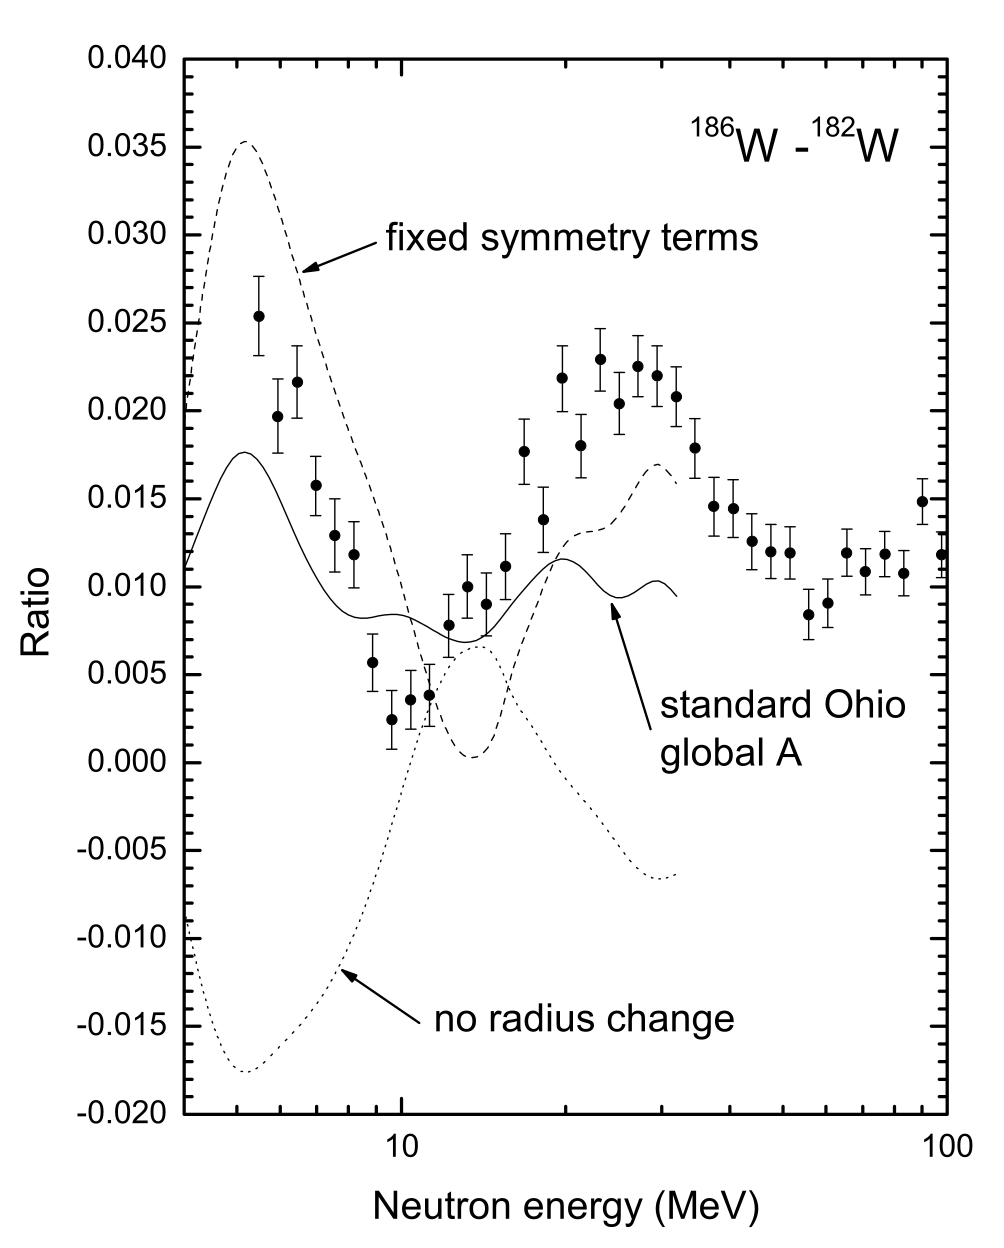
\includegraphics[width=0.6\textwidth]{figures/Dietrich2003_OhioPotential.png}
    \caption[$^{186}$W-$^{182}$W neutron \tot\ relative difference and
    Ohio global optical model predictions]
    {
        $^{186}$W-$^{182}$W neutron \tot\ relative difference and
        Ohio global optical potential predictions. Figure from \cite{Dietrich2003}.
    }
    \label{Dietrich2003_Ohio}
\end{figure}

The authors also performed phenomenological coupled-channel calculations
based on a dispersive optical model formalism
\cite{Mahaux1991} that showed similar behavior: it gave good agreement with the
experimental \tot\ relative differences, but only when isovector terms in the calculations
were explicitly \textit{neglected}. As the
authors point out, it is quite puzzling that ``good agreement with the
experimental data can be obtained at the expense of an incorrect physical
picture''.
Of the models they tested, only a deformed, semimicroscopic
optical model potential (SMOMP),
obtained by folding an energy- and density-dependent optical model potential from nuclear matter 
calculations over the deformed nuclear densities, was capable of satisfactorily describing the
\tot\ isotope shift in W. From this case study on W isotopes, several followup questions
are apparent: is a microscopic knowledge of the proton and neutron matter
densities important for reproducing the neutron \tot\ across an isotope
chain? More fundamentally, what terms in an optical potential are the neutron
\tot\ cross sections sensitive to, and are neutron \tot\ data connected to
structural (i.e., bound-state) information in a consistent, transparent way?

Answers to these questions hinge on the availability well-measured 
isotopic neutron \tot\ data sets across a broad energy range. Indeed, the
\caAughtEight\ neutron \tot\ data collected by our group at LANSCE in 2009, in
part inspired by the W measurements of \cite{Dietrich2003},
provided grist for a non-local Dispersive Optical Model (DOM) analysis in 2015
\cite{MahzoonPhDThesis}. This non-local analysis revealed connections
between the asymmetry-dependence of single-particle occupation numbers
and high-energy scattering data.
Providing experimental data on key nuclei, in particular for use with the \gls{DOM},
is a primary motivation for the isotopically-resolved neutron \tot\ and \el\
results presented in this work. These new data are analyzed in Chapter \ref{DOMResults} 
with an improved non-local DOM capable of fits to data on even-even nuclei. Details on our DOM
implementation are presented in chapter \ref{DOMFormalism}. 

\subsection{Nuclear Masses, Matter Radii, and Charge Radii}
The mass and spatial extent of a nucleus are two of its most fundamental
properties. Of all experimental data, nuclear masses are known to the highest
precision, up to ten significant digits \cite{AME2016}. Connecting masses and
radii is a central design of the Liquid Drop Model and many other theoretical
treatments over the last century (e.g., Hartree-Fock-BCS treatment of 700 nuclei to calculate 
proton and neutron RMS radii \cite{Angeli1980}). Extracting nuclear radii from optical
models have been an active area of research for over fifty years \cite{Jackson1974}.

Experimentally, a variety of techniques are available to probe the nuclear
charge density distribution. On stable nuclei, x-ray energies from muonic atoms
\cite{Fricke2004} are sensitive to deviations of the nuclear charge
distribution from sphericity, and elastic electron
scattering data can be used, after Fourier transform, provide the full nuclear
charge density profile at spatial resolutions between $\frac{2\pi}{q_{min}}$ and
$\frac{2\pi}{q_{max}}$, where $q$ is the momentum transfer associated with the
elastic scattering \cite{DeVries1987}.
On unstable nuclei, collinear laser spectroscopy \cite{Miller2019},
uses small shifts in electronic levels to extract
the difference in RMS radii ($\delta_{RMS}$) of the charge
distributions along an isotope chain, the so-called ``isotope shift''.
The isotope shift is shown for the even-A Sn isotopes in Fig.
\ref{SnIsotopeShift} \cite{Anselment1986}.
\begin{figure}[tb]
    \centering
    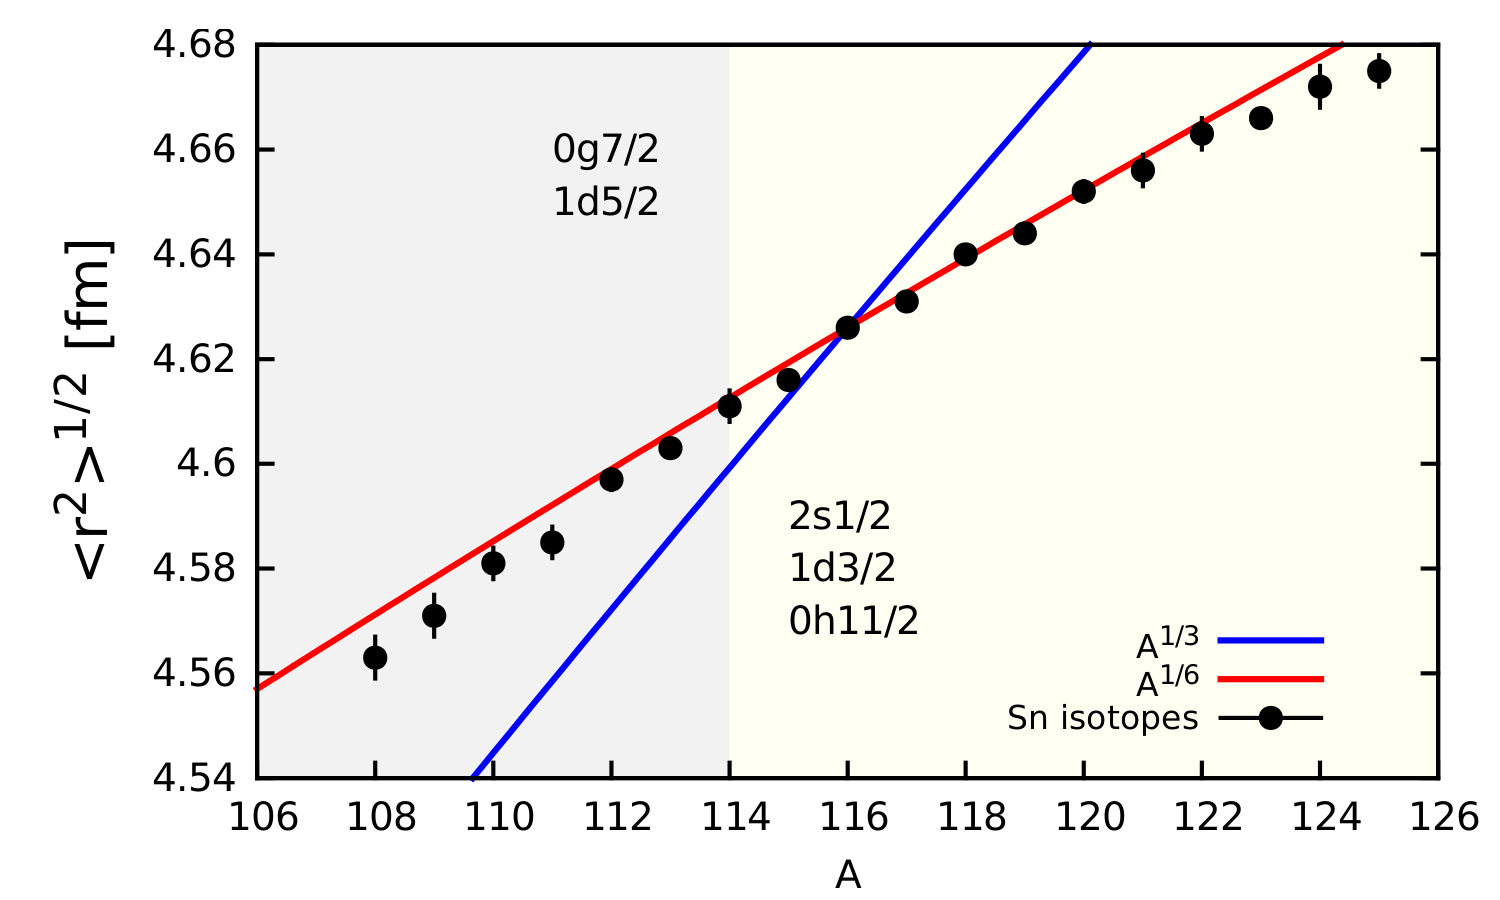
\includegraphics[width=0.9\textwidth]{figures/SnIsotopeRMSRadii.png}
    \caption[Root-mean-squared charge radii of Sn isotopes]
    {
        Root-mean-squared (RMS) charge radii in Sn isotopes.
        The A=106-114 region and A=114-116 region are shaded and labeled
    indicating the expected single-particle occupation of the valence neutrons.
    An isoscalar treatment that only accounts for size scaling predicts an
    A$^{\frac{1}{3}}$ slope as neutrons are added, but the data show a nearly-linear
A$^{\frac{1}{6}}$ slope instead. The slope of the isotope shift is connected to the symmetry energy
and its density dependence. Data from Anselment et al. \cite{Anselment1986}}.
    \label{SnIsotopeShift}
\end{figure}
It has long been clear that the 
isotope shift is critically connected to the neutron and proton matter distributions.
The difference in RMS radii between the protons and neutron point distributions
(i.e., not including the finite size of the protons and neutrons) is commonly referred to as the 
``neutron skin''  \cite{Otten1989} and was first identified as an important
nuclear quantity by Wilkinson over fifty years ago \cite{Wilkinson1967}.
In a Droplet Model picture, the slope of the isotope shift is linked to the symmetry energy $J$, 
density dependence of the symmetry energy
$L$, and surface stiffness coefficient $Q$\footnotemark, the same bulk quantities that determine
neutron-skin thickness \cite{MyersAndSwiatecki, Berdichevsky1988}.
\footnotetext{
    In \cite{MyersAndSwiatecki}, the $J$-, $L$-, and $Q$-dependent contributions to the
    binding energy are:
    \begin{equation*}
        \begin{split}
            E(N,Z;shape) & =
            [J\bar{\delta}^{2}-\frac{1}{2}K\bar{\epsilon}^{2}
            +\frac{1}{2}M\bar{\delta}^{4}]A\\
            & + \frac{9}{4}(J^{2}/Q)\bar{\delta}^{2}A^{\frac{2}{3}}B_{s}
            + CC(J,Q)
        \end{split}
    \end{equation*}

    \noindent
    where $\bar{\delta}$ and $\bar{\epsilon}$ of Eq.
    \ref{DropletIndependentQuantities} are fully parameterized as: 
    \begin{equation*}
        \begin{split}
            \bar{\delta} & = I+\frac{3}{16}(c_{1}/Q)ZA^{-\frac{2}{3}}B_{v}]
            /[1+\frac{9}{4}(J/Q)A^{-\frac{1}{3}}B_{s}]\\
            \bar{\epsilon} & = [-2a_{2}A^{-{\frac{1}{3}}}B_{s}+L\bar{\delta}^{2}
            +c_{1}Z^{2}A^{-\frac{4}{3}}B_{c}]/K
        \end{split}
    \end{equation*}
    
    \noindent
    In these equations, $K$ is the compressibility coefficient, $M$
    accounts for anharmonicity of the binding-energy dependence on $\bar{\delta}$,
    and $B_{s}$ accounts for shape dependence of the surface energy. $CC(J,Q)$ are
    corrections to the Coulomb term associated with deformation. The quantity
    $\frac{9}{4}(J^{2}/Q)\bar{\delta}^{2}$ is the correction to the binding
    energy from excess neutrons accumulating on the nuclear surface in neutron-rich
    systems (i.e., neutron skin formation).
}
\noindent
Without addition experimental constraints, the $J$, $L$, and $Q$ parameters form an
underdetermined system from which unique values cannot be recovered, even if the
consensus value of $J \approx$ 30 \mega\electronvolt\ is used to reduce the parameter space.
As was already pointed out 50 years ago by Myers \cite{Myers1969},
the single-particle configuration of a given nucleus may have a significant
effect on the formation and size of such a skin.

Charge radius measurements have
become sufficiently precise that models can no longer equate the proton matter
distribution and the charge distribution; the non-uniform charge distributions of the
proton and neutron must be accounted for as well. Constraining the neutron matter
distribution experimentally is extremely difficult, as neutrons do not interact
Coulombically with the electron and muonic probes used to determine the charge
distribution. An on-going, multi-year
experimental effort at Jefferson Laboratory aims to measure the \caEight\ and
\pbEight\ neutron and proton matter distributions directly using parity-violating electron
scattering, taking advantage of different weak charges of the proton and neutron
\cite{Horowitz2014}. The neutron skins of these and other neutron-rich nuclei
are of immense theoretical and astrophysical interest, as they are closely
correlated with the density-dependence of the symmetry energy, essential
for the neutron star equation-of-state, and with many other bulk properties of
nuclei, including the electric-dipole-polarizability (EDP) and the location of the
pygmy and giant dipole resonances (PDR and GDR)
\cite{Vinas2014, Brown2000, Fattoyev2012, Piekarewicz2012, Zhang2018}.
Constraining $L$ using these asymmetry-dependent 
properties is quite challenging: the properties of highly-asymmetric nuclei are
most closely correlated with $L$, but harder to measure experimentally, and the
properties of low-asymmetry nuclei are much more weakly correlated with $L$.
One of the chief goals of the Dispersive Optical
Model (detailed in Chapter \ref{DOMFormalism}) is to extract well-constrained values for the 
neutron skin thickness on a variety of nuclei (shown in Chapter
\ref{DOMResults}). By judiciously applying all available scattering and bound-state
data in the DOM approach, we hope to test the assertion
that the EDP, GDR location, neutron skin, and $L$ are as tightly correlated as
it appears from mean-field models.

\section{Motivation, Scope, and Dissertation Outline}
Improved isotopically-resolved neutron scattering data are an essential ingredient
for better nuclear reaction models and to test the asymmetry-dependence of the
nuclear potential. The results of our campaign to collect these valuable
\tot\ and \el\ data sets on cornerstone nuclei form the backbone of this dissertation.
In addition to these experimental results, a suite of Dispersive Optical Model analyses that 
incorporates these new data is presented. From the DOM potentials, a variety of asymmetry-dependent 
nuclear-structure quantities, including neutron skins and relative momentum
content, are extracted.

An overview of neutron \tot\ experimental considerations, the details of our 
\tot\ experiment, and analysis for our isotopically-resolved \tot\ measurements
on \oSixEight, \niEightFour, \rhThree, and \snTwelveFour\ are detailed in 
Chapters \ref{TCSExperiment} and \ref{TCSAnalysis}. Similarly, our elastic scattering measurements 
on \snTwelveFour\ are presented in Chapters \ref{ECSExperiment} and \ref{ECSAnalysis}. A brief 
summary of the Dispersive Optical Model formalism is
given in Chapter \ref{DOMFormalism} and the results from our DOM fits of \oSixEight, 
\caAughtEight, \niEightFour, \snTwelveFour, and \pbEight\ are presented in Chapter \ref{DOMResults}. 
A complete listing of the experimental data used in the DOM analyses, the
parameter values of the DOM potentials, and figures showing the 
results of the DOM fits are provided in Appendices \ref{DOMDataSets},
\ref{DOMParameters}, and \ref{DOMFits}. 


\chapter{Dispersive Optical Model Formalism} \label{DOMFormalism}
\section{The Single-Particle Propagator}
The central project of the Dispersive Optical Model (like any optical model) is
to understand how nucleons move about in a nuclear many-body system. Specifically,
we wish to know
how a nucleon with energy $E$ and quantum numbers $\alpha$
at time $t_{0}$ will be measured at a
later time $t$ with quantum numbers $\beta$ after its interaction with the
nuclear environment, which is modeled with an optical potential. Given the
Hamiltonian that incorporates this interaction, the Schr\"odinger equation
relates the Hamiltonian to the time evolution of this state:

\begin{equation}
    i\hbar\frac{\partial}{\partial t}\ket{\alpha, t_{0};t} = H\ket{\alpha,
    t_{0}; t}
\end{equation}

where $\ket{\alpha, t_{0},t}$ is the state at time $t$, given an initial state
$\ket{\alpha, t_{0}}$. Simple substitution shows that this initial state
propagates in time according to:

\begin{equation}
    \ket{\alpha, t_{0}, t} = e^{-\frac{i}{\hbar}H(t-t_{0})}\ket{\alpha, t_{0}}
\end{equation}

Concretely, given initial position quantum numbers $\bm{r}$, the wavefunction
of a state $\psi(\bm{r},t)$ is the sum of the contributions of 

\begin{figure}
    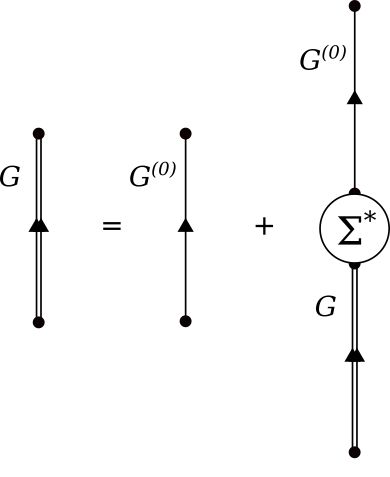
\includegraphics[scale=0.35]{figures/DysonEquation.png}
    \caption{The Dyson Equation in diagrammatic form}
    \label{DysonEquation}
\end{figure}

The Hartree-Fock potential, the default starting place for a mean-field potential,
has no energy dependence and thus cannot accommodate 

\section{Connection to Experimental Observables}
Subtracted dispersion relation.

\subsection{Elastic and inelastic nucleon scattering}
For nucleon-nucleus scattering, the scattering amplitude can be directly calculated using the
reducible self-energy:

\begin{equation}
    f_{m'_{s},m_{s}}(\theta,\phi) =
    -\frac{4m\pi^{2}}{\hbar^{2}}\braket{\boldmath{k}'m'_{s}|\Sigma(E)|\boldmath{k}m_{s}}
\end{equation}

\noindent
where $\boldmath{k}m_{s}$ are the wave vector and spin quantum number of the incident nucleon and
$\boldmath{k'}m'_{s}$ are for the exiting nucleon. The matrix structure of the right side can be
split into spin-independent and spin-dependent portions $\mathcal{F}$ and $\mathcal{G}$:

\begin{equation}
    \begin{split}
    f(\theta,\phi) & = \mathcal{F}(\theta)I + \sigma\cdot\boldmath{\hat{n}}\mathcal{G}(\theta)\\
    & = \frac{1}{2ik}\sum_{l=0}^{\infty}\left[(l+1)e^{2i\delta_{l+} - 1} +
    l\left(e^{2i\delta_{l-}}-1\right)\right]P_{l}(cos\theta) +
    \sigma\cdot\boldmath{\hat{n}}\left[\frac{sin\theta}{2k}\sum_{l=1}^{\infty}[e^{2i\delta_{l+}}-e^{2i\delta_{l-}}]P'_{l}(cos\theta)\right]
    \end{split}
\end{equation}
\noindent
where $P_{l}$

The phase shift (equivalently, the S-matrix elements) for each partial wave can be directly from the reducible self-energy:
\begin{equation}
    \begin{split}
        e^{2i\delta_{lj}} & \equiv \braket{k|\mathcal{S}_{lj}(E)|k}\\
        & = 1 - 2\pi i \left(\frac{mk}{\hbar^{2}}\right) \braket{k|\Sigma_{lj}(E)|j}
    \end{split}
\end{equation}
\noindent
where $k$ is the center-of-mass momentum of the nucleon, $m$ is the nucleon mass, and $E$ is the
center-of-mass energy. 
\subsection{Bound-state properties}

\section{Parameterization of the Potential}

To parameterize the DOM's optical potential, we rely on standard functional
forms common in nuclear theory calculations.

The real part of the potential is comprised of a Hartree-Fock component and
a spin-orbit component (plus a Coulomb term if the projectile is a proton).
The Hartree-Fock component $V_{HF}$ has two subcomponents:

\begin{equation}
    V_{HF}(r,r') = V_{vol}(r,r') + V_{WB}(r)
\end{equation}

The non-local Hartree-Fock volume term $V_{vol}(r,r')$, is defined as
a Woods-Saxon form coupled to a Gaussian non-locality:

\begin{equation}
    V_{vol}(r,r') =
    \dfrac{-V}{1+e^{(r-R)/a}}\cdot\dfrac{1}{\pi^{\frac{3}{2}}\beta^{3}}
    \exp{\frac{|r-r'|^{2}}{\beta^{2}}}
\end{equation}

where $V$, $R$, and $a$ are the depth, radius, and diffuseness of the HF potential,
and $beta$ is the extent of the non-locality. The local Hartree-Fock wine-bottle
term $V_{wb}(r)$, named for resemblence to the dimple at the bottom of a wine
bottle, is defined as a Gaussian centered at the nuclear origin:

\begin{equation}
    V_{wb}(r) = V\exp{\frac{r^{2}}{\sigma^{2}}}
\end{equation}

The real spin-orbit component $V_{so}$
is defined using a derivative-Woods-Saxon shape to
accommodate the expectation that the spin-orbit coupling is strongest near the
nuclear surface:

\begin{equation}
    V_{so}(r,r') =
    \frac{d}{dr} \frac{-V}{1+e^{\frac{(r-R)}{a}}}\cdot\frac{1}{\pi^{\frac{3}{2}}\beta^{3}} \exp{\frac{|r-r'|^{2}}{\beta^{2}}}
\end{equation}

The imaginary part of the potential is comprised of independent surface and volume terms
both above and below the Fermi surface, plus an imaginary spin-orbit term:

\begin{equation}
    V_{HF}(r,r') = V_{vol}(r,r') + V_{WB}(r)
\end{equation}

The occupation number of nucleons with quantum numbers $\alpha$ can be
calculated directly from the imaginary component of the single-particle
propagator:

\begin{eqnarray}
    n(\alpha)
    & = & \braket{\Psi^{N}_{0}|a^{\dagger}_{\alpha}a_{\alpha}|\Psi^{N}_{0}}\\
    & = & \sum_{n}|\braket{\Psi^{N-1}_{n}|a_{\alpha}|\Psi^{N}_{0}}|^{2}\\
    & = & \int_{-\infty}^{\epsilon_{F}^{-}} dE
\sum_{n}|\braket{\Psi^{N-1}_{n}|a_{\alpha}|\Psi^{N}_{0}}|^{2}
\delta(E-(E^{N}_{0}-E^{N-1}_{n}))\\
& = & \int_{-\infty}^{\epsilon_{F}^{-}} dE \frac{1}{\pi}\operatorname{Im}G(\alpha,\alpha;E)
\end{eqnarray}


For nuclei with open subshells (e.g., the $\upnu$ 0\dFive in $^{18}$O and
$\upnu$ 0\fFive in $^{58}$Ni), an additional
pairing parameter $\Delta$ was added to
account for these subshells' fractional occupatio $n_{\pm}$ of the open subshells. due to pairing
effects. This parameter splits partially-occupied subshells (e.g., the $\upnu$\dFive
for \oEight) into upper and lower sublevels with energies $E_{\pm}$:

\begin{equation}
    E_{\pm} = \mu \pm ((\epsilon_{F}-\mu)^{2} + \Delta^{2})^{frac{1}{2}}
\end{equation}

where $\mu$ is the energy of the open subshell before pairing is considered and
$\epsilon_{F}$ is the Fermi
energy. The magnitude of $\Delta$ corresponds to the energy difference between
adding/removing a nucleon to/from that subshell. The subshell's particle
capacity is split between the upper and lower sublevels, and only the :

\begin{equation}
    n_{\pm} = \frac{1}{2}\left( 1-\frac{\chi}{E_{\pm}}\right)
\end{equation}

where $\chi = |E_{\pm}-\mu| - (\epsilon_{F} - \mu)$. Only occupation in the
lower sublevel is counted toward the total particle number. For each open-shell
nucleus with nucleon numbers $N, Z$ , the pairing gap $\Delta$ was fixed according to:

\begin{equation}
    \Delta(N,Z) = \frac{1}{4}\left(B(N-2,Z)-3B(N-1,Z) + 3B(N,Z)-B(N+1,Z)\right)
\end{equation}

where $B(N,Z)$ is the nuclear binding energy.

The Dispersive Optical Model (DOM) is a phenomenological framework useful for 
extracting information about nuclear properties and structure from experimental
data.

The fundamental object of interest in the DOM is the \Gls{optical potential},
which is identified as the \Gls{nucleon self-energy}. This potential represents
the nuclear environment experienced
by a nucleon as it traverses the nucleus being represented. In general, the
potential is both non-local and complex, possessing both real (flux-conserving)
and imaginary (flux-removing) parts. The functions used to parameterize the optical potential
are selected to conform with general physical intuition about the nuclear
many-body problem and past experience with optical potentials throughout the
field. For example, the most important term, the Hartree-Fock (HF) potential
that binds the nucleus together, is defined by a classic Woods-Saxon form to
which non-locality has been added: [insert volume term formula]. The imaginary
potential is separated into a Woods-Saxon volume component and a
Woods-Saxon-derivative surface component. Each of these subcomponents has
a non-linear energy dependence reflecting our expectation that surface-like
behaviors should arise around 10-20 MeV and volume-like behavior should dominate
above 50 MeV, with a mixture of the two in the intermediate region.

Beyond these basic considerations, several additional features make the 
DOM a useful tool. First is the enforcement of a
dispersion relation (the Kramers-Kronig relations) between the real and imaginary
halves of the potential, ensuring that the potential is causal (i.e., the
time-ordering of the operator representation of the self-energy is maintained).

\section{Computational Improvements}
As with any high-dimensional optimization problem, the fitter must be vigilant
against the overfitting of data. In practice, this requires:

parsimony with the number of parameters used in the model

common-sense checking "under the hood" of the optimization to verify that
parameter values make sense given the assumptions that undergird the model

understanding of what the value function is (that is, the function being
minimized/maximized) and whether it needs to be changed

cross-correlation between parameters to understand the relationship between
parameters and the effect that each has on predictions made using the model

TCS affected by HF parameters, spin orbit, imaginary above
RCS affected by imaginary above, HF parameters
ECS affected by HF parameters, spin orbit, imaginary above
APower affected by HF parameters, spin orbit,  imaginary above
Charge Density affected by HF parameters, imaginary below
Levels affected by HF parameters, spin orbit,
Spectral functions affected by HF parameters, imaginary below
RMSRadii affected by HF parameters, imaginary below

Physical intuition about scattering data:
- the low-angle ECS/APower data are sensitive to the imaginary strength above
the Fermi surface. The high-angle ECS/APower data are sensitive to the imaginary
strength below the Fermi surface, with the highest angles of elastic scattering
probing the imaginary strength deepest in the core (see high-energy, high-angle
data in Pb)
- the NM correction to the imaginary volume strength is required in all cases to
have the very high/very low energy imaginary strength have the correct trend
(linearly increasing above 100 MeV above, decreasing to 0 below 100 MeV below).
Seen in spectral functions and total cross section data at high energies, where
the pion production channel enters the picture as it goes from virtual->real
- the general trend of the elastic scattering data (not wiggles, but averaged
over wiggles) depends on the imaginary strength at the given energy. If the
minima in the elastic cross sections are too sharp/deep, the imaginary strength
is too large at that energy
- the spin-orbit strength has dramatic effects on the total cross section at low
energies ($<$20 MeV)
- above the Fermi surface, the imaginary strength is dominated by surface from
0-50 MeV and by volume from 50 MeV up. Below the Fermi surface, the surface
imaginary strength is dependent on A; for low A, where the level density is very
low below the Fermi surface and there's almost no contribution from high LJ
levels, there is virtually no surface imaginary strength below (cf. with charge
density distribution tail, at the surface of the nucleus). As A increases, 
imaginary surface strength below increases gradually but never reaches the
imaginary surface strength above. A consequence of the asymmetry of the
operators that contribute: below 0 MeV, the removal operator LJs
must recouple to the ground state, so high LJ operators have virtually no
contribution; above 0 MeV, addition operators can have arbitrary LJs because
free scattering is possible, adding significantly to the collective strength and
thus is imaginary strength peaked at the surface in the 20-30 MeV range (giant
dipole resonance, for example, surface phonons).

\subsection{Fitting procedure}
The powell method, outlined in Numerical Recipes in C \cite{NumericalRecipes},
was used to minimize the RMS difference between experimental data points and the
values calculated by the DOM. A weighting scheme was assigned to the data points
according to their importance, guiding the fit to reproduce the most essential
data points. From fit to fit, the weighting scheme was adjusted as necessary to
escape local minima in the multidimensional fit.

The radial grid, energy grid, size of the lagrange basis, partial wave angular momentum cutoff, and
various integration cutoffs used in calculating the potential and
observable quantities were varied to ensure that output was not distorted by numerical errors. 

\subsection{Generalization to even-even nuclei}
- 

\afterpage{\clearpage}


\chapter{Neutron Scattering And Detection Techniques} \label{Techniques}
%\begin{figure}
%  \begin{center}
%  \includegraphics[width=0.8\textwidth]{Chart_of_Nuclides.pdf}
%  \caption{Figure caption}
%  \label{chart}
%  \end{center}
%\end{figure}

% \Gls{DOM} for glossary term
% \noindent for no indent

%\begin{comment}
% Woods-Saxon potential 
%\end{comment}
%
%\begin{equation}
%V(r) = \dfrac{-V_0}{1+e^{(r-R)/a}},
%\end{equation}

%\mathbf{J} = math bold-font symbol 'J'


\chapter{Neutron Total Cross Sections: Experiment} \label{TCSExperiment}
\section{Overview of neutron \tot\ experiments}

Neutron scattering is a direct, Coulomb-insensitive tool for probing the nuclear
environment. The simplest measurement of neutron interaction with a nucleus,
the neutron total cross section \tot, provides fundamental information about
nuclear size and the ratio of elastic-to-inelastic components of nucleon 
scattering. Additionally, \tot\ data are connected to a variety of nuclear
properties of great interest including the neutron skin of neutron-rich nuclei
\cite{Mahzoon2017} and thus the density dependence of the symmetry energy $L$,
essential for an accurate neutron star equation-of-state (EOS)
\cite{Fattoyev2012, Vinas2014, Brown2000}.

By scattering secondary radioactive beams off of hydrogen targets in \gls{inverse
kinematics}, proton-scattering experiments are possible even on highly unstable
nuclides. In contrast, because neutrons themselves must be generated as a
secondary radioactive beam, neutron-scattering experiments are restricted to
normal kinematics and \tot\ measurements are possible only for relatively stable
nuclides that can be formed into a target. At present, \tot\ measurements above
the resonance region on nuclides with short half-lives (shorter than the timescale of
days) are technically infeasible for this reason, though a handful have been carried out on
samples with half-lives in the tens to thousands of years \cite{Poenitz1983,
Phillips1980, Foster1971}.

\begin{table}[tb]
    \caption[Selected results from a literature study of
    isotopically-resolved \tot\ data using the EXFOR database \cite{EXFORDatabase}]
    {
        Selected results from a literature search for isotopically-resolved
        \tot\ data using the EXFOR database \cite{EXFORDatabase}.
        For the heaviest and lightest stable nuclides in each closed shell in Z, all
        datasets falling at least partially within
        1-500 \mega\electronvolt\ are shown. For elements
        whose natural abundance is $>$90\% of a single isotope (e.g.,
        96.9\% of $^{\text{nat}}$Ca is \caForty), \tot\ data on the natural
        sample was included as ``isotopic''.
    }
    \label{IsotopicCrossSectionTable}
    \centering
    \begin{tabular}{G N R@{\ --\ }l G}
        \toprule
        Isotope & \multicolumn{1}{c}{Nat. Abund. [\%]} & \multicolumn{2}{c}{Energies
    [\mega\electronvolt]} & Reference\\
        \midrule

        $^{3}$He & \multicolumn{1}{c}{2$\times$10$^{-4}$} & 1.5 & 40 & \cite{Haesner1983}\\
        $^{4}$He & \multicolumn{1}{c}{$>$99.9} & 0.7 & 30 & \cite{Goulding1973}\\
                 &                  & 2   & 40 & \cite{Haesner1983}\\
                 &                  & 77  & 151 & \cite{Measday1966}\\

        \oSix & 99.8                & 0.2 & 49 & \cite{Perey1972}\\
              &                     & 5   & 600 & \cite{Finlay1993}\\

        \oEight & 0.20 & 0.1 & 2.5 & \cite{Vaughn1965}\\
                & & 2.5 & 19 & \cite{Salisbury1965}\\

        \caForty & 96.9 & $<$0.1 & 6.4 & \cite{Johnson1973}\\
                  & & 5.3 & 560 & \cite{Abfalterer2001}\\

        \caEight & 0.187 & 0.6 & 5.2 & \cite{Harvey1985}\\
                  & & 12 & 276 & \cite{Shane2010}\\

        \niEight & 68.1 & $<$0.1 & 68 & \cite{Perey1993}\\

        \niFour & 0.926 & \multicolumn{2}{c}{14.1} & \cite{Dukarevich1967}\\

        \snTwelve & 0.97 & $<$0.1 & 1.4 & \cite{Timokhov1989}\\
                  & & \multicolumn{2}{c}{14.1} & \cite{Dukarevich1967}\\

        \snFour & 5.79 & 0.3 & 5.0 & \cite{Harper1982}\\
                   & & 5.1 & 26 & \cite{Rapaport1980}\\

        $^{204}$Pb & 1.4 & $<$0.1 & 27 & \cite{Carlton2003}\\

        \pbEight & 52.4 & $<$0.1 & 695 & \cite{Harvey1999}\\
                   & & 5 & 600 & \cite{Finlay1993}\\

        \bottomrule
    \end{tabular}
\end{table}

Traditionally, \tot\ measurements have relied on analog electronics for processing and
recording events, techniques that suffer from a large per-event deadtime of
up to several \micro\second. For a state-of-the-art intermediate-energy \tot\ measurement
with dozens or hundreds of energy bins, achieving statistical uncertainty at the
level of 1\% requires a thick sample to attenuate a sizable fraction of the
incident neutron flux.
For cross sections in the 1-10 barn range, this means
sample masses of tens of grams \cite{Finlay1993, Abfalterer2001}.
Producing an isotopically-enriched sample of this size is often
prohibitively expensive. This explains the lack of data for isotopically-resolved
\tot\ measurements from 1-300 \mega\electronvolt\ even for
closed-shell isotopes of special importance like $^{3,4}$He, $^{64}$Ni, and
$^{204}$Pb (see Table \ref{IsotopicCrossSectionTable}).

In the 1990s, a comprehensive series of measurements were made at the Weapons Neutron Research
(\gls{WNR})
facility of the Los Alamos Neutron Science Center (\gls{LANSCE}) on a wide battery of samples from Li to
Pb \cite{Finlay1993, Abfalterer2001}, some isotopically-separated. Twenty years
later, the measurements on \caAughtEight\ \cite{Shane2010} were the first 
to employ newly-available digital-signal-processing technology to reduce the deadtime associated
with processing each event and thus reduce the needed sample size. In 2015, we
embarked on a systematic campaign to measure neutron \tot\ across the widest possible energy range
for the heaviest and lightest stable isotopes in the Z = 8, Z = 28, and Z = 50 closed shells.

\section{Detector Construction}
Because neutrons carry no charge, they penetrate materials much further than protons and do not
deposit energy continuously along their path. Further, when neutrons do interact with nuclei in
detector materials, the energy transferred does not correspond linearly to the neutron energy. Thus
assigning the correct energy to a scattered neutron is far from trivial. The main approach to
energy determination for fast neutrons is by time-of-flight (\gls{TOF}),
as evidenced by state-of-the-art
neutron detector arrays including MoNA \cite{MoNA}, VANDLE \cite{VANDLE}, and
NeuLAND\cite{NeuLAND}.

\begin{figure}[tb]
    \centering
    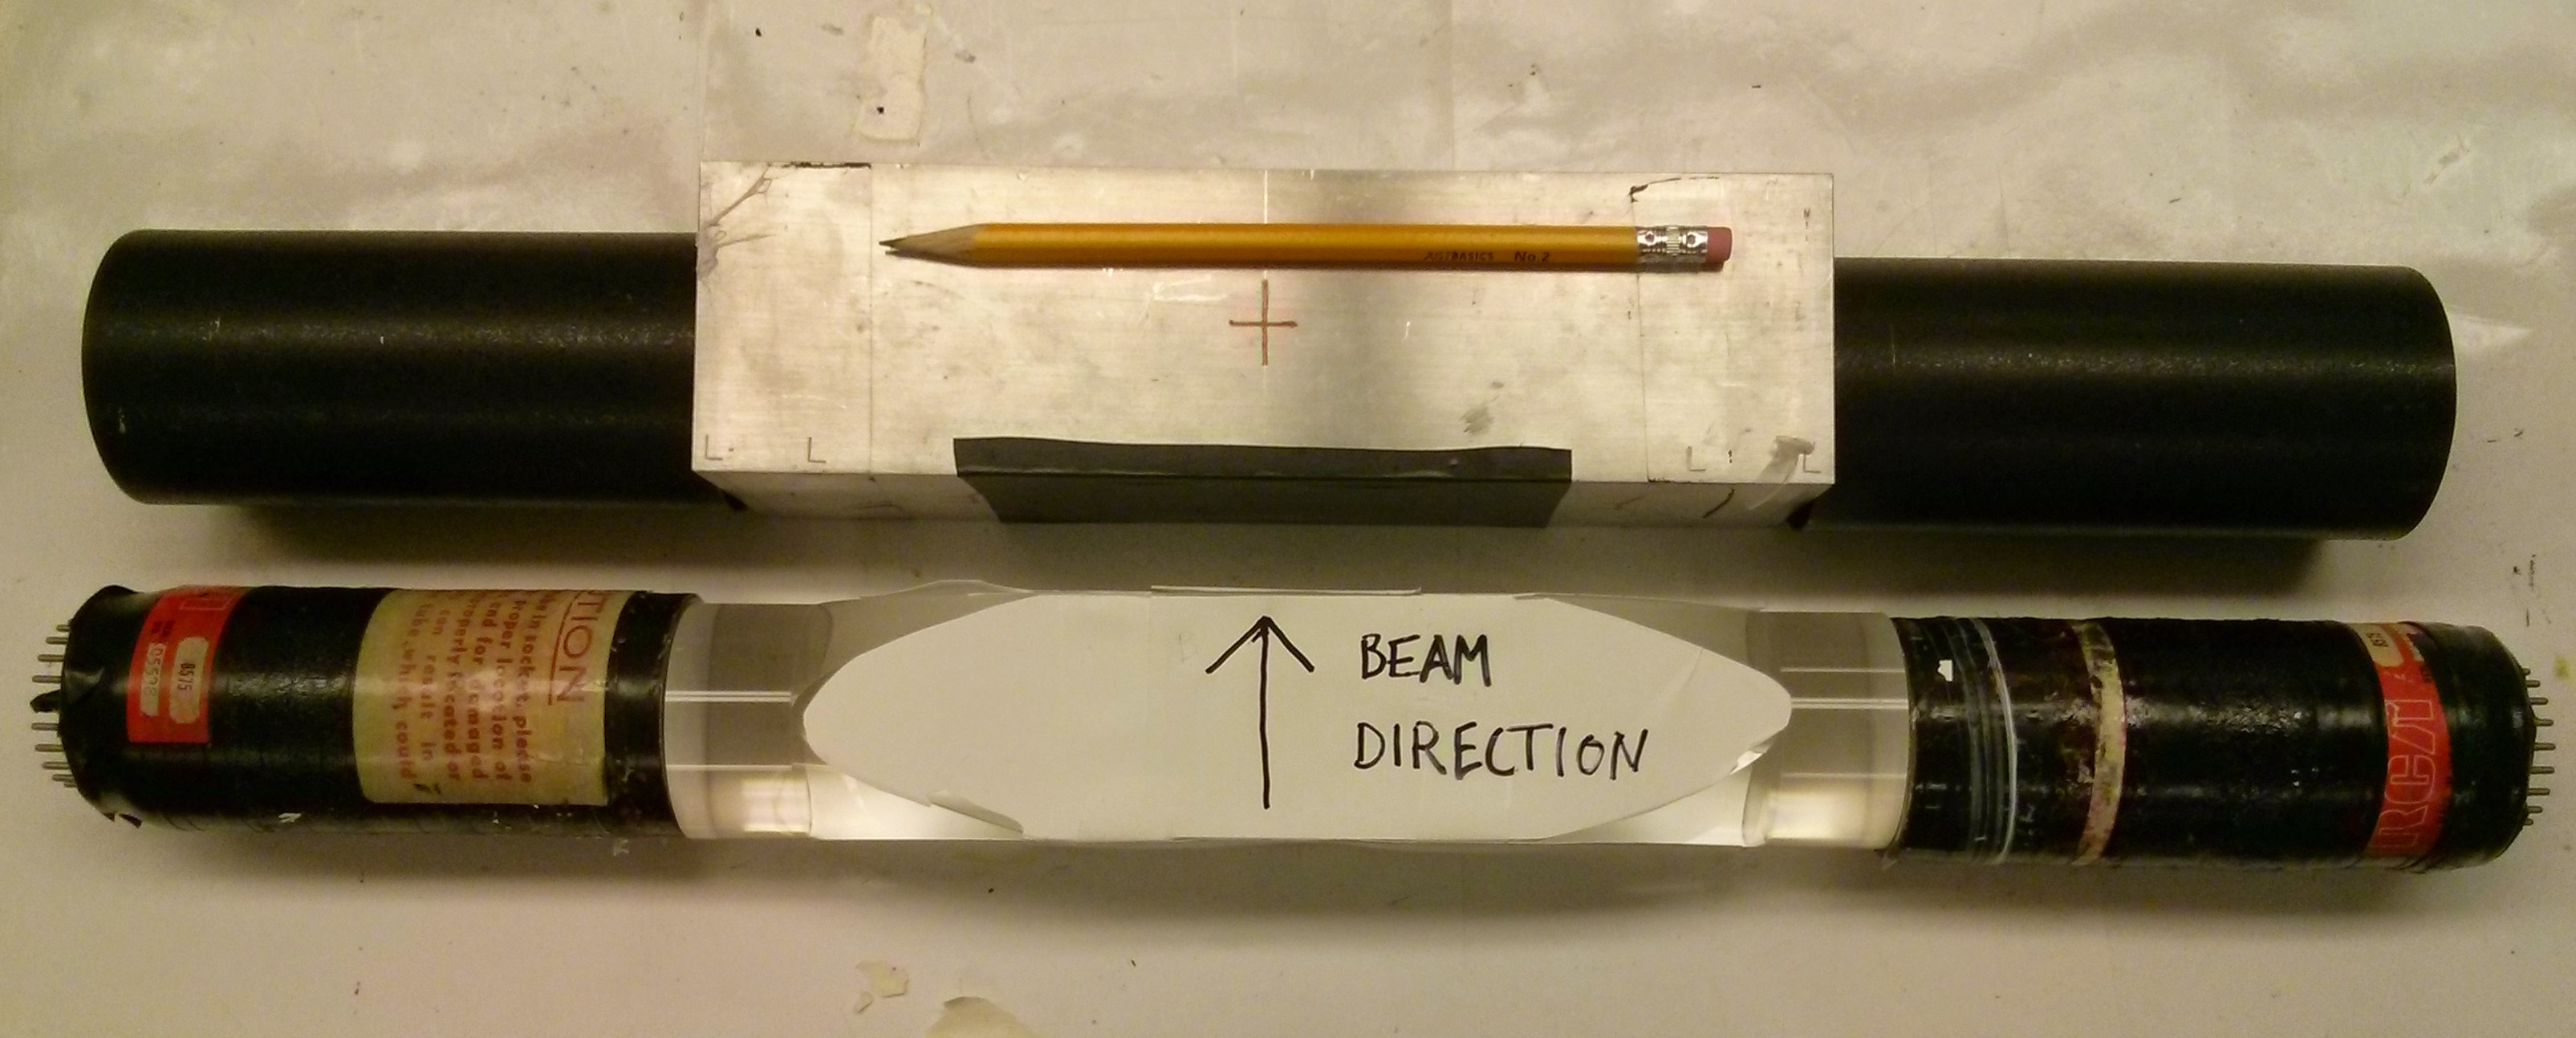
\includegraphics[width=0.8\textwidth]{figures/Scintillator_disassembled.jpg}
    \caption[TOF detector partially assembled]
    {One of three TOF detectors, partially assembled, with pencil for scale.
        The aluminum casing and Delrin phototube sleeves are at top, and the
        scintillator (beneath the beam direction arrow), lightguides, and phototubes, at
        bottom. The detector described in the text has a thinner scintillating plastic
    element (1 inch thick) and tapered lightguides to match.}
    \label{TOFDetectorDisassembled}
\end{figure}
\begin{figure}[tb]
    \centering
    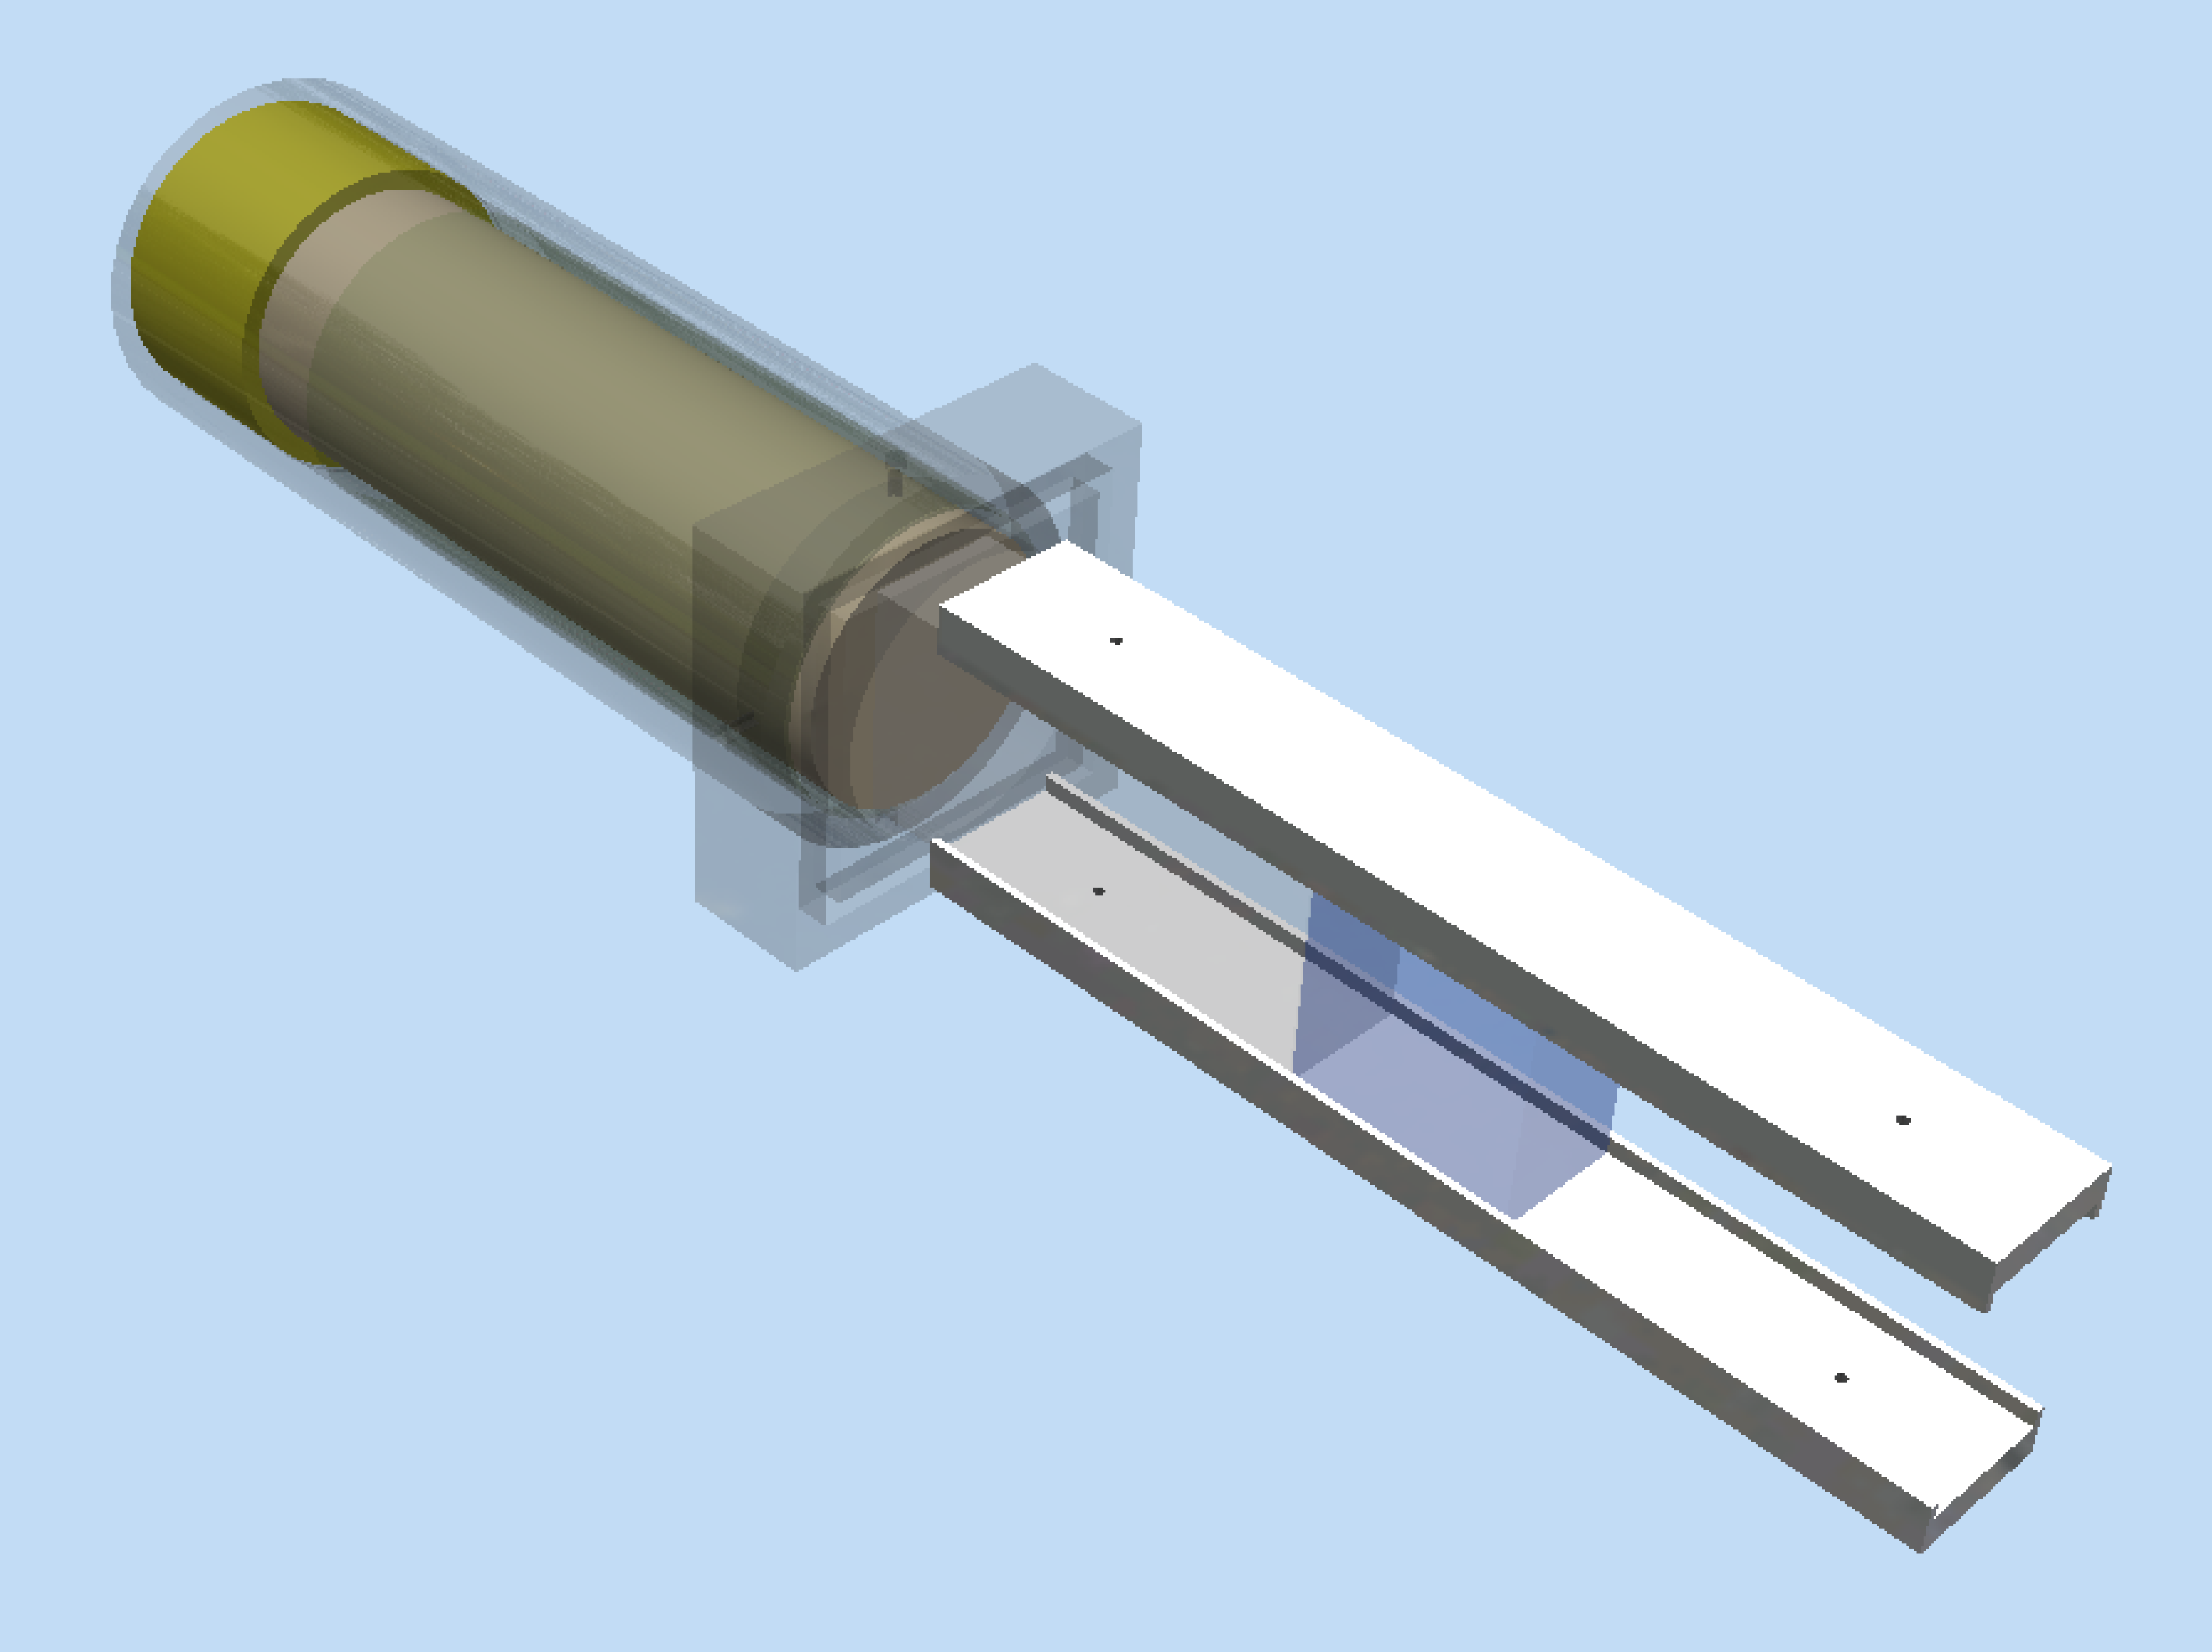
\includegraphics[width=0.8\textwidth]{figures/TimeOfFlightCAD.png}
    \caption[Cutaway CAD figure of TOF detector.]
    {
        Cutaway CAD figure of TOF detector described in the text. The 
        1-inch-thick scintillating plastic element is visible in the middle of the aluminum 
        housing brackets, and the light-tight sleeve for the phototube is visible on
        the left.
    }
    \label{TOFCAD}
\end{figure}

Figure \ref{TOFDetectorDisassembled} shows a TOF detector used in one
of our neutron \tot\ measurements. A 2-inch x 2-inch x 1-inch block of BC-400 fast
plastic scintillator is coupled to two transparent
BC-800 adiabatic lightguides with RTV rubberized adhesive. The 2-inch x 2-inch face is perpendicular
to the beam and the 1-inch dimension is parallel to the beam. These components were encased
in an aluminum structural housing. On the distal end of the lightguides, Hamamatsu 1668
photomultiplier tubes were connected with optical grease and enclosed by
$\upmu$-metal shielding, used to prevent external magnetic fields from affecting photoelectrons.
Phototube signals and high voltage were supplied by a phototube base attached to the back of each
phototube. To hold the phototubes, fitted black Delrin sleeves (shown on the
left side of the CAD cutaway Fig. \ref{TOFCAD}) were custom-made to apply slight
compression, keeping the optical surfaces in good contact. The entire assembly
is 24 9/16 inch in length.

\section{Sample Preparation}
Where possible, the \tot\ samples were formed as right
cylinders 8.25 mm in diameter and ranging from 10-27 mm in length (see
Table \ref{SampleCharacteristics} for sample characteristics and Fig. \ref{SamplesImage}
for sample images). A natural-abundance sample
was also prepared for each element for use in benchmarking to already-existing
literature neutron \tot\ values. During the experiment, the samples were inserted
into styrofoam sleeves and seated in the cradles of the sample
changer, described below. This design minimizes the amount of non-target mass proximate to the
neutron beam path that could cause unwanted neutron scattering. The areal density of atoms,
the relevant quantity for cross section measurements, for each O, Ni, and Sn sample differs by less 
than 1\% compared to the other samples of the same element.
\begin{table}[tb]
    \caption[Physical characteristics of samples used for neutron \tot\
    measurements]
    {
        For isotopically-enriched samples, the natural abundance
        of the enriched isotope and the isotopic fraction of the sample are
        given. To calculate cross sections, the relevant ``sample thickness'' is the areal
        density of nuclei $\rho_{\text{areal}}$, equivalent to
        the (volumetric) density times the length of the sample. For liquid
        samples H$_{2}^{\text{nat}}$O, D$_{2}^{\text{nat}}$O, and H$_{2}^{18}$O,
        the length and diameter listed are for the interior of the vessels
        used to hold the samples and the masses given are calculated based on 
        literature values for the density of each sample at 25\textdegree{}C.
        Our samples are generally much smaller than those used in previous
        measurements; for comparison, the Ni and Sn samples used in \cite{Abfalterer2001,
        Finlay1993} had areal densities of 1.515 and 0.5475
        $\frac{mol}{cm^{2}}$, respectively (12.7 and 6.5 times larger than our
        Ni and Sn samples). Columns 6 and 7 give the natural abundance of the
        isotope (NA) and the purity of our isotopic samples (SP).
    }
    \label{SampleCharacteristics}
    \begin{center}
        \begin{tabular}{ c c c c c c c }
            \toprule
            Isotope & Len. [\milli\meter] & Diam. [\milli\meter]
            & Mass [\gram] & $\rho_{\text{areal}}$
            [$\frac{mol}{cm^{2}}$] & NA [\%] & SP 
            [\%]\\
            \midrule

            $^{\text{nat}}$C & 13.66(2) & 8.260(5) & 1.2363
            & 0.1921(1) & - & -\\
            $^{\text{nat}}$C & 27.29(2) & 8.260(5) & 2.4680
            & 0.3835(2) & - & -\\
            \\
            H$_{2}$$^{\text{nat}}$O & 20.00(1) & 8.92(1) & 1.2461 & 0.1107(3) & - &
            - \\
            D$_{2}$$^{\text{nat}}$O & 20.00(1) & 8.92(1) & 1.3852 & 0.1107(3) & - &
            - \\
            H$_{2}$$^{18}$O & 20.00(1) & 8.92(1) & 1.3844 & 0.1107(3) & 0.20 & 99\\
            \\
            $^{58}$Ni & 7.97(3)& 8.18(2) &
            3.6438 & 0.1197(3)& 68.1 & 99.6 \\
            $^{\text{nat}}$Ni & 8.00(3) & 8.20(2) &
            3.6898 & 0.1192(3)& - & -\\
            $^{64}$Ni & 7.96(2) & 8.20(4) &
            3.9942 & 0.1192(6) & 0.93 & 92.2\\
            \\
            $^{103}$Rh & 2.03(1) & 10.20(2) & 2.8359 & 0.02426(4) & 100 & 99.9\\
            \\
            $^{112}$Sn & 13.65(3) & 8.245(5) &
            4.9720 & 0.08332(5) & 0.97 & 99.9\\
            $^{\text{nat}}$Sn & 13.68(3) & 8.245(5) &
            5.3263 & 0.08414(5) & - & -\\
            $^{124}$Sn & 13.73(3) & 8.245(5) &
            5.5492 & 0.08399(5) & 5.79 & 99.9\\
            \\
            $^{\text{nat}}$Pb & 10.07(2) & 8.27(1) & 6.130 &
            0.05508(6) & - & -\\
            \bottomrule
        \end{tabular}
    \end{center}
\end{table}
\begin{figure}[tb]
    \centering
    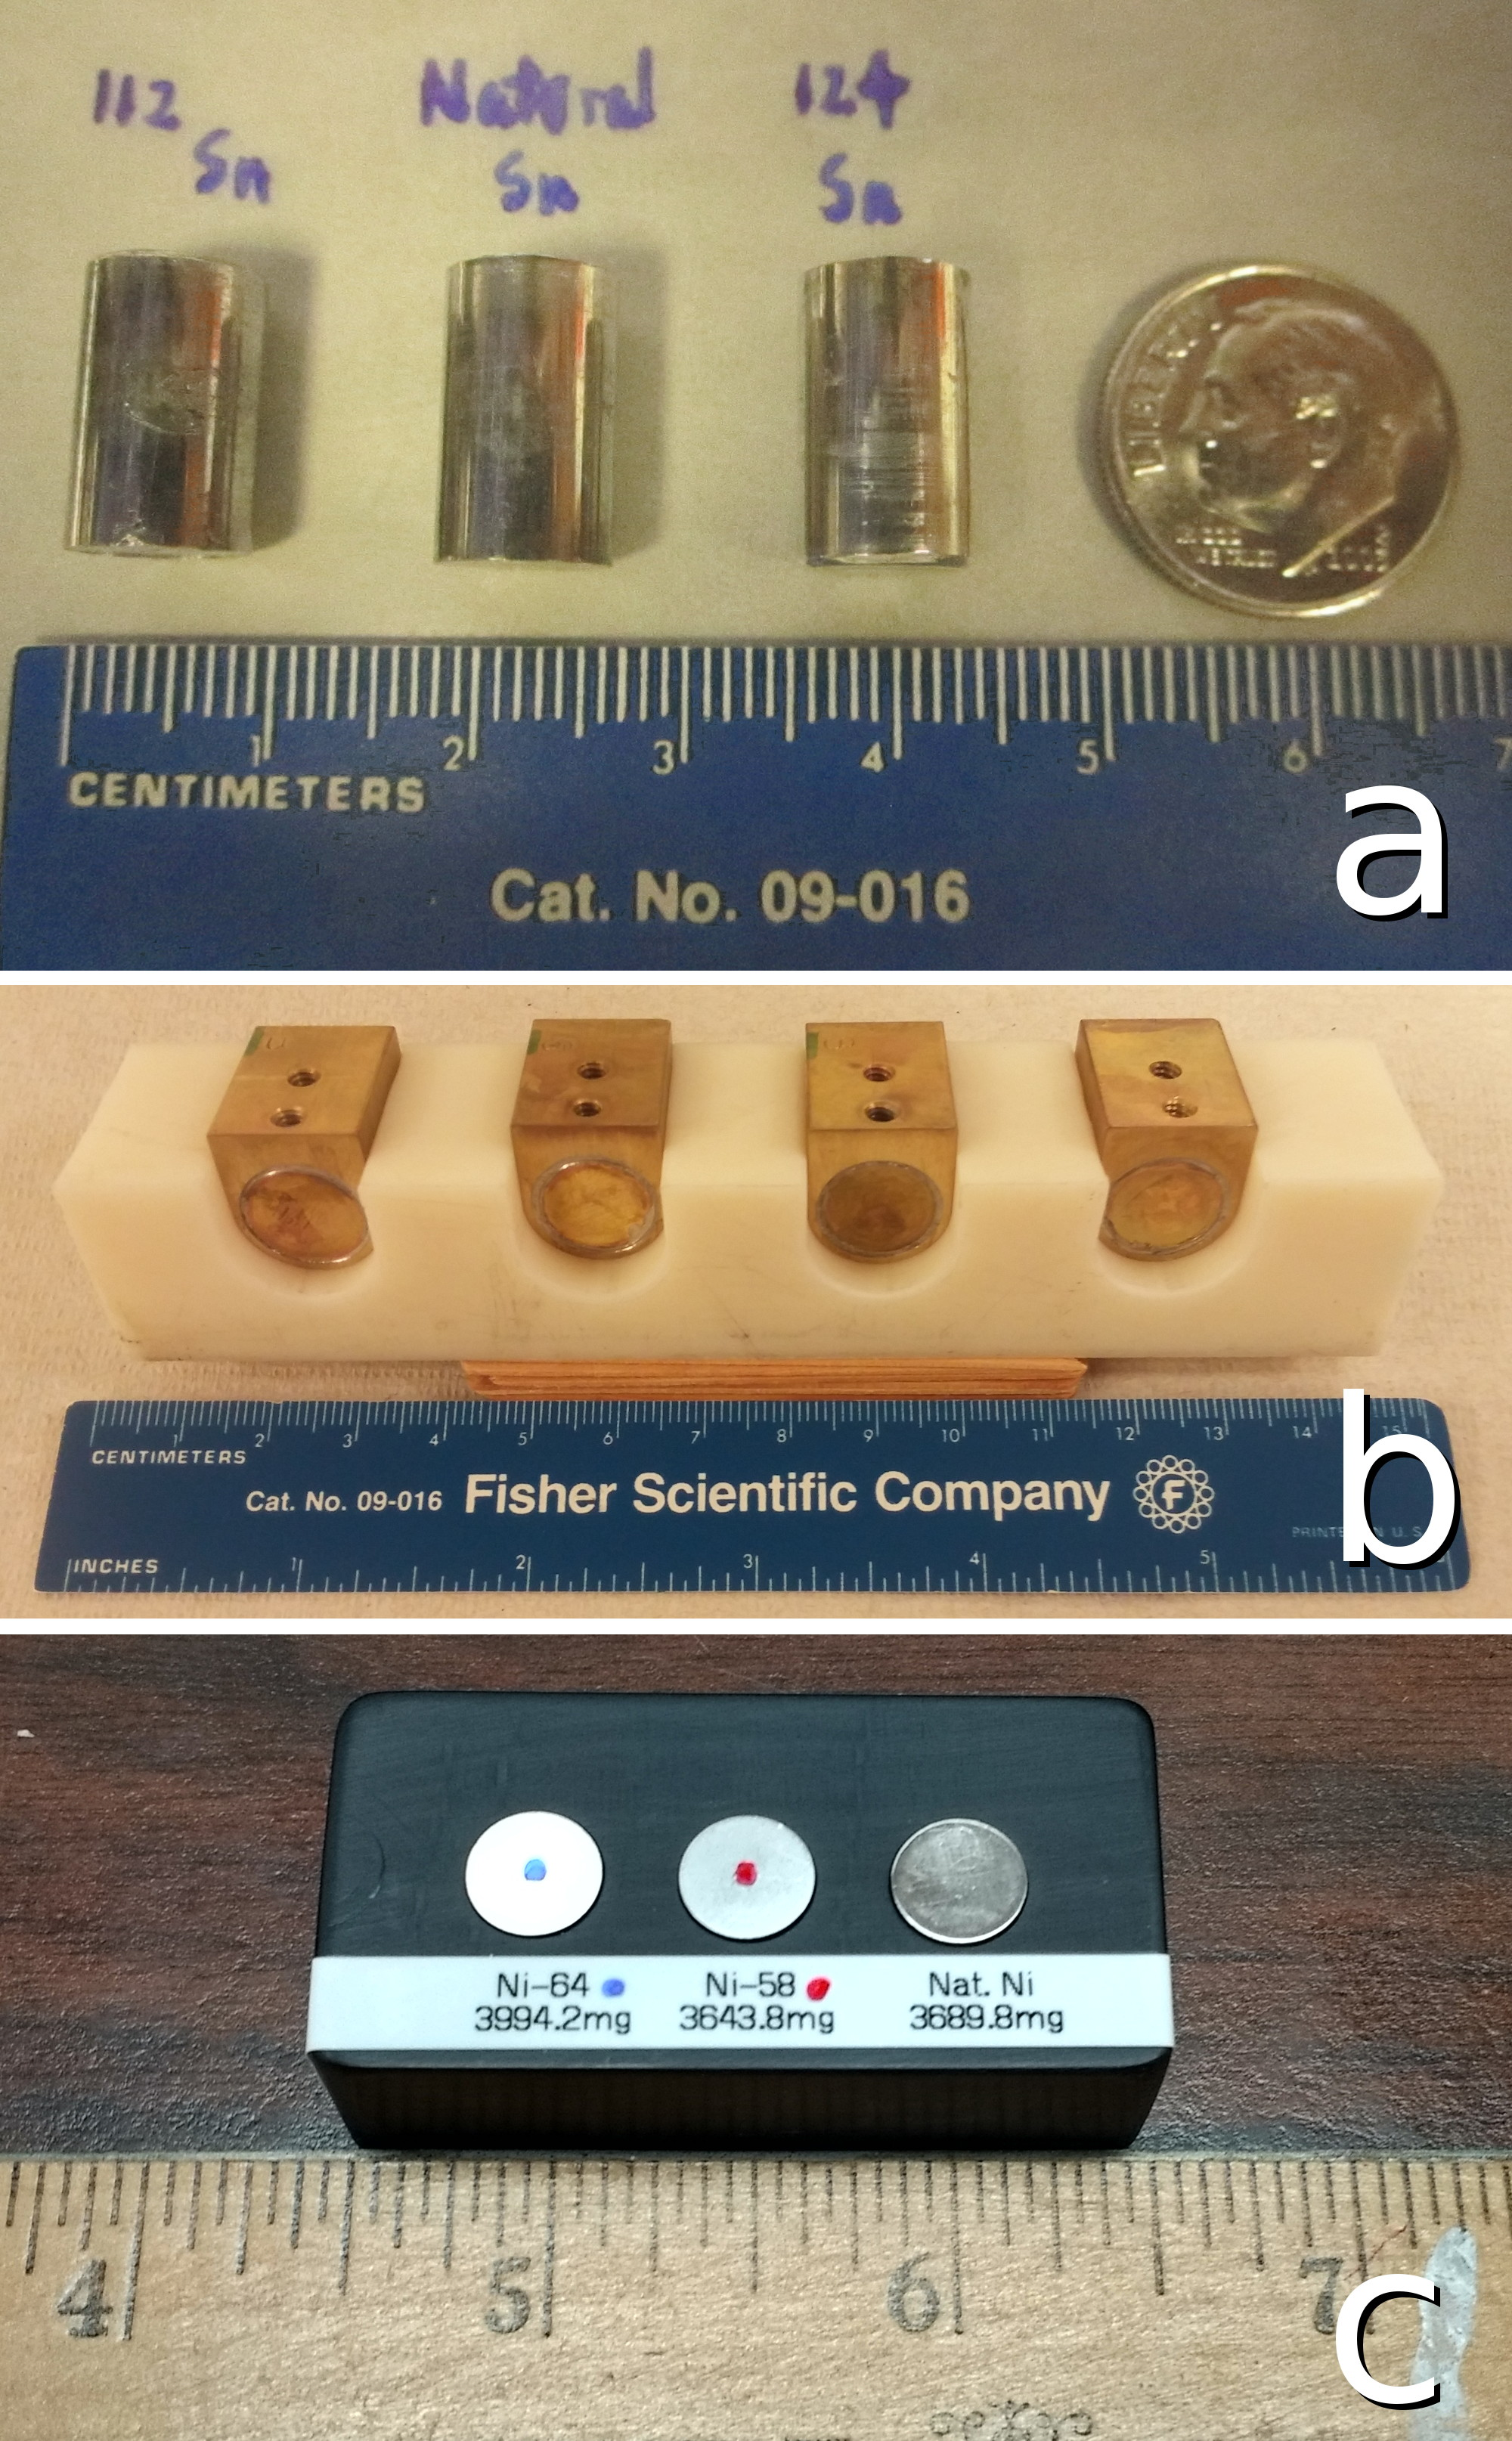
\includegraphics[width=0.7\textwidth]{figures/AllIsotopicSamples.jpg}
    \caption[${^{112,\text{nat},124}}$Sn, $^{{\text{nat}, 18}}$O, and ${^{58,\text{nat},64}}$Ni
    samples used for neutron \tot\ measurements]
    {
        ${^{112,\text{nat},124}}$Sn (section a), H$_2^{{\text{nat}, 18}}$O (section
        b), and ${^{58,\text{nat},64}}$Ni
        samples (section c) used for neutron \tot\ measurements, with rulers for
        scale. Brass vessels were used to hold the water samples.
    }
    \label{SamplesImage}
\end{figure}

\begin{figure}[tb]
    \centering
    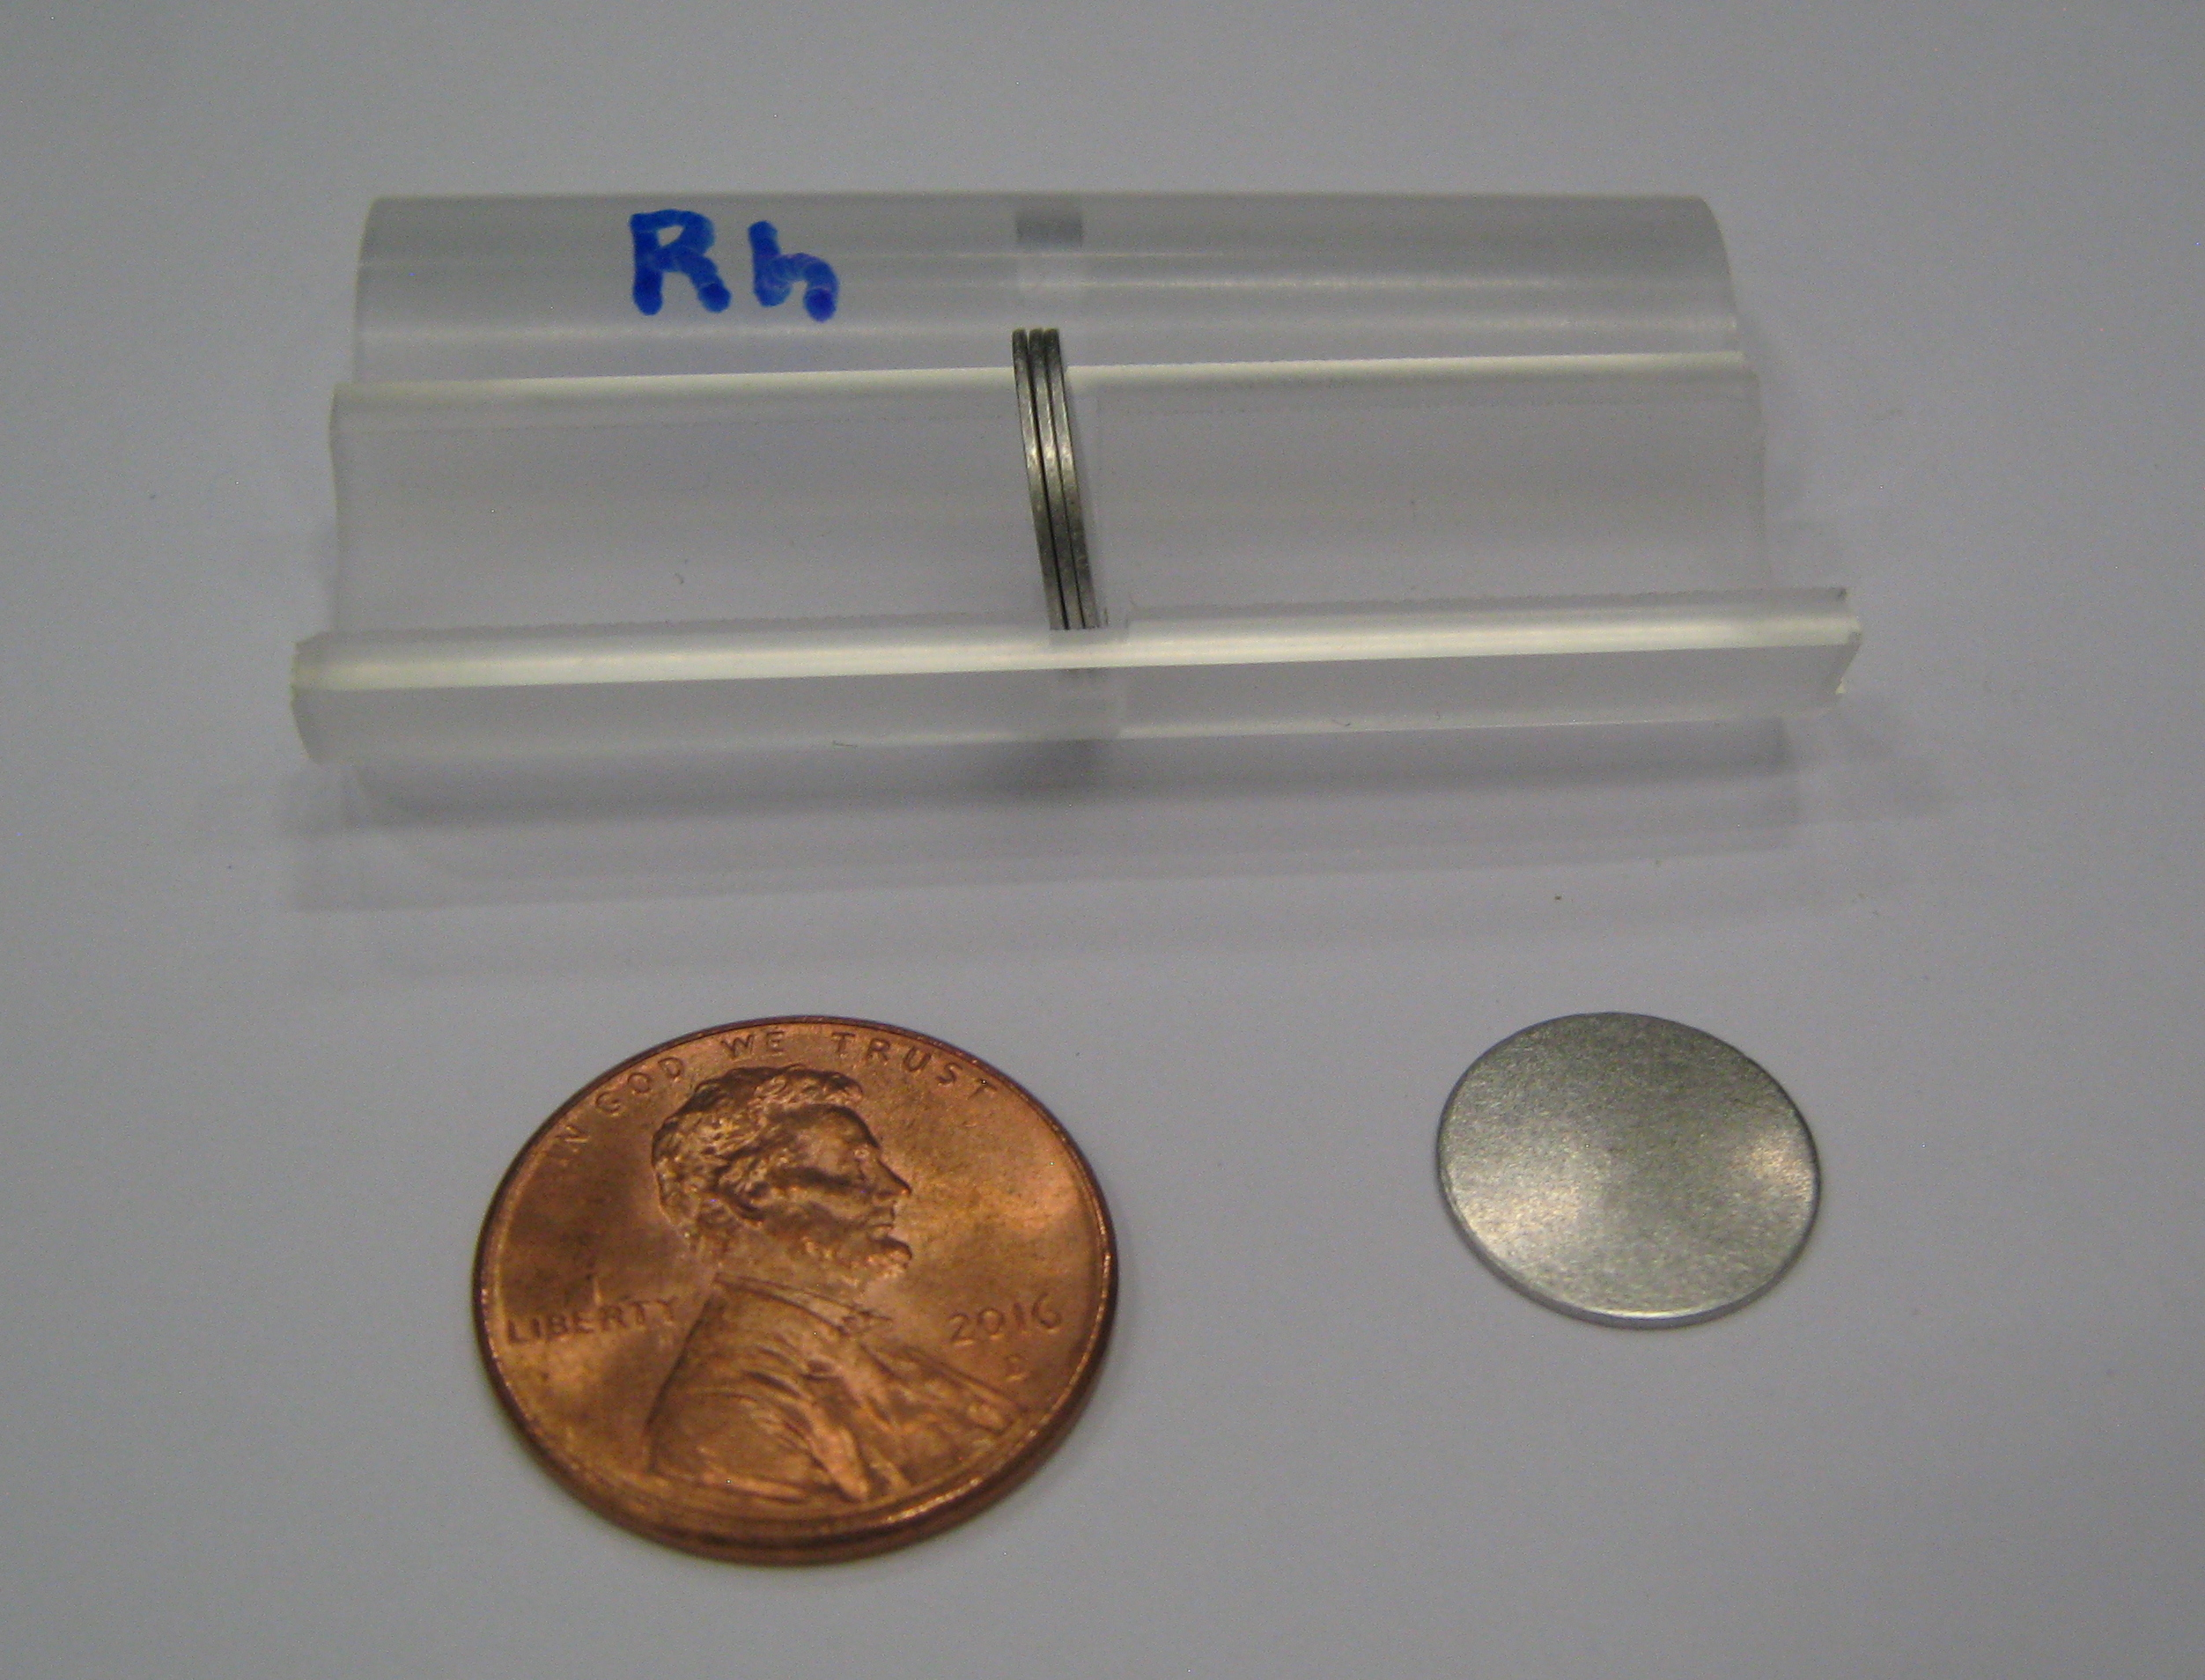
\includegraphics[width=0.8\textwidth]{figures/RhodiumSample.jpg}
    \caption[\rhThree\ sample used for the neutron \tot\ measurements]
    {\rhThree\ sample used for the neutron \tot\ measurements. One of
    the four Rh discs has been removed from the plastic sleeve to show detail.}
    \label{RhodiumSample}
\end{figure}

For the oxygen isotopes, isotopically-enriched water samples were prepared to
increase the areal density of O in the sample volume and for ease of handling.
After measurement, the
extremely-well-known H neutron \tot\ could be subtracted to yield the O \tot\ values.
This technique is also used by \cite{Vaughn1965, Salisbury1965}; cf. 
the use of ZnO and BeO \cite{Finlay1993}.
Because the natural abundance of \oSix\ in H$_{2}$O is $>$99\%, a sample of
ordinary distilled water was used for the H$_{2}$\oSix\ sample. For H$_{2}$\oEight,
we used distilled water enriched to 99.9\% in \oEight\, purchased from
Aldrich. Both samples were enclosed in brass vessels with thin
(0.002 inch) brass endcaps, to minimize neutron attenuation. At the temperature and
altitude of the experimental facility, the amount of dissolved gas and ions
in the water samples were small enough to have no effect on the measurement.

The isotopic Sn samples were prepared by melting highly-enriched foils at 
800 C in a tube furnace, cooling to ambient temperature, and pressing the ingots
to the desired cylindrical shape in a tempered die. To reduce formation of tin
oxide during melting, the samples were melted in vitreous carbon crucibles
and kept under a reducing atmosphere (90\% Argon/10\% H$_{2}$) while at elevated
temperatures. Of the 4.9 grams of \snTwelve\ used to prepare the sample,
3.9 grams were from a semi-permanent loan from the group of Lee Bernstein from LLNL
and the remainder we purchased from Isoflex Corp. All of the 5.8 grams of \snFour\
were purchased from Isoflex. The \snNat\ sample was prepared by melting and
pressing analytical-grade Sn shot from Mallinckrodt Corp. Loss of isotopic
material during the sample preparation process was minimal.
The natural and isotopic Ni samples were 
prepared by Mike Zach at Oak Ridge National Lab (ORNL) to match the diameter of our Sn samples.

Due to its poor machining properties, the Rh sample was prepared by
stacking a series of thin rhodium disks instead of manufacturing a
fused cylinder. Four disks of 99.9\% pure natural (monoisotopic) Rh metal were purchased from
Goodfellow Corp. These were corralled with a
plastic sleeve with open ends, similar to the styrofoam sleeves used for the Ni
and Sn samples, to match the $\frac{3}{4}$-inch-diameter cradles of the sample changer
\ref{RhodiumSample}.
This kept the discs snugly in series and perpendicular to the beam path.

Lastly, two natural-abundance graphite samples of different lengths and one
natural-abundance Pb sample, all with the same diameter as the Sn and Ni samples, were
prepared. These samples were used to benchmark the total cross sections
measured at LANSCE by comparison with previous measurements of the C and
Pb total cross sections available in the literature
\cite{Finlay1993,Abfalterer2001}. In addition, the low-energy neutron \tot\ resonance
structure of the C samples served a crucial role in fixing the exact distance
of the TOF detector as detailed in Chapter \ref{TCSAnalysis}.
Before use, the C samples were baked in an oven for several
hours to remove adsorbed water.

Appendix \ref{SampleComposition} lists the full composition of each isotopic
sample as listed by the manufacturer or from mass spectrometer analysis.

\section{Experimental Facility at LANSCE}
All neutron \tot\ measurements were carried out at the 15R
beamline of the Weapons Neutron Research (WNR) facility at the Los Alamos
Neutron Science Center (LANSCE) over two run cycles (November 2016 and
September 2017). At WNR, broad-spectrum neutrons up
to 800 \mega\electronvolt\ are generated by impinging proton beam onto a water-cooled, 7.5-cm-long
tungsten target (see Fig. \ref{ExperimentalApparatus}). A 
permanent magnet deflects all charged particles from the beam path, 
allowing only neutrons and $\gamma$ rays to reach our samples. Neutron flux can be
adjusted by the user with a pair of horizontal and vertical shutters upstream of the
experimental vault. Based on beam divergence
simulations, the beam was collimated to 0.200 inch at the entrance to the
experimental vault using steel donuts with a total thickness of 24 inch.
To reduce (but not eliminate) the $\gamma$-ray component of the beam,
a $\frac{1}{2}$-inch plug of Hevimet (90\% W, 6\% 
Ni, 4\% Cu by weight) was inserted at the upstream end of the
stack of collimator donuts. After collimation, the beam passed successively through a flux 
monitor, the sample of interest held in a sample changer (see Fig.
\ref{BeamlineSampleChanger}), a veto detector, and finally the 
TOF detector approximately 25 meters from the neutron source (see Fig.
\ref{VetoAndTOFDetectors}). The monitor detector and veto detector
were constructed along similar principles to the TOF
detector construction but only have one phototube each. The monitor and
veto detectors each had scintillator thicknesses of $\frac{1}{4}$ inch.
Figure \ref{BeamlineUpstream} shows the entire experimental area, looking upstream
from the perspective of the TOF
detector. Figure \ref{BeamlineDownstream} shows the same area, but looking
downstream from the monitor detector.
\begin{figure}[tb]
    \centering
    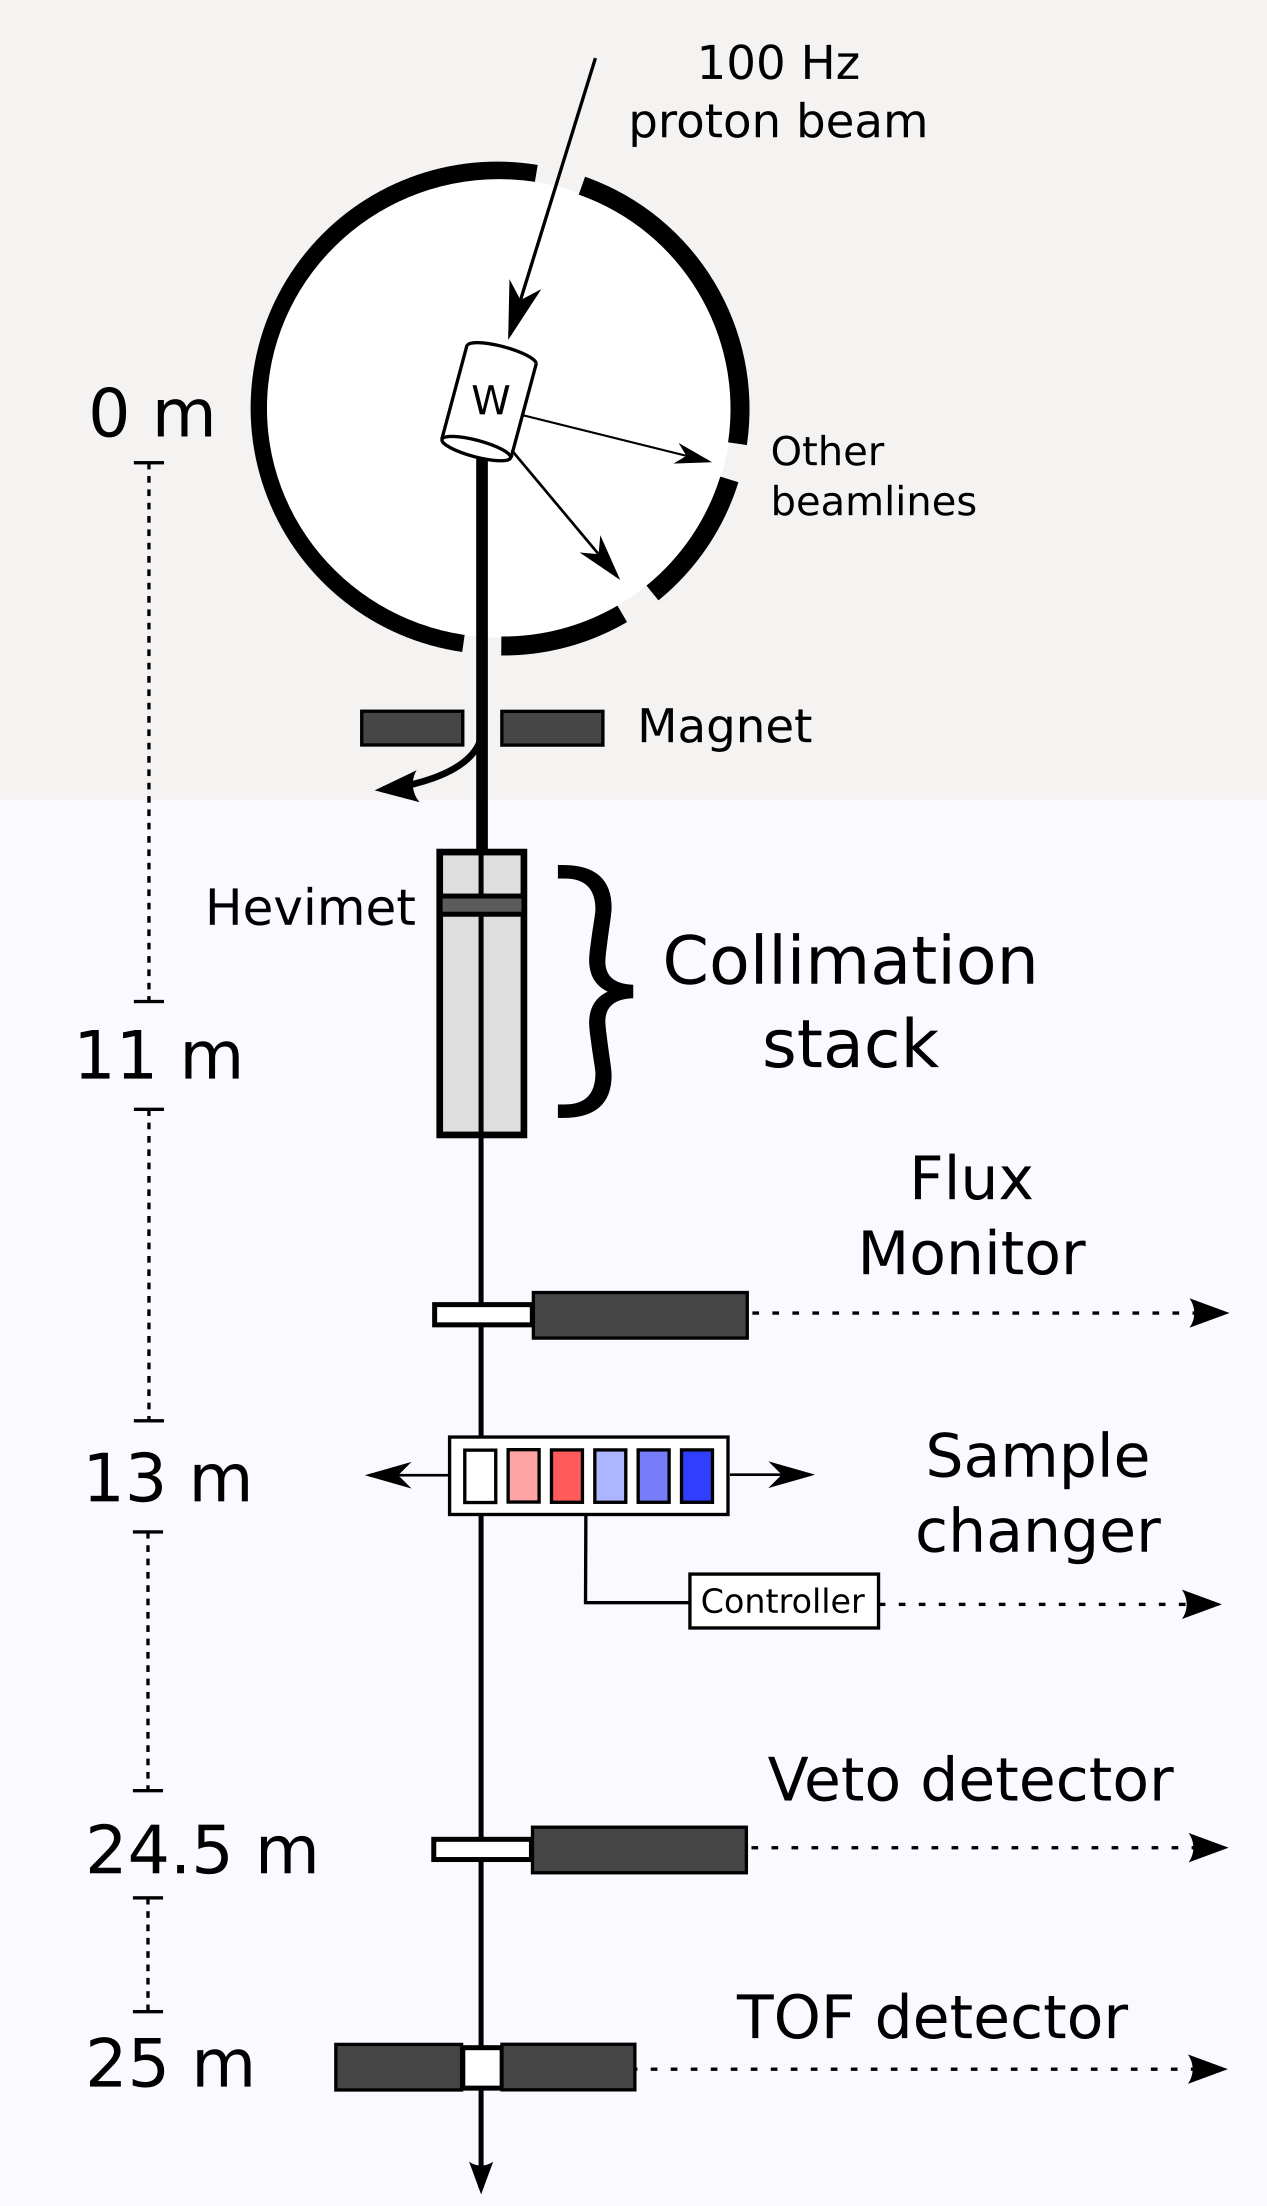
\includegraphics[height=0.7\textheight]{figures/ExperimentalSetup.png}
    \caption[Layout of the 15R beamline at the WNR facility at LANSCE]
    {Layout of the 15R beamline at the WNR facility at LANSCE, with our
        experimental equipment indicated toward the bottom of the flight path.
        After a permanent magnet sweeps charged particles from the beam, neutrons and
        $\gamma$-rays are collimated to 0.200 inch en route to the
        detectors used in the experiment. Samples are cycled into and out of beam
        using a linear actuator with a period of 150 seconds. Times-of-flight (TOFs) are
        determined by the TOF detector and used to calculate neutron energy.
    }
    \label{ExperimentalApparatus}
\end{figure}
\begin{figure}[tb]
    \centering
    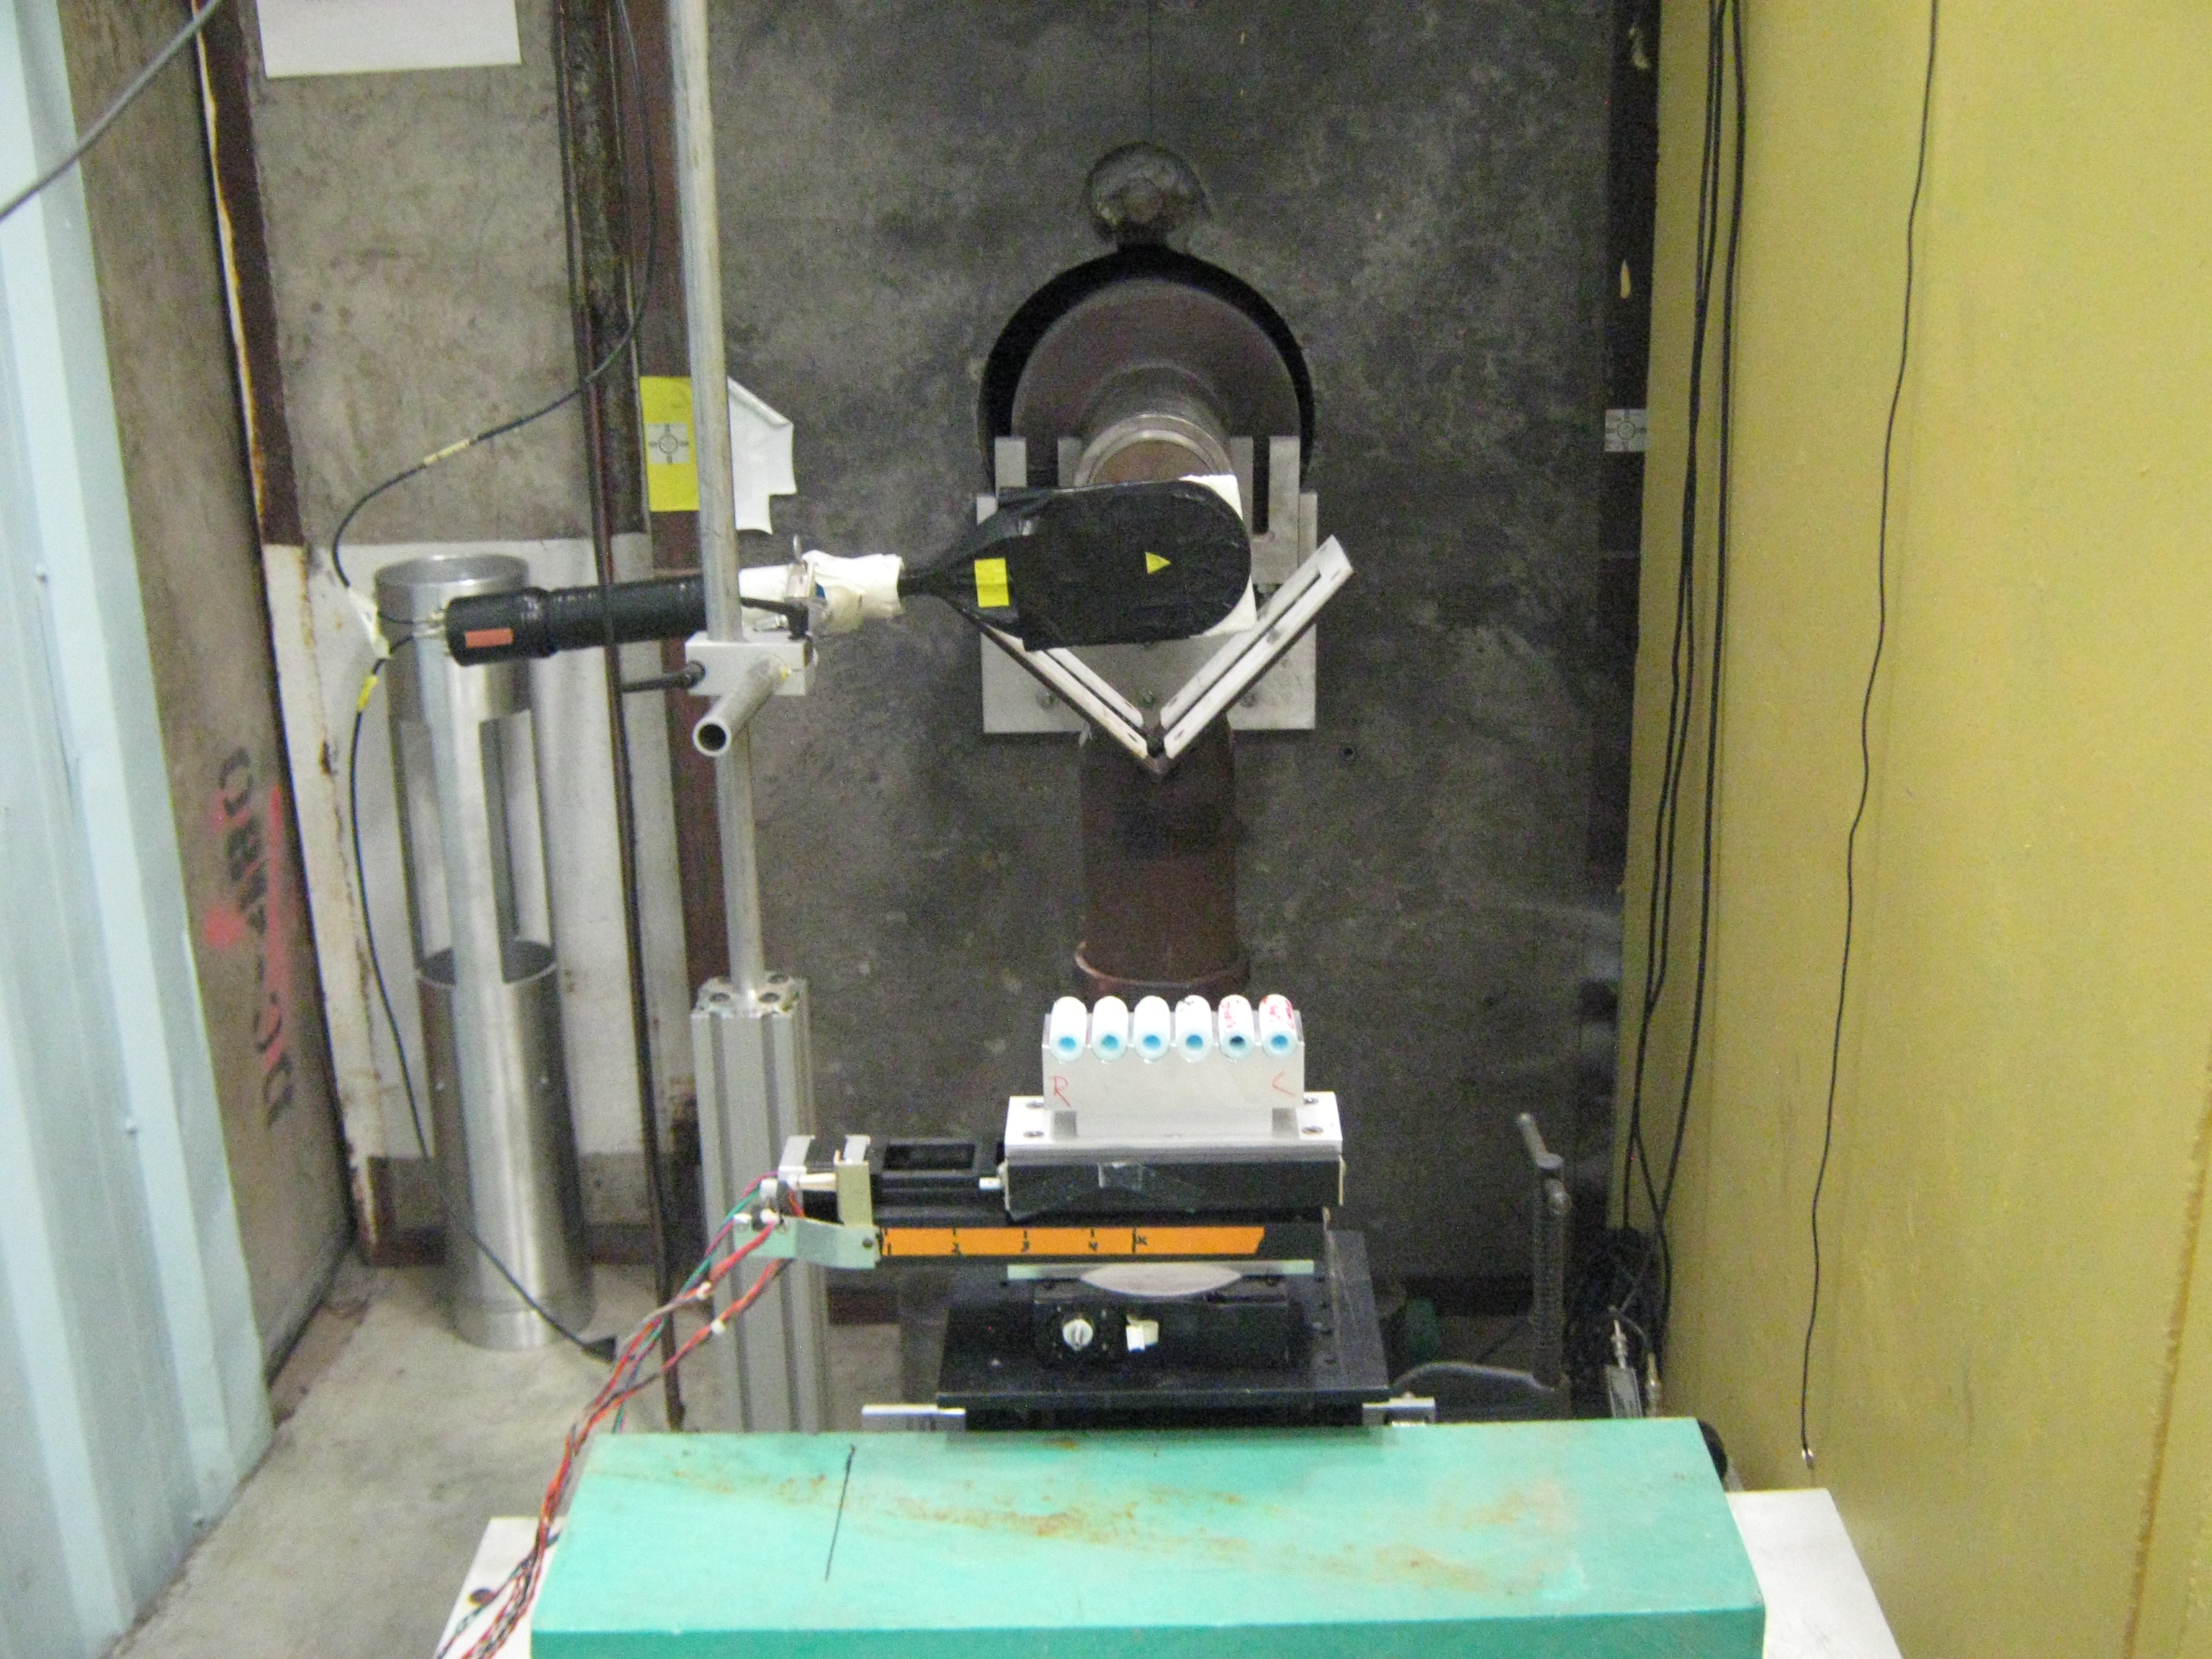
\includegraphics[width=0.9\textwidth]{figures/UpstreamTowardCollimator.jpg}
    \caption[Sample changer, monitor detector, and collimation stack]
    {Upstream view of sample changer, monitor detector, and collimation stack.}
    \label{BeamlineSampleChanger}
\end{figure}
\begin{figure}[tb]
    \centering
    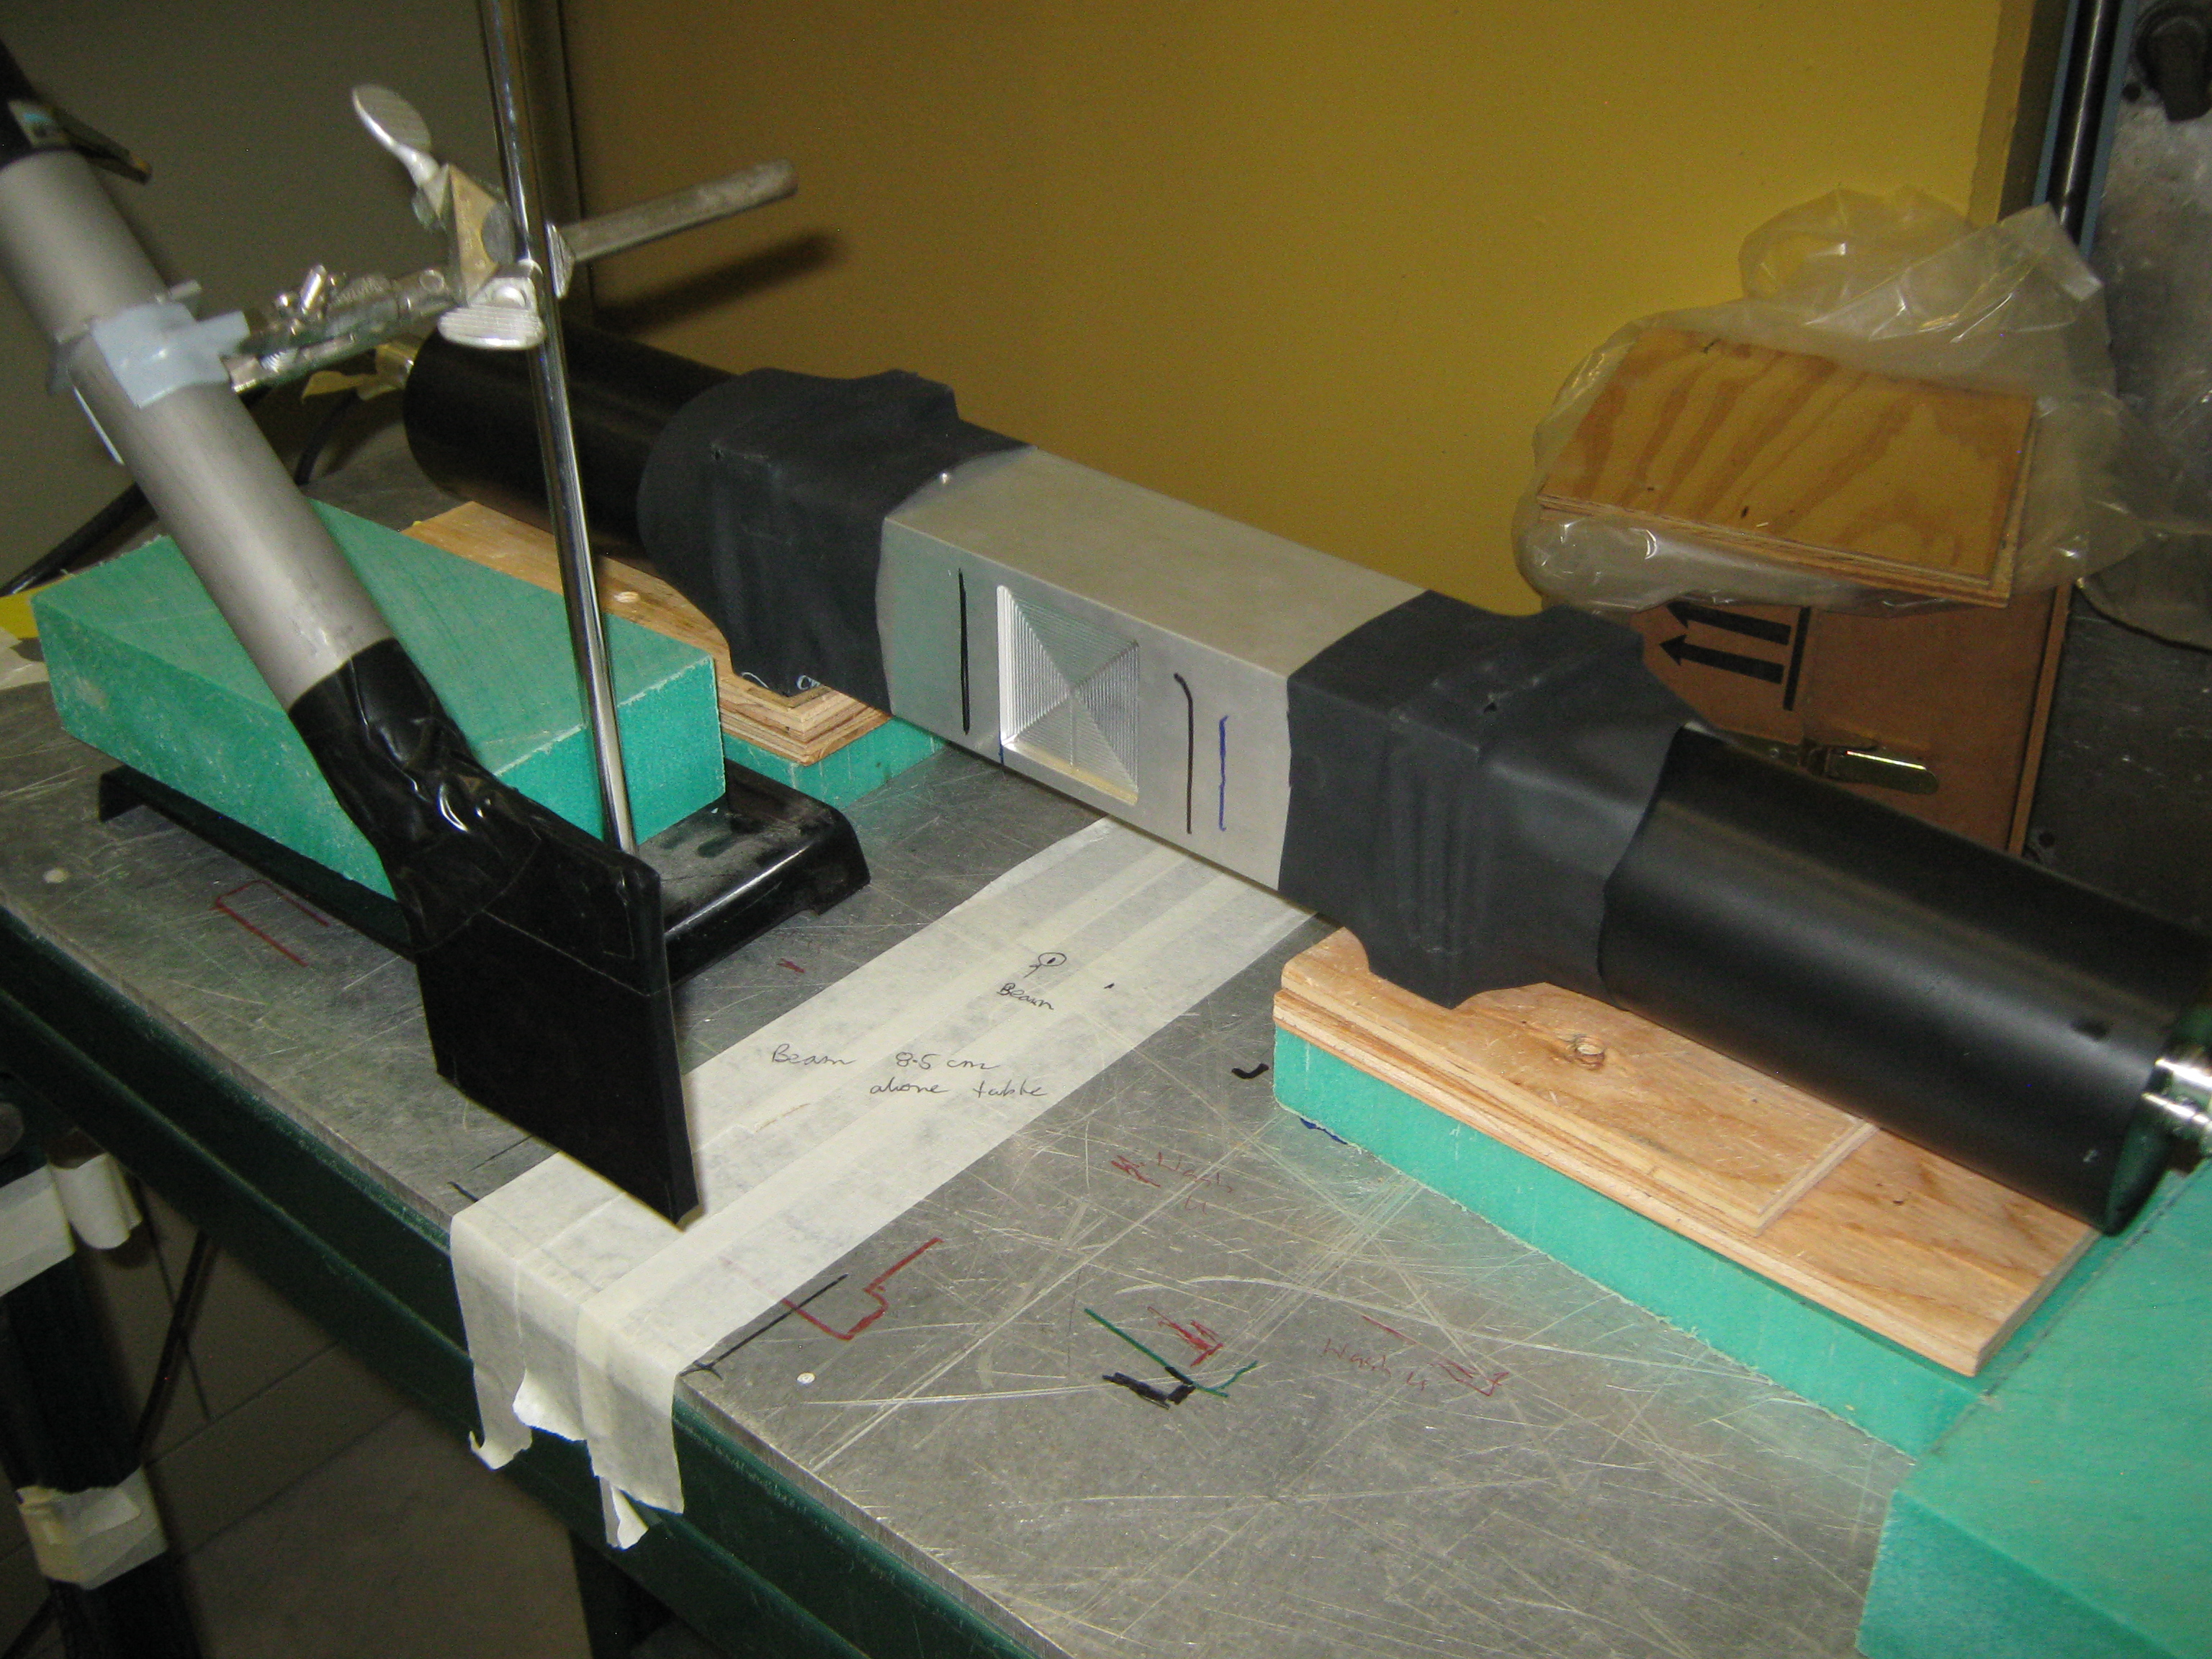
\includegraphics[width=0.9\textwidth]{figures/VetoAndTOFDetectors.jpg}
    \caption[Veto and TOF detectors installed in the 15R beamline]
    {Veto and TOF detectors installed in the 15R beamline. Beam enters from the left.}
    \label{VetoAndTOFDetectors}
\end{figure}
\begin{figure}[tb]
    \centering
    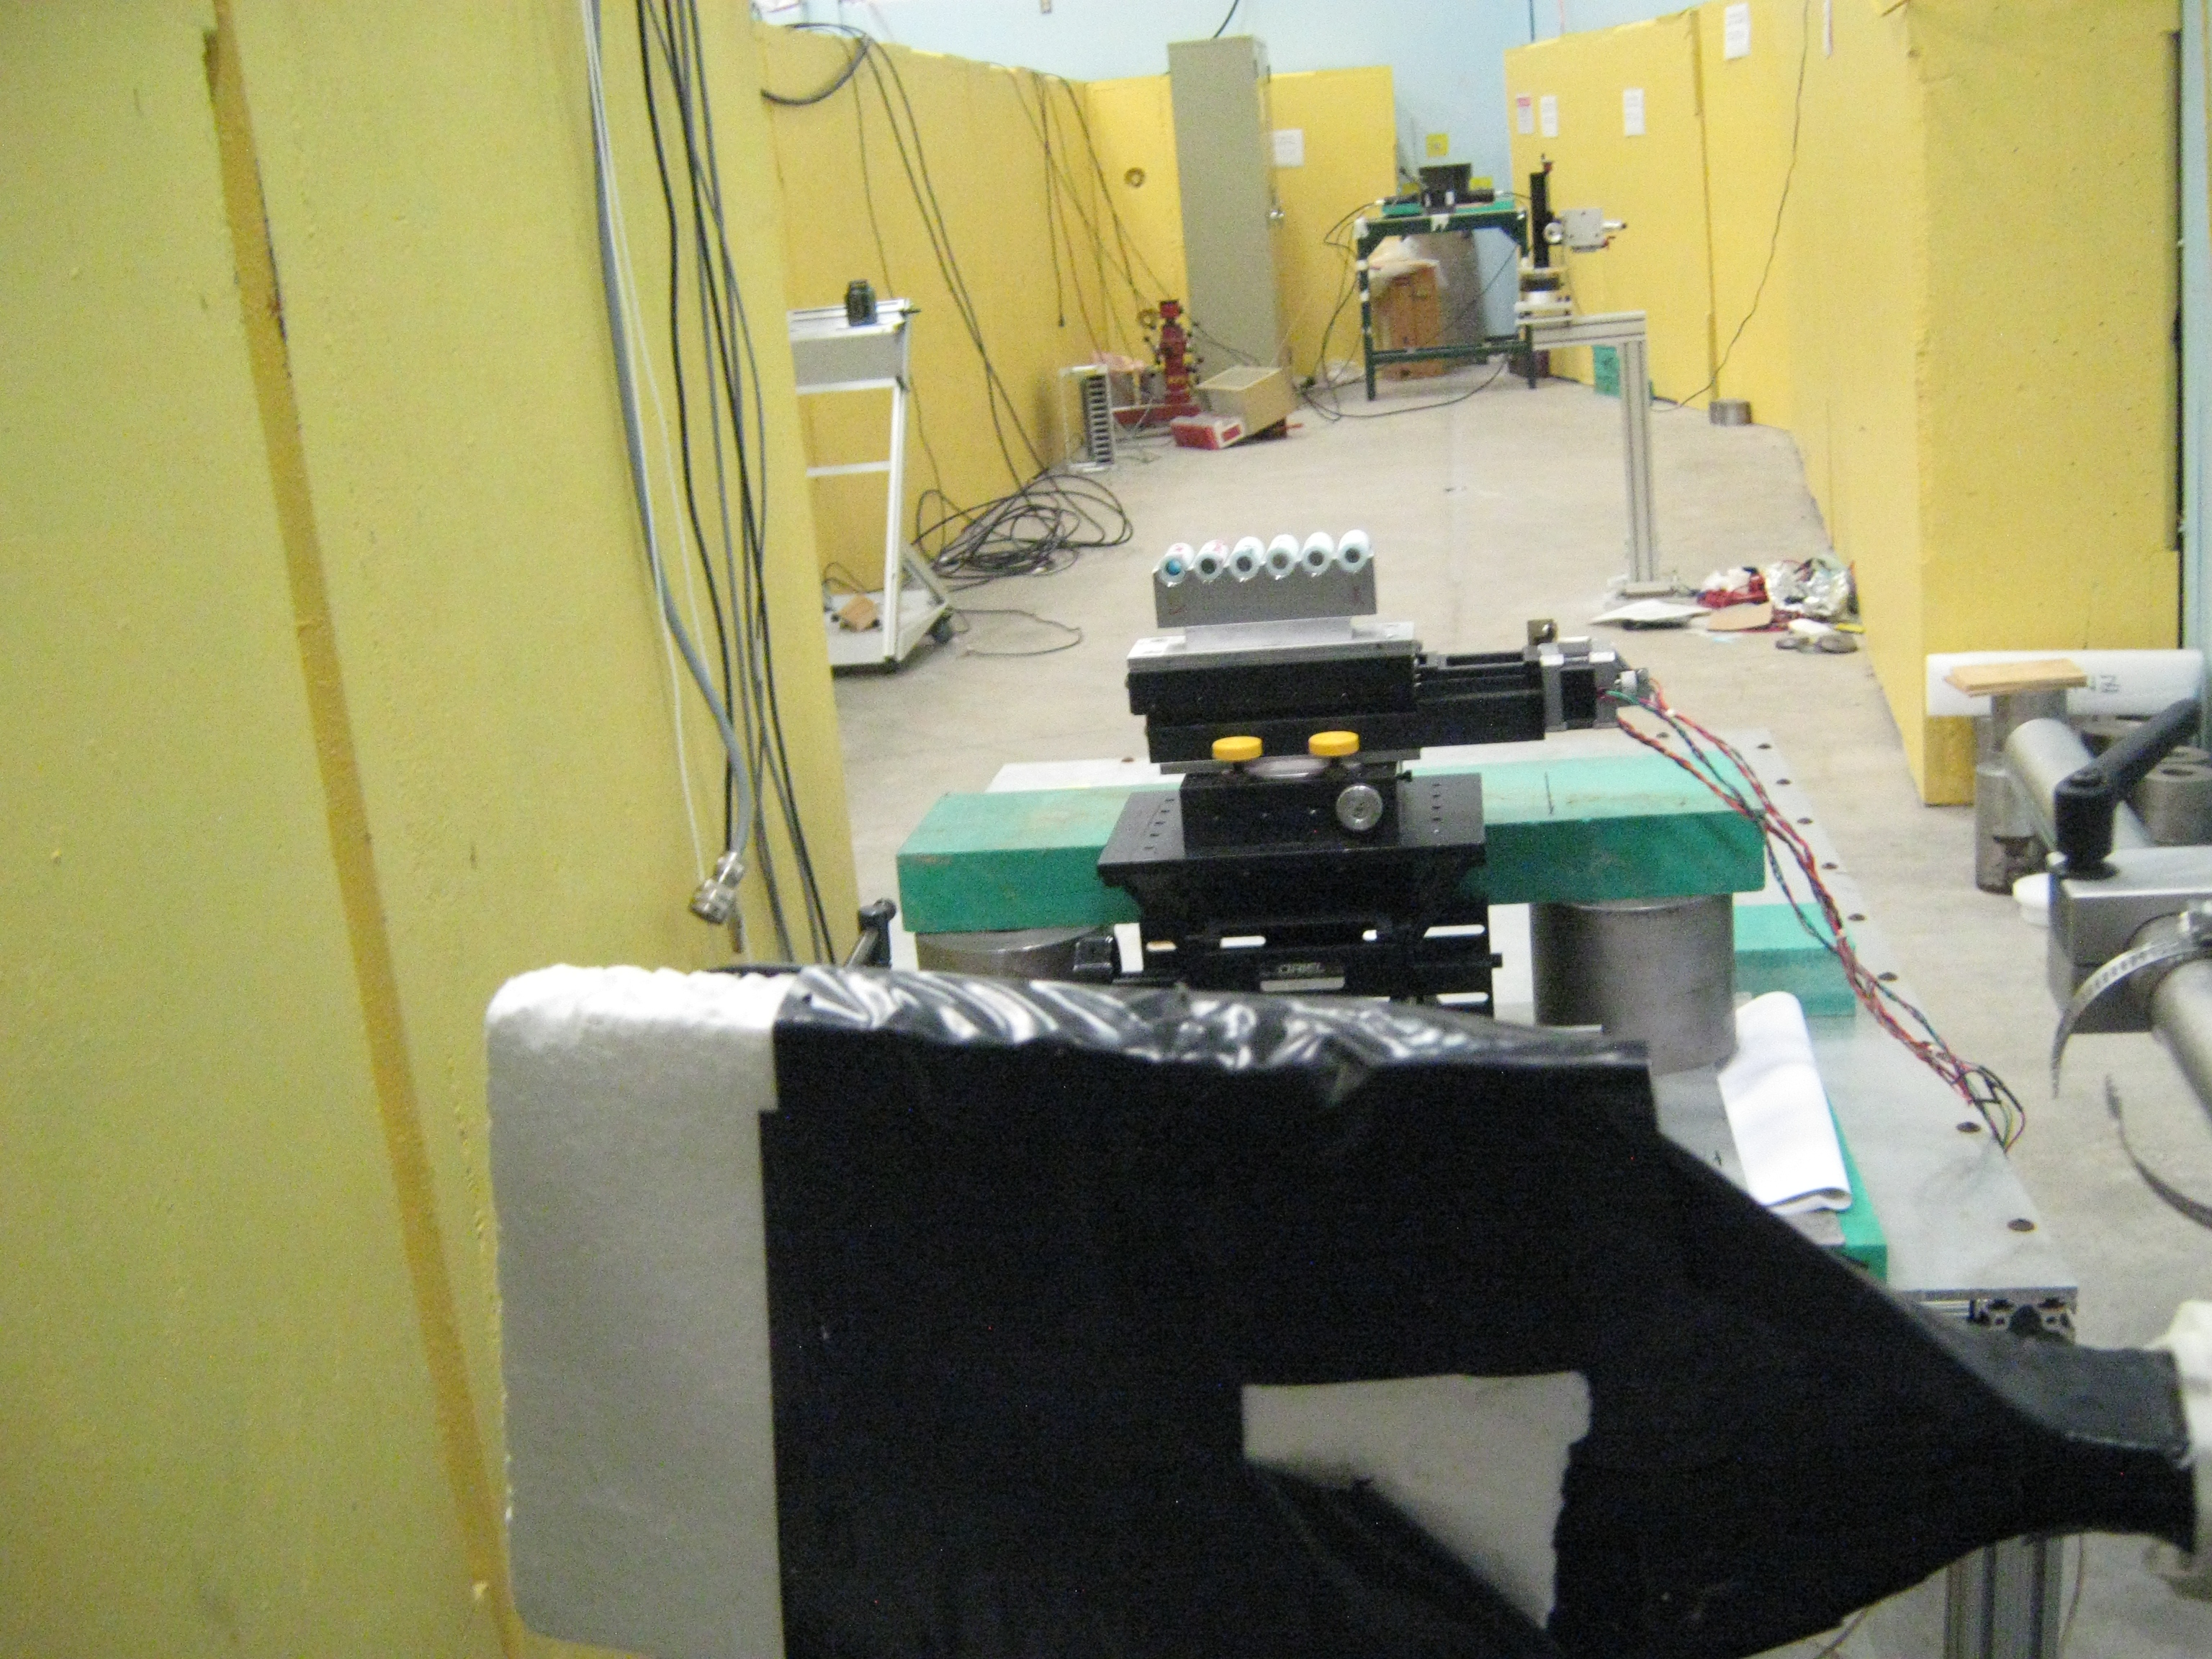
\includegraphics[width=0.9\textwidth]{figures/DownstreamFromMonitor.jpg}
    \caption[Monitor detector, sample changer, and TOF detector]
    {
        Downstream view of monitor detector, sample changer and TOF detectors
        installed in the 15R beamline.
    }
    \label{BeamlineDownstream}
\end{figure}
\begin{figure}[tb]
    \centering
    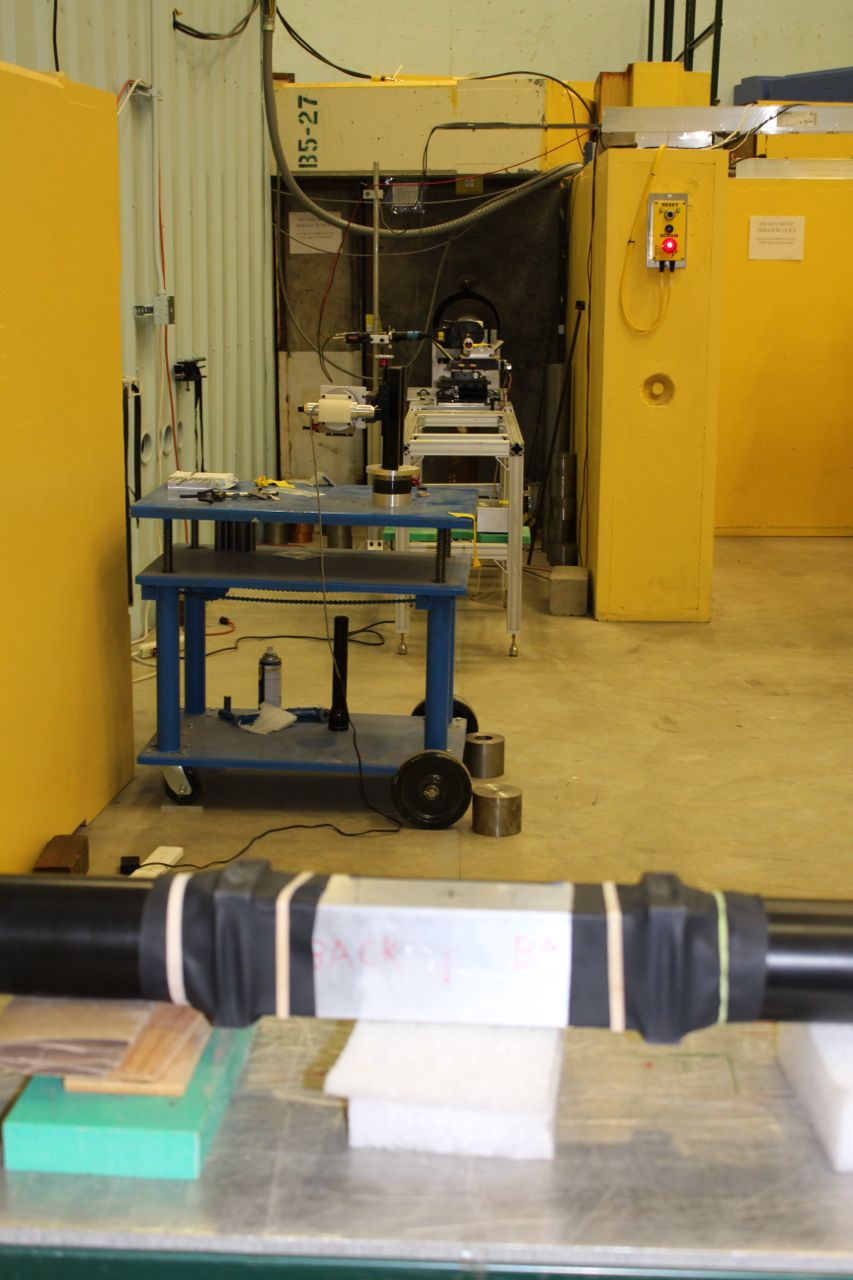
\includegraphics[height=0.8\textheight]{figures/UpstreamFromTOFDetector.jpg}
    \caption[Overview of \tot\ experimental setup in the 15R beamline]
    {Upstream view of \tot\ experimental setup in the 15R beamline. In the foreground is the
        TOF detector (the veto detector is not pictured here). In the background, the sample
    changer and monitor detector are visible. The blue cart holds the coarse-alignment laser.}
    \label{BeamlineUpstream}
\end{figure}

The particular neutron beam structure at WNR dictates the energy range
achievable for \tot\ measurements (see Fig. \ref{BeamStructure}).
\begin{figure}[tb]
    \centering
    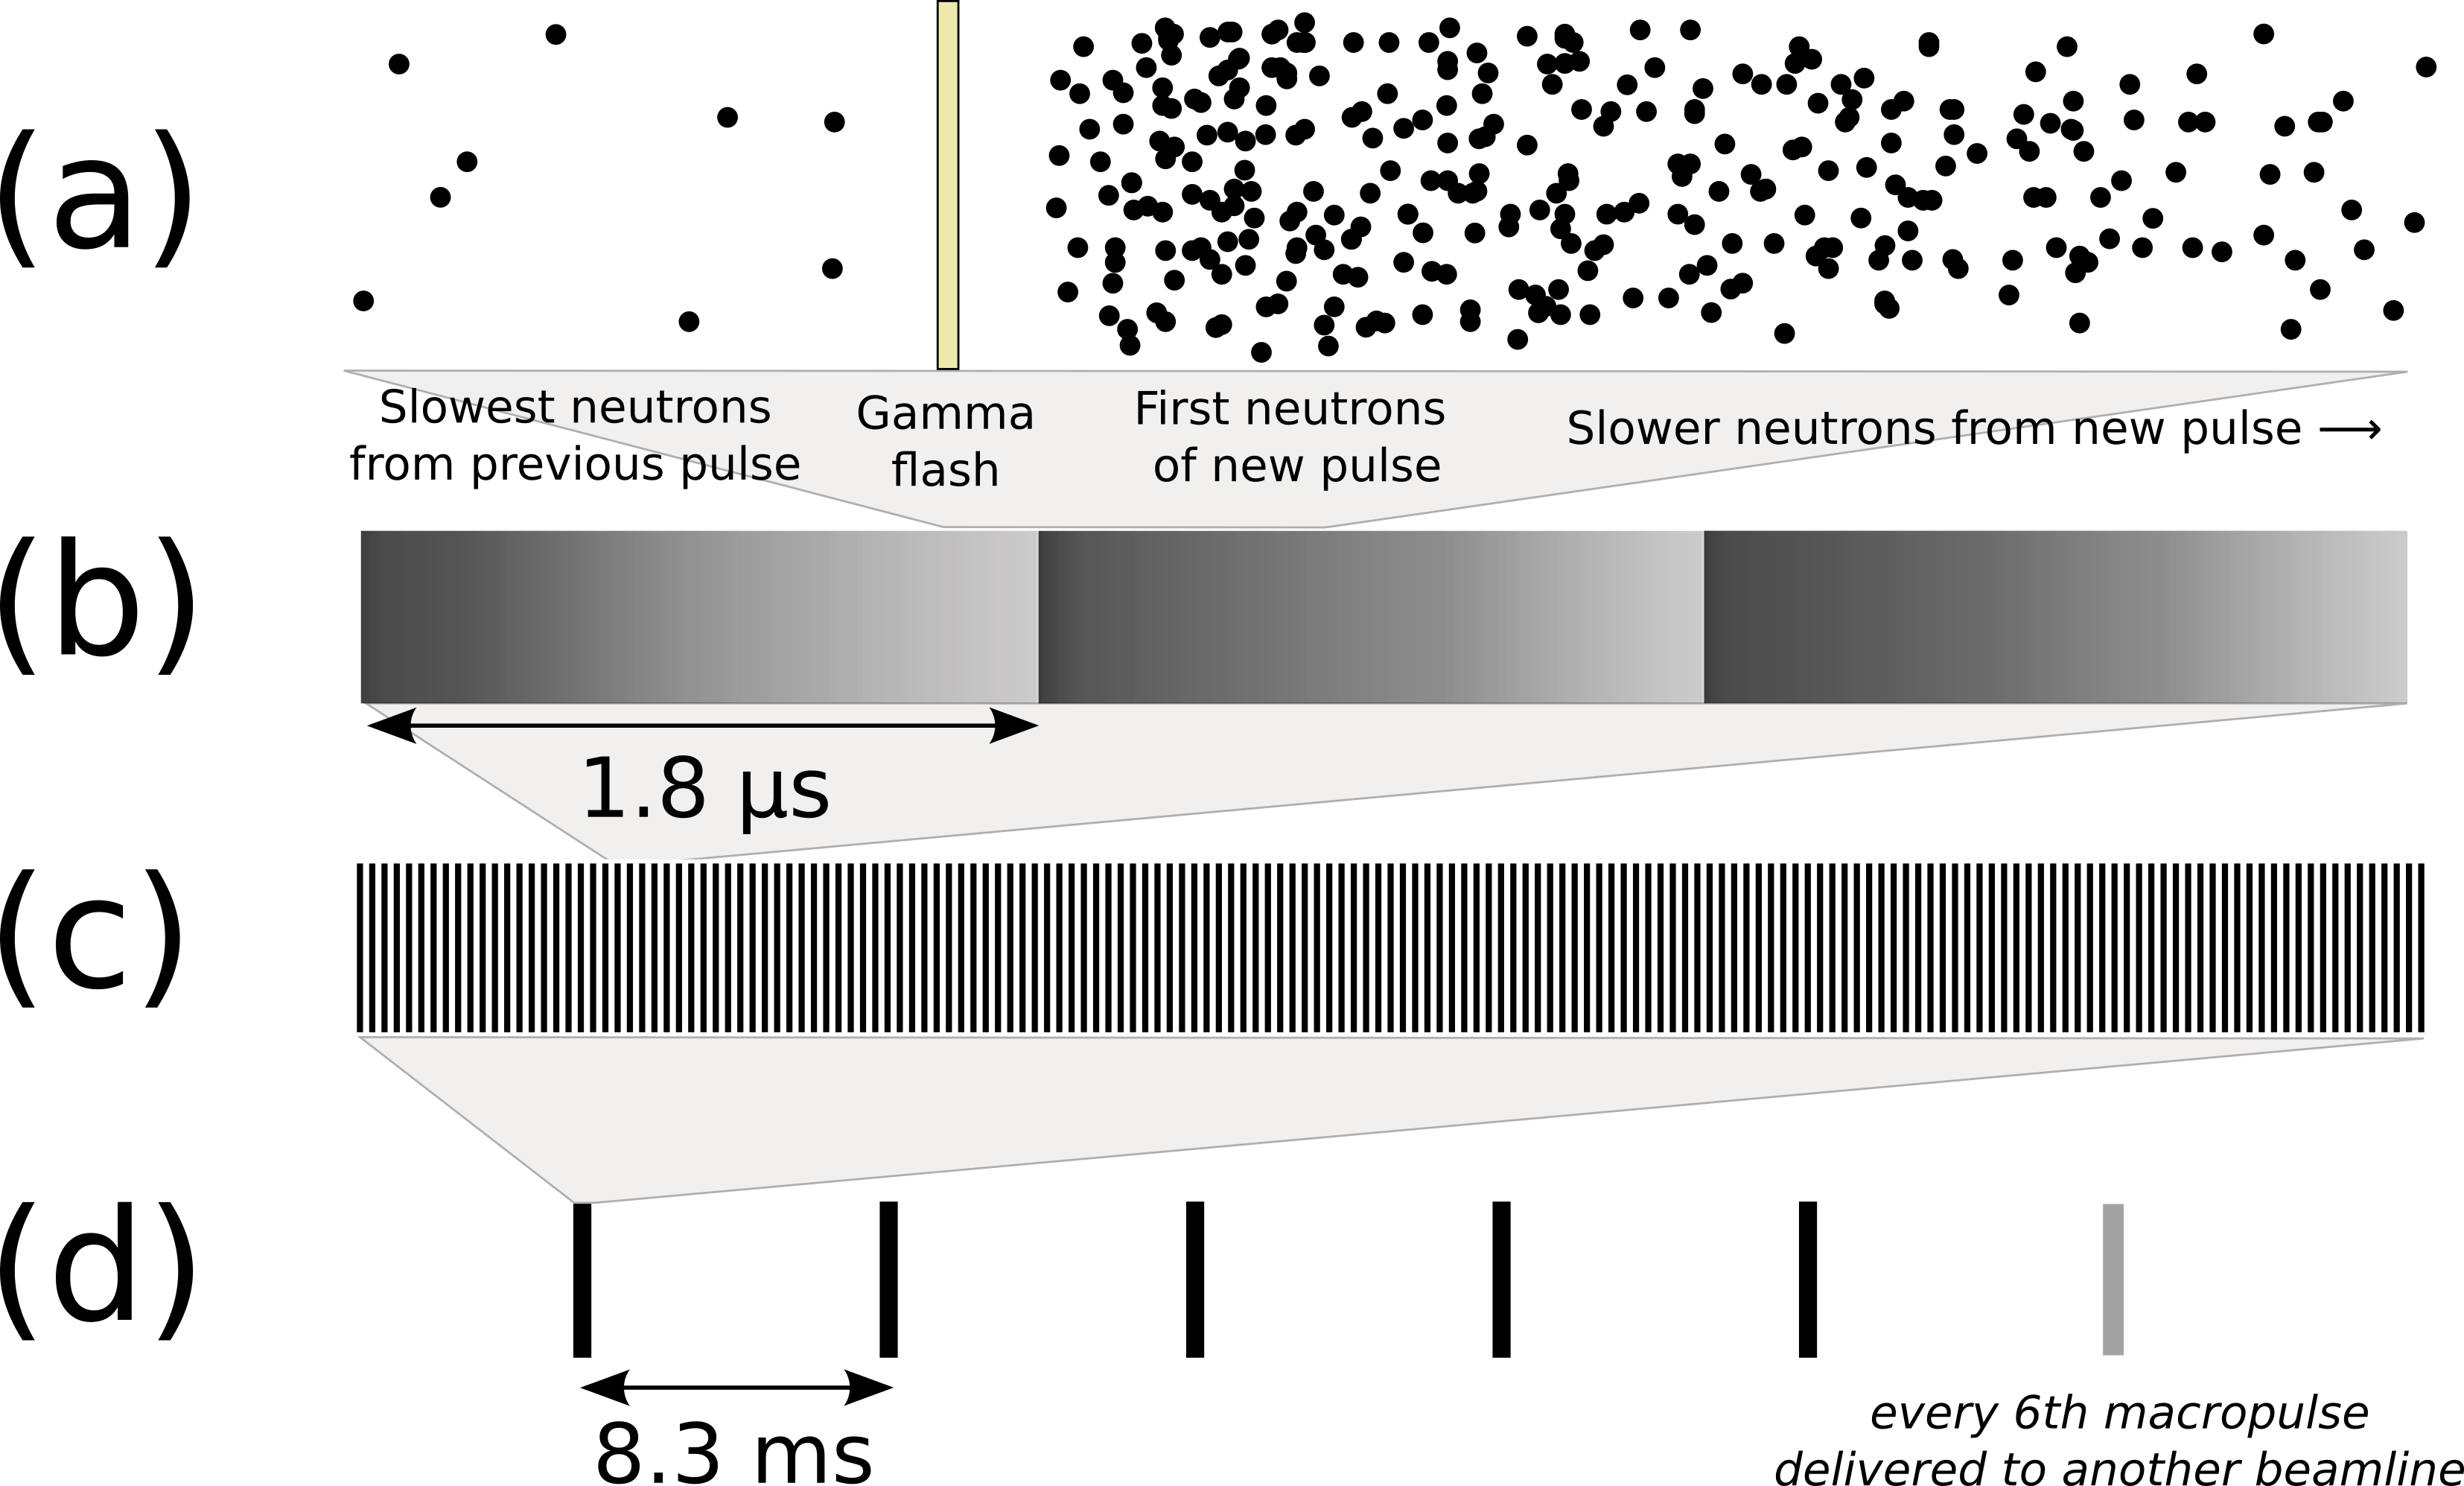
\includegraphics[width=0.9\textwidth]{figures/beamStructure.png}
    \caption[Pulsed structure of the neutron beam at the WNR facility]
    {
        Neutron beam structure at WNR facility.
        ``Macropulses'' of protons (row d) are delivered to
        WNR's tungsten Target 4, where they generate neutrons by spallation.
        Each macropulse consists of
        $\approx$350 proton ``micropulses'' (row c). Neutrons
        from each micropulse (row b) disperse in
        time as they travel along the flight path so that $\gamma$ rays and high-energy 
        neutrons catch up to low-energy ones from the previous pulse (row a).
    }
    \label{BeamStructure}
\end{figure}
Proton pulse trains, called ``macropulses'', are delivered to the tungsten target at 120 Hz.
Each macropulse consists of ~350 individual proton pulses, called
``micropulses'', spaced 1.8 \micro\second\ apart.
Each micropulse consists of a single proton packet $<$1 \nano\second\ wide when it 
arrives at the tungsten target that generates gamma rays and neutrons within a tight
temporal-spatial range. As neutrons from this micropulse travel along the beam path, 
high-energy neutrons separate in time from lower-energy neutrons so that neutron
energy can be determined by standard TOF techniques described in Chapter
\ref{TCSAnalysis} (see \cite{Moore1980} for additional details).
Because the $\gamma$ rays and high-energy neutrons from later micropulses can
overtake slower neutrons from an earlier micropulse, an important tradeoff
exists between measuring low and high-energy neutrons. The further the TOF
detector is placed from the neutron source, the higher the minimum neutron energy that can be 
unambiguously resolved. However, placing the TOF detector closer to the neutron source
increases the maximum instantaneous neutron flux at the start of each
micropulse, increasing the average per-event deadtime for the highest-energy
neutrons. A balance must be stuck between the detector thickness, the neutron
flux, the $\gamma$-ray flux, the TOF detector distance, and the rate
of data acquisition.

A programmable sample changer with six positions
was used to cycle each sample into the beam at a regular interval of 150 seconds 
per sample. Once per macropulse, an analog signal from the sample changer was recorded to 
indicate its current position. The sample configuration for each run varied, but
generally all six positions on the sample changer were used. For the solid targets,
a typical configuration was to place an empty styrofoam sample sleeve in the
first sample-changer cradle as
the ``blank'', the \cNat\ and \pbNat\ samples in the second and third
cradles, and the samples of interest (e.g., \niEight, \niNat, \niFour) in
the fourth, fifth, and sixth cradles. For water samples, an empty brass vessel
was placed in the first cradle to serve as the blank.

Due to beam divergence after collimation and the small diameter of the
samples, precise alignment of the sample changer was paramount. The sample
changer was placed on an adjustable table and roughly aligned by laser. For
precise alignment, a 2-inch aluminum cylinder with a
$\frac{1}{16}$-inch axial hole was placed
in the first position of the sample changer and a radiographic film placed
immediately posterior. The film was irradiated by the neutron beam for fifteen 
minutes and developed to show the alignment of the aluminum cylinder with the
beam profile. The position of the target changer was adjusted to improve alignment,
and the process was
iterated until alignment was satisfactory, ensuring that all neutrons
reaching the TOF detector had to pass through the in-beam sample.
Figure \ref{SampleChangerAlignment} shows a radiogram confirming alignment of all
sample changer positions within 1 mm.

\begin{figure}[tb]
    \centering
    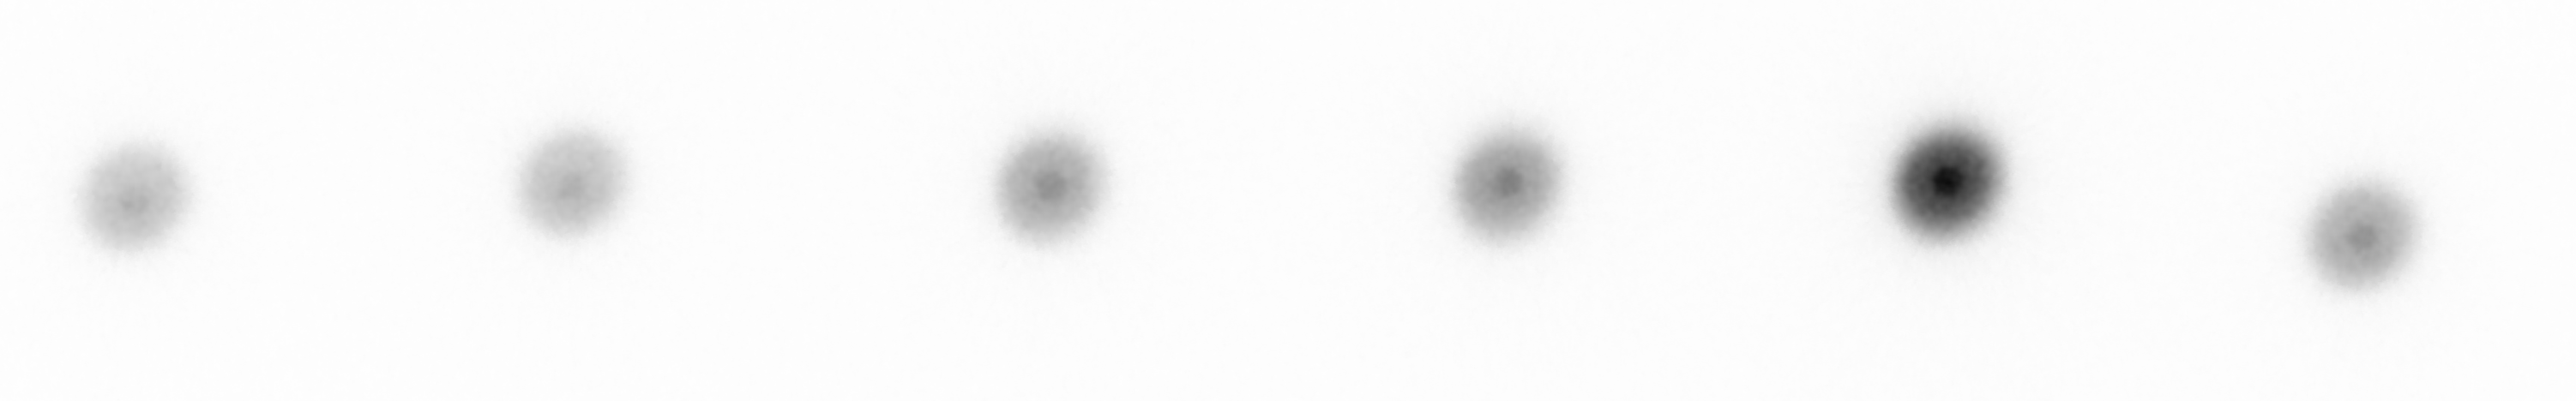
\includegraphics[width=0.8\textwidth]{figures/TargetChangerAlignment.png}
    \caption[Radiographic film showing precision alignment of the sample changer]
    {
        Radiographic film showing precision alignment of the sample changer. When the high-intensity
        central region lies in the center of the diffuse halo, alignment is achieved. All six
        positions of the sample changer were tested.
    }
    \label{SampleChangerAlignment}
\end{figure}

The beam flux of each macropulse, required to normalize absolute cross sections, was continuously
monitored by the flux monitor detector. The veto detector immediately upstream
of the TOF detector was used to reject TOF events from
charged-particle production in the samples and in air along the flight path. The
left and right PMTs of the TOF detector were gain-matched and a
0.5-ns cable delay was introduced on the right PMT signal to improve the
time-matching between the left and right signals.

\section{Data Acquisition} \label{DataAcquisition}
Signals from all detectors and the sample changer were relayed to an 8-channel, 500-MHz CAEN 
DT-5730
waveform digitizer as shown in Fig. \ref{TCSLogicDiagram}. Custom software was used to run the 
digitizer in two complementary modes, referred to as ``DPP mode'' and ``Waveform 
mode''. In DPP mode, triggers were initiated by the digitizer's onboard
peak-sensing firmware. For each trigger, several quantities were recorded: the trigger 
timestamp, two charge integrals over the detected peak with different
integration ranges (32 \nano\second\ for the short integral, 100 \nano\second\ for
the long integral),
and a 96-ns portion of the raw digitized waveform, referred to as a ``wavelet''.
The timestamp was stored as two components: a 48-bit timestamp with 2 \nano\second resolution,
and 10-bit ``fine time'' within the 2 \nano\second\ coarse time bin period.
DPP mode was used for the vast majority of the 
experiment and accounts for $\approx$99\% of the total data volume. In waveform mode, 
the digitizer performs no peak-sensing and was externally triggered. Upon 
triggering, the trigger timestamp and a very long wavelet (60 \micro\second) 
were recorded. While waveform mode data accounts for only $\approx$1\% of the total data, 
the instantaneous data rate is much higher than in DPP 
mode because hundreds of \micro\second\ of consecutive waveform samples are 
stored. Roughly once every three seconds, the digitizer was switched to 
waveform mode for one macropulse, then switched back to DPP mode as quickly as
possible (within 10-40 ms, depending on run configuration). When the buffer for
any channel filled, all buffers were read out by optical link to a flash memory
drive of the data acquisition computer, minimizing the downtime of the digitizer
due to data readout.

\begin{sidewaysfigure}[tb]
    \centering
    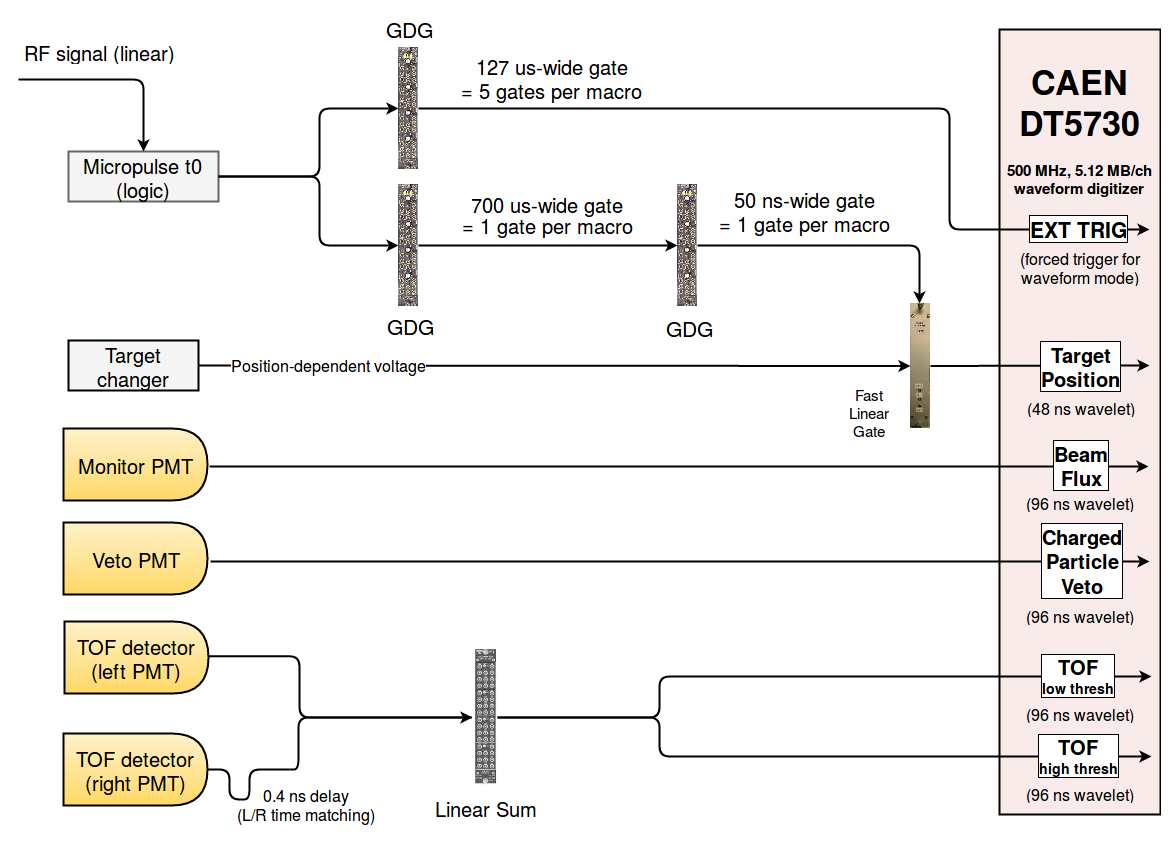
\includegraphics[width=0.9\textwidth]{figures/TCSLogicDiagram.png}
    \caption[Logic diagram for neutron \tot\ data acquisition]
    {Logic diagram for neutron \tot\ data acquisition. An explanation is provided in the text on
    page~\pageref{DataAcquisition}.}
    \label{TCSLogicDiagram}
\end{sidewaysfigure}

Because we had fast digital-signal-processing technology available, we were able
to perform event detection and processing in a fundamentally-different way
compared to analog-mediated approaches. This is worth mentioning
here as it enabled a dramatic reduction, over an order of magnitude, in the size of the
samples required compared to previous measurements at the same facility. The reasons
for our approach and tradeoffs are
described in Section \ref{DeadtimeCorrection} of Chapter \ref{TCSAnalysis}.

\afterpage{\clearpage}


\chapter{Neutron Total Cross Sections: Analysis and Results} \label{TCSAnalysis}
\section{Timing Considerations}
To assign correct neutron energies, the time resolution of the TOF
detector is critical. Several tests and corrections were applied to improve
timing resolution as much as possible.

The DT5730 provides leading-edge discrimination (\gls{LED}) and constant-fraction discrimination
(\gls{CFD}) modes for timing determination. In pre-experiment testing, we found that using the
on-board CFD calculation increased the time required to process each event by 40
ns or more, an unacceptable increase in the per-event deadtime. Thus we chose
to use the digitizer's faster LED option and to calculate precise event timing
in software, after the experiment, by analyzing the digitized waveform for each event.
Data taken from the left and right PMTs separately and gated by neutron energy 
is shown in Figs. \ref{LRCorrelation} and \ref{LRTimeDifferenceByEnergy}. 
For each energy range, the FWHM of the distribution was calculated and a hyperbolic fit was
performed, shown in Fig. \ref{DifferenceThresholdsFit}. The inherent left-right timing 
resolution, independent of neutron energy, was identified as 0.34 ns FWHM.
When folded over the actual beam energy profile (as during the experiment)
the left-right time resolution degraded to 0.52 ns.

\begin{figure}[tb]
    \centering
    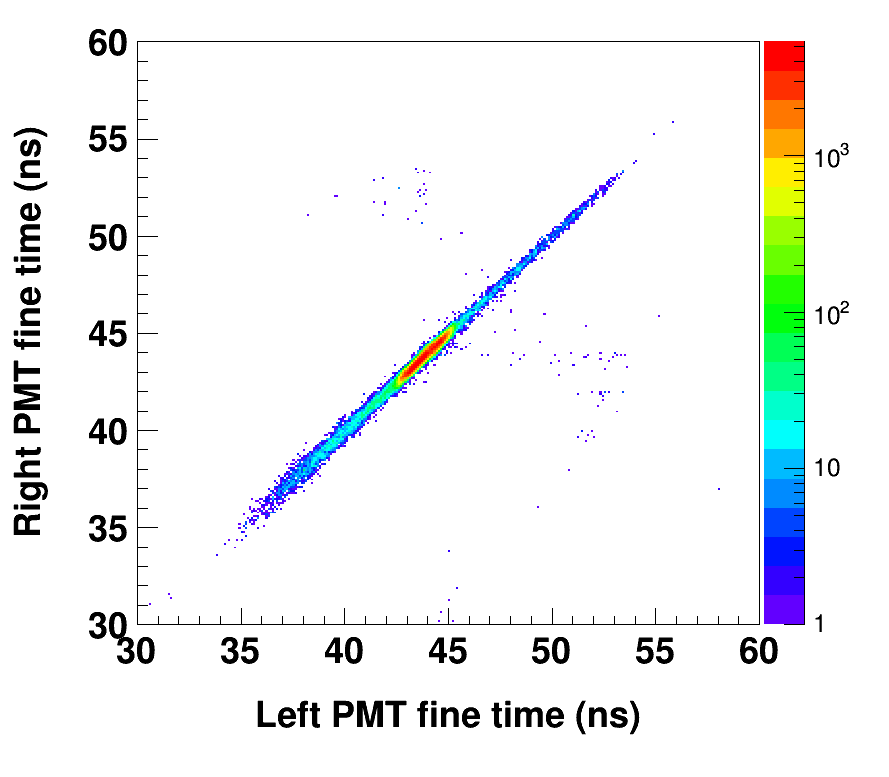
\includegraphics[width=0.8\textwidth]{figures/LRCorrelation.png}
    \caption[Event times for left and right PMTs of time-of-flight detector]
    {Fine times for left and right PMT events, taken separately, of the TOF 
        detector as recovered by our software \gls{CFD} algorithm. The times plotted are referenced
        to the start of each event waveform, which varied by several ns event-to-event.
        Thus the spread from 35-
        55 ns depends on where the digitizer initiated the waveform for each
        event and does not indicate timing resolution information.}
    \label{LRCorrelation}
\end{figure}

%\begin{figure*}
%    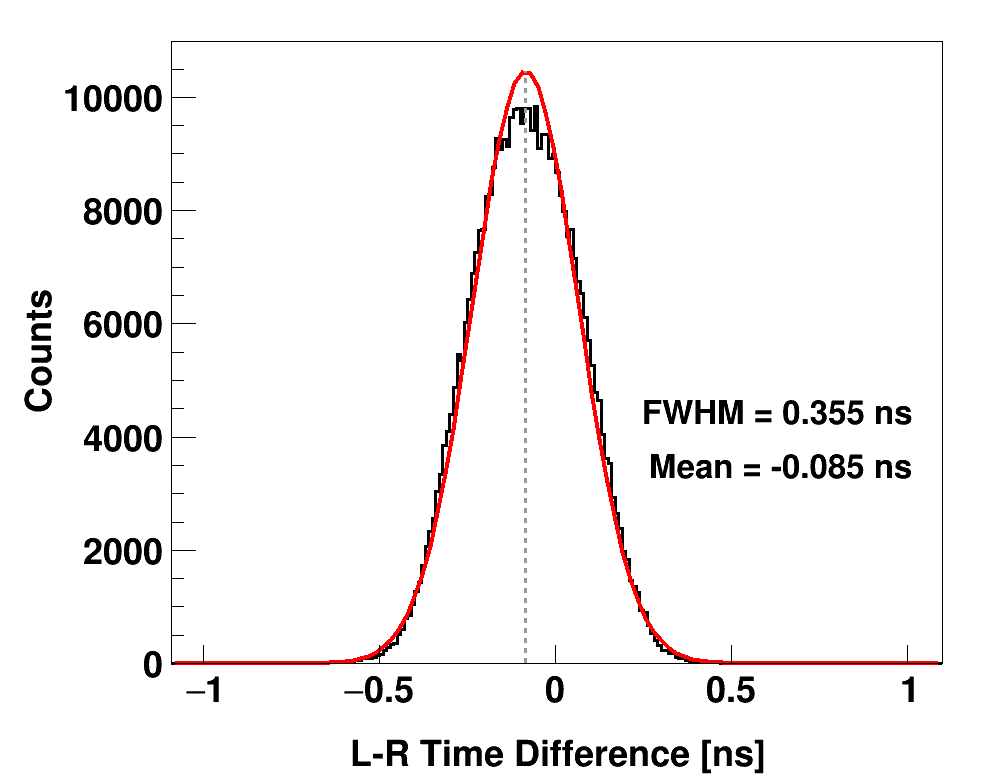
\includegraphics[scale=0.3]{figures/Difference_Linear.png}
%    \caption[Time difference between left and right PMTs of TOF detector] {
%        For all events in a diagnostic run, the time difference   
%        between the left and right PMTs of the TOF detector is plotted.
%        A Gaussian fit (in red) to these events reveals an 85-ps delay of the right PMT with 
%        respect to the left PMT and a left-right time difference FWHM of 355 ps.
%    }
%    \label{LRTimeDifferenceLinear}
%\end{figure*}

\begin{figure}[tb]
    \centering
    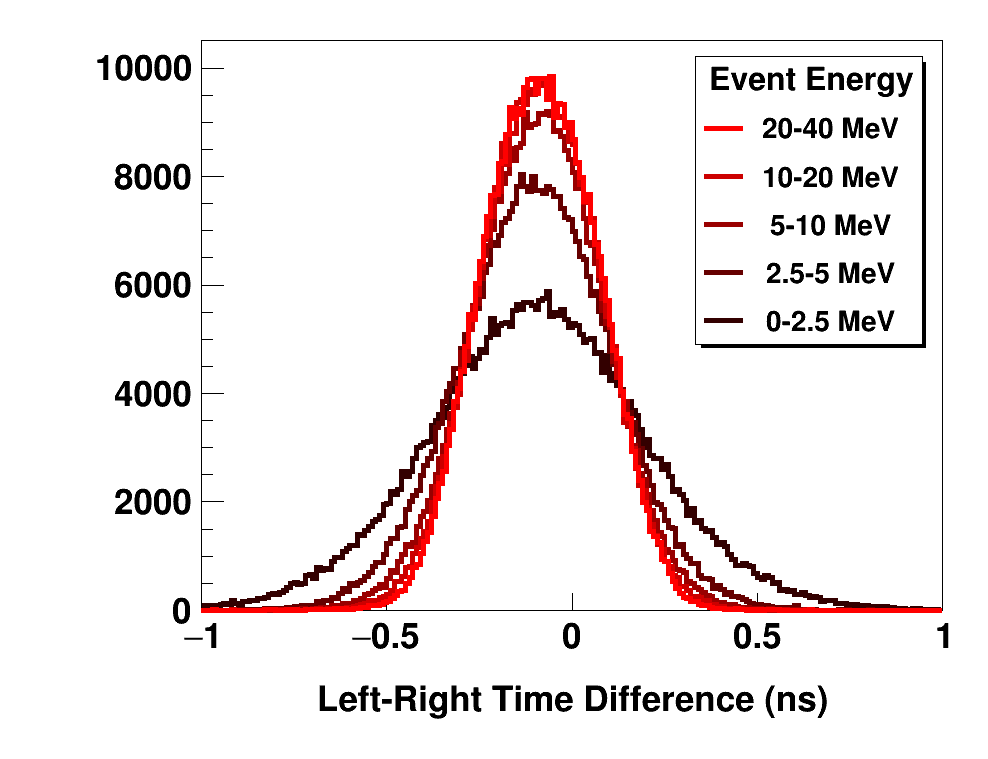
\includegraphics[width=0.8\textwidth]{figures/LRDifferenceByEnergy.png}
    \caption[Effect of energy gating on left/right PMT time difference]
    {
        Effect of energy gating on the left/right PMT time difference. Higher-energy neutrons 
        traverse also deposit more energy on average, slightly improving the
        precision of the software CFD. The same number of events were populated into each
        energy-range histogram.
    }
    \label{LRTimeDifferenceByEnergy}
\end{figure}

\begin{figure}[tb]
    \centering
    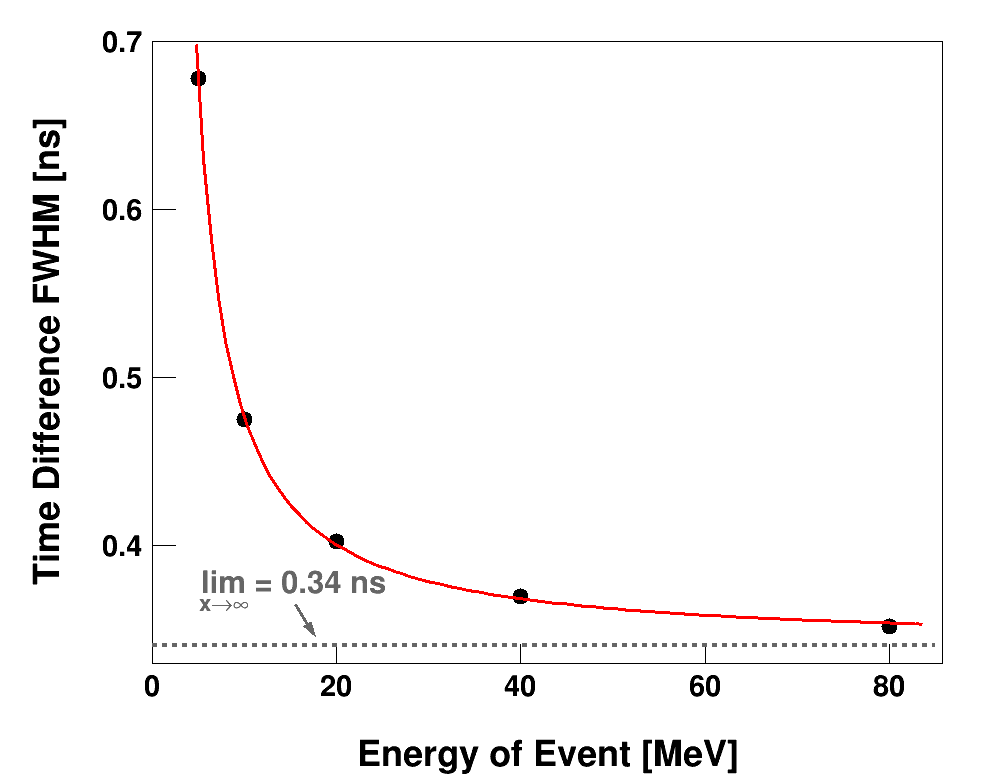
\includegraphics[width=0.8\textwidth]{figures/DifferenceThresholdsFit.png}
    \caption[Intrinsic time resolution of time-of-flight detector as a function
    of signal amplitude]
    {
        The time difference between the left and right PMTs
        of the TOF detector was calculated for all events in a diagnostic run.
        The FWHM of these time differences as a function of
        neutron energy are shown (black points) and fitted with a hyperbolic
        curve (red line). For low-energy
        events, the time resolution is poorer due to the lower signal amplitude.
        As energy increases, the FWHM time resolution asymptotically approaches 0.34
        ns (grey dashed line).
    }
    \label{DifferenceThresholdsFit}
\end{figure}

To calculate the TOF for each event, the ``starting gun'' of each
micropulse had to be precisely determined. All event times were first adjusted for cable and 
electronics delay, so that each event was assigned to the correct macropulse.
To reduce unnecessary data collection, we collected only the first \tZero, a
logic signal, of each macropulse. 
Using this time and the precisely-known micropulse frequency, we identified all $\gamma$ rays 
for a given macropulse and tabulated
the average $\gamma$-ray TOF, as shown in Fig. \ref{GammaCorrection}.
The uncertainty of our macropulse start time manifests as a spread in average gamma times-of-
flight. Were the start time exactly known for each macropulse, and the
micropulse period exactly known, the TOF for each $\gamma$ ray would be
exactly the same, ignoring the detector time resolution. Thus, the difference between the 
average calculated gamma times-of-flight (using the imprecise macropulse start
time) and the \textit{expected} TOF (given the TOF detector distance and speed of light)
can be used to improve the macropulse start time. This $\gamma$-averaging
procedure was applied to all events in each macropulse (see Fig.
\ref{TimingCorrectionStudy}). We also examined the stability of the \tZero\
period and found that its day-to-day variation had a negligible effect on the
calculated times-of-flight (see Fig. \ref{RFTimeStudy}).

After these corrections, the total TOF
resolution, taken as the FWHM of the $\gamma$-ray peak in the TOF
spectrum, ranged from 0.60-0.90 ns over the series of \tot\ measurements. This is comparable 
to the resolution from our digitizer-mediated Ca experiment from 2008 \cite{Shane2010},
which used a similar $\gamma$-averaging technique. For a 100-\mega\electronvolt\
neutron and a TOF detector distance of 27 meters, an
uncertainty of 0.80 ns translates to an energy resolution of $\approx$900 keV.
For neutrons below $\approx$20 \mega\electronvolt, the TOF time resolution worsens as the 
traversal time through the 1-inch thickness of the scintillator becomes non-negligible.
However, because the TOF of these neutrons is already several hundred ns or
longer, the relative energy resolution ($\frac{\Delta E}{E}$) is
superior at low energies. To wit, for a 5 \mega\electronvolt\ neutron with a 0.82 ns detector-traversal time and
an inherent TOF resolution of 0.80 ns, $\Delta E$ is only 13 keV. These energy uncertainties
have been propagated through the subsequent analysis.

\begin{figure}[tb]
    \centering
    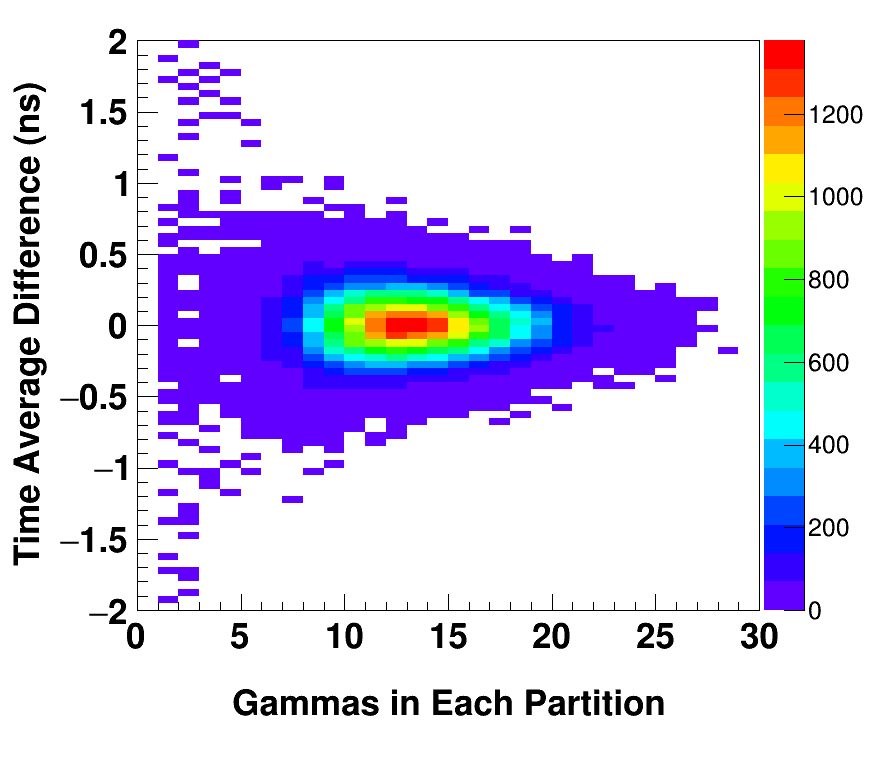
\includegraphics[width=0.8\textwidth]{figures/gammaCorrection2D.png}
    \caption[Deviation of the average $\gamma$-ray arrival time by macropulse]
    {Deviation of the average $\gamma$-ray arrival time by macropulse. }
    \label{GammaCorrection}
\end{figure}

\begin{figure}[tb]
    \centering
    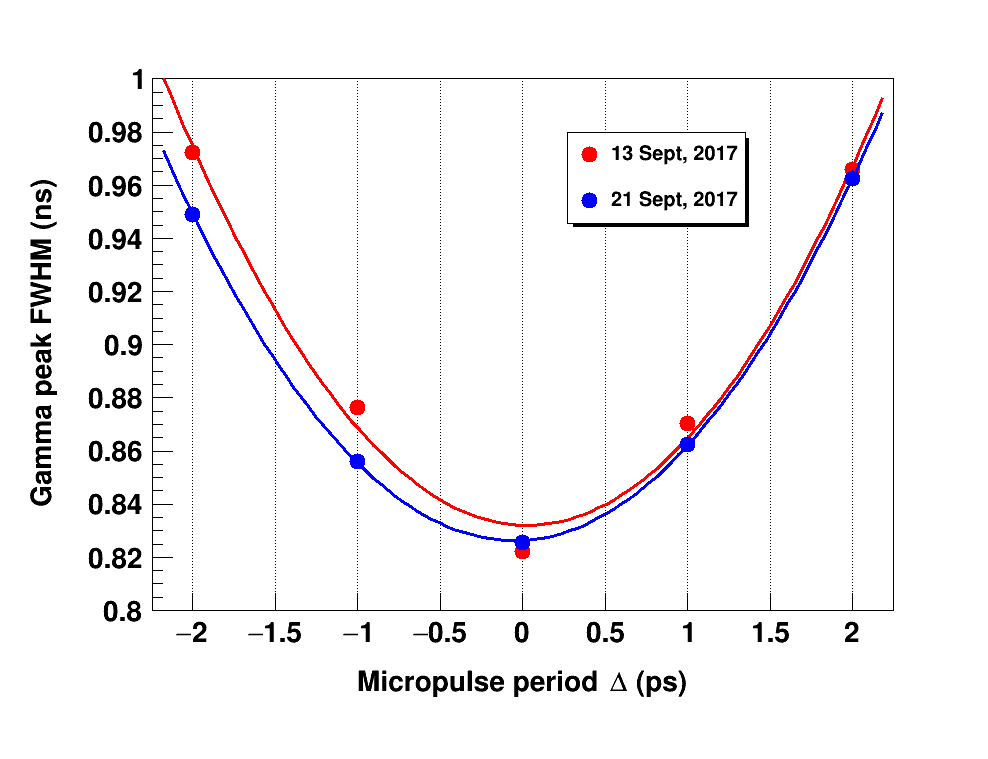
\includegraphics[width=0.8\textwidth]{figures/RFTimeStudy.png}
    \caption[Stability of the beam pick-off (\tZero) frequency during the experiment]
    {Results of a study of the micropulse frequency (\tZero) stability. The \tZero\ period used
        in the analysis was varied in 1-picosecond increments to change the
        calculated arrival TOF of events in each micropulse.
        Within each micropulse, the FWHM of
        the time uncertainty in the $\gamma$-ray flash was tabulated. The
        variation of the $\gamma$-ray flash FWHM from varying the micropulse period was
        then fitted with a quadratic curve (solid lines). The true micropulse
        frequency was taken as the minimum of this curve. This procedure was
        repeated on data from different days throughout the experimental run,
        verifying that the observed drift in the micropulse frequency is small enough to have a 
        negligible effect on the recovered times-of-flight.
    }
    \label{RFTimeStudy}
\end{figure}

\begin{figure}[tb]
    \centering
    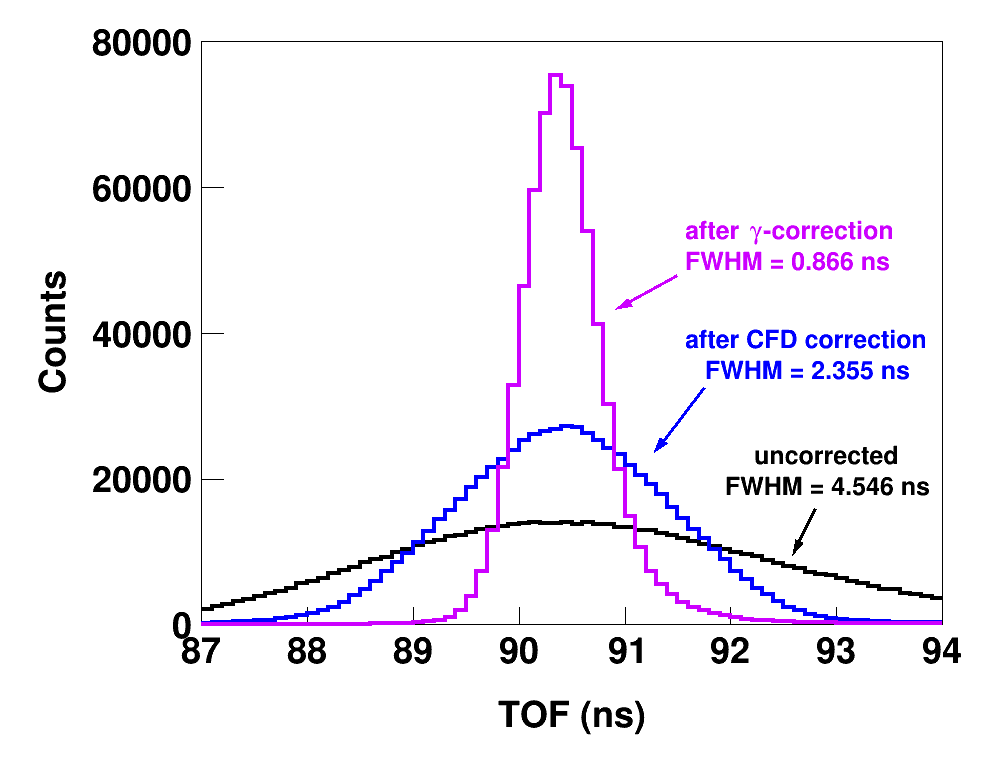
\includegraphics[width=0.8\textwidth]{figures/TimeCorrections.png}
    \caption[Improving timing precision with a software CFD and $\gamma$-ray averaging]
    {The effects of timing corrections on the $\gamma$-ray
        peak of a typical run are shown. The uncorrected spectrum is shown in black,
        the spectrum after correction with our software CFD is shown in blue,
        and the spectrum after correction with both our software CFD and
        $\gamma$-averaging is 
        shown in pink. For this run, the final $\gamma$-ray peak 
        FWHM after both corrections is 0.866 ns, comparable to the precision we
        achieved in our Ca study \cite{Shane2010}, which also employed $\gamma$-
        averaging.}
    \label{TimingCorrectionStudy}
\end{figure}

Precise determination of the TOF distance was done by comparing our measured \tot\ data
for $^{\text{nat}}$C with the precisely known resonance structure from
3-15 \mega\electronvolt\ (Fig. \ref{DistanceStudy}).
The distance was determined as 2709$\pm$1 \centi\meter\ for the
Ni and Rh run configuration and 2554 $\pm$1 \centi\meter\ for
the Sn and O run configuration. With all corrections applied, all events in the 
TOF detector channel were filtered against events in the veto detector to remove
events caused by charged-particles created along the flight path.

\begin{figure}[tb]
    \centering
    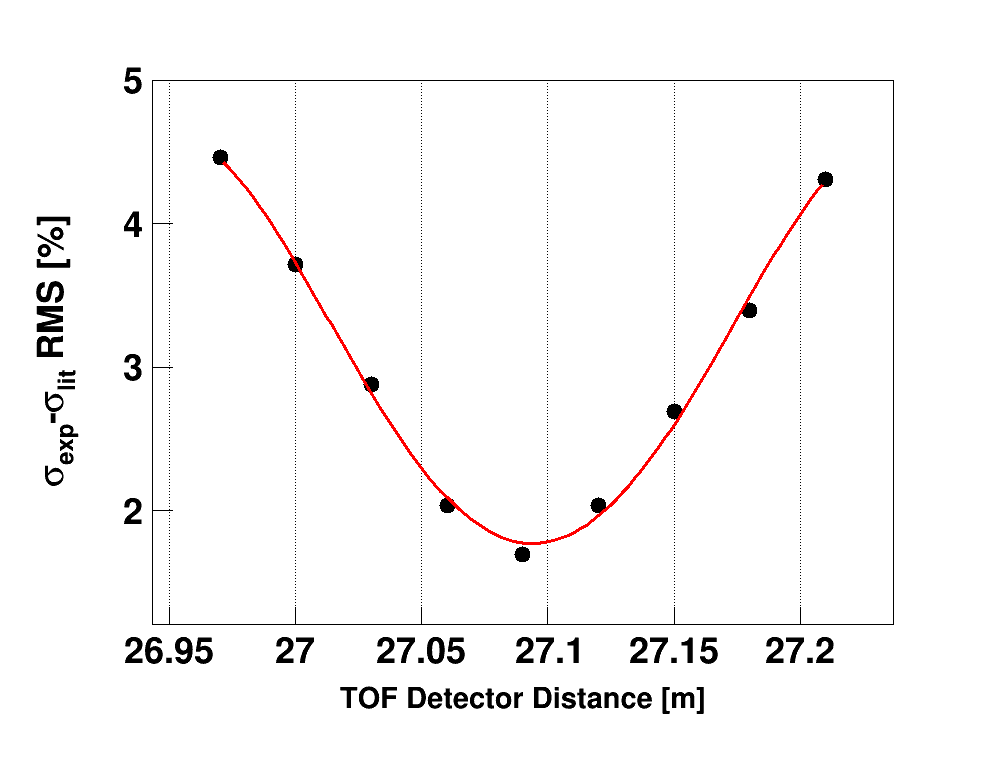
\includegraphics[width=0.8\textwidth]{figures/DistanceStudyNi.png}
    \caption[Determining the time-of-flight detector distance using \cNat\ resonances]
    {Results of a study to determine the distance between
    the neutron source and the TOF detector for the Ni/Rh running configuration
are shown. First, a plausible range of flight path distances (26.97-27.21 m) was
selected based on rough estimation during the experiment. Using each
distance in this range, the \tot\ for natural carbon was calculated in the
resonance region (3-15 \mega\electronvolt). The RMS difference between the cross section
generated using that distance and literature data from Abfalterer
\cite{Abfalterer2000, Abfalterer2001} was calculated (shown as black points in
the figure). A quartic fit to these RMS data is shown (solid line). By minimizing the
RMS difference, the flight path distance of 2709$\pm$1 cm was determined for the
Ni and Rh run configuration.}
    \label{DistanceStudy}
\end{figure}

\section{Deadtime Correction} \label{DeadtimeCorrection}
Because events are not processed instantaneously, there is a brief period
after each trigger during which the digitizer is busy processing that trigger.
The busy period following each event is referred to as the ``analytic'' or
``per-event'' deadtime and can be corrected for according to standard techniques \cite{Moore1980}.
In an ideal experiment, the instantaneous flux at all times would be
sufficiently low (and the amount of beam time available sufficiently high) that
only very rarely would another event arrive at the TOF detector while
a previous event was still being processed. In reality, given the low duty
factor of the pulsed beam, the flux during each pulse must be high to achieve sufficient
statistics over dozens or hundreds of energy bins within a few weeks of beam
time. Given the extremely small areal density of our targets, this meant a rate
of approximately one event per micropulse on average. Even with a flat
TOF spectrum, a sizable fraction of events would arrive in the shadow
of the previous event's processing period, and thus be ignored by the pulse-processing firmware.
In reality, the
problem is far worse, as the instantaneous flux is much higher during the gamma
flash and arrival of high-energy neutrons.

In \cite{Finlay1993, Abfalterer2001}, this problem was addressed by using a
``looking period'' logic. Arriving T$_{0}$ signals were used to begin a ``looking 
period'' during which neutron and $\gamma$-ray
events could be collected. At the time of the T$_{0}$ arrival, if the electronic modules
were still busy from processing a previous event (as indicated by a ``system
busy'' signal),
the looking period was aborted. During a looking period, if a single neutron or gamma
was detected, no subsequent events were allowed in the period.
This logic is diagrammed in Fig. \ref{AnalogLogic}, reproduced from
\cite{Abfalterer2001}. The fraction of T$_{0}$ signals that result in looking
periods ($\frac{T_{0,live}}{T_{0}}$) is tabulated, as is the so-called ``analytic deadtime'', i.e. 
the chance that the detector is busy for a given time \textit{within each looking period}.
TOF histograms are then scaled by these
fractions to recover the true number of events per unit flux. This approach is useful if the
analytic deadtime is commensurate with the micropulse period, as it means that
only one event can be detected per micropulse anyway. For this approach to be successful, the
analytic deadtime must be very precisely known, as corrections can soar to over 100\%
if the beam flux is high.

\begin{figure}[tb]
    \centering
    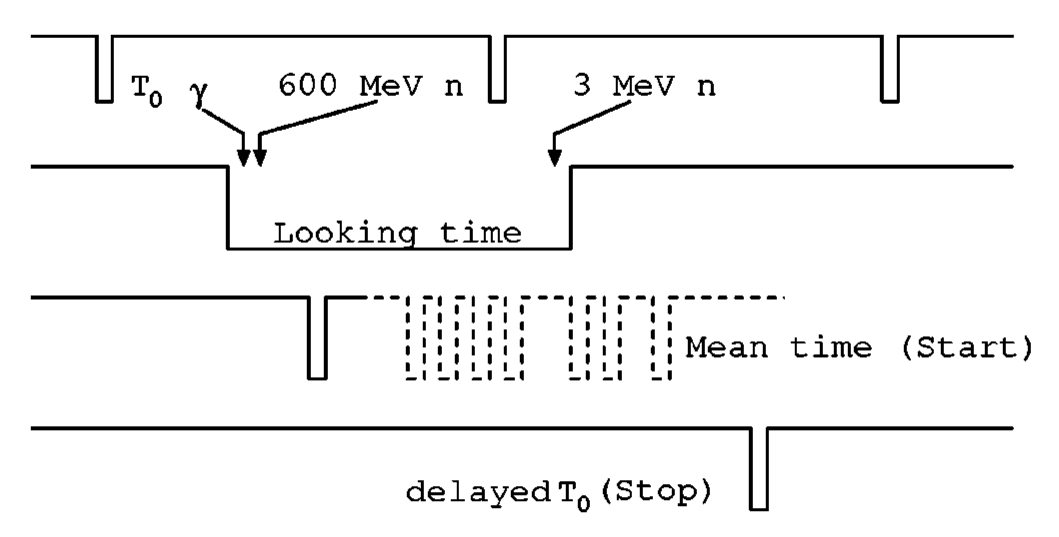
\includegraphics[width=0.8\textwidth]{figures/AnalogLogic.png}
    \caption[``Looking period'' logic from previous neutron \tot\ measurements at LANSCE]
    {
        ``Looking period'' logic used by previous neutron \tot\ measurements at LANSCE
        \cite{Abfalterer2001}. Per the original caption: proton beam bursts arriving at
        evenly-spaced 1.8-$\mu$s time intervals define a time frame 1.4-1.6 $\mu$s long. For each
        time frame, a delayed copy of the \tZero\ defining it was used as a stop signal on the TDC
    clocks. In contrast, the event processing logic of our experiment dispensed with looking 
    periods to maximize the number of neutrons detected.}
    \label{AnalogLogic}
\end{figure}

Due to the extremely low areal density of our samples,
we could not afford to discard any neutron events and still acquire sufficient statistics. 
Thanks to the dramatically-reduced analytic deadtime of the digitizer algorithm,
we could use a more straightforward deadtime correction logic and minimize the
number of lost events. Assuming negligible variation in beam flux between micropulses
(an assumption investigated below), the fraction of time $F[i]$ that the digitizer is dead 
for a given time bin $i$ can be calculated:
\begin{equation}
    F_{i} = \sum^{N-1}_{j=0} R_{(i-j)\text{ mod N}}\times P_{j}
\end{equation}

\noindent
where $N$ is the number of time bins in the micropulse, $R_{x}$ is the rate of
detected events per micropulse in bin $x$, and $P_{j}$ is the probability that the
digitizer is still busy from a trigger $j$ bins ago. Moore \cite{Moore1980} also provides
a more general 
formula to calculate the appropriate deadtime correction in cases where the variation in beam 
flux is significant. However, an examination of our flux-per-micropulse data 
showed almost no variance in the flux per micropulse, except during the first 10\%
of each macropulse when flux was ``ramping up''. In our final analysis, we have discarded the 
first 40 micropulses of each macropulse and used the simpler Eq. \ref{DeadtimeEquation} to 
calculate the deadtime fraction.

To model $P_{j}$, we
employed a logistic function and fitted it to the observed spectrum for time
differences between consecutive events (see Fig.  \ref{TimeDifferenceBetweenEvents}).
For a given bin $i$, the fraction of time that the 
digitizer is dead, $F_{i}$, is in essence a discrete convolution of the
\textit{measured} TOF spectrum with $P_{j}$. Note that except for the first and
last micropulses in a macropulse, micropulses are consecutive and thus deadtime effects can
``wrap around'' from the end of one micropulse to the next. For these wrap-around
contributions (that is, $j>i$), the (mod N) term ensures that the bin referred
to by $(i-j)$ is non-negative and has physical meaning as a time bin from the previous 
micropulse.

By optimizing trigger processing in digitizer firmware,
we were able to reduce the per-event deadtime to between 160-230 ns,
depending on the digitizer configuration.
For a 230 ns per-event deadtime, the dead-probability
$F_{i}$ of our time bins is given in Fig.
\ref{ExampleDeadtimeSpectrum}, showing that the probability-dead never exceeds
25\%, much smaller than the 50-80\% typical in the approach described above
\cite{Finlay1993, Abfalterer2001}.
Once the fraction dead was identified for each time bin, the total number of
events detected in that bin, $N_{d}[i]$, was corrected to the \textit{true}
number of events in that bin $N_{t}[i]$ that would have been detected in the
absence of a per-event deadtime:
\begin{equation} \label{DeadtimeEquation}
    N_{t}[i] = -ln\left[1-\frac{\frac{N_{d}[i]}{M}}{(1-F_{i})}\right]\times M
\end{equation}

\noindent
where M is the total number of micropulse periods. The difference between
uncorrected and analytic-deadtime-corrected TOF spectra is shown in Fig.
\ref{CorrectionEffectOnTOF}. At large TOFs (low energies) the correction is as low as a
few percent, but at small TOFs (high energies) when the digitizer is still dead
from the $\gamma$-ray flash and high-energy neutrons, the correction is significant
($\approx$20\% for our Ni/Rh runs, and $\approx$40\% for our Sn/O runs). Again, these 
corrections are themselves far lower than the correction required
when using the previous approaches \cite{Finlay1993, Abfalterer2001}, which
could be over 100\% for the lowest-energy neutrons, depending on beam flux. It is
important to keep in mind that in these experiments the probability that the
data acquisition electronics are busy is not a fixed number but a
function of the neutron energy.

\begin{figure}[tb]
    \centering
    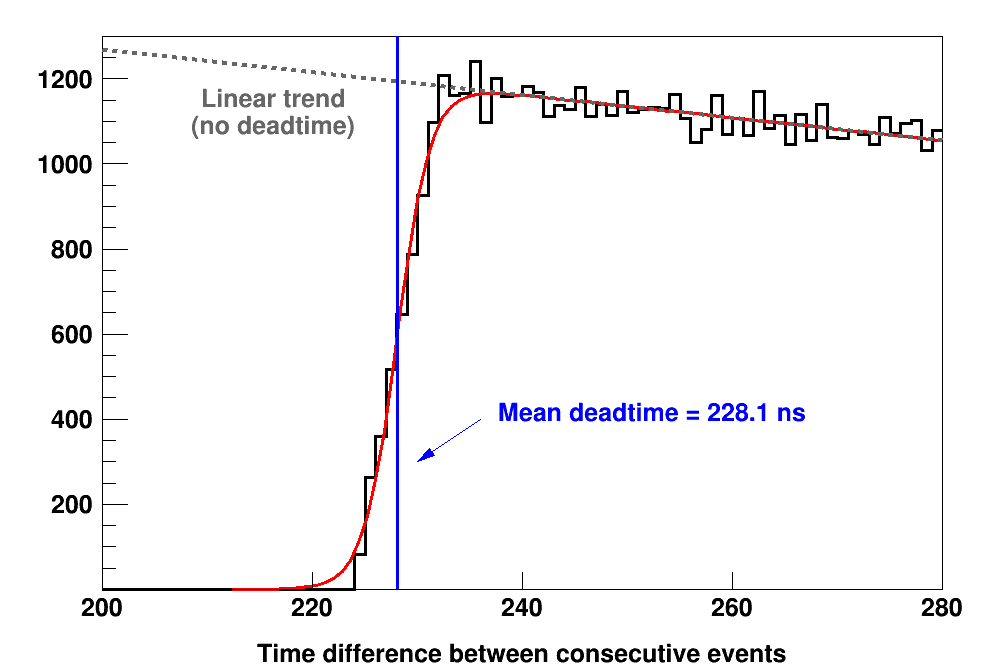
\includegraphics[width=0.8\textwidth]{figures/TimeDifferenceBetweenEvents.png}
    \caption[The time difference between consecutive events in the time-of-flight detector]
    {The time difference between adjacent TOF-detector
    events for a single run is plotted (black histogram). Below a certain
minimum time difference (the ``deadtime''), no events are recorded. A logistic
fit (red) models the detector's deadtime response and is used to generate a
deadtime correction. The underlying linearly-decreasing count rate (gray dashed
line) in incorporated into the logistic model. From the fit, a mean deadtime of
228.1 \nano\second\ was extracted for the Sn and O run configuration (a similar
procedure was used to recover a deadtime of 159.7 \nano\second\ for the Ni and Rh
run configuration).}
    \label{TimeDifferenceBetweenEvents}
\end{figure}

\begin{figure}[tb]
    \centering
    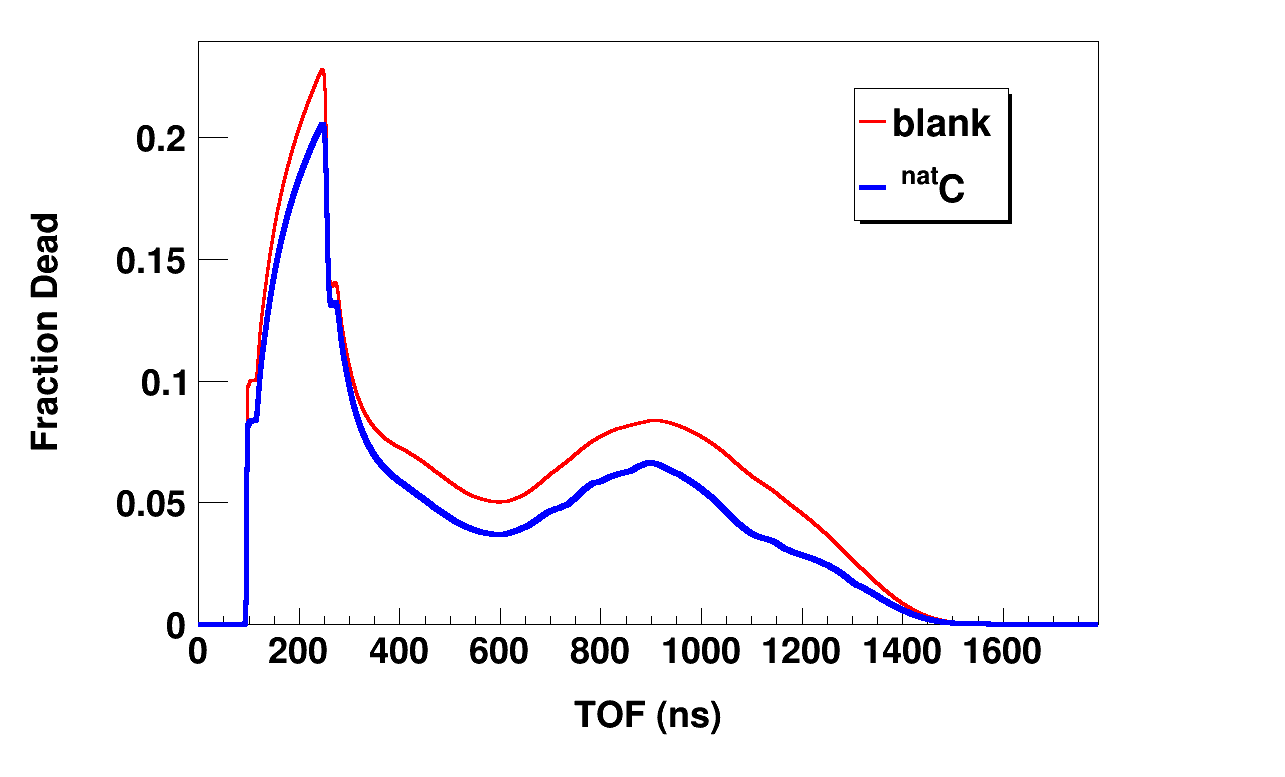
\includegraphics[width=0.8\textwidth]{figures/exampleDeadtimeSpectrum.png}
    \caption[Digitizer busy probability as a function of time within micropulse]
    {
        Using TOF data from a typical run, the fraction of time that a given 
        TOF bin is ``dead'' is shown for the blank sample (red line) and the 
        \cNat\ sample (blue line). The sharp rise at 90 \nano\second\ is the response to the
        $\gamma$-ray flash, the gradual increase from 90-245 \nano\second\ is the response to
        the arrival of high-energy neutrons, and the sharp fall at 245
        \nano\second\ is the elapse of the $\gamma$-ray ``shadow''.
        Only high-energy neutrons have a probability-dead exceeding 10\%.
    }
    \label{ExampleDeadtimeSpectrum}
\end{figure}

\begin{figure}[tb]
    \centering
    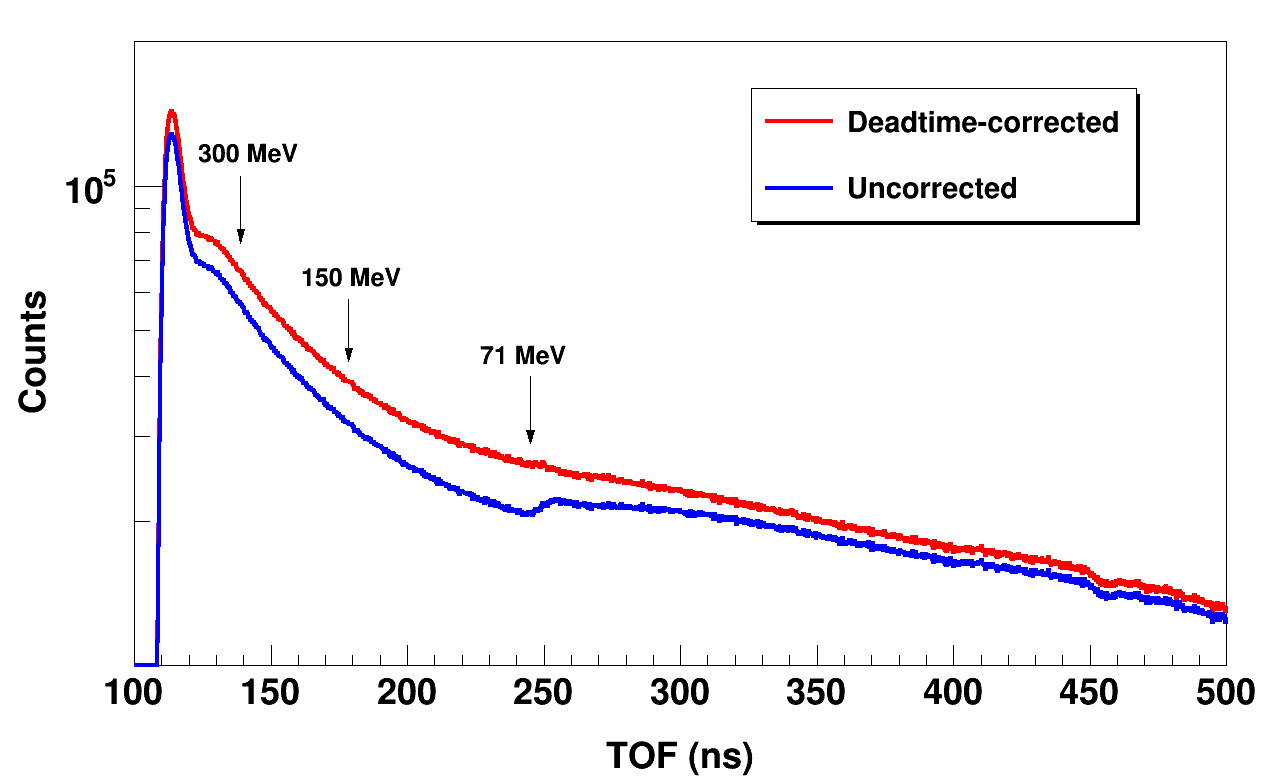
\includegraphics[width=0.8\textwidth]{figures/CorrectionEffectOnTOF.png}
    \caption[The effect of deadtime correction on a typical time-of-flight spectrum]
    {
        A typical TOF spectrum from the Ni/Rh
        run configuration is shown, before (in blue) and after (in red) analytic
        deadtime correction. Relevant neutron energies are indicated above the spectra.
        For this digitizer configuration, the mean deadtime was 155
        \nano\second\ (see Fig.
        \ref{TimeDifferenceBetweenEvents} for details on mean deadtime determination).
        Note that at 245 \nano\second, there is an
        obvious defect in the uncorrected spectrum that is repaired in the corrected
        spectrum. The defect
        corresponds to the elapse of the 155-\nano\second-long deadtime
        ``shadow'' from the $\gamma$-ray flash, which arrived at 90
        \nano\second\ (not shown).
    }
    \label{CorrectionEffectOnTOF}
\end{figure}

During analysis, it was noted that occasionally (1 in 400 macropulses), one or two 
adjacent macropulses would have an abnormally small number of flux monitor events or 
TOF events. The frequency of these ``data dropouts'' was similar to the rate of
switching between DPP and waveform modes and we suspect it is related to edge
case behavior right before or after a mode switch. To mitigate this issue,
any macropulse that had less than 50\% of the average event rate in either the
flux monitor or TOF detector channel was ignored.

After applying these corrections, the veto and integrated charge gates are applied to 
all events and surviving events are populated into TOF spectra (see Fig.
\ref{ExampleTOFSpectrum}). From these spectra, room background was subtracted
(responsible for 0.1\% to 1\% of event rate, depending on energy)
and events were mapped to the energy domain.

\begin{figure}[tb]
    \centering
    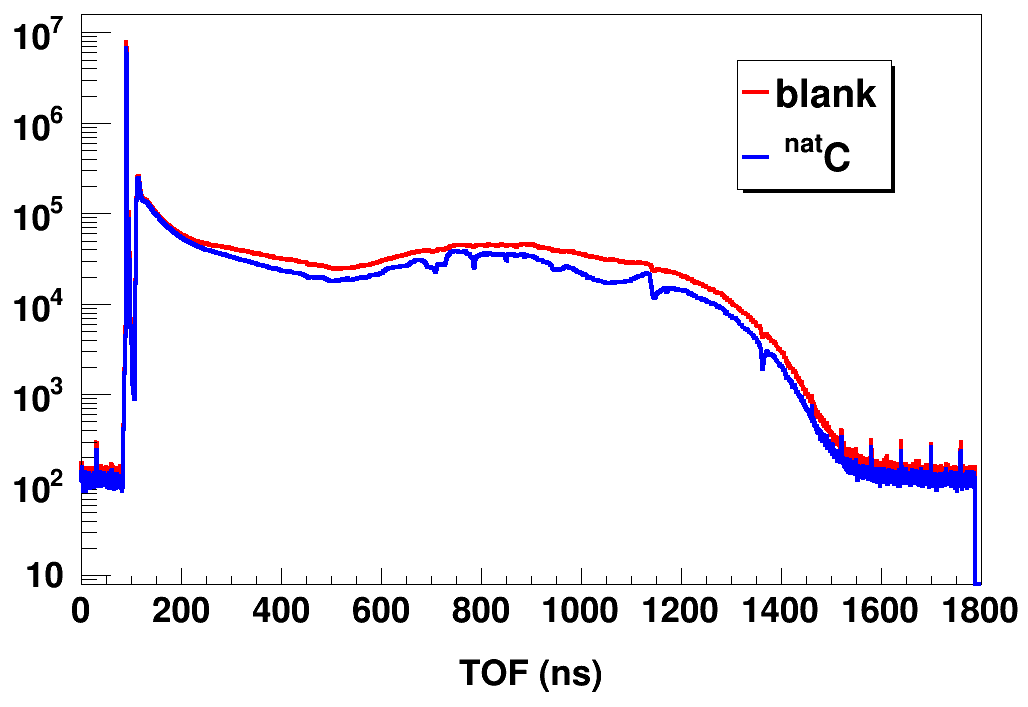
\includegraphics[width=0.8\textwidth]{figures/exampleTOFSpectrum.png}
    \caption[Typical time-of-flight spectrum after timing and deadtime corrections]
    {
        Typical TOF spectra after analytic deadtime correction and
        veto and integrated charge gating. A spectrum from the blank sample is shown in
        red and a spectrum for the $^{\text{nat}}$C sample is shown in blue, both from the Ni/Rh 
        experiment configuration.
        The $\gamma$-ray peak presents as a sharp spike at 90 ns, followed by
        the highest-energy neutrons at 130 ns. The small spikes spaced 60 ns
        apart (visible before 90 ns and after 1500
        ns) are $\gamma$-ray peaks from a low-level, continuous ``drip'' 
        of protons onto the tungsten target caused by mistuning of the proton 
        buncher; their effect on the calculated cross sections is negligible. Low-energy carbon
        resonances are visible above 600 ns.
    }
    \label{ExampleTOFSpectrum}
\end{figure}

It is worth mentioning two additional systematic differences between our configuration and
those of previous LANSCE measurements \cite{Shane2010, Finlay1993, Abfalterer2001}, namely the
flight path length and sample diameters. Flight path lengths of 37.70 meters, 38.14 meters, and 45
meters were used in \cite{Finlay1993}, \cite{Abfalterer2001}, and \cite{Shane2010} respectively, 
much longer than the 25-27 meters position of our TOF detector.
Had these lengths been available for our experiment,
it would have reduced the high-energy instantaneous neutron flux by 
$\frac{1}{3}$, potentially affecting our results for the highest-energy neutrons. Future
experimental work at the 90 meter flight path station at LANSCE would be ideal: the
instantaneous neutron flux would be reduced by more than half compared to our experiment
and neutrons as low as 10 \mega\electronvolt\ could still be unambiguously identified before micropulse wraparound.
The other major difference, the sample diameters, affects the diameter of the collimation used.
Diameters of  2.2-2.9 cm, 2.3-3.8 cm, and 1.3 cm were used for \cite{Shane2010},
\cite{Finlay1993}, and \cite{Abfalterer2001}, respectively, much larger than the 0.8 cm diameter of
our samples. As sample (and thus collimator) size decreases, the cross-sectional area of the
collimation pipe decreases compared to its circumference. At some point,
neutrons scattering at very
small angles on the interior of the collimation could become significant compared to the number of
neutrons passing through the collimation freely, distorting results.
While we see no evidence of this phenomenon affecting
our results, a collimation-scattering simulation may be warranted for
experiments with even smaller sample diameters.

\section{Cross Section Calculation}
The fundamental quantity of interest, \tot, is related to the flux
loss through a sample by:
\begin{equation}
I_{t} = I_{0}e^{-{\ell\rho\sigma_{tot}}}
\end{equation}

\noindent
or, equivalently,
\begin{equation}
    \tot = -\frac{1}{\ell\rho}ln\left(\frac{I_{t}}{I_{0}}\right)
\end{equation}

\noindent
where $I_{0}$ is the neutron flux entering the sample, $I_{t}$ is the neutron
flux transmitted through the sample without interaction, $\rho$ is the number
density of nuclei in the sample, and $\ell$ is the sample length. For thin
or low-density samples, flux attenuation through the sample will be small
(e.g., 13\% for our Ni samples at 100 \mega\electronvolt) and a large number
of counts will be required to determine the cross section to high
precision.

From these energy spectra, the raw cross sections were calculated, bin-wise, as follows:
\begin{equation} \label{CSCalculation}
    \tot = -\frac{1}{\ell\rho_{n}}
    \ln \left(\frac{I_{0}}{I_{s}}\times\frac{M_{s}}{M_{0}}\right)
\end{equation}

\noindent
where $\frac{I_{0}}{I_{s}}$ is the ratio of counts in the energy spectra between 
the blank and sample, $\frac{M_{s}}{M_{0}}$ is the ratio of counts in the
monitor detector between the sample and blank (for flux normalization), $\ell$ is the length 
of the sample, and $\rho_{n}$ is the number density of atoms in the sample.
%To compare \tot\ for two different targets of masses A and A', the relative
%difference \totRD\ is useful:
%\begin{equation} \label{SASRelDiff}
%    \begin{split}
%        \totRD & \equiv
%    \frac{\sigma_{A}-\sigma_{A'}}{\sigma_{A}+\sigma_{A'}} \\
%    & =
%    \frac{r_{0}^{2}(A^{\frac{2}{3}}-A'^{\frac{2}{3}}) +
%    2\lambdabar r_{0}(A^{\frac{1}{3}}-A'^{\frac{1}{3}})}
%    {r_{0}^{2}(A^{\frac{2}{3}}+A'^{\frac{2}{3}}) +
%    2\lambdabar r_{0}(A^{\frac{1}{3}}+A'^{\frac{1}{3}}) + 2\lambdabar^{2}}
%    \end{split}
%\end{equation}

A series of small corrections were applied to the raw cross sections to produce
the final results. First, because the blank sample contains air and not vacuum,
the cross section of air must be added to each other sample's cross section (scaled by  
the ratio of areal densities of air in the blank and the sample of interest).
For the \rhThree\ sample, which had the smallest areal density, this correction
was approximately 2 mb $>$100 \mega\electronvolt. The cross section for $^{64}$Ni was corrected for the 
isotopic enrichment of our
sample (92.2\%) using our measured $^{\text{nat}}$Ni cross section. All other isotopes were 
sufficiently pure such that the isotopic impurities contributed $<$0.1\% to the final
cross section.

Oxygen cross sections were calculated by
subtracting the well-known hydrogen cross section from the raw H$_{2}$O result
(we used H \tot\ data sets from Clement et al. \cite{Clement1972} and Abfalterer
et al. \cite{Abfalterer2001}, which together cover the range $0.5 \leq E_n \leq 500$ 
\mega\electronvolt\ and
are in excellent agreement where their energy ranges overlap). In light of
the additional uncertainty inherent to this kind of subtractive \tot\
determination, a D$_{2}^{\text{nat}}$O sample from which the literature \tot\ for
D$_{2}$ could be subtracted was prepared as an additional cross-check. The
results of the deuterium-to-hydrogen relative difference are shown in Fig. \ref{DtoH}. 

\begin{figure}[tb]
    \centering
    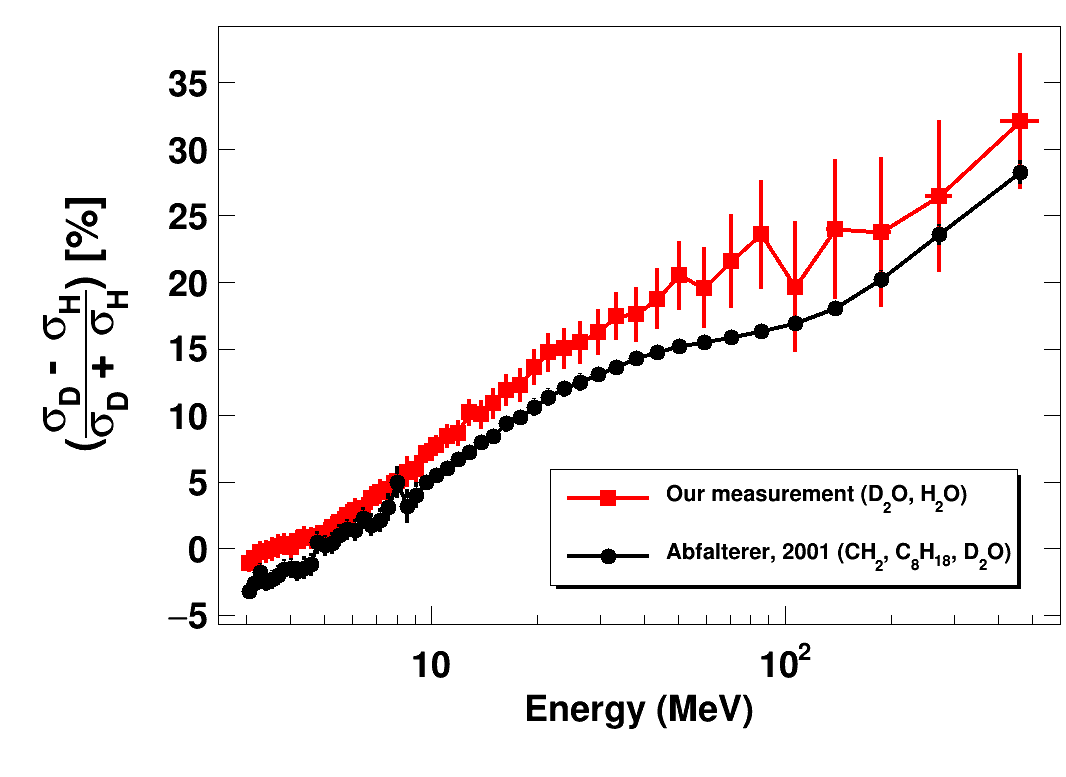
\includegraphics[width=0.9\textwidth]{figures/relativeDiff_DtoH.png}
    \caption[\tot\ relative difference between deuterium and hydrogen from our measurement]
    {The \tot\ relative difference between deuterium and hydrogen,
        as calculated by subtraction of our O \tot\ results from
        D$_{2}$O and H$_{2}$O. Data from our measurement are shown as red
        squares; the data of Abfalterer et al. \cite{Abfalterer1998} are shown
    as black circles.}
    \label{DtoH}
\end{figure}

\section{Results}
\subsection{Benchmarking \tot\ results with natural samples}
To validate our analysis, we first compared our \tot\ measurements on \cNat,
\niNat, \snNat, \pbNat\ against the high-precision data sets on natural samples from 
Finlay et al.\cite{Finlay1993} and Abfalterer et al.\cite{Abfalterer2001}, shown in Fig.
\ref{LiteratureBenchmarking}. From 3-100 \mega\electronvolt, our measurements are in excellent
agreement, within statistical error, with these previous data sets. Above 100 \mega\electronvolt, our results 
on natural samples diverge from the previous measurements,
(up to a relative difference of 5\% at 300 \mega\electronvolt\ for all 
samples), suggesting a small systematic effect at high energies when the instantaneous neutron 
flux is highest. To investigate this discrepancy, we analyzed data from multiple digitizer 
thresholds during data production, applied various software threshold, gated events by low- 
and high-integrated charge, and varied our software CFD logic, among other diagnostic tests. 
Throughout these exercises, the agreement
at $<$100 \mega\electronvolt\ and the discrepancy $>$100 \mega\electronvolt\ persisted.
To ensure the shift was not related to imprecision in the areal
density of the targets, we compared both our short and long natural carbon targets against 
each other (see Fig. \ref{CarbonBenchmarking}) and found excellent agreement: the relative 
difference was within 1\% throughout our energy domain, comparable to a similar test
conducted by Abfalterer et al. \cite{Abfalterer2001}. From Eq. \ref{CSCalculation},
it is clear that changes in flux ratio and sample areal
density can shift the calculated cross section up or down across the entire
energy range measured, but cannot change the \textit{slope} of the cross section
as energy is increased. Thus, the high-energy discrepancy is unlikely to be from
an incorrect monitor flux. Further, it was not dependent on the nuclear mass of
the sample nor with any other physical characteristics of the samples,
suggesting that backshine of neutrons into the flux monitor from the samples, or another 
physical mechanism, was not the cause.

Interestingly, we did not see any energy-dependent 
discrepancy in the \oSix\ results (see Fig. \ref{TwoPanelO}). Both our measurement and previous
measurements on O isotopes used compound samples (H$_{2}$O, D$_{2}$O, BeO, ZnO), so it is possible 
that the subtraction of the positive-ion species (D and H for us, Be and Zn for \cite{Finlay1993}), 
eliminated the energy-dependent systematic difference in our measurements.

\begin{figure}[tb]
    \centering
    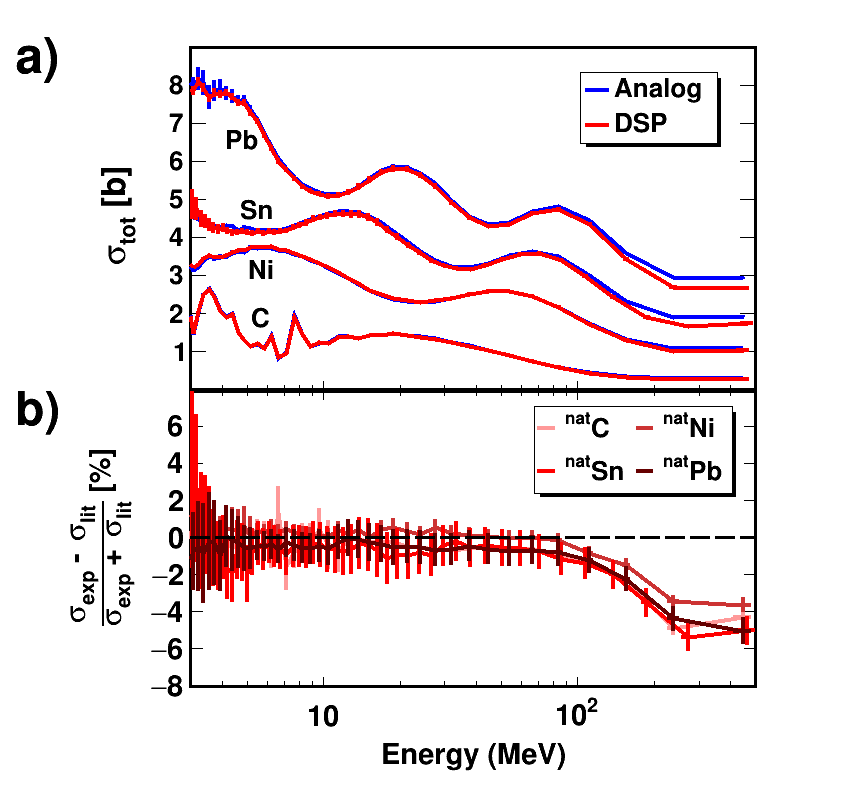
\includegraphics[width=0.9\textwidth]{figures/literatureBenchmarking.png}
    \caption[Comparison of our natural-sample \tot\ measurement against literature data]
    {
        A comparison of literature data (taken with analog
        techniques) and our results (signals processed with a digitizer, or
        ``DSP'')
        for natural C, Ni, Sn, and Pb. In panel (a), the absolute cross sections are shown from
        3-500 \mega\electronvolt; in panel (b), the relative differences between the literature data and
        our data are shown in percent. From 3-100 \mega\electronvolt, our data are fully consistent with the
        literature datasets but above 100 \mega\electronvolt, a relative difference arises, peaking at
        $\approx$5\% at 300 \mega\electronvolt.
    }
    \label{LiteratureBenchmarking}
\end{figure}

\begin{figure}[tb]
    \centering
    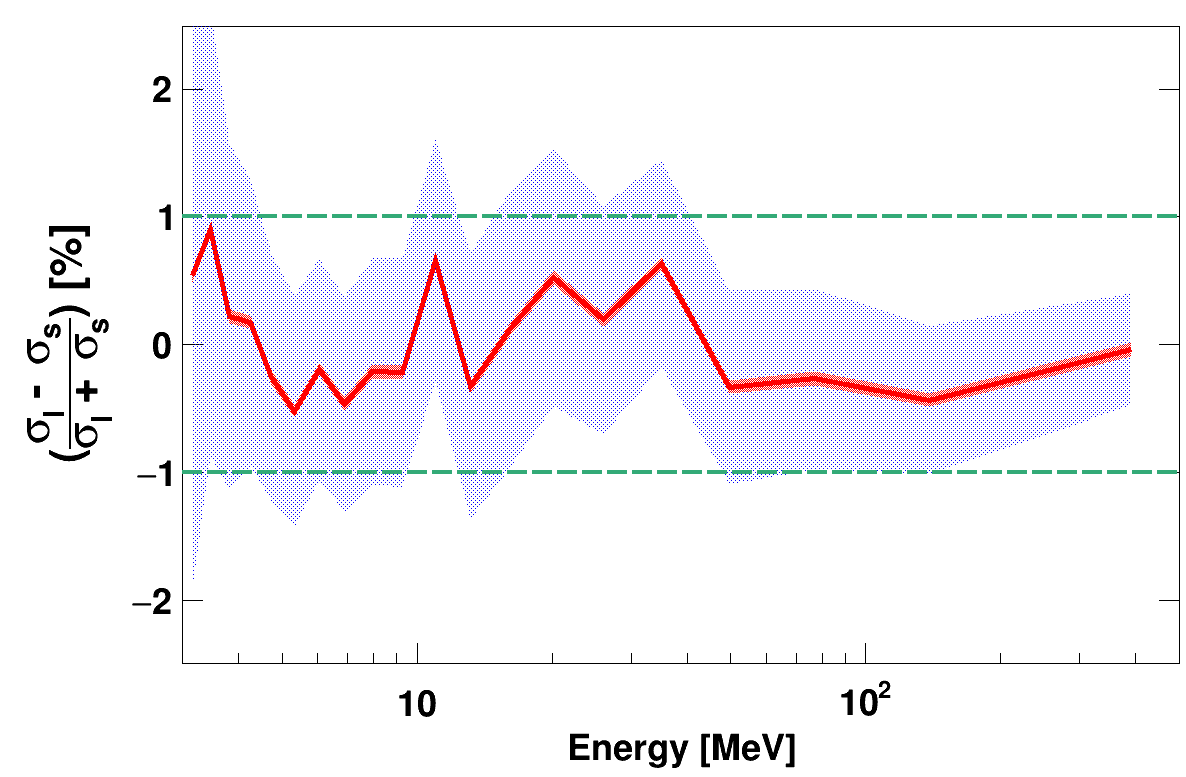
\includegraphics[width=0.9\textwidth]{figures/relativeDiff_longCarbonShortCarbon.png}
    \caption[Neutron \tot\ relative difference between short and long \cNat\ samples]
    {
        Relative difference of cross sections (red line) of
        our two lengths of \cNat, (27.3 mm and 13.7 mm), shown from 3-400
        \mega\electronvolt. Total error
        (including statistical and systematic) is indicated by the blue
        shaded region. Systematic error only (due to uncertainty in the areal
        density) is shown by the red shaded region (very small and immediately adjacent to 
        the red line). Clearly, statistical error dominates for this relative
        difference.
        Despite the low statistics of this diagnostic run (only 1.5 hours
        beam-on-target for each sample), the high efficiency of the
        digitizer-enabled approach means that the relative difference can be resolved to 
        $\pm$1\% for most of the energy range.
    }

    \label{CarbonBenchmarking}
\end{figure}

At neutron times-of-flight corresponding to energies $>$100 \mega\electronvolt, the number of
counts in the spectrum rises sharply as one moves to higher energies. In this
region, even a sub-nanosecond timing differences between the spectrum for the
blank and for the sample of interest is amplified into large errors in the
cross section calculation. Thus the event timing and data
storage routines must be kept completely ignorant of which target is currently
in-beam so as to avoid sample-dependent timing effects. In practice, this is
difficult, as acquisition with the blank sample is naturally associated with
a higher data rate as fewer neutrons are absorbed or scattered in-flight than during
with samples in the beam path. By reducing the rate of data acquisition
by an order of magnitude or more, the analog-electronics approach reduces the
absolute data rates of both the blank and the samples, mitigating this effect.
However, because much larger samples are required with the overall reduced data
rate, the relative data rate between the blank and samples is increased,
amplifying any effect on the electronics. Without a study of digital and analog
systems running simultaneously with input from the same detectors, it is not
clear which approach suffers more from this effect. Such a follow-up, especially
with multiple digitizers from differing manufacturers, would help
resolve the high-energy discrepancy we see between all of our \tot\ data sets
and literature data.

Our absolute \tot\ results for all isotopic targets are shown in Figs.
\ref{TwoPanelO}, \ref{TwoPanelNi}, \ref{TwoPanelRh}, and \ref{TwoPanelSn}.
All previous isotopic \tot\
measurements (where they exist) are shown alongside our results for comparison, and residuals 
between our data and literature data are provided in the lower panels. To make comparison 
meaningful, the literature
data sets shown have been modified to have the same bins as our data via a simple
linear interpolation of the original data bins. This rebinning
washes out the fine structure of the cross section data where the density of states
for a given sample is low and individual resonances are visible
(e.g., $^{\text{nat}}$C below 10 \mega\electronvolt). In all figures, error bars are indicated on data
points or are smaller than the size of the markers used.

Relative differences of our measured \tot\ between \oSixEight, \niEightFour, and
\snTwelveFour\ are shown in Figs. \ref{IsotopicDifferenceO}, \ref{IsotopicDifferenceNi}, 
and \ref{IsotopicDifferenceSn}, respectively. By examining relative differences between
isotopes, any systematic errors of our approach (besides the areal density uncertainties)
are divided out.

\subsection{\oSixEight\ \tot\ results}
Above 5 \mega\electronvolt, our \oSix\ \tot\ results are within 5\% of those from \cite{Finlay1993}, where
ZnO and BeO were used rather than H$_{2}$O. Below 5 \mega\electronvolt, the rapidly-rising
(n,p) cross section and resonance structure of Zn, Be, and \oSix\ contribute to
increased relative differences. Our measurement on \oEight\ extends the known
neutron \tot\ by over an order of magnitude and shows reasonable agreement to
the previous measurements taken over 50 years ago by \cite{Vaughn1965,Salisbury1965}.
Above 200 \mega\electronvolt, the \oEight\ \tot\ is smaller than the \oSix\ \tot\, a
consequence of the larger neutron elastic phase shift in \oEight\ compared to
\oSix, which pushes the \tot\ minimum to higher energies in \oEight.
\begin{figure}[tb]
    \centering
    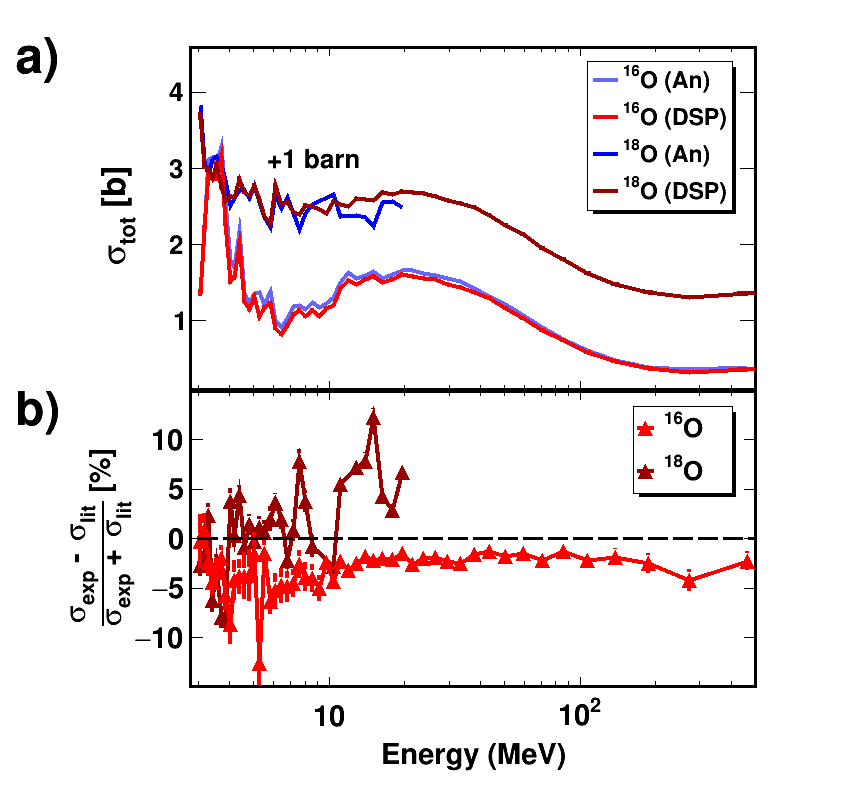
\includegraphics[width=0.9\textwidth]{figures/TwoPanelO.png}
    \caption[Neutron \tot\ for \oSixEight: our results and literature data]
    {Neutron \tot\ for \oSixEight: our results and literature data.
        (a) shows our digitizer-measured isotopic results (in shades of red) and
        corresponding analog-measured literature data \cite{Finlay1993, Perey1972, Vaughn1965,
        Salisbury1965} (in shades of blue). The data for \oEight\ have been
        shifted up by 1 barn for visibility.
        (b) shows the relative difference between our data
        and literature data that are shown in panel (a).
    }
    \label{TwoPanelO}
\end{figure}
\begin{figure}[tb]
    \centering
    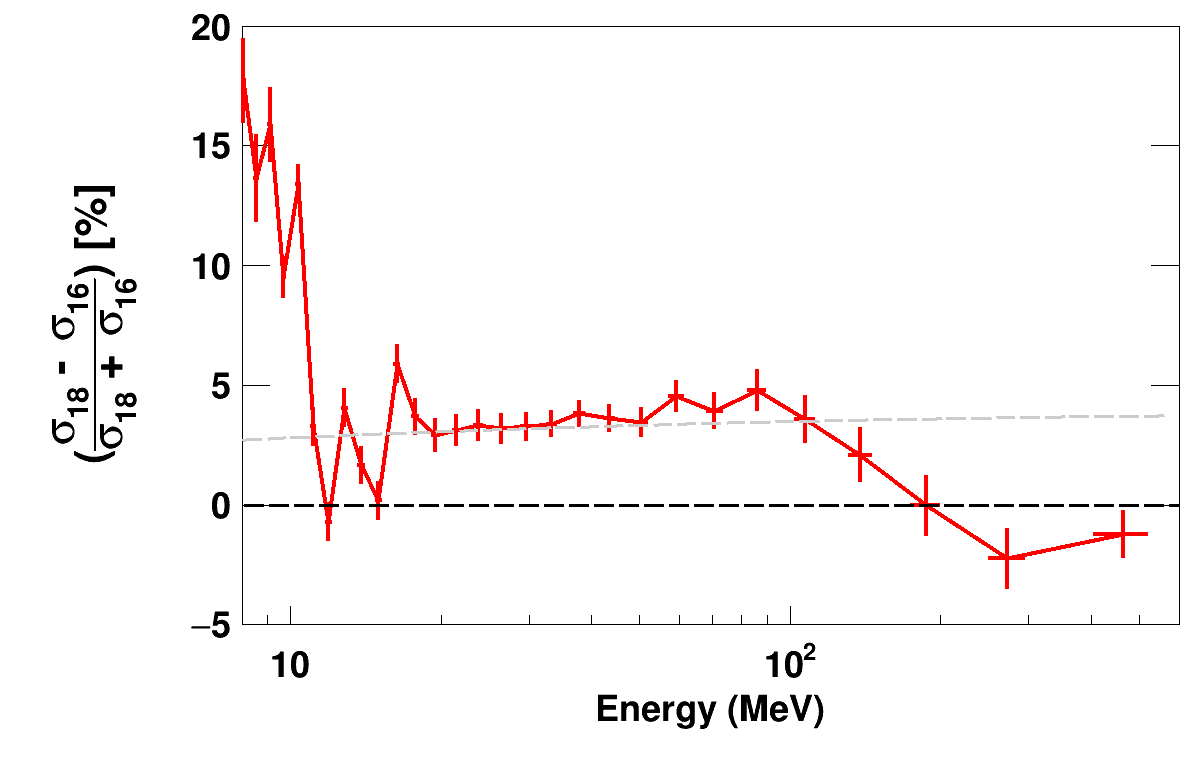
\includegraphics[width=0.9\textwidth]{figures/relativeDiff_O18O16.png}
    \caption[\oSixEight\ neutron \tot\ relative difference]
    {\oSixEight\ neutron \tot\ relative difference, from our newly-measured
        data sets (in red). Assuming a simple A$^{\frac{1}{3}}$ size scaling for the
        nuclear radius of \oEight\ from \oSix, the strongly-absorbing-sphere model 
        Eq. \ref{SASAbsolute} prediction for the \oSixEight\ neutron \tot\ relative
        difference is shown (black dashed line). From 10-100 \mega\electronvolt, the SAS
        model is surprisingly successful at reproducing the relative difference,
        though it fails above 100 \mega\electronvolt\ as the \oEight\ neutron \tot\ drops below
    that of \oSix.}
    \label{IsotopicDifferenceO}
\end{figure}

\subsection{\niEightFour\ \tot\ results}
In contrast to the case of O, no isotopic Ni data was available at all above 100
\mega\electronvolt, and high-precision literature data was only available up to 15 \mega\electronvolt\ for
\niEight\ \cite{Perey1993} and at only one point, 14.2 \mega\electronvolt, for \niFour\
\cite{Dukarevich1967}. Our results extended the energy range to 400 \mega\electronvolt\ and are
in good agreement with the previous results when their errors are included.
\begin{figure}[tb]
    \centering
    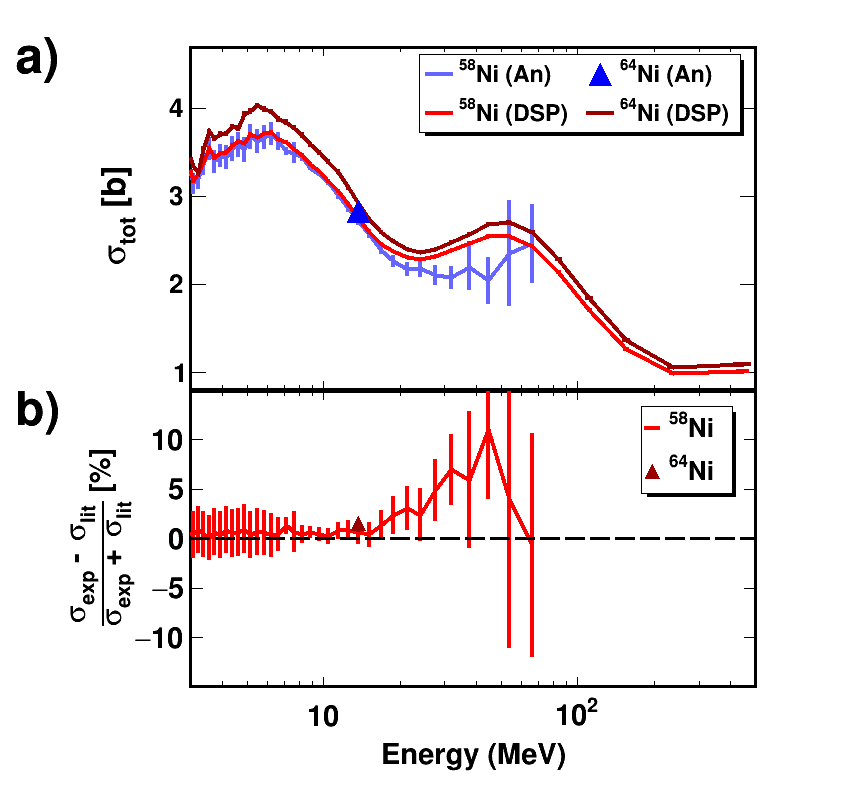
\includegraphics[width=0.9\textwidth]{figures/TwoPanelNi.png}
    \caption[Neutron \tot\ for \niEightFour: our results and literature data]
    {
        Neutron \tot\ for \niEightFour: our results and literature data.
        (a) shows our digitizer-measured isotopic results (in shades of red) and
        corresponding analog-measured literature data \cite{Perey1993,
        Dukarevich1967} (in shades of blue). (b) shows the relative difference
        between our data and literature data that are shown in panel a).
    }
    \label{TwoPanelNi}
\end{figure}
\begin{figure}[tb]
    \centering
    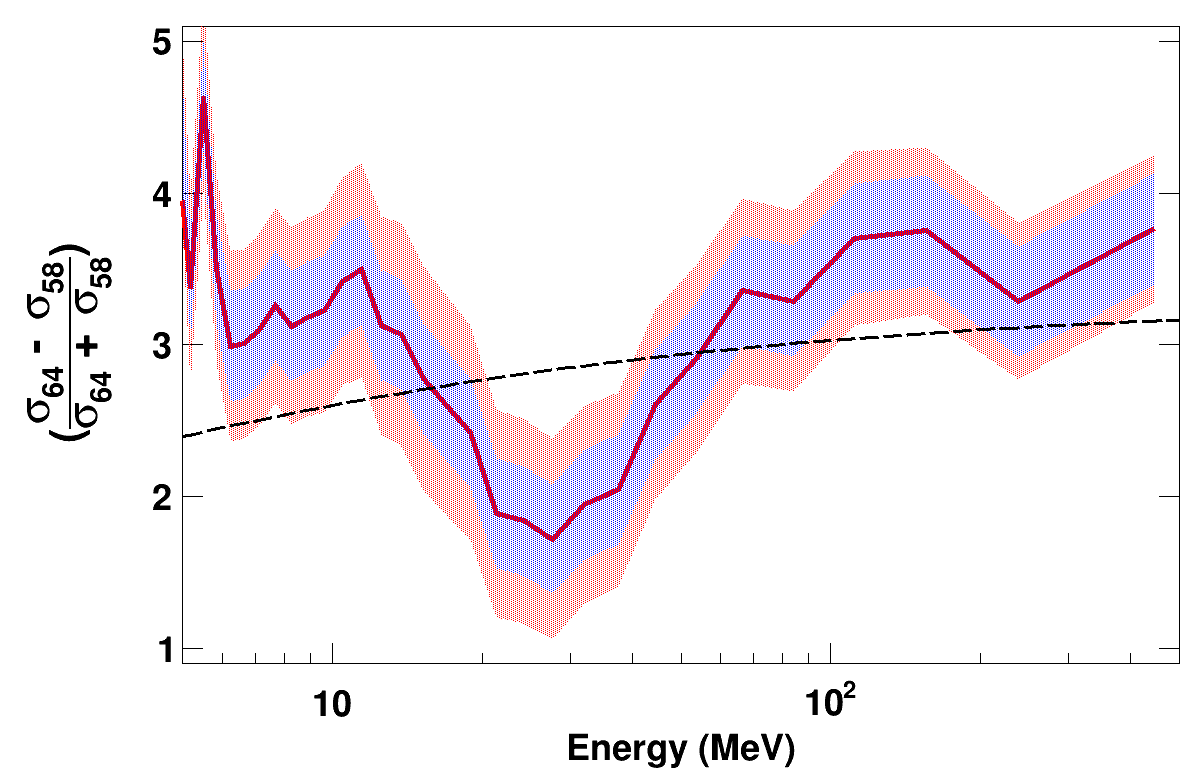
\includegraphics[width=0.9\textwidth]{figures/relativeDiff_Ni64Ni58.png}
    \caption[\niEightFour\ neutron \tot\ relative difference]
    {
        \niEightFour\ neutron \tot\ relative difference, from our newly-measured
        data sets (in red). Total error (including statistical and systematic)
        is indicated by the red shaded region. Systematic error only (due to
        uncertainty in the sample areal density) is shown by the blue shaded region.   
        Assuming a simple A$^{\frac{1}{3}}$ size scaling for the
        nuclear radius of \niFour\ from \niEight, the simple
        strongly-absorbing-sphere model Eq. \ref{SASAbsolute} prediction
        for the \niEightFour\ neutron \tot\ relative
        difference is shown (black dashed line).
    }
    \label{IsotopicDifferenceNi}
\end{figure}

\subsection{\rhThree\ \tot\ results}
The extremely small areal density and the reduced beam
time allotted for our \rhThree\ sample made it difficult to acquire sufficient statistics.
Nevertheless, by reducing the energy range and number of bins slightly, we were
able to achieve 1\% statistics for all bins and our results agree with those of
\cite{Poenitz1983} up to 20 \mega\electronvolt. Our results extend the known energy range by over an order of
magnitude up to 400 \mega\electronvolt.
\begin{figure}[tb]
    \centering
    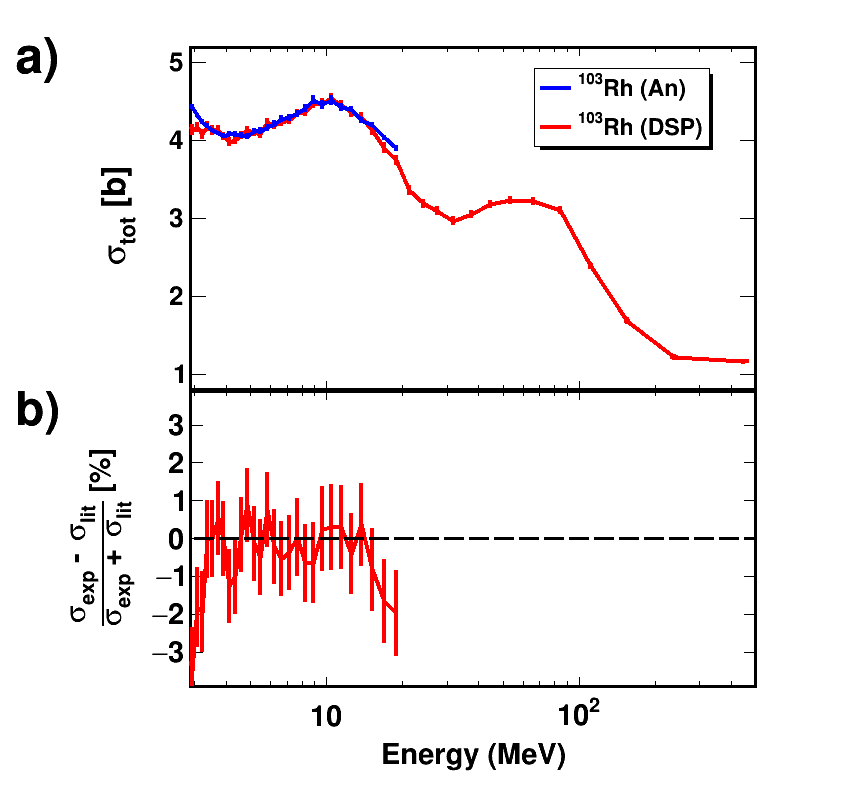
\includegraphics[width=0.9\textwidth]{figures/TwoPanelRh.png}
    \caption[Neutron \tot\ for \rhThree: our results and literature data]
    {
        Neutron \tot\ for \rhThree: our results and literature data.
        (a) shows our digitizer-measured isotopic results (in red) and
        corresponding analog-measured literature data \cite{Poenitz1983} (in blue).
        (b) shows the relative difference
        between our data and literature data that are shown in panel (a).
    }
    \label{TwoPanelRh}
\end{figure}

\subsection{\snTwelveFour\ \tot\ results}
Similar to Ni isotopes, the only existing Sn isotope neutron \tot\ data was at
low energies, up to 20 \mega\electronvolt\ for both \snTwelve\ and \snFour\ \cite{Harper1982, Timokhov1989, 
Rapaport1980, Dukarevich1967}. Our results extended the energy range to 400 \mega\electronvolt\ and are
in excellent agreement, $\approx$1\% difference, with the previous results.
\begin{figure}[tb]
    \centering
    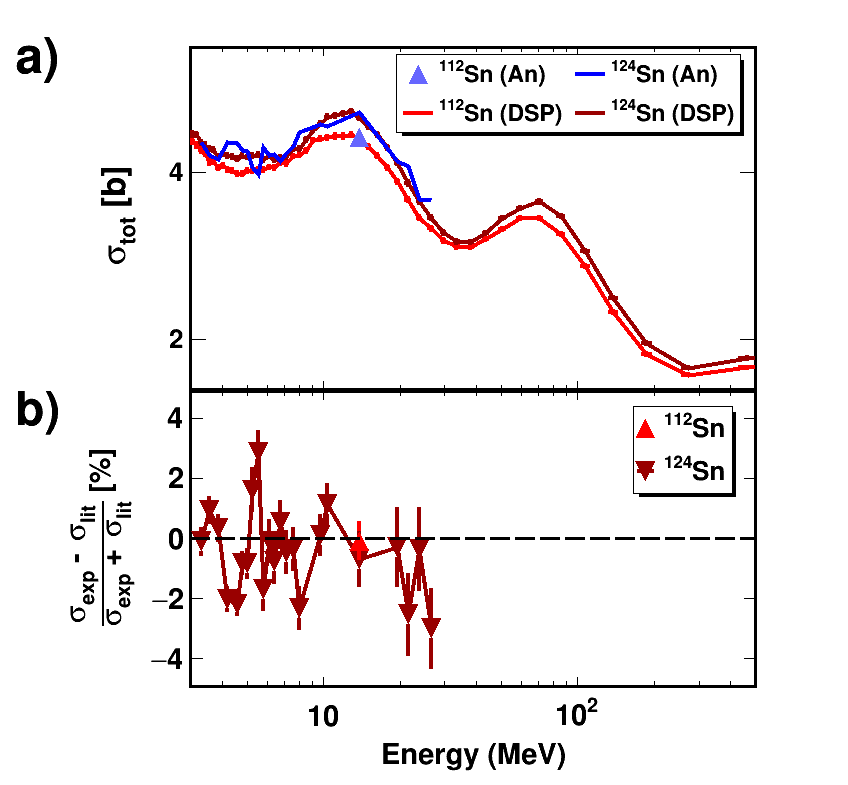
\includegraphics[width=0.9\textwidth]{figures/TwoPanelSn.png}
    \caption[Neutron \tot\ for \snTwelveFour: our results and literature data]
    {
        Neutron \tot\ for \snTwelveFour: our results and literature data.
        (a) shows our digitizer-measured isotopic results (in red) and
        corresponding analog-measured literature data \cite{Harper1982, Timokhov1989, 
        Rapaport1980, Dukarevich1967} (in shades of blue).
        (b) shows the relative difference between our data
        and literature data that are shown in panel (a). The data sets are in
        excellent agreement where literature data exist, up to 20 \mega\electronvolt.
    }
    \label{TwoPanelSn}
\end{figure}
\begin{figure}[tb]
    \centering
    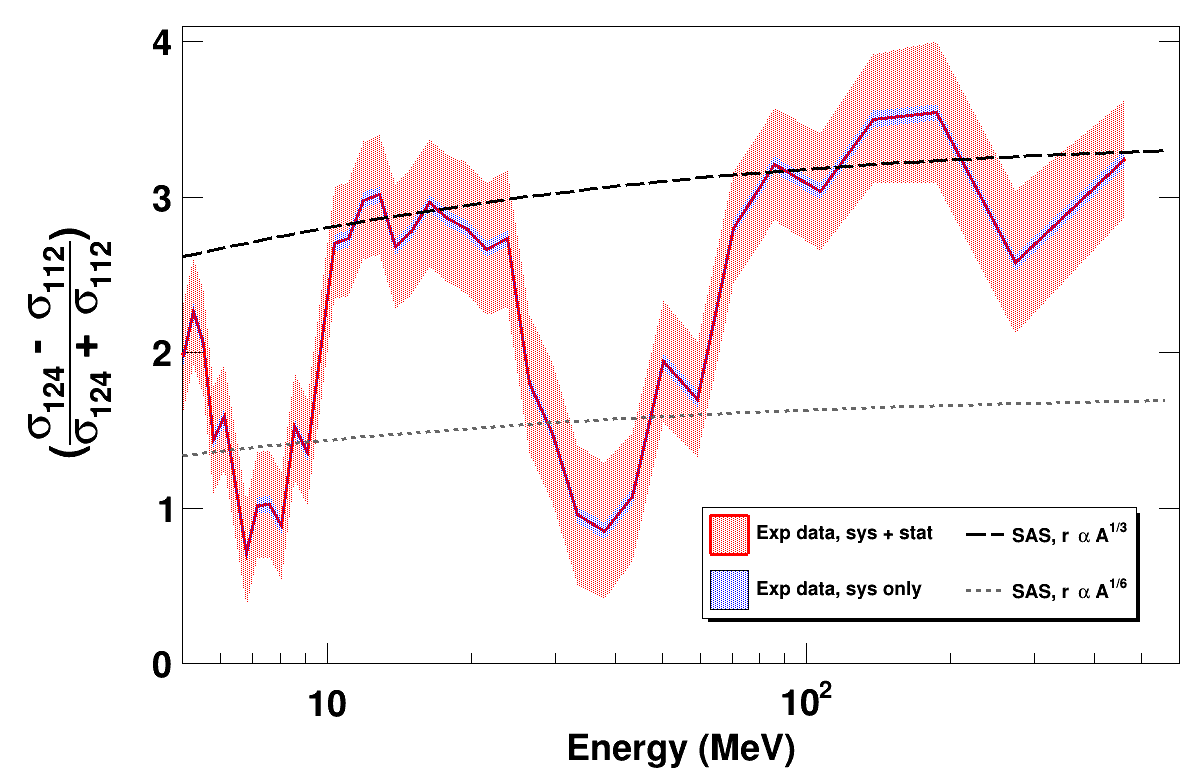
\includegraphics[width=0.9\textwidth]{figures/relativeDiff_Sn124Sn112.png}
    \caption[\snTwelveFour\ neutron \tot\ relative difference]
    {
        \snTwelveFour\ neutron \tot\ relative difference, from our newly-measured
        data sets (in red). Total error (including statistical and systematic)
        is indicated by the red shaded region. Systematic error only (due to
        uncertainty in the sample areal density) is shown by the blue shaded region.   
        The predictions of the simple strongly-absorbing-sphere model of
        Eq. \ref{SASAbsolute} for the \snTwelveFour\ neutron \tot\ relative
        difference are shown for two nuclear radius size scalings: $r \alpha A^{\frac{1}{3}}$
        (black dashed line) and $r \alpha A^{\frac{1}{6}}$
        (cf. the observed $A^{\frac{1}{6}}$ scaling of the Sn isotope shift in Fig.
        \ref{SnIsotopeShift}).
    }
    \label{IsotopicDifferenceSn}
\end{figure}

\afterpage{\clearpage}


\chapter{Neutron Elastic Cross Sections: Experiment} \label{ECSExperiment}
\section{Overview of neutron \el\ experiments}
In neutron elastic scattering measurements, the same time-of-flight techniques are used:
given a ``starting gun'' when neutrons are produced and the neutron arrival time
at a time-of-flight detector, the neutron energy can be calculated.
However, in contrast to total cross section measurements, neutron elastic scattering
measurements require a monoenergetic neutron beam so that elastically-scattered
neutrons can be isolated. Unlike transmission measurements (e.g., total cross
sections), which measure the neutron scattering integrated
over all solid angles, neutron \el\ cross sections are measured differentially with respect to 
solid angle. To measure the angular dependence, one or more time-of-flight detectors
are moved around the scattering sample on a large goniometer. As the differential cross section 
drops precipitously at large scattering angles, more beam time must be spent at
large angles to generate sufficient statistics.

In transmission measurements, the time-of-flight detector is typically placed
very far from the scattering sample so that it subtends an extremely small solid
angle so that only unscattered particles are detected.
For example, in the neutron \tot\ experimental setup described in Chapter
\ref{TCSExperiment}, the scintillator of the time-of-flight detector subtended
4.5$\times$10$^{-6}$ steradians from the point of view of the samples. Thus, the
contribution to background from isotropic $\gamma$-ray production in the samples is negligible.
In differential measurements,
background from $\gamma$-ray production in the samples may exceed the signal
from elastically-scattered neutrons, especially at backward angles where the elastic
cross section is lowest. Pulse-shape discrimination (\gls{PSD})
techniques must be used to filter out 
$\gamma$ rays, leaving only events from elastically-scattered neutrons.

\subsection{Pulse-Shape Discrimination (PSD)}
To identify neutron- and gamma-induced detector events, pulse-shape discrimination
relies on the different modes of energy deposition in neutrons and $\gamma$ rays.
A liquid scintillator must be used that exhibits prompt fluorescence with a
lifetime of a few \nano\second\ (from a singlet
state) and delayed phosphorescence with much longer lifetime in the
\micro\second\ range or longer (from a triplet state). Figure \ref{JablonskiExample} shows the
relevant level structure for such a molecule. During a scattering experiment,
incident neutrons deposit energy by collision with scintillator nuclei.
These recoiling nuclei (mostly protons) decelerate rapidly in the scintillating
medium via Coulombic interactions with all electrons in the vicinity,
exciting many scintillator molecules in the
ion track. In contrast, incident $\gamma$ rays interact primarily with
single atomic electrons, which, during their recoil, produce a lower excitation energy density.
For the same total energy deposition,
neutron-initiated events produce a higher 
concentration of excited scintillator molecules than do $\gamma$-ray-initiated
events.

In each population of excited scintillator molecules, most molecules are in a
singlet excited state, and they decay promptly by fluorescence back to the
ground state. A small fraction remain in a triplet excited state,
either due to their initial excitation to a
triplet state or because of intersystem crossing from a singlet state. Kept isolated, these
triplet-state molecules have lifetimes that are orders of magnitude longer
(\micro\second\ to \milli\second) than the those in a singlet state because of the required spin
flin to return to the ground-state manifold. If, however, two nearby triplet-state
molecules collide and exchange a unit of spin, they can convert to two singlet-state
molecules, one in the ground-state manifold and one in an excited-state manifold. The excited
singlet-state molecule will decay promptly (\nano\second), freed of quantum-mechanical forbiddenness.
Thus, after the initial prompt fluorescence, delayed light output will appear tens
of \nano\second\ later from these triplet-triplet fusion events. The amount of light will be
dependent on the rate of triplet-triplet collision, a second-order kinetics
process associated with the diffusion of excited scintillator molecules in the
medium. For neutron-initiated events, where the concentration of excited molecules is
higher, the delayed light output is correspondingly higher than for $\gamma$-ray-initiated
events. By comparing the tail of the light output signal to the prompt
fluorescence peak, neutrons and $\gamma$-rays can be distinguished. Typically, the differences in
light output are quantified by comparing the integrated charge of the prompt fluorescence peak
with the integrated charge of a section of the delayed fluoresence. Machine learning 
techniques have also been applied to light output data to further improve discrimination 
\cite{Doucet2018} beyond the simple charge-gate-ratio method. Recently, pulse-shape
discrimination has been shown to be possible in certain solid organic crystals (e.g.,
para-terphenyl, which is also used in laser dyes).

\begin{figure}[tb]
    \centering
    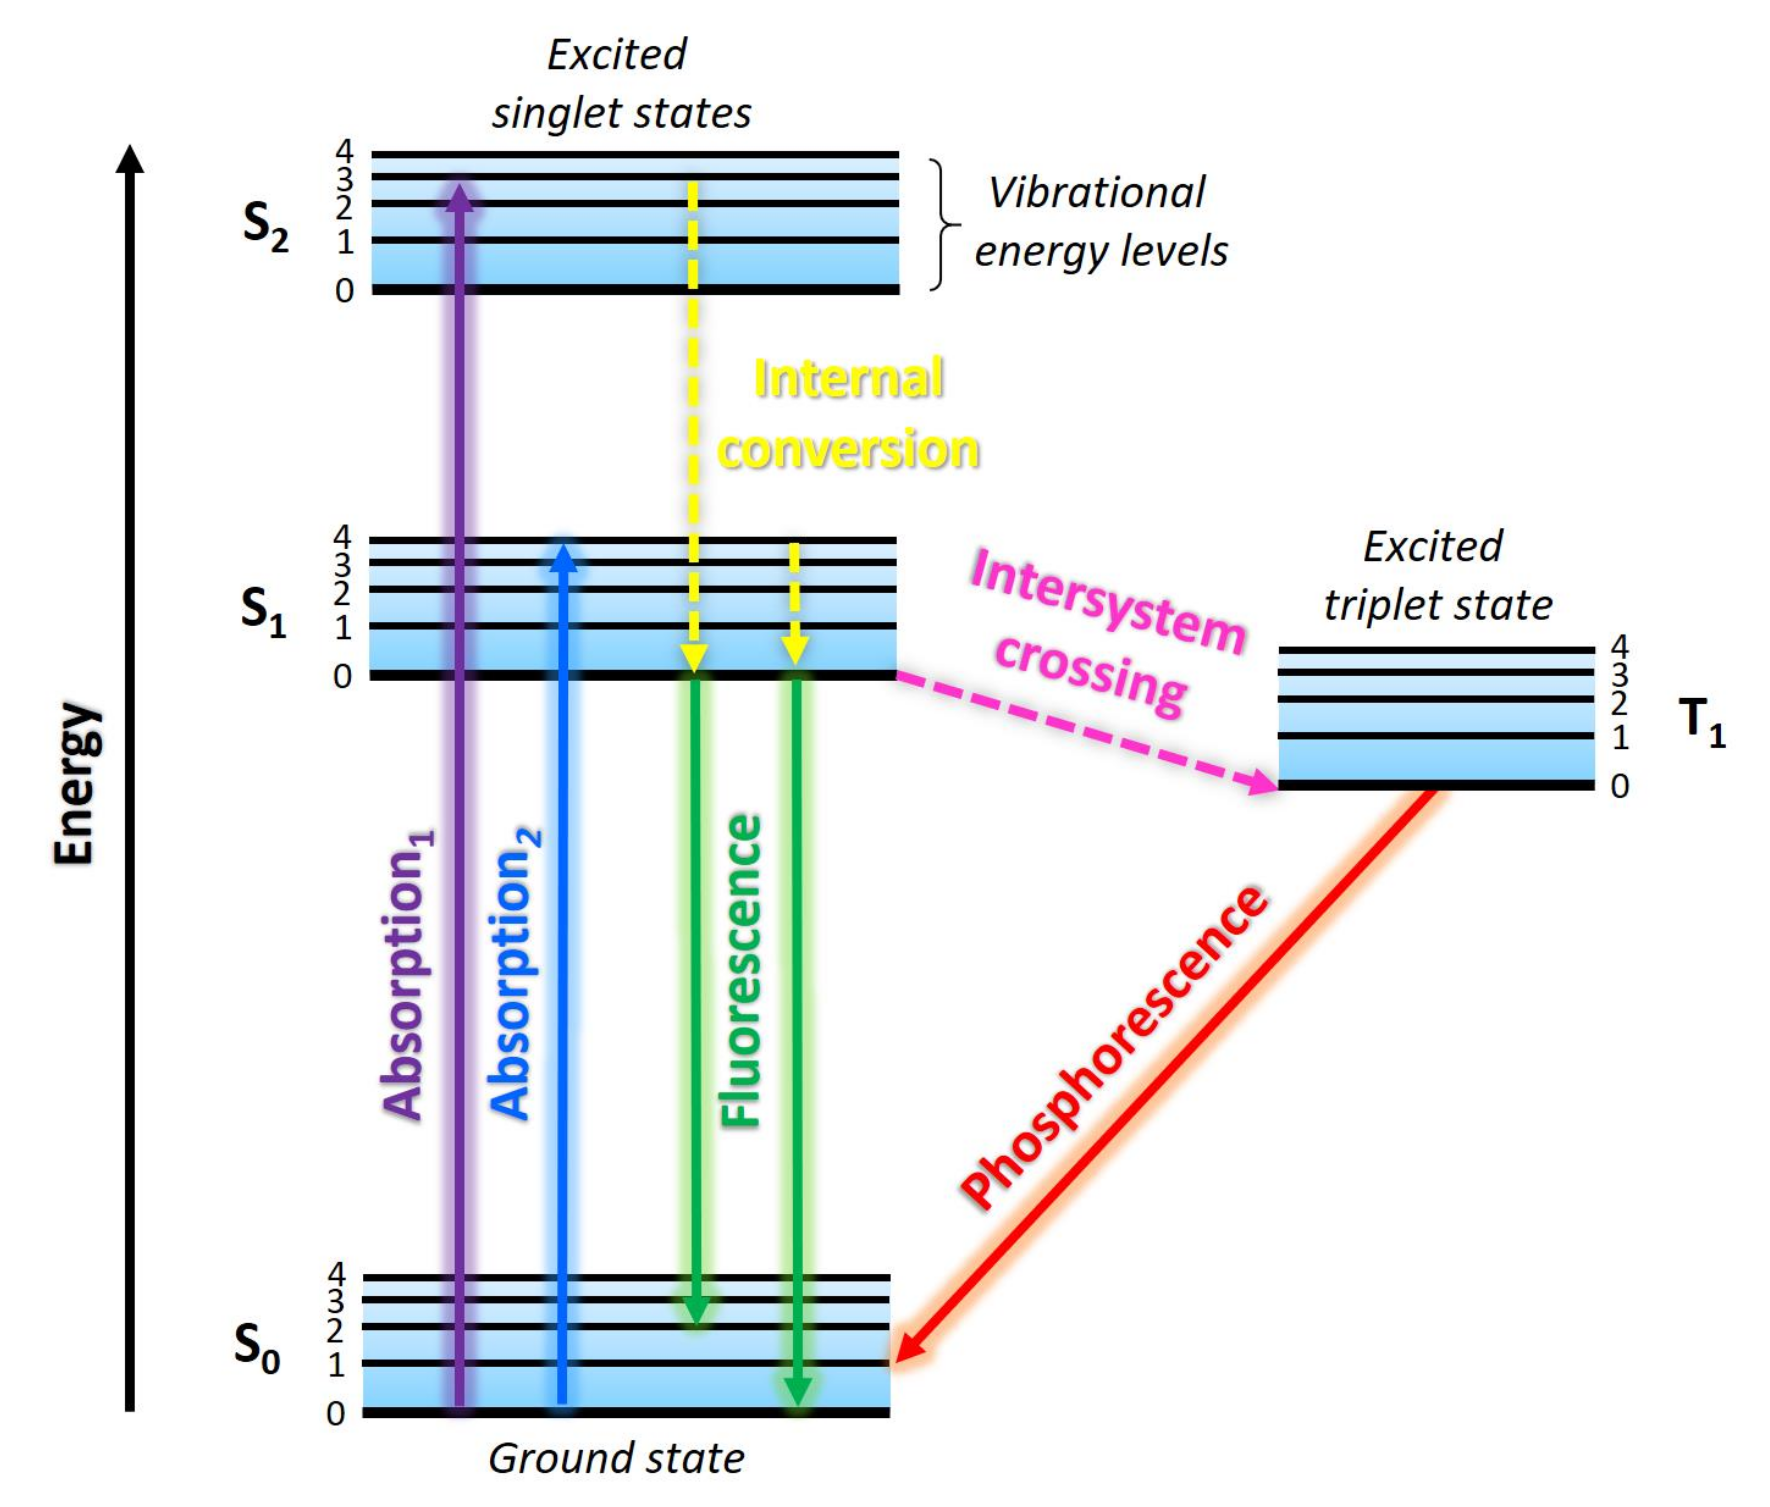
\includegraphics[width = 0.9\textwidth]{figures/JablonskiExample_KangDissertation.png}
    \caption[Example Jablonski diagram for organic scintillator]
    {
        Example Jablonski diagram for an organic scintillator used for
        pulse-shape discrimination. After initial excitation to a higher
        electronic manifold, energy is shed non-radiatively by internal
        conversion on the picosecond timescale. If the first vibrational state of the S1
        manifold is reached, rapid decay to the S0 manifold occurs on the
        \nano\second\ timescale. Alternatively, the system may undergo intersystem
        crossing to the T1 manifold, where it reaches the lowest vibrational
        state. The T1-S0 transition is quantum-mechanically-forbidden,
        dramatically increasing the lifetime of the T1 state and leading to
        delayed light output, or phosphorescence. Figure used with permission 
        from J. Kang \cite{KangPhDThesis}. 
    }
    \label{JablonskiExample}
\end{figure}

In our \snTwelveFour\ neutron \el\ cross section measurements presented below,
we used both \gls{PSD} data of this kind and the pulse height of each
event to segregate neutrons from $\gamma$-rays (see Figure \ref{PHPSDPlot} in Chapter
\ref{ECSAnalysis}). Our approach follows similar neutron \el\ measurements
conducted at the Triangle University Nuclear Laboratory (\gls{TUNL}) over the last three decades,
including a measurement on \snTwenty\ at 17 \mega\electronvolt\ conducted by Guss et al.
\cite{Guss1989, GussPhDThesis} to which we later compare our results on
\snTwelveFour.

\section{Sample Preparation}
The same \snTwelveNatFour\ samples used in the neutron \tot\ experiment (see Chapter
\ref{TCSExperiment}) were used for our neutron
\el\ measurements without modification. Two additional samples, one of graphite and one
polyethylene, were provided by the TUNL facility in order to normalize our \el\
results using the extremely-well-known (n,p) elastic cross section. The
details of this normalization are given in Chapter \ref{ECSAnalysis}.
The physical characteristics of all the samples are given in Table \ref{ECSSampleTable}.

\begin{table}[ht]
    \caption[Physical characteristics of samples used for neutron \el\
    measurements]
    {
        Physical characteristics of samples used for the neutron \el\
        measurements. For isotopically-enriched samples, the natural abundance
        of the enriched isotope and the isotopic fraction of the sample are
        given.
    }
    \label{ECSSampleTable}
    \begin{center}
        \begin{tabular}{ c c c c c c c }
            \hline
            Isotope & Length & Diameter
            & Mass & Nat. Abund. & Sample Purity\\
                 & [mm] & [mm] & [g] & [\%] & [\%]\\
            \hline

            $^{\text{nat}}$C & 23.58 & 9.39 & 2.924 & - & -\\
            (CH$_{2}$)$_{n}$ & 22.70 & 14.18 & 3.389 & - & -\\

            $^{112}$Sn & 13.65(3) & 8.245(5) &
            4.9720 & 0.97 & 99.9\\
            $^{\text{nat}}$Sn & 13.68(3) & 8.245(5) &
            5.3263 & - & -\\
            $^{124}$Sn & 13.73(3) & 8.245(5) &
            5.5492 & 5.79 & 99.9\\

            \hline
        \end{tabular}
    \end{center}
\end{table}

\section{Experimental Facility at TUNL}
We conducted our neutron \el\ measurements at the neutron TOF
beamline at TUNL (diagrammed in Fig. \ref{ExperimentalSetupTUNL}) in 2017 and 2018.
Incident deuterons, supplied by the
facility's variable-energy tandem Van de Graaff accelerator, impinged on a deuterium
gas cell to produce a forward-focused neutron beam via the d(d,n)$^{3}$He
reaction. This exothermic reaction has a Q-value of 3.269 \mega\electronvolt.
Two measurements, one for 11 \mega\electronvolt\
neutrons and one for 17 \mega\electronvolt\ neutrons, were
conducted. The gas cell pressure varied between 35-40 psi during our
measurement. Per \cite{GussPhDThesis}, we estimate a neutron beam energy spread
at the sample position of 350 keV, mostly from deuterium beam straggling
in the gas cell prior to reacting. The deuterium gas cell
was backed with a fresh tantalum beam stop to prevent unreacted deuterons from
reaching the samples. Based on the number of counts collected during the
normalization runs described below, we estimated that the average neutron flux incident
on the sample was $\approx5\times10^{6}$ neutrons\per\second\ for the 11 MeV run
in 2017 and $\approx1\times10^{7}$ neutrons\per\second for the 17 MeV run in
2018. Of course, the instantaneous neutron flux is much higher due to the pulse
structure of the beam.

The production samples (\snTwelve, \snFour, and a blank) were suspended several
\centi\meter\ downstream of the gas cell in a vertically-aligned wire basket apparatus.
In addition to the production runs, a few normalization runs were taken
with the TUNL-supplied samples (graphite, polyethylene, and a blank).
Between runs, samples were rotated into position
with a hand-actuated pulley. Sample alignment with the gas cell was confirmed
by transit. Neutrons scattering off the samples were recorded by one
of the two main time-of-flight
detectors, designated ``4M'' and ``6M'', roughly 4 and 6 meters away from the target.
These detectors were mounted on large, movable carriages, or ``arms'',
that could be rotated to different angles independently so that two angular
measurements could be conducted simultaneously. By recessing the detectors deep within
the arms' heavy shielding, only neutrons entering the arm at a precise angle
were counted. The active volumes of the 4M and 6M detectors were composed of
NE218 organic liquid scintillator capable of PSD.

To further reduce room background and to screen direct neutrons the gas cell,
an ensemble of ``shadow bars'' (wedge-shaped tungsten bricks)
were used to adjust the aperture at the entrance to the arms. After an arm's
angle was changed, the shadow bars were aligned by hand so that the
detector within the arm had no line-of-sight to the gas cell or the
shielding of the other arm. Any configuration in which the arms were in opposition (i.e., the
angle between the arms was 180$\pm$20 degrees) could allow neutrons scattered
from one arm to enter the detector of the other arm, so these configurations were avoided.

Besides the time-of-flight detectors installed in the arms, a ceiling monitor
detector (CMON) and zero-degree detector aligned with the beam (ZDEG) were used
to record beam flux. In addition, a capacitive pickoff signal
from the accelerator was collected to serve as a time-of-flight
(TOF) stop signal any time an event was recorded on one of the four neutron
detectors. Prior to production, detectors were gain-matched and calibrated with $^{137}$Cs
and $^{22}$Na sources using the Compton edges produced from these $\gamma$-ray sources. For the
4M (6M) detector, a time resolution of 2 ns (3 ns) was achieved.
An exhaustive description of the TUNL TOF room geometry, detector characteristics,
gas cell, and other apparatus considerations is provided in \cite{GussPhDThesis}.
\begin{figure}[tb]
    \centering
    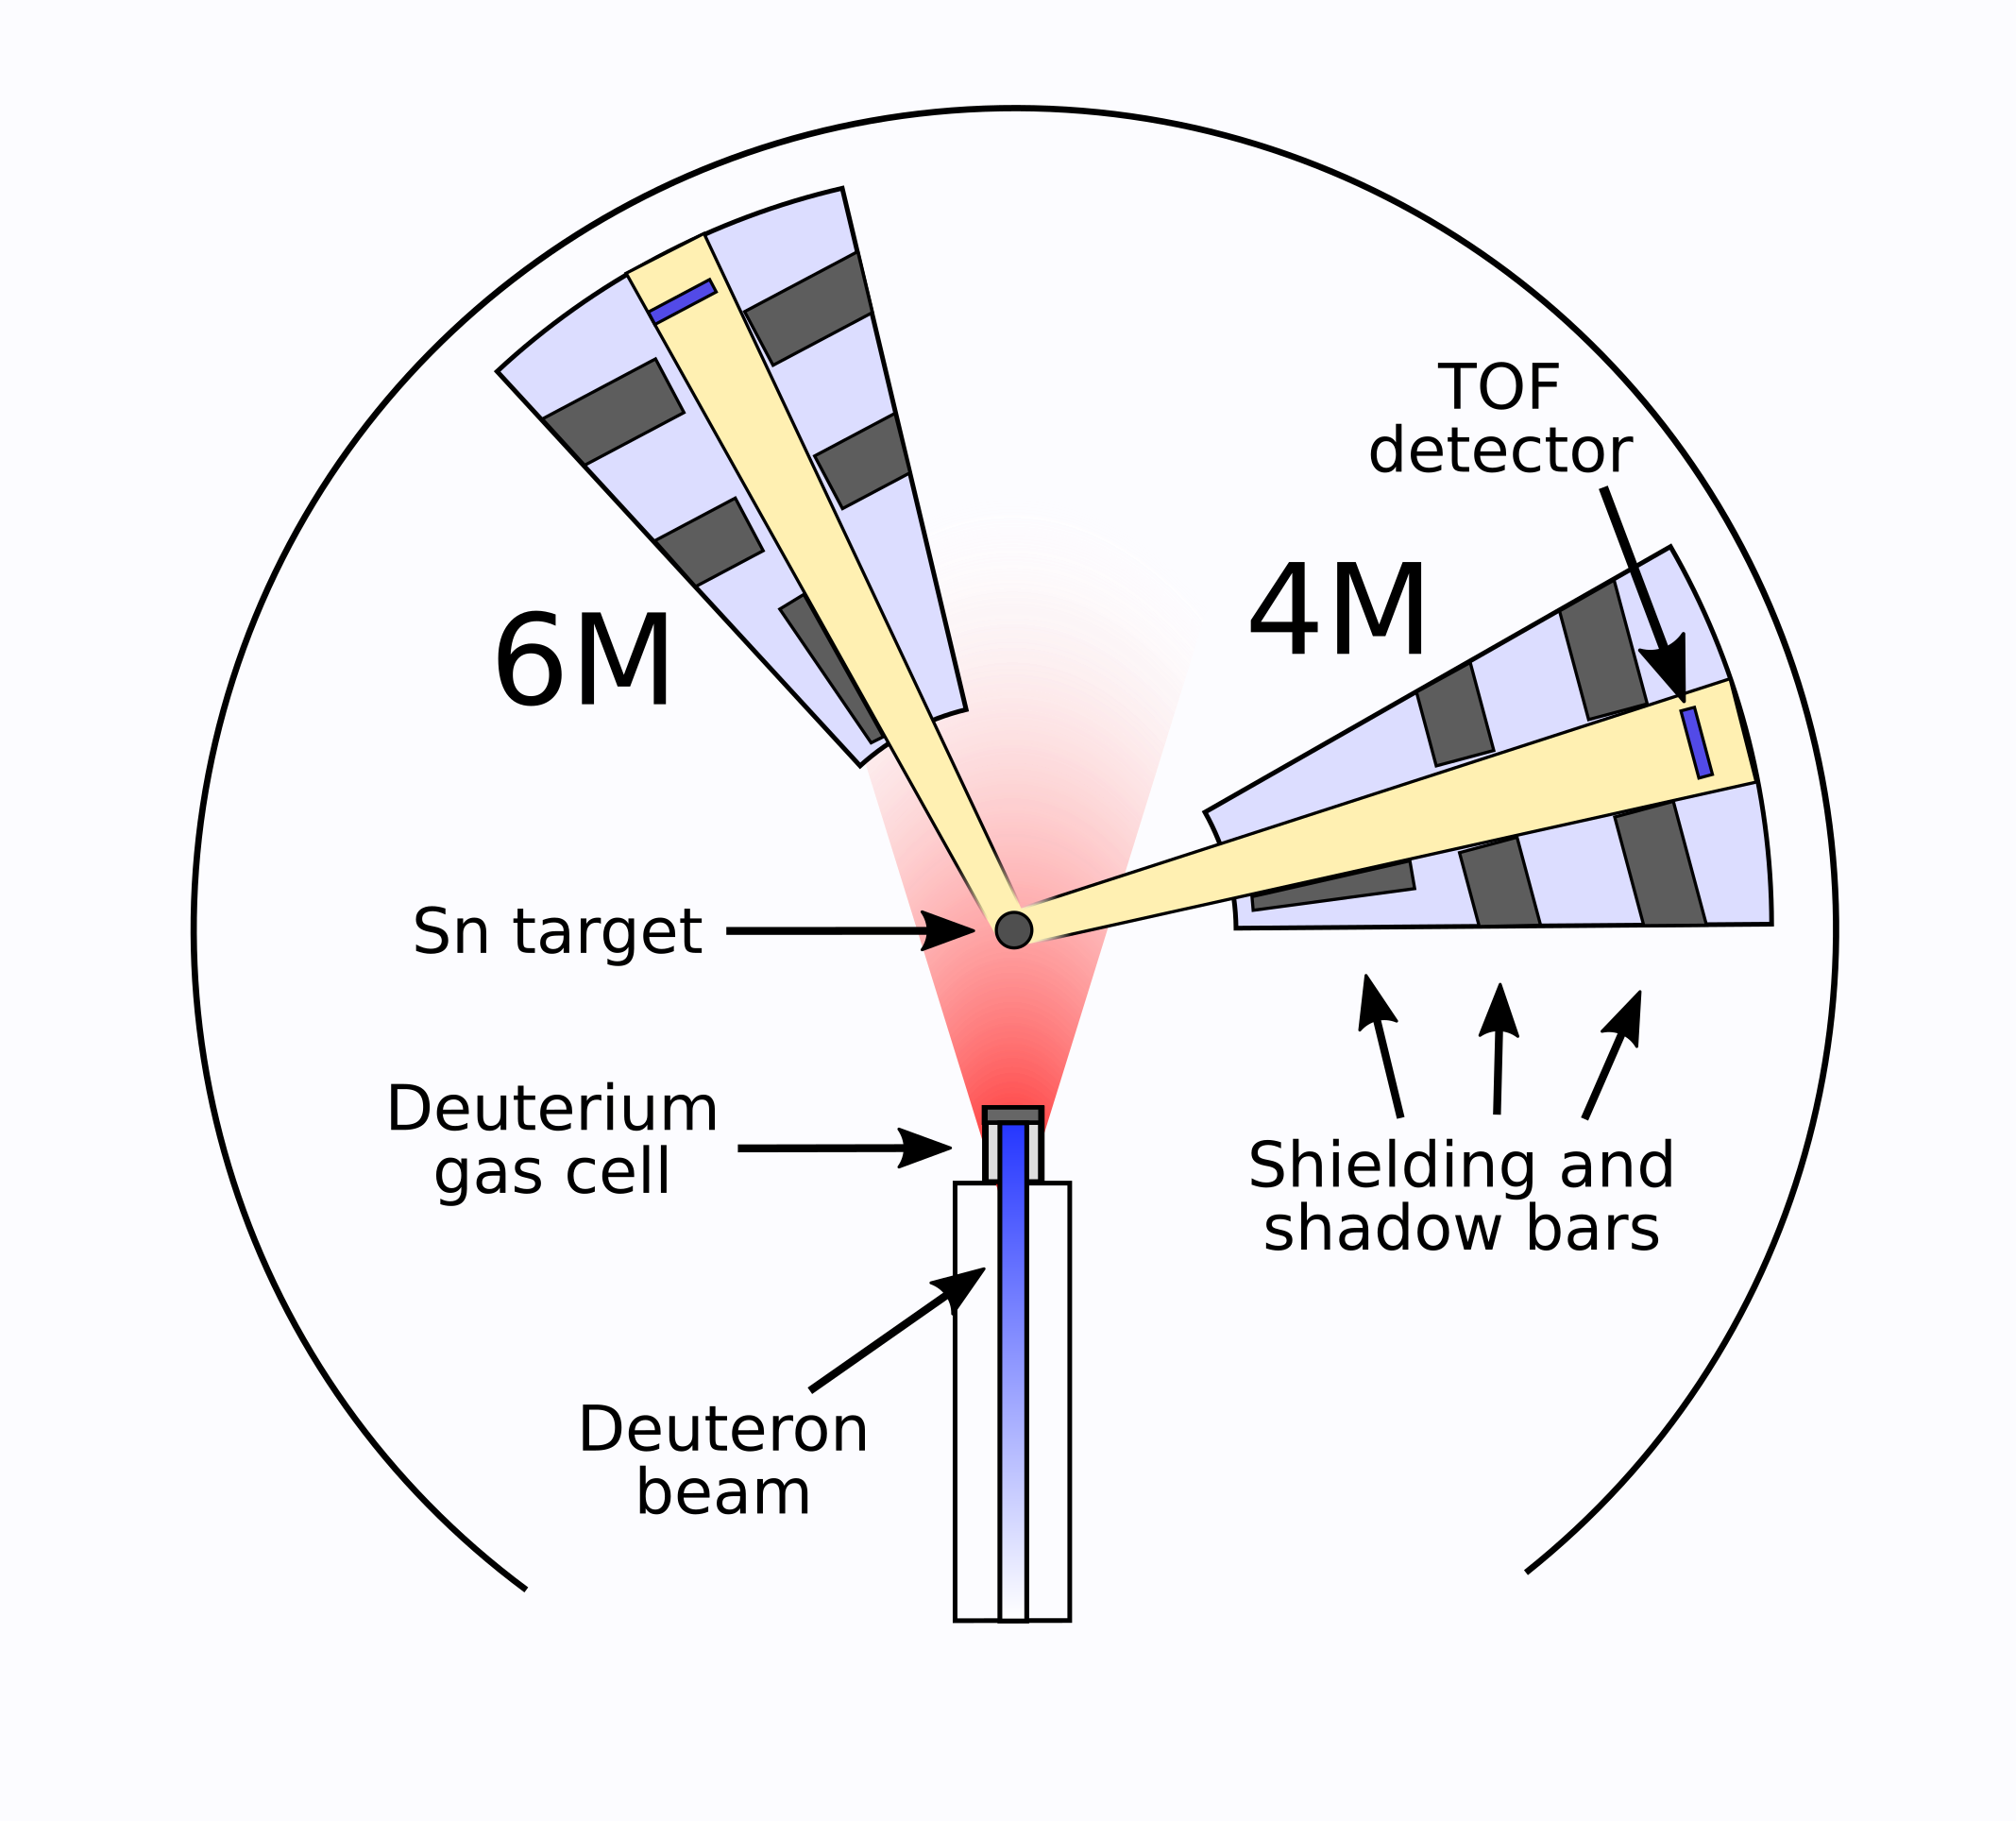
\includegraphics[width = 0.9\textwidth]{figures/ExperimentalSetupTUNL.png}
    \caption[Diagram of the neutron TOF room at TUNL] 
    {
        Diagram of the neutron TOF room at TUNL. Neutrons are produced by d(d,n)$^{3}$He reaction in
        a small gas cell, forming a forward-focused cone (in red). They scatter
        off the sample into one of the detector arms, labeled 4M and 6M, where the neutron
        times-of-flight are recorded. Another shielded detector (not pictured), suspended from the 
        ceiling, serves as a flux monitor so that absolute cross sections can be
        recovered. The angle of each detector arm is read from a goniometer in
        the center of the room.
    }
    \label{ExperimentalSetupTUNL}
\end{figure}

\begin{figure}[tb]
    \centering
    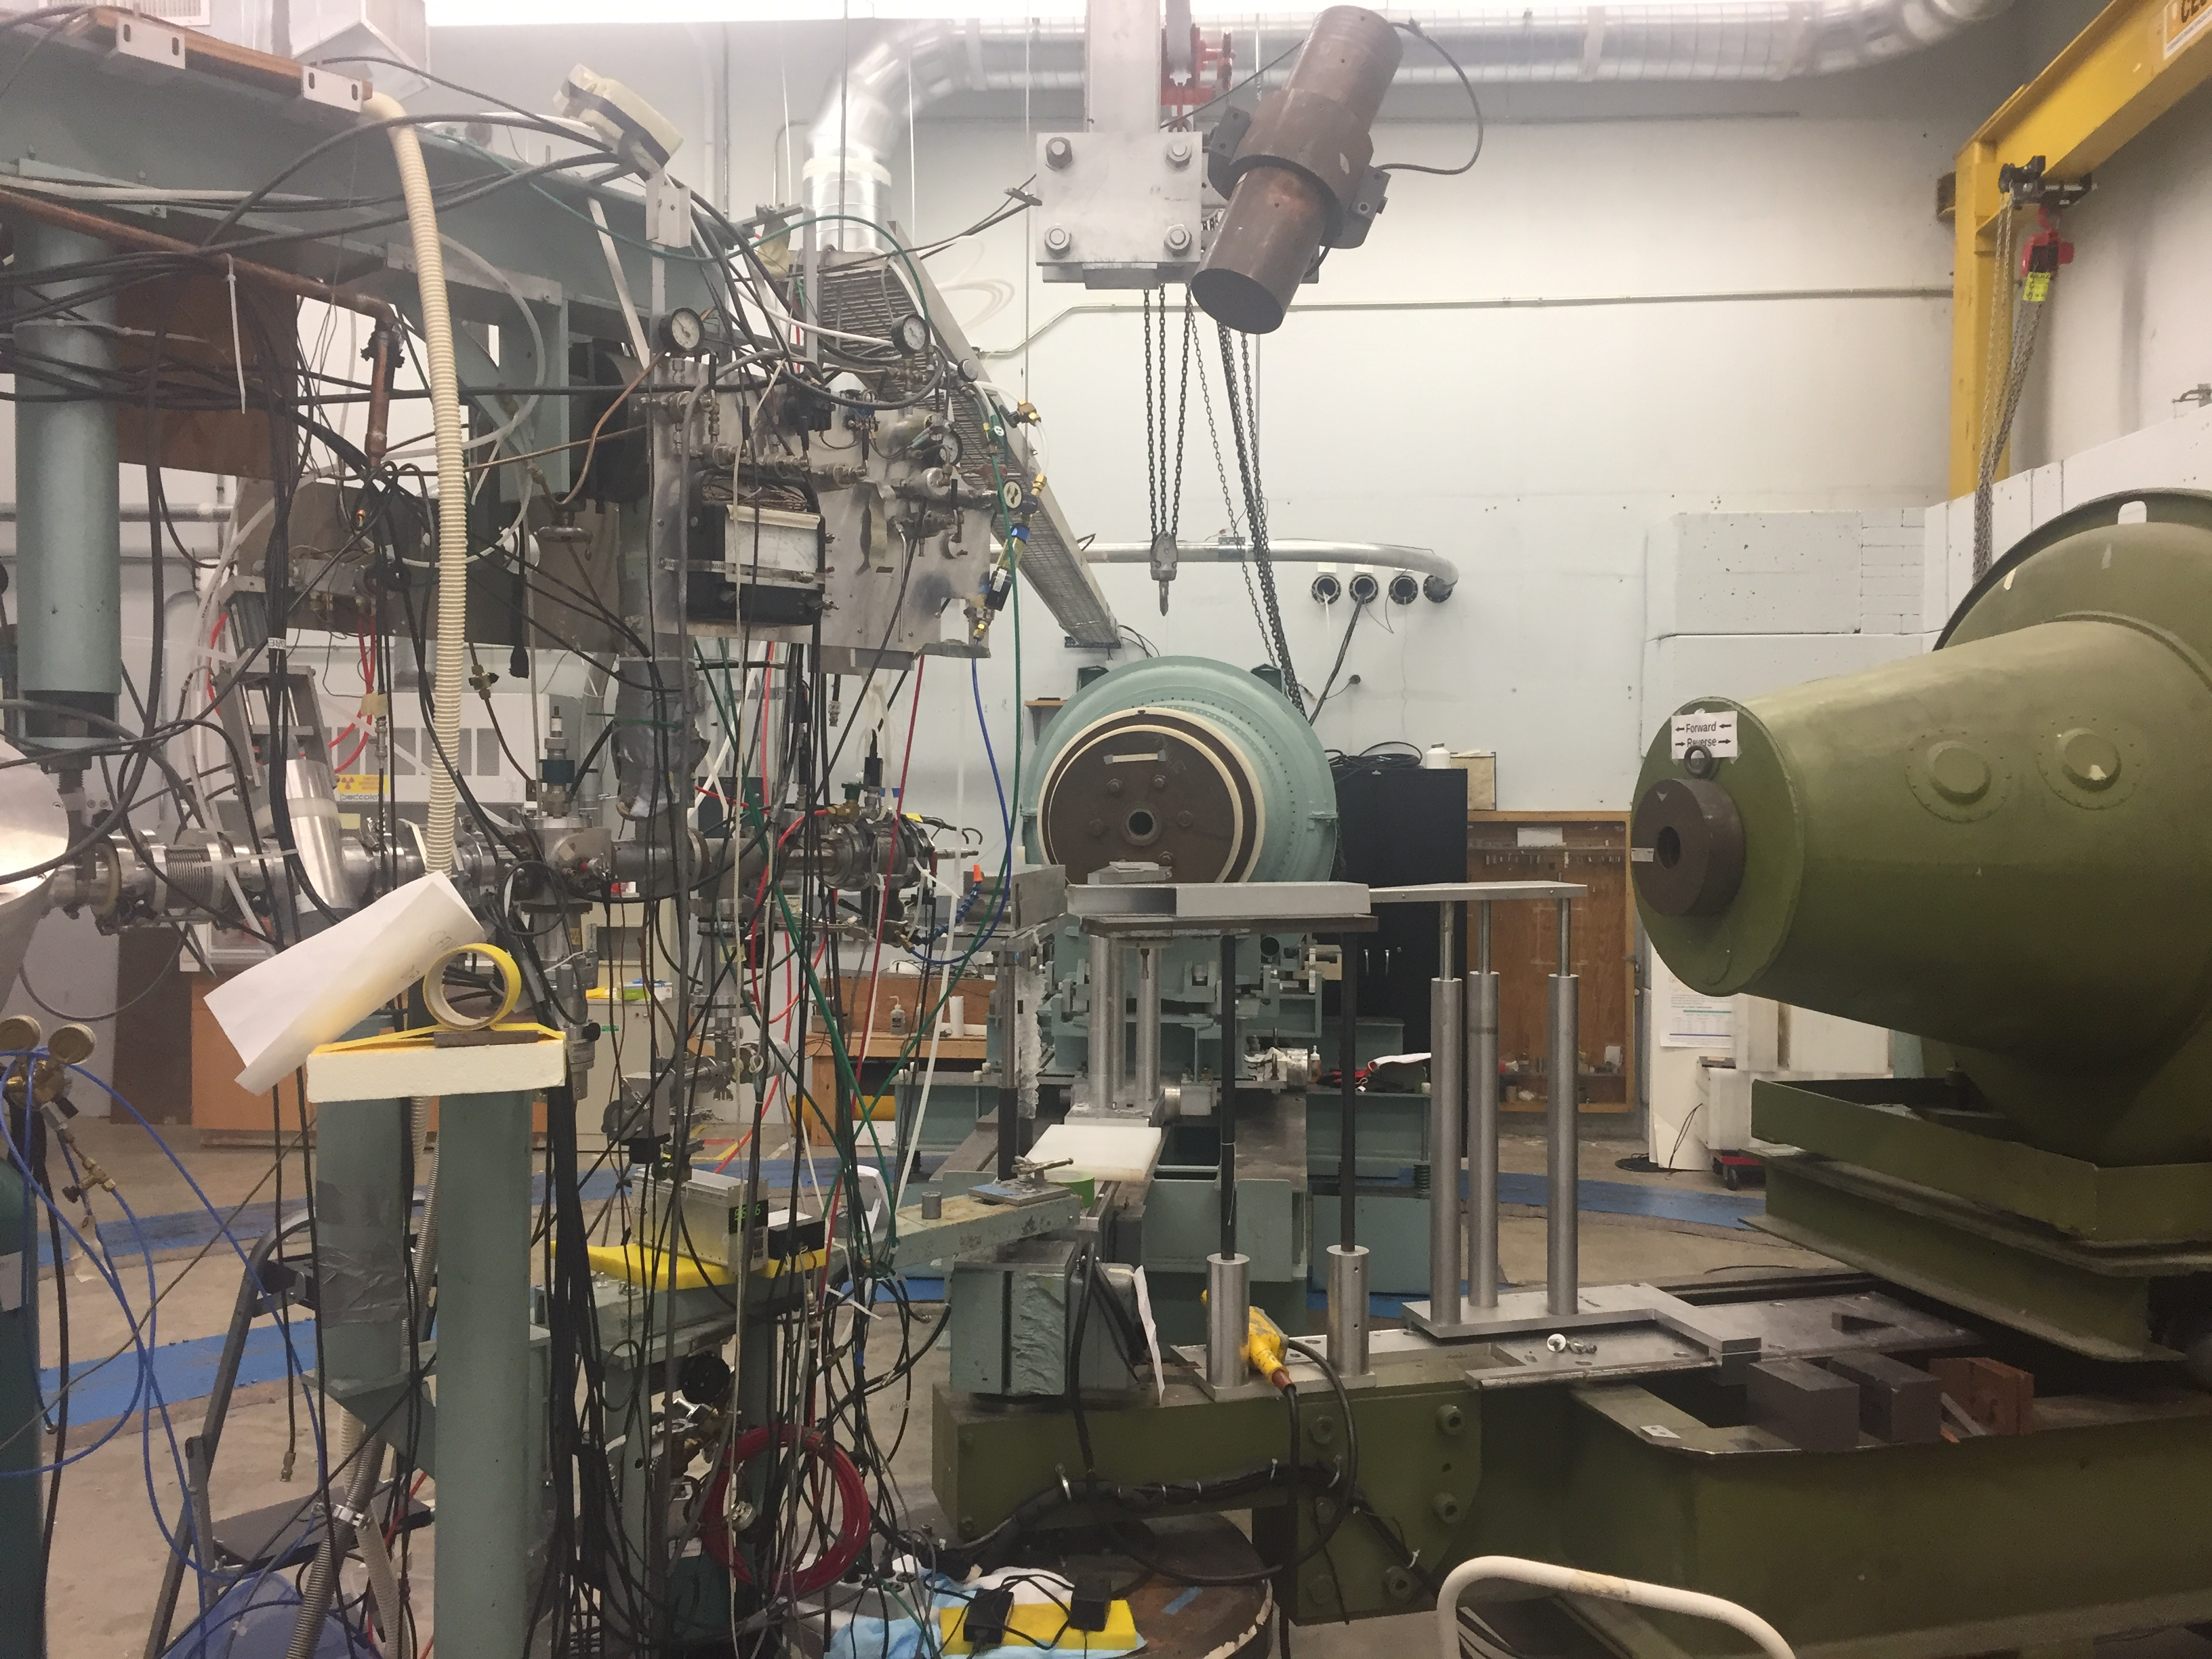
\includegraphics[width = 0.9\textwidth]{figures/TOFRoomPhoto.jpg}
    \caption[Image of the neutron TOF room at TUNL] 
    {
    Image of the neutron TOF room at TUNL. The deuteron beam pipe is visible on the left and
    terminates in a small deuteron gas target in the middle of the image, where neutrons are
    produced. The two detector arms are shown at center (6M) and right (4M). The ceiling
    monitor detector (CMON), which records beam flux, is visible at the top of the image.
    }
    \label{TOFRoomPhoto}
\end{figure}

\section{Data Acquisition}
Timing, pulse-shape discrimination, and pulse height information were
extracted by the analog signal processing logic laid out in Fig. \ref{ECSLogicDiagram}.
Raw signals from each neutron detector are processed by Mesytec MPD-4
pulse-shape-discrimination modules. The pulse tail length is converted to an
amplitude via a time-to-analog converter (TAC), providing neutron-gamma
discrimination. The pulse amplitude is measured by a separate
analog-to-digital converter (\gls{ADC}). Event times (labeled ``Gate'' from each MPD-4)
are passed as logic signals to a single time-to-digital converter (\gls{TDC}) so that
event times are recorded using a single clock. Pulse counts (``scalers'') are
collected at each step and the TDC, ADC, and data acquisition computer busy
signals are used to arrest the TDC when the system is already busy processing,
avoiding event pile-up.

\begin{sidewaysfigure}[tb]
    \centering
    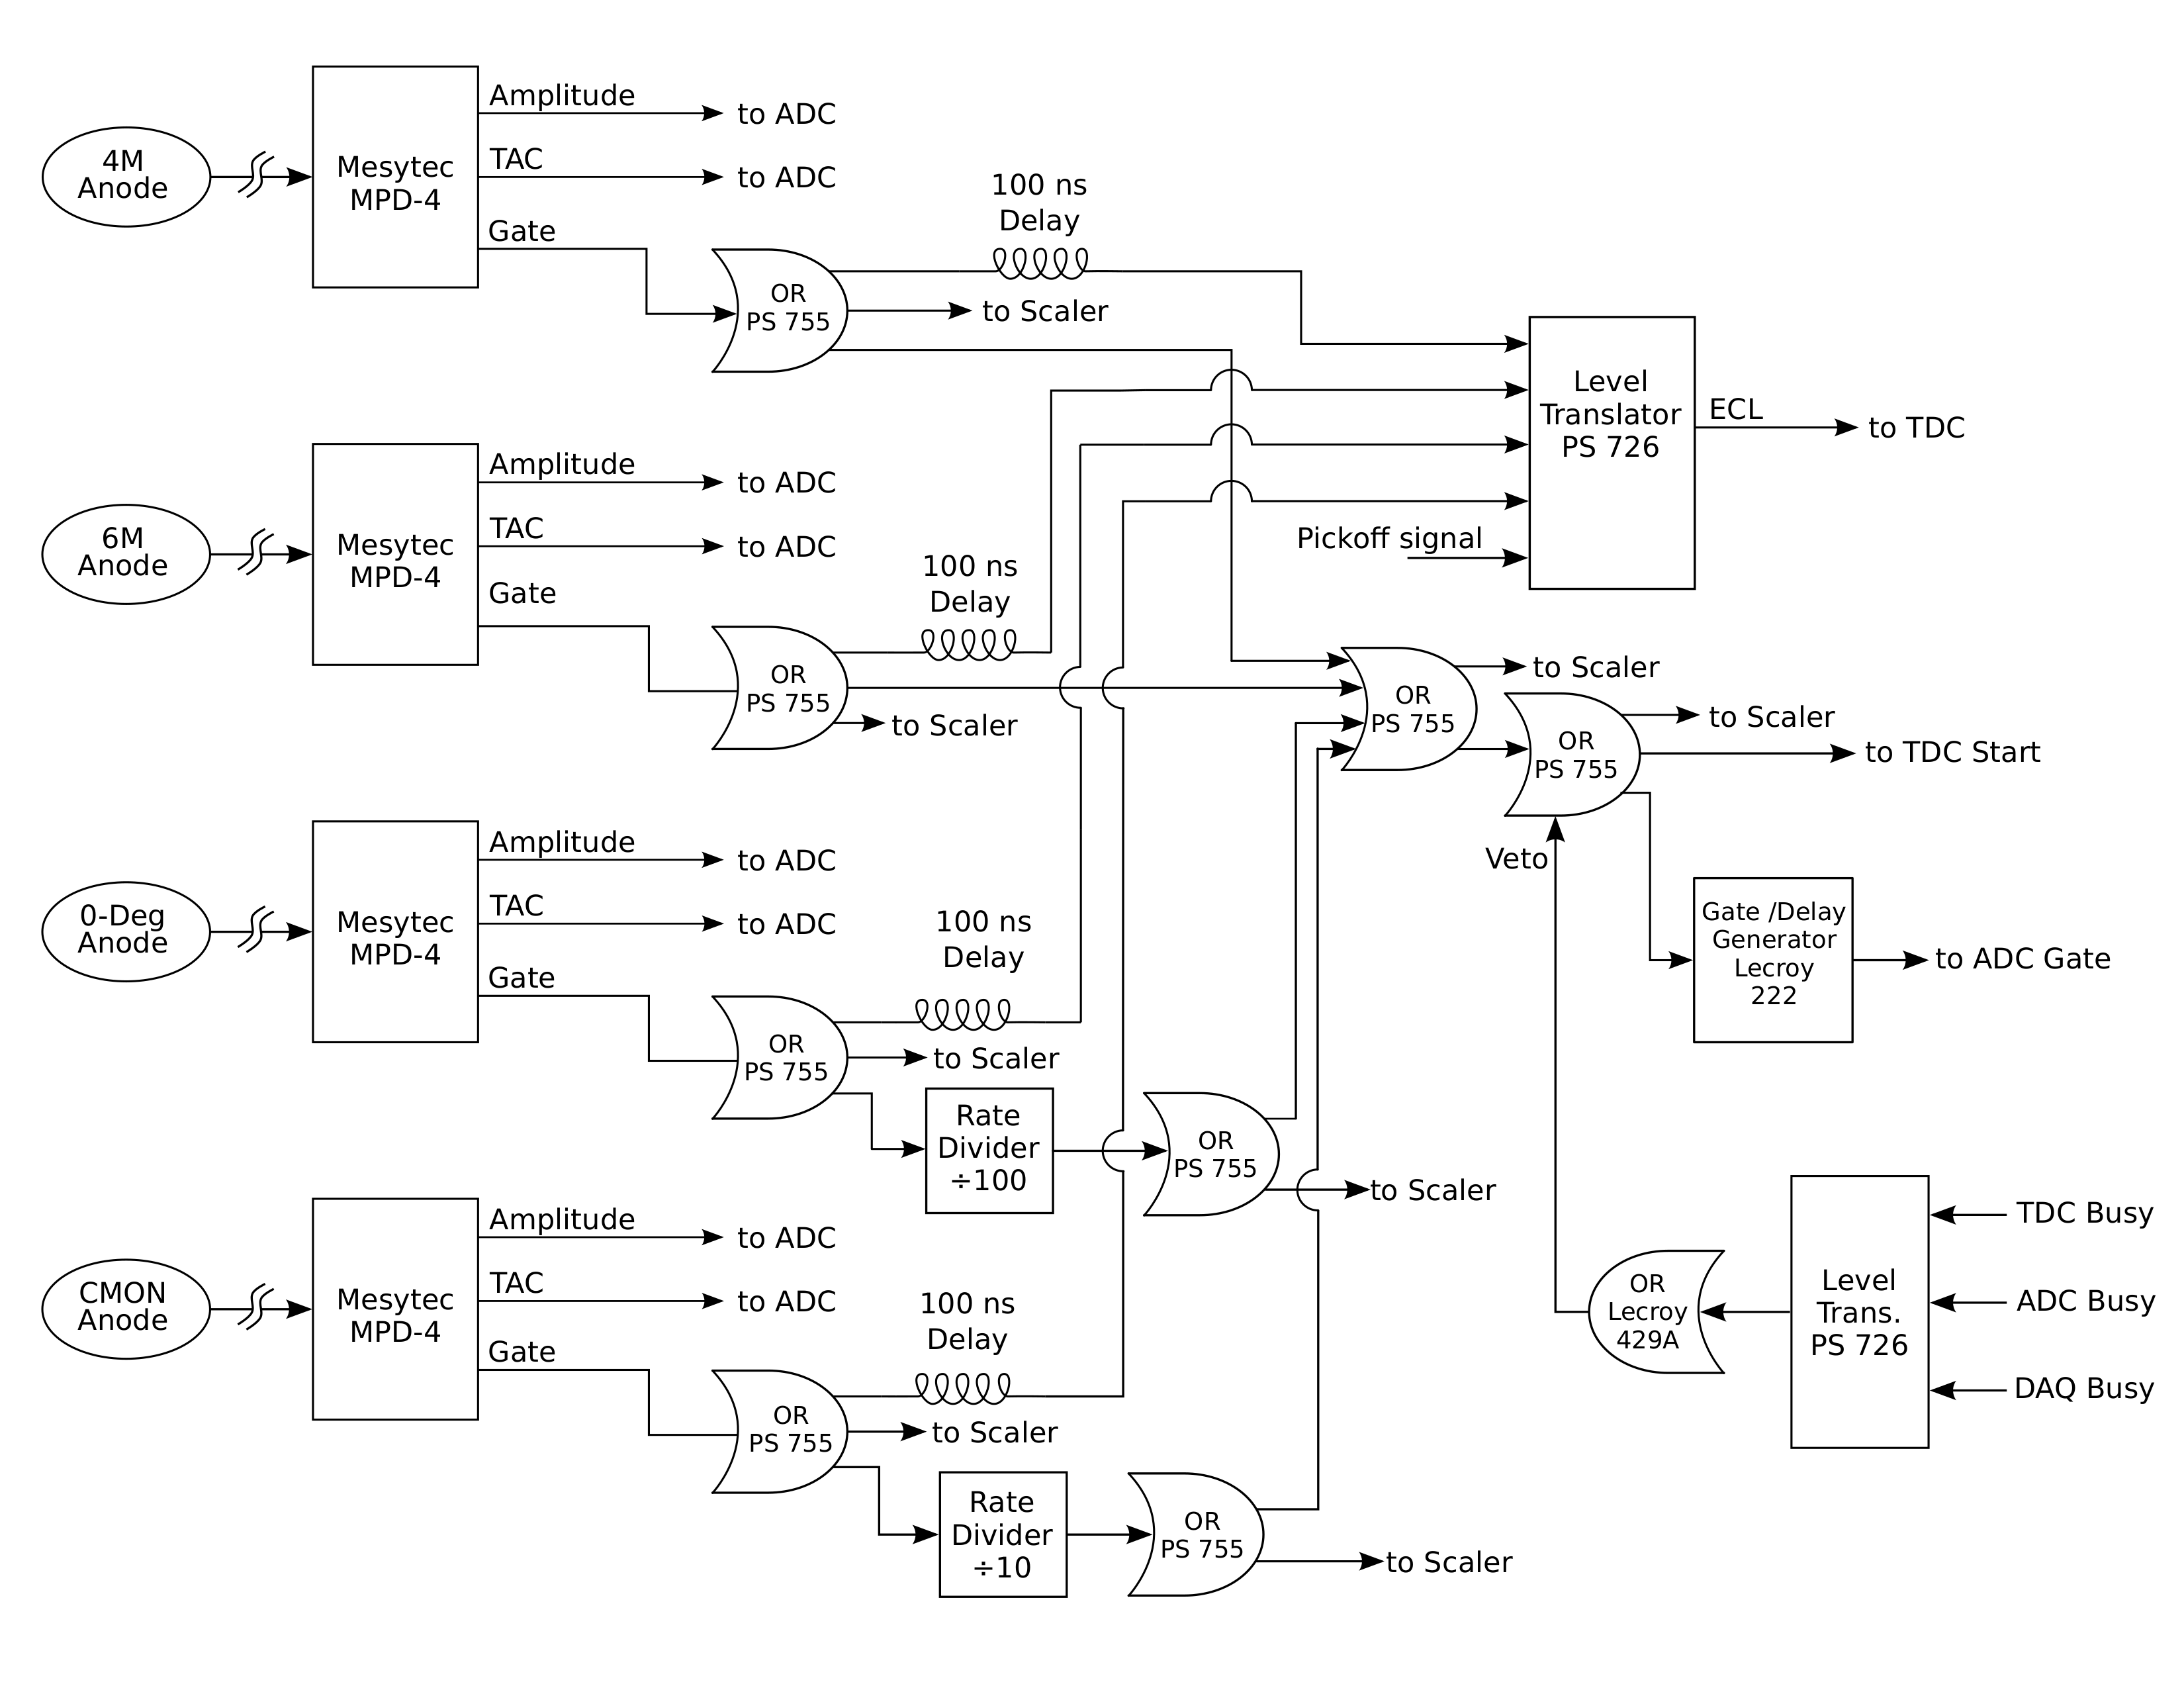
\includegraphics[width=0.9\textwidth]{figures/ECSLogic.png}
    \caption[Logic diagram for neutron \el\ data acquisition]
    {Logic diagram for neutron \el\ data acquisition at the TUNL time-of-flight
    room. Details are given in the text. Figure courtesy Ron Malone at TUNL.}
    \label{ECSLogicDiagram}
\end{sidewaysfigure}


\chapter{Neutron Elastic Cross Sections: Analysis and Results} \label{ECSAnalysis}
\section{Detector Characterization and Calibration}
Neutron energy was determined by time-of-flight, and neutron-gamma differentiation
determined by combining pulse shape discrimination (PSD) using [MODULE NAME] with
a gate on pulse height (PH). Neutron events were histogrammed by energy and the
number of counts in each bin was corrected for energy-dependent detector
efficiency [figure reference].

Initial runs were taken using (in series) a graphite, a polyethylene, and a blank
sample. A comparison of the spectra for these samples shows a peak for elastic
scattering on protons easily identifiable in the polyethylene spectrum but
absent in the graphite and blank spectra. Given the well-established n(p,p)n
cross section [cite reference] and the physical characteristics of the samples,
the ratio of incident neutron flux to the number of CMON counts can be calculated
(see [insert equation], [figure reference]). This flux-to-monitor ratio was used to normalize the
subsequent Sn sample measurements so absolute cross sections could be reported.

During data production, runs were taken in batches of three: one using 112Sn,
one using 124Sn, and one with a blank. For each angle of a given angular arm, the
efficiency-corrected histograms were normalized by the run's CMON counts,
and the relevant blank-run histogram subtracted from the isotopic-run
histograms. The major background contribution, visible in blank-run histograms
([INSERT FIGURE]), is from elastic scattering on atmospheric nitrogen
in the immediate vicinity of the sample. To calculate the cross section, the
Sn elastic peak must be integrated and the N elastic and Sn first-inelastic
peaks must be excluded. At forward angles and high neutron energies, the
difference in energy between Sn-elastic, Sn-inelastic, and N-elastic neutron
decreases and the separation between the peaks is reduced. Measurements in this
kinematic regime are the most challenging as the increased overlap between
these peaks increases the uncertainty in the Sn-elastic integral.

\begin{figure}
    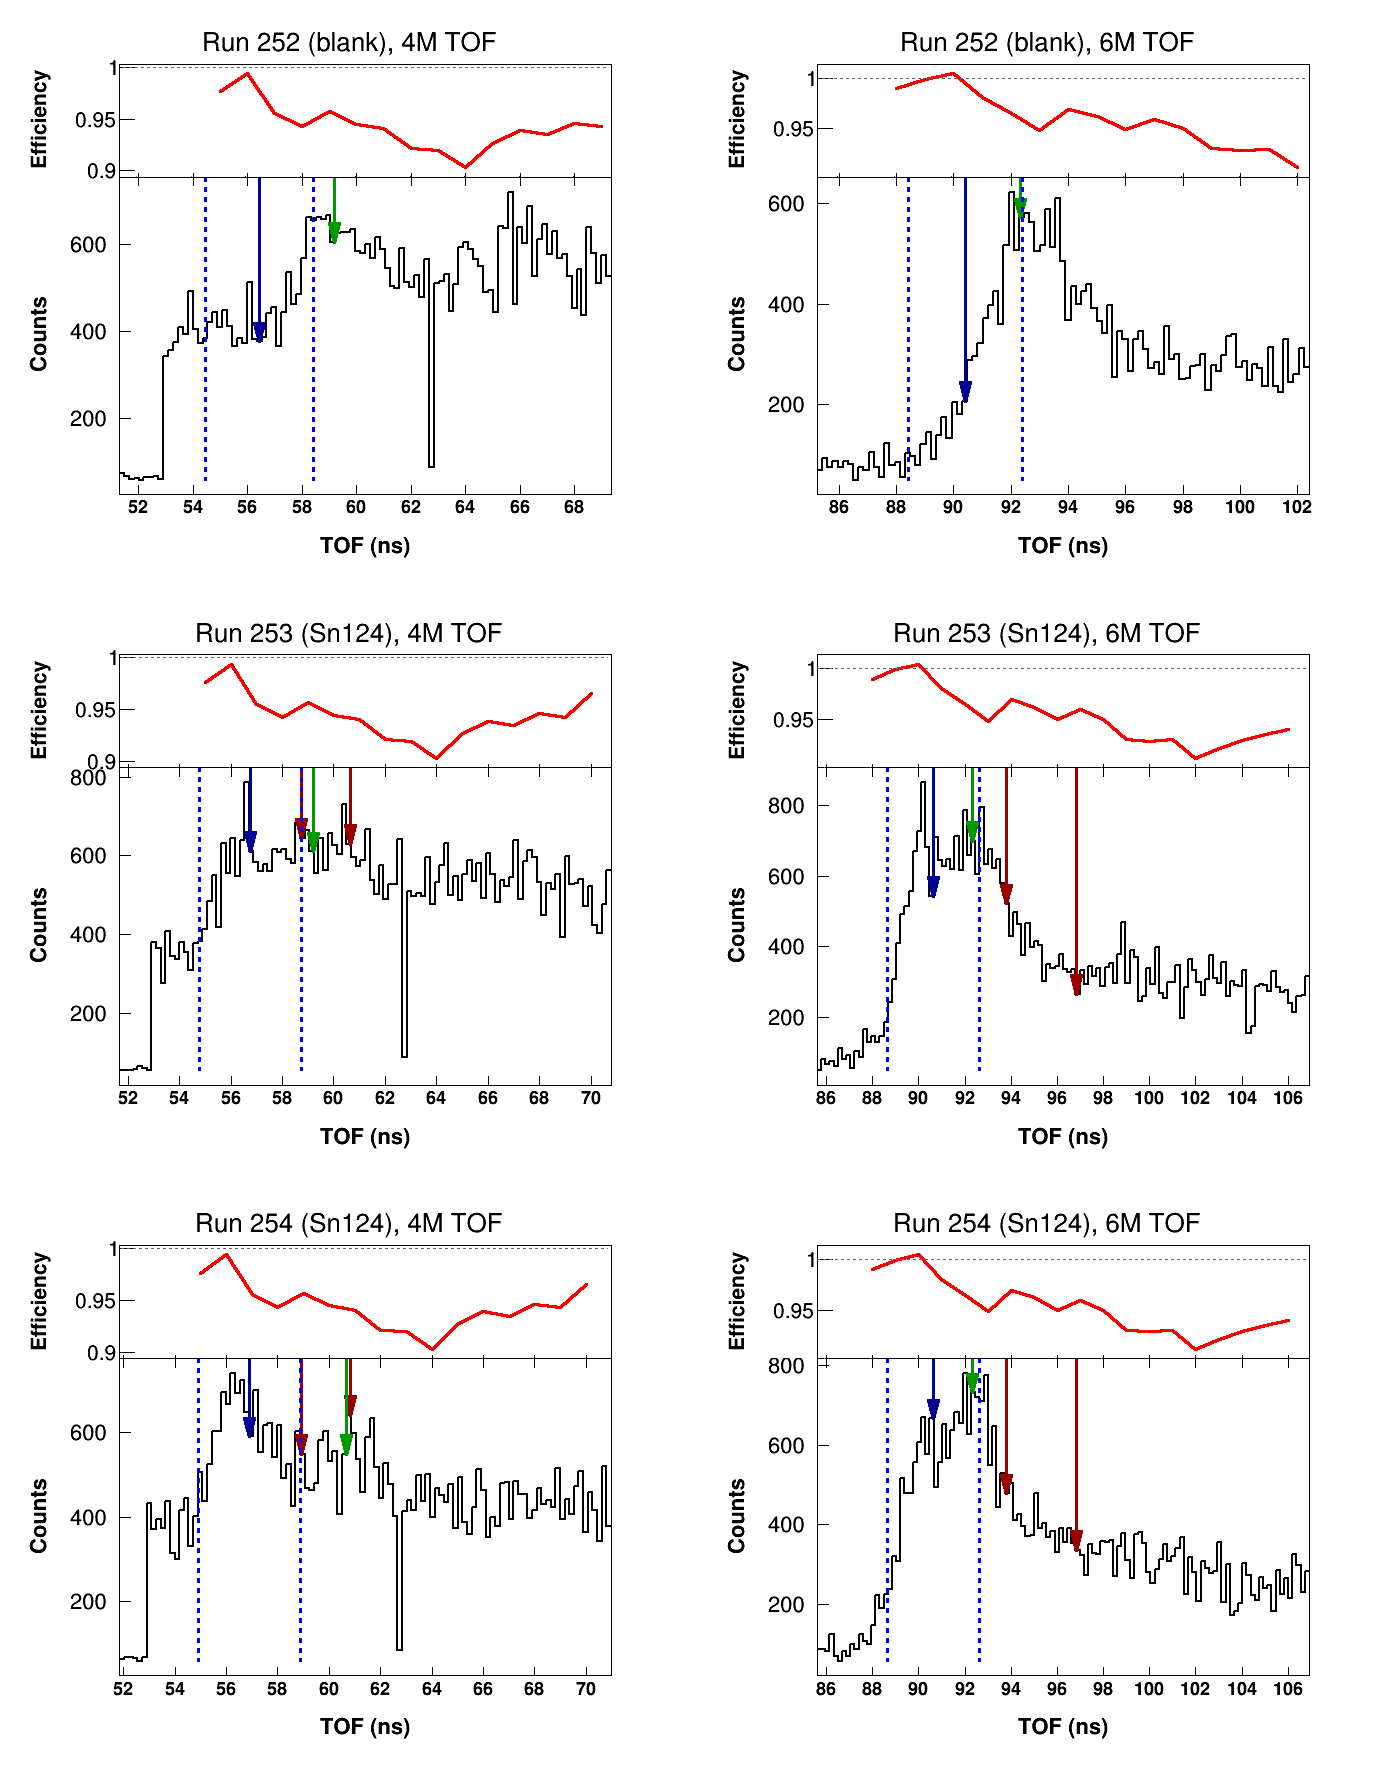
\includegraphics[width = 0.9\textwidth]{figures/tiledRunData.png}
    \caption{Typical raw event histograms showing neutron elastic scattering peak} \label{tiledRunData}
\end{figure}

Raw histograms of neutron events for several runs are shown. The
        expected location of the Sn elastic scattering peak (dark blue arrow)
        and first two inelastic scattering peaks (light blue arrows) show that
        only with the target in-beam (runs X, Y, Z) do the Sn elastic scattering
        peaks appear. For reference, the expected location of the nitrogen elastic scattering
    peak is shown in green.

\begin{figure}
    \includegraphics[width = 0.9\textwidth]{figures/tiledAngleData.png}
    \caption{Scaled event histograms showing neutron elastic scattering peak}
        \label{tiledAngleData}
\end{figure}

The background subtraction and integration procedure is shown for
        runs at 50 degrees. Sample-in-beam and sample-out-of-beam runs are
        separately summed (light gray histogram and dark gray histogram,
        respectively) and scaled by the number of monitor counts during those
        runs. The difference between those histograms (shown in red) shows a
        large elastic scattering peak at the expected TOF location (dark blue
        arrow); the first two inelastic scattering peaks (light blue arrows) are
        also shown. A double-Gaussian is fitted to the elastic and
        first-inelastic peaks and the first Gaussian integrated to recover the
        number of counts in the elastic peak. For reference, the expected location
        of the nitrogen elastic scattering peak is shown in green.

\begin{figure}
    \includegraphics[width = 0.9\textwidth]{figures/polyethyleneRef.png}
    \caption{Reference run histograms showing neutron scattering on C and (CH$_{2}$)$_{n}$}
    \label{polyethyleneRef}
\end{figure}

Histograms from an example polyethylene and a graphite run (light gray
histogram and dark gray histogram, respectively) used to normalize the
cross sections. Each histogram is scaled by the number of monitor counts during
that run and their difference is taken, yielding neutrons elastically scattered
from hydrogen (red histogram). The prominent neutron-hydrogen peak is
integrated between the gates (dashed lines) and combined with the
well-established n-p cross section to create a normalization factor for
the Sn runs. The neutron TOFs for scattering from carbon (elastically at the dark blue
arrow, to the first excited state of carbon at the light blue arrow)
and nitrogen (elastically at the green arrow) are indicated.

\begin{figure}[ht]
    \includegraphics[width=0.9\textwidth]{figures/PHPSDPlot.png}
    \caption{The pulse height (PH) versus pulse-shape-discrimination (PSD) for
    events of a typical run.}
    \label{PHPSDPlot}
\end{figure}

\section{Corrections and Gating}
Efficiency correction was straightforward: the detector response with respect to
neutron energy had already been tabulated by TUNL staff. Accordingly, we
adjusted the number of counts in each bin of our detector histograms according
to the bin's energy (shown in Fig. [X]). 

\subsection{Finite Size Correction}
Because the samples and angular detectors are not point-like, the exact
path of elastically-scattered neutrons is subject to a small degree of angular
uncertainty. The effect of this uncertainty is a "washing out" of measured cross
section maxima and minima with respect to the true cross section, especially in
regions where the cross section varies rapidly compared to the degree of
uncertainty. To assess the magnitude of this effect, a finite-size
simulation was prepared in which our measured cross section was assumed
to be the true cross section. In the simulation, a uniform beam of neutrons
impinged on the sample volume and was scattered into angular detectors where
hits were recorded. The resulting cross section [insert figure reference] is
thus a weighted convolution of the input cross section with the size uncertainty
of the samples and detectors. A comparison between the input and output cross
sections shows the finite-size effect is quite small in our case, much smaller
than statistical and other systematic errors. Still, to offset this effect, an
angle-dependent finite-size correction has been calculated and applied in all
results presented below.

In an idealized version of our differential cross
section measurement, the smaller the sample and neutron detectors are,
the more precisely
the angle of scattering of an incident neutron can be determined. Unfortunately,
smaller samples also reduce the rate of scattering and smaller detectors
reduce the solid angle in which scattered neutrons can be measured, both of
which reduce the number of detected neutrons and increase the statistical
uncertainty of the measurement. The experimentaler is thus responsible for applying
appropriate corrections so that reported results are apparatus-independent.

In the case of our differential cross section measurement at TUNL, the detectors'
composition, the geometry of the TOF room, and beam characteristics were
determined by the default configuration of the TUNL facility. Our samples were already
appropriately shaped for the TUNL TOF room sample suspension system and were
used for the measurement without modification. Given this configuration, we
identified two areas of concern requiring correction: the energy-dependence of
the detector efficiency ("efficiency correction") and the uncertainty in the
scattering angle due to the finite size of our sample and detectors ("finite
size correction").

To understand finite-size effects, a
Monte Carlo simulation was developed in which the sample and detector geometry
could be varied and the effect on the cross section visualized. As illustrated
in Fig. [X], in an experiment with point-like detectors and
samples, the scattering angle for a given configuration can be exactly
determined. In a realistic experiment, however, the finite size of the sample
introduces uncertainty in the location of the scattering vertex and the finite size of the
detector introduces uncertainty in the location of the detection vertex. Consequently, the cross
section calculated for a given angle also includes unwanted contributions
from nearby angles; correcting for this effect is essentially a "deconvolution"
of the scattering trajectories with respect to the sample and detector geometry.

For simplicity, the simulation was purely geometric - no nuclear physics or
energy-dependence was included. For each Monte Carlo iteration, the beam was
assumed to uniformly illuminate
the sample from one direction so that the scattering vertex was randomly
distributed within the sample volume. At the scattering vertex, a neutron
trajectory was selected by randomly sampling an "input cross section" as a
probability mass function, thus weighting the neutron scattering angles by the
input cross section.  Once the trajectory was known, each detector's location
and orientation was used to calculate the point of intersection in the plane of each detector. If the
intersection fell within the detector's face, the detector registered a hit.
Finally, the "output cross section" (that is, the result of the simulation)
was calculated by normalizing the number of counts registered in each detector
over the total number of iterations and the fraction of the total solid angle
subtended by said detector.

The results of the simulation are visible in Fig. [X]. For the sample and
detector sizes actually used in the experiment, the deviation between the input
and output cross sections is <1\% over all angles. When exaggerated sizes for the
sample and detectors are used, the finite-size effect is visible as a "washing
out" of minima and maxima in regions where the cross section varies rapidly with
angle. To calculate a correction factor for our results, we divided the simulation's
input cross section by the output cross section for each angle and multiplied our
experimental results by this factor. In principle, this procedure to generate
the correction should be repeated iteratively because the correction changes the input distribution 
used for the simulation itself, but in practice the correction is so small
that no further iteration is required.

\section{Cross Section Calculation}

\section{Results}
\subsection{\snTwelveFour\ \el\ at 11 MeV}
Absolute cross sections 

\begin{figure}
    \begin{center}
        \includegraphics[width = 0.9\textwidth]{figures/neutronECS_Sn_11MeV.png}
        \caption{Neutron \el cross sections on $^{112,124}$Sn at 11
    MeV: our results and literature data}
    \label{SnECS_11MeV}
\end{center}
\end{figure}

\subsection{\snTwelveFour\ \el\ at 17 MeV}

\begin{figure}
    \begin{center}
        \includegraphics[width = 0.9\textwidth]{figures/neutronECS_Sn_17MeV.png}
        \caption{Neutron \el cross sections on $^{112,nat,124}$Sn at 17
    MeV: our results and literature data} \label{SnECS_17MeV}
\end{center}
\end{figure}

\afterpage{\clearpage}


\chapter{Dispersive Optical Model Results}\label{DOMResults}
The \gls{DOM} fits on \oSixEight, \caAughtEight, \niEightFour,
\snTwelveFour, and \pbEight\ presented in
this chapter are the culmination of the new \tot\ and \el\ experimental results
(Chapters \ref{TCSAnalysis} and \ref{ECSAnalysis})
and new computational improvements in our DOM code (Chapter \ref{DOMFormalism}).
Previous DOM treatments have either used a
local equivalent potential \cite{Charity2006, Mueller2011} that was unsuitable for extracting
normalized bound-state wavefunctions or only provided results on one or
two nuclei \cite{Mahzoon2017, Atkinson2018}. All nine fits detailed here use the same fully-non-
local approach
(outlined in chapter \ref{DOMFormalism}) and lay the groundwork for a comprehensive DOM treatment 
across the chart of nuclides.

Beginning with \caForty, results from our new analyses of
\caAughtEight\ are compared to the previous
DOM analyses of \cite{MahzoonPhDThesis} and 
\cite{Atkinson2018}. Highlights from our results on \oSixEight, \niEightFour, \snTwelveFour,
and \pbEight\ are then presented; a complete picture of the fits on these nuclei
is reserved for Appendix \ref{DOMVisualization}. Last, general trends are identified across
all nine nuclei and successes and deficiencies of the present DOM treatment are pointed out.
A complete list of experimental data used to constrain the fits is provided in Appendix
\ref{DOMDataSets}. The best-fit parameter values for each nucleus are given in Appendix
\ref{DOMParameters}.

\section{Results for \caAughtEight}
As doubly-closed, mid-A nuclei, \caAughtEight\ are heavy enough for both density functional
theory (DFT) calculations \cite{Piekarewicz2012} and light enough for \textit{ab initio} 
treatments \cite{Hagen2016}. As such, they have long been cornerstone nuclei for
nuclear modeling. The size of the neutron skin of \caEight\ (along with that of $^{132}$Sn and
\pbEight) is of great theoretical interest as it is expected to be tightly correlated with the
density-dependence of the symmetry energy \cite{Fattoyev2012}. A model-independent determination
of the neutron skin thickness of \caEight\ is the goal of the upcoming parity-violating
electron scattering measurement CREX \cite{Horowitz2014}. Given this degree of interest in Ca
isotopes, optical models have been applied to
\caAughtEight\ more than almost any other nuclei. Thanks to the
great deal of high-quality \caAughtEight\ 
elastic and inelastic nucleon scattering data, quasi-free scattering data, and elastic electron
scattering data are available, \caAughtEight\ are ideal
candidates to test the DOM approach. To orient the
reader and facilitate a comparison to previous DOM treatments, the \caAughtEight\ fit results are
presented in greater detail than are the fit results on \oSixEight, \niEightFour,
\snTwelveFour, and \pbEight\ presented in later sections.

\subsection{Results for \caForty}
As with previous DOM treatments of \caForty\ \cite{MahzoonPhDThesis}, the present fit
quickly converged on proton and neutron elastic and inelastic scattering data from 10-200
\mega\electronvolt\ (shown in Figs. \ref{CaProtonElasticReproduced} and
\ref{CaNeutronElasticReproduced}). Because the \caForty\ proton \rxn\ 
has been
measured up to 200 \mega\electronvolt, the energy-dependence of the imaginary volume potential, 
$W_{vol}^{+}$, was well-constrained, expediting the fitting process
and lending confidence to the quality of our fit. Inelastic scattering data for
protons and neutrons on \caForty\ are shown in Figs. \ref{Ca40ProtonInelastic}
and \ref{Ca40NeutronInelastic}. 

Table \ref{Ca40ParticleNumber} shows the nucleon occupancy associated with each
set of quantum numbers $LJ$ as calculated from our \caForty\ fit. We see
slightly less depletion of the proton 1\sOne\ and 0\dThree\ occupancy than the
treatments of \cite{MahzoonPhDThesis, Mahzoon2017}, but there is qualitative
agreement. In both treatments, the correct total proton and neutron numbers were
achieved within 1\% of the real values. In Figure \ref{s1Depletion}, is clear
that without $\approx$30\%
depletion of the proton 0\sOne\ and 1\sOne\ shells, the charge density at the core of
\caForty\ would be too high,
a characteristic failure of mean-field models that do not account for depletion. 
The spectral functions of \caForty\ nucleons that 
we extract from the fit (Fig. \ref{Ca40SpectralFunctions})
show spectral peak broadening compared 
to the mean-field expectation, in keeping with (e,e'p) and (p,2p) measurements
\cite{Jacob1966, Jacob1973}.

\begin{table}[tb]
    \caption[\caForty\ proton and neutron occupancies from our DOM analysis]
    {
        \caForty\ proton and neutron occupancies by orbital angular momentum
        $L$ and total angular momentum $J$ from our DOM analysis. While
        most of the particle occupancy resides in states completely
        filled in an independent-particle-model (0\sOne, 0\pThree, 0\pOne, 0\dFive, 0\dThree,
        and 1\sOne\ for \caForty), 5-10\% of the occupancy appears in
        higher-angular-momentum states.
    }
    \centering
    \begin{tabular}{c c c c c c c c c c c}
        \toprule
        LJ & \sOne & \pThree & \pOne & \dFive & \dThree & \fSeven & \fFive &
        \gNine & \gSeven & Total\\
        \midrule
        $\pi_{occ}$ & & & & & & & & & & \\
        $\nu_{occ}$ & & & & & & & & & & \\
        \bottomrule
        \label{Ca40ParticleNumber}
    \end{tabular}
\end{table}

\begin{figure}[tb]
    \centering
    \includegraphics[width=0.85\textwidth]{figures/ca40_protonElastic.png}
    \caption[Proton elastic scattering cross sections on \caForty: DOM predictions and experimental data]
    {
        Proton elastic scattering cross sections on \caForty: experimental data
        and results from DOM fit. Experimental data are shown as points and
        calculated values from the DOM fit of these data are shown as lines.
        Differential cross sections (\el) are shown in the left panel and
        analyzing powers are shown in the right panel. For visual clarity, the 
        data have been offset along the ordinate axis so that the highest-energy data
        appear at the top of the figures. Data are colored according to the
        energy ranges shown in the left panel. References to all experimental data are listed
        in Appendix \ref{DOMDataSets}.
    }
    \label{CaProtonElasticReproduced}
\end{figure}
\begin{figure}[tb]
    \centering
    \includegraphics[width=0.85\textwidth]{figures/ca40_neutronElastic.png}
    \caption[Neutron elastic scattering cross sections on \caForty: DOM predictions and experimental data]
    {
        Neutron elastic scattering cross sections on \caForty: experimental data
        and results from DOM fit. Experimental data are shown as points and
        calculated values from the DOM fit of these data are shown as lines.
        Differential cross sections (\el) are shown in the left panel and
        analyzing powers are shown in the right panel. For visual clarity, the 
        data have been offset along the ordinate so that the highest-energy data
        appear at the top of the figures. Data are colored according to the
        energy ranges shown in the left panel. References to all experimental data are listed
        in Appendix \ref{DOMDataSets}.
    }
    \label{CaNeutronElasticReproduced}
\end{figure}

\begin{figure}[tb]
    \centering
    \begin{subfigure}[c]{\textwidth}
        \centering
        \includegraphics[width=0.82\textwidth]{figures/ca40_protonInelastic.png}
        \caption[Proton \rxn\ of \caForty: DOM predictions and experimental data]
        {
            Proton reaction cross sections on \caForty: experimental data and
            DOM predictions. Experimental data are shown as points and 
            calculated values from our DOM fit of these data are shown
            by the line. References to all experimental
            data are listed in Appendix \ref{DOMDataSets}.
        }
        \label{Ca40ProtonInelastic}
    \end{subfigure}\vspace{16pt}
    \begin{subfigure}[c]{\textwidth}
        \centering
        \includegraphics[width=0.82\textwidth]{figures/ca40_neutronInelastic.png}
        \caption[Neutron \rxn\ and \tot\ of \caForty: DOM predictions and experimental data]
        {
            Neutron reaction and total cross sections on \caForty: experimental data and
            DOM predictions. Experimental data are shown as points and 
            calculated values from our DOM fit of these data are shown
            by the line. References to all experimental
            data are listed in Appendix \ref{DOMDataSets}.
        }
        \label{Ca40NeutronInelastic}
    \end{subfigure}
\end{figure}

\begin{figure}[tb]
    \centering
    \includegraphics[width=\textwidth]{figures/ca40_SPLevels.png}
    \caption[Single-particle levels in \caForty]
    {
        Single-particle energy levels in \caForty\ for protons and neutrons.
        In each panel, calculated energies are shown on the left and
        experimental energies are shown on the right. References to all
        experimental data used to estimate these energy levels are
        listed in Appendix \ref{DOMDataSets}.
    }
    \label{Ca40SPLevels}
\end{figure}

\begin{figure}[tb]
    \centering
    \includegraphics[width=\textwidth]{figures/ca40_protonSpectralFunctions.png}
    \caption[Proton spectral functions in \caForty]
    {
        Proton spectral functions by orbital angular momentum $L$ and total
        angular momentum $J$ in \caForty, as generated by our DOM fit.
        In deeply-bound shells,
        spectral peak broadening is obvious, a consequence of increased
        imaginary strength in the self-energy at energies far from the
        Fermi energy. The shape and location of the \textit{neutron} spectral
        functions in \caForty\ are similar except for a Coulomb shift. The
        general shape and degree of occupation depletion associated with our spectral
        functions agree with results of (p,2p) and (e,e'p) scattering
        and former DOM treatments \cite{MahzoonPhDThesis}.
    }
    \label{Ca40SpectralFunctions}
\end{figure}

\begin{figure}[tb]
    \centering
    \begin{subfigure}[c]{\textwidth}
        \centering
        \includegraphics[width=0.75\textwidth]{figures/ca40_chargeDensity.png}
        \caption[Proton single-particle density distributions in \caForty]
        {
            Charge density distribution of \caForty, as generated
            by our DOM fit (in red) and as generated from experimental
            elastic electron scattering \cite{DeVries1987}. No error bars are
            reported in the compilated of \cite{DeVries1987}; we show an
            arbitrary uncertainty range of 1\% (blue shaded region).
        }
        \label{Ca40ChargeDensity}
    \end{subfigure}\vspace{16pt}
    \begin{subfigure}[c]{\textwidth}
        \centering
        \includegraphics[width=0.75\textwidth]{figures/ca40_protonLJDensityDist.png}
        \caption[Proton single-particle density distributions in \caForty]
        {
            Proton single-particle density distributions in \caForty, as generated
            by our DOM fit. Only the \sOne\ has density at the origin, which
            means that to recover the correct charge density at the origin, the
            occupation of the proton 0\sOne\ and 1\sOne\ in \caForty\ must be
            deplying by 20-30\%. That the bound LJs are significantly
            depleted indicates the importance of
            accounting for short- and long-range correlations when extracting
            structural information.
        }
        \label{s1Depletion}
    \end{subfigure}
\end{figure}

\begin{figure}[tb]
    \centering
    \begin{subfigure}[c]{\textwidth}
        \centering
        \includegraphics[width=0.75\textwidth]{figures/ca40_protonLJMomentumDistIntegral.png}
        \caption[Proton momentum distribution in \caForty]
        {
            Integrated proton momentum distribution in \caForty, as generated
            by our DOM fit. For the slightly-occupied proton \fSeven, \fFive, and
            \gNine\ and higher shells (which are completely vacant in an
            independent-particle model), a significant fraction of their
            density lies above 270 $\mega\electronvolt/\text{c}$ (indicated by
            the shaded gray region). The fraction of
            proton high-momentum content is slightly lower than that of neutrons
            (figure below), a consequence of Coulomb repulsion slightly reducing
            proton density in the core. The fraction of proton density with
            momentum above 270 $\mega\electronvolt/\text{c}$ is listed.
        }
        \label{Ca40ProtonMomentumDistInt}
    \end{subfigure}\vspace{16pt}
    \begin{subfigure}[c]{\textwidth}
        \centering
        \includegraphics[width=0.75\textwidth]{figures/ca40_neutronLJMomentumDistIntegral.png}
        \caption[Neutron momentum distributions in \caForty]
        {
            Integrated neutron momentum distribution in \caForty, as generated
            by our DOM fit. The slightly-occupied neutron \fSeven, \fFive, and
            \gNine\ shells make a significant contribution to the high-momentum
            content above 270 $\mega\electronvolt/\text{c}$ (indicated by the
            shaded gray region), as is true for the protons in the figure at top
            of the page. The fraction of neutron density with
            momentum above 270 $\mega\electronvolt/\text{c}$ is listed.
        }
        \label{Ca40NeutronMomentumDistInt}
    \end{subfigure}
\end{figure}

\begin{figure}[tb]
    \centering
    \includegraphics[width=\textwidth]{figures/ca40_protonVolumeIntegrals.png}
    \caption[Volume integral of proton imaginary potential in \caForty]
    {
        Volume integral of proton imaginary potential in \caForty. Above the
        Fermi energy, the surface-associated and volume-associated strength
        are clearly identifiable around 40 MeV and above 100 MeV,
        respectively. Near the Fermi energy, the potential is symmetric.
        Below the Fermi energy, the reduction of phase space reduces the
        magnitude of imaginary strength, but even at very negative energies,
        there is some strength. The small -- but signficant -- occupation at
        very negative energies make an outsized contribution to the total
        binding energy.
    }
    \label{Ca40ProtonVolumeIntegral}
\end{figure}

\begin{figure}[tb]
    \centering
    \includegraphics[width=\textwidth]{figures/ca40_matterDensity.png}
    \caption[Proton and neutron matter density distributions in \caForty]
    {
        Proton and neutron point density distributions in \caForty, as
        generated by our DOM fit. The RMS radii of the distributions and their
        difference (the neutron skin) are provided. In a symmetric system like
        \caForty, the neutron skin is expected to be slightly negative as a
        consequence of slight reduction of proton density in the core from
        Coulomb repulsion. The neutron skin we extract is in good agreement with
        the previous DOM fit of \cite{MahzoonPhDThesis}.
    }
    \label{Ca40MatterDistribution}
\end{figure}

\begin{figure}[tb]
    \centering
    \begin{subfigure}[c]{\textwidth}
        \centering
        \includegraphics[width=0.75\textwidth]{figures/ca40_EnergyDist.png}
        \caption[Energy density distribution for protons in \caForty]
        {
            Energy density distribution for protons in \caForty, as generated
            by our DOM fit. Valence nucleons (e.g., in the proton 1\sOne\ and
            0\dThree\ subshells in \caForty) contribute only slightly to the binding
            energy.
        }
        \label{Ca40EnergyDist}
    \end{subfigure}\vspace{16pt}
    \begin{subfigure}[c]{\textwidth}
        \centering
        \includegraphics[width=0.75\textwidth]{figures/ca40_EnergyDistIntegral.png}
        \caption[Total energy density integral in \caForty]
        {
            Total energy density integral in \caForty, as generated
            by our DOM fit. The total binding energy and binding energy per
            nucleon are given.
        }
        \label{Ca40EnergyDistIntegral}
    \end{subfigure}
\end{figure}

From the spectral functions, the momentum-space distribution for protons and neutrons was
calculated (shown in Figs. \ref{Ca40ProtonMomentumDistInt} and
\ref{Ca40NeutronMomentumDistInt}). The amount of ``high-
momentum content'' of these distributions is of great interest, as significant high-momentum content 
indicates deviation from the mean-field picture due to short-range correlations (SRCs). SRCs arise 
even in very light nuclear systems (e.g., \heFour)
and are associated with an altered quark distribution in nucleons 
\cite{Hen2012, Arrington2012, CLAS2019}.
Tensor-force interactions in neutron-proton pairs are thought to be a dominant source of 
SRCs \cite{Subedi2008}. Thus in symmetric nuclei like \cTwelve\ and \caForty, the
high-momentum content is expected to be nearly the same for protons and neutrons, whereas in
asymmetric nuclei like \pbEight, the minority nucleon species is expected to have a larger
high-momentum tail in the momentum distribution. In \cite{Rohe2004}, the \cTwelve\ proton and
neutron momentum distributions showed that $\approx$10\% of the nucleon density
has momentum above roughly 270 \mega\electronvolt\per{c}.
From our DOM fits, we calculate values of [insert ca40 momentum for p/insert ca40 momentum for n]\%
for protons and neutrons respectively, in line with the expectation that the high-momentum content
should increase slightly as one moves to higher A.

The total binding energy for \caForty\ is readily calculated using Eq.
\ref{TotalEnergyEquation}. Its radial dependence is shown in Fig.
\ref{Ca40EnergyDistIntegral} and the
contributions to the binding energy from each single-particle LJ are shown in
\ref{Ca40EnergyDist}. Per our fit, even though the 0\sOne\ nucleons consitute only [insert \%
of 0\sOne occupation] of the forty nucleons in \caForty, they provide a significant
share of the binding
energy ([insert binding energy \% for protons and neutrons]). At the spectral
functions (Fig. \ref{Ca40SpectralFunctions}) reveal, 0\sOne\ nucleons spend a small but significant portion of their time 
at very negative energies ($<$-100 \mega\electronvolt), pulling the weighted average binding energy 
closer to 8.5 \mega\electronvolt\per{A}, the experimental binding energy for \caForty. In this
picture, it is clear why mean-field models consistently underpredict the binding energy, as they
cannot adequately represent the nucleon-nucleon correlations associated with the long
negative-energy tail of the spectral functions.

Lastly, from the proton and neutron point distributions generated by our fit, we calculate a
\caForty\ neutron skin for of [insert neutron skin] fermi (see Fig. \ref{Ca40MatterDistribution}). 
This is in good agreement with the skin calculated in previous DOM treatments
\cite{MahzoonPhDThesis} and with the expectation that the neutron skin should be slightly negative in
symmetric nuclei, a consequence of Coulomb repulsion nudging proton density toward the surface.

\subsection{Results for \caEight}
The recent non-local DOM treatment of Mahzoon et al. \cite{Mahzoon2017} was able
to reproduce a wide variety of
experimental data on \caEight\ and recovered a \caEight\ neutron
skin of 0.249 $\pm$ 0.023 \femto\meter.
This neutron skin value is significantly higher than the 0.132 \femto\meter calculated by
the \textit{ab initio} treatment of \cite{Hagen2016}. Mahzoon et al. found that when the 
smaller \textit{ab initio} was forcibly applied to their fit, it disturbed the fit's
reproduction of experimental \caEight\ neutron \tot\ data, implying that the neutron \tot\ might
be sensitive to the neutron skin thickness. In this work, our fit on \caEight\ uses essentially the 
same experimental data used by Mahzoon et al. but less than half as many potential parameters.
By comparing results, we glean some insight about the uniqueness of each DOM fit and what parameters
are most closely connected to the neutron skin thickness.

[insert \caEight\ matter density distributions]

\section{Results for \oSixEight}
The lightest system analyzed in the DOM framework, \oSix\ is a valuable benchmark
for $\chi$-EFT, shell model, and ab initio approaches. A wealth of scattering and
bound-state information have been collected on \oSix, making it a good test case for the validity
of the DOM in light systems and helping to validate the choices of DOM potential forms.

Of the nuclides we chose for a DOM treatment, \oEight\ was one of most challenging due to the 
paucity of
available experimental data, the lightness of the system, and the neutron open shell.
To constrain the negative-energy domain
of the potential, the only available experimental data were the neutron and proton separation
energies and the RMS charge radius of \oEight\ and \neEight, making fitting easier but adding to the
uncertainty in the \oEight\ negative energy parameterization.

\subsection{Results for \oSix}
The large corpus of experimental data used to constrain the \oSix\
potential includes proton \el\ and analyzing powers up to 200 MeV, neutron \el\ and analyzing powers
up to 100 MeV, proton \rxn\ cross section up to 65 MeV, and qualitative knowledge about the shape of
the spectral functions of the bound $\pi$ \sOne, \pThree, and \pOne\ subshells from (e,e'p)
measurements. Good agreement with all 
experimental data was achieved, excepting the highest-energy ($>$ 150 \mega\electronvolt)
proton differential elastic cross sections and analyzing powers, especially at backward angles.

For a system as light as \oSix, the density of states at low energies (i.e., below the neutron
separation energy) is sufficiently low that a smoothly-varying potential will be a poor
approximation of the resonance structure that dictates the strength of inelastic scattering. This
deficiency is particularly acute in the doubly-closed-shell nuclei, where the level spacing is
larger near the Fermi energy. We expect this to be a contributing factor to the slight
overestimation of the RMS charge radius (see Fig. \ref{o16ChargeDensity}).

\begin{figure}[tb]
    \centering
    \begin{subfigure}[c]{\textwidth}
        \centering
        \includegraphics[width=0.75\textwidth]{figures/o16_chargeDensity.png}
        \caption[Proton single-particle density distributions in \oSix]
        {
            Charge density distribution of \oSix, as generated
            by our DOM fit (in red) and as generated from experimental
            elastic electron scattering \cite{DeVries1987}. No error bars are
            reported in the compilated of \cite{DeVries1987}; we show an
            arbitrary uncertainty range of 1\% (blue shaded region).
        }
        \label{o16ChargeDensity}
    \end{subfigure}\vspace{16pt}
    \begin{subfigure}[c]{\textwidth}
        \centering
        \includegraphics[width=0.75\textwidth]{figures/o16_protonLJDensityDist.png}
        \caption[Proton single-particle density distributions in \oSix]
        {
            Proton single-particle density distributions in \oSix, as generated
            by our DOM fit.
        }
        \label{o16LJDensityDist}
    \end{subfigure}
\end{figure}

As with \caForty\ and \pbEight, (e,e'p) cross sections have been measured on \oSix. These data
provide direct access to the momentum distribution of bound nucleons and are thus a critical test
for the validity of our fits. Figure \ref{O16eep} presents the results of a calculation of (e,e'p)
cross sections from the DWEEPY code \cite{Atkinson2018, Giusti2011} that uses the DOM potential and partial waves as input.
It is important to note that these data were not used in the fitting of the DOM
potential for \oSix\ and thus they give an indication of how well
the DOM potential can be used for prediction rather than just reproduction of experimental data.

\begin{figure}[tb]
    \centering
    \includegraphics[width=0.9\textwidth]{figures/O16eep.png}
    \caption[\oSix\ (e,e'p) cross sections calculated by the DOM]
    {
        \oSix\ (e,e'p) cross sections calculated by the DOM (solid line) and experimental data from
        \cite{Leuschner1994}.
    }
    \label{O16eep}
\end{figure}

As with \caForty, we see that \oSix\ has a slightly negative neutron skin: [insert o16 neutron skin]
\femto\meter\ as extracted from our optimized fit.

\subsection{Results for \oEight}
No experimental \oEight\ charge density distribution was available, so we generated
an approximate charge density distribution for \oEight\ by linearly scaling
the radii and densities of the \oSix\ charge density distribution to reproduce the \oEight\ RMS charge
radius and maintain a total charge of 8. The reported RMS charge radii of \oSix\ and \oEight\ differ by only
0.01 fm (<0.5\%), so the approximate \oEight\ charge density distribution we generated is barely
distinguishable from the \oSix\ distribution. This same scaling procedure was also employed to
generate a charge density distribution for \snTwelve, using the
experimentally-derived \snFour\ charge density distribution. To initiate the fit, the \oSix\ best-fit parameter values
were assigned to the \oEight\ parameter file and calculated observables were generated to compare
with \oEight\ data. The \oSix\ optimized parameter values were moderately successful at reproducing
the \oEight\ scattering data without further adjustment, though almost no neutron scattering data is
available besides our newly-measured \tot. Using the raw \oSix\ parameters, the DOM predictions for
\oEight\ proton SP levels were underbound by several \mega\electronvolt\
and the calculated particle number was too low, unsurprising
given the insufficiency of the \oSix\ Hartree-Fock term to account for 
two additional nucleons' worth of binding in \oEight. Thus, before
loosening any other parameters, the HF depth and HF depth asymmetry terms were allowed to vary,
reducing the chi-square contribution from the charge density, particle number, and energy level
sectors. Once a chi-square minimum had been reached with these two parameters, all other 
parameters were allowed to vary. Our optimum fit achieved good agreement with all
experimental \oEight\ scattering data except the 24 MeV neutron elastic scattering data
of Grabmayr et al. \cite{Grabmayr1980}, where the DOM somewhat underestimates
the differential cross section throughout its range.

Figure \ref{o18MatterDensity} shows the matter density distributions for protons
and neutrons extracted from our fit on \oEight. We recover a large neutron skin of
0.197 \femto\meter, commensurate with the neutron skin of much more asymmetric
nuclei (cf. [insert pb neutron skin] of \pbEight). The reason is clear: most
of density from the two extra neutrons in \oEight\ goes into the
$\nu$0\dFive, which peaks at the nuclear surface, increasing the neutron RMS
radius. To test our extracted neutron skin thickness for \oEight\, we considered 
the difference in RMS charge radii between mirror nuclei \neEight\ and \oEight.
The values of 2.97 \femto\meter\ for \neEight\ from \cite{Marinova2011} and
2.79 \femto\meter\ for \oEight\ from \cite{DeVries} yield a difference of 0.18
\femto\meter, quite close to our extracted neutron skin for \oEight.

\section{Results for \niEightFour}
Unlike \caAughtEight, both \niEight\ and \niFour\ have partially-occupied neutron shells in the
independent-particle-model picture. Accordingly, Ni isotopes have increased level density near the
Fermi level and should possess significant imaginary strength in this region, impacting
low-energy elastic and inelastic nucleon cross sections. Recently, A. Brown has outlined a
program to constrain the density dependence of the symmetry energy using RMS charge radii in mirror
nuclei in the Fe and Ni region, heightening interest in accurate
matter density distributions for these isotopes.
\subsection{Results for \niEight}
Like \caForty, \niEight\ has enjoyed attention from experimentalists for many decades yielding
an abundance of proton and neutron elastic scattering data.
\subsection{Results for \niFour}
Due to its low natural abundance, \niFour\ is a dramatically more expensive target material than
\niEight\, limiting the coverage of experimental data for this isotope.

\section{Results for \snTwelveFour}
Of the isotopic systems studed in this treatment, \snTwelveFour\ was the least well-characterized by
experimental data. Our new neutron \tot\ and \el\ measurements provide a sizable fraction
of available nucleon scattering data on \snTwelveFour\ from 1-200 \mega\electronvolt. Due to the
lack of data, the Sn DOM fits presented here are the least well-constrained of all the fits
presented with the possible exception of \niFour. Still, the structural information exctracted from
our fits on \snTwelveFour\ largely comports with the trends seen in the other isotopic systems and
may be useful for extrapolating properties of the doubly-magic $^{100}$Sn and $^{132}$Sn. As
mid-shell nuclei, the Sn isotopes exhibit deformation and help provide important information
about deviations from the shell model outside shell closures. 
\subsection{Results for \snTwelve}
\subsection{Results for \snFour}

\section{Results for \pbEight}
The size of the neutron skin of \pbEight\ has been identified by numerous studies as highly
correlated with the density-dependence of the symmetry energy, $L$, a critical input for the neutron
star equation-of-state. By employing parity-violating electron scattering to probe the
weak charge distribution in \pbEight, the PREX experiment at Jefferson Laboratory extracted a
\pbEight\ neutron skin value of 0.33$\pm$0.17 fm. A followup experiment with improved statistics, PREX II,
is slated to run later in 2019, and is expected to constrain the \pbEight\ neutron skin thickness to
within 0.06 fm. Given the wide range of \pbEight\ neutron skin thicknesses predicted by relativistic
and non-relativistic mean-field models, an accurate calculation of this quantity is an excellent
test for the validity of the DOM treatment.

\begin{figure}[tb]
    \centering
    \begin{subfigure}[c]{\textwidth}
        \centering
        \includegraphics[width=0.75\textwidth]{figures/pb208_protonLJMomentumDistIntegral.png}
        \caption[Proton momentum distribution in \pbEight]
        {
            Integrated proton momentum distribution in \pbEight, as generated
            by our DOM fit. The fraction of proton high-momentum content is
            slightly higher than that of neutrons
            (figure below), a consequence of the enhancement in short-range
            corerlations (SRCs) experienced by the minority nucleon in an
            asymmetric system. The fraction of proton density with
            momentum above 270 $\mega\electronvolt/\text{c}$ is listed.
        }
        \label{pb208ProtonMomentumDistInt}
    \end{subfigure}\vspace{16pt}
    \begin{subfigure}[c]{\textwidth}
        \centering
        \includegraphics[width=0.75\textwidth]{figures/pb208_neutronLJMomentumDistIntegral.png}
        \caption[Neutron momentum distributions in \pbEight]
        {
            Integrated neutron momentum distribution in \pbEight, as generated
            by our DOM fit. The fraction of neutron density with
            momentum above 270 $\mega\electronvolt/\text{c}$ is listed.
        }
        \label{pb208NeutronMomentumDistInt}
    \end{subfigure}
    \label{pb208Momenta}
\end{figure}

\begin{figure}[tb]
    \centering
    \includegraphics[width=\textwidth]{figures/pb208_matterDensity.png}
    \caption[Proton and neutron matter density distributions in \pbEight]
    {
        Proton and neutron point density distributions in \pbEight, as
        generated by our DOM fit. The RMS radii of the distributions and their
        difference (the neutron skin) are provided. The neutron skin of
        neutron-rich systems like \pbEight are expected to be strongly correlated
        with the size of the density-dependence of the symmetry energy, $L$.
    }
    \label{Pb208MatterDistribution}
\end{figure}

\section{General trends}
\subsection{Neutron skins sensitive to shell structure}
Table \ref{NeutronSkins} presents the neutron skins we extracted from our
optimized DOM fits on all nuclei under study. As anticipated both the total
degree of asymmetry and the specific shell structure affect the
calculated skins.
\begin{table}[H]
    \centering
    \begin{tabular}{c c c c}
        \toprule
        Isotope & proton $r_{rms}$ & neutron $r_{rms}$ & $\Delta_{rms}$\\
        \midrule
        \oSix & & & \\
        \oEight & & & \\

        \caForty & & & \\
        \caEight & & & \\

        \niEight & & & \\
        \niFour & & & \\

        \snTwelve & & & \\
        \snFour & & & \\

        \pbEight & & & \\
        \bottomrule
        \label{NeutronSkins}
    \end{tabular}
    \caption[Neutron skins extracted from DOM analysis]
    {
        Neutron skins ($\Delta_{rms})$) extracted from DOM analysis. The skins are calculated as the difference between the
        proton and neutron point distribution root-mean-square (RMS) radii and thus do not include the
        nucleon-size form factor. The full calculated matter distributions for protons and
        neutrons for each nucleus are available in Appendix \ref{DOMVisualization}. 
    }
\end{table}

\subsection{High-momentum content and deep imaginary strength}
When examined in momentum space, the proton and neutron particle density distributions
are expected to show significant enhancement of nucleon density at higher momentum
than would be expected in an independent-particle shell model
\cite{RoheHabilitation}. The amount of this so-called
"high-momentum content" has been investigated by knockout reactions
\cite{Rohe2004, RoheHabilitation} and shown to be significant even for very
light nuclei such as \cTwelve ($\approx10\% >
270 \mega\electronvolt/\text{c}$). Table \ref{HighMomentumContent} shows the
percentage of the proton and neutron densities above $270
\mega\electronvolt/\text{c}$ extracted from our DOM fits.
\begin{table}[tb]
    \caption[High-momentum content extracted from DOM analysis]
    {
        High-momentum content as extracted from DOM analysis. For protons and neutrons for each
        nucleus under study, the nucleon density distribution in momentum-space is calculated and
        the fraction of the density distribution above 270 \mega\electronvolt/c is
        tabulated. For comparison, \cite{Rohe2004} reported $\approx10\%$ high momentum content for
        \cTwelve. The full momentum-space matter distributions for protons and
        neutrons for each nucleus are available in Appendix \ref{DOMVisualization}. 
    }
    \label{HighMomentumContent}
    \centering
    \begin{tabular}{c c c c}
        \toprule
        Isotope & proton $p_{>270}$ & neutron $p_{>270}$ & p/n Ratio\\
        \midrule
        \oSix & & & \\
        \oEight & & & \\

        \caForty & & & \\
        \caEight & & & \\

        \niEight & & & \\
        \niFour & & & \\

        \snTwelve & & & \\
        \snFour & & & \\

        \pbEight & & & \\
        \bottomrule
    \end{tabular}
\end{table}
Our results comport with the expectation that heavier nuclei should have a
higher fraction of high-momentum nucleons, a consequence of their deeper central
potentials. Because the particle density of the nuclear core saturates around
0.16 $\femto\meter^{-3}$, it is sensible that the
high-momentum content fraction would grow only slowly with increasing A once
the core has reached this nucleon density (around \cTwelve-\oSix).
For the symmetric nuclei \oSix\ and \caForty, it is expected that the proton
high-momentum content should be slightly less than the neutron high-momentum
content due to a slight reduction in proton particle density at the nuclear
core, and that this effect should increase with increasing Z. For highly asymmetric
nuclei (e.g., \snFour, \pbEight), it is expected that the \textit{minority
nucleon species} should have a \textit{larger fraction of high-momentum
content} \cite{Subedi2008, Hen2012}, a consequence of the enhanced
short-range correlations for these nucleons. All of these expectations are borne
out in the momentum distributions we extract, bolstering confidence in the
quality of our fits.

It should be noted that the high-momentum tail of the
momentum-space distributions are very sensitive to the imaginary
strength at very deep energies. This is perfectly sensible, as the most deeply-bound
nucleons should have the highest-momentum. This deep
negative-energy realm is perhaps the least well-characterized part of our fit,
as our only direct constraint is the experimental binding energy. Because the
binding energy does not differentiate between protons and neutrons, we have
very limited sensitivity to the isovector-dependence of the potential in
this area. As a result, the relative high-momentum content between protons and
neutrons that we extract should only be taken qualitatively, though the absolute
high-momentum content values from our fits agree well with results from
\cite{Rohe2004, RoheHabilitation}.

\subsection{Overestimation of RMS charge radius}
All of the charge density distributions extracted from our fits showed a slight
excess of charge density on the extreme tail of the distributions (e.g., above 5 
\femto\meter\ for \caForty). As the RMS charge radius is most sensitive to
contributions from the tail, this excess led to chronic overestimation of the RMS
charge radius of 0.05-0.10 \femto\meter\ across nuclei.
We found that density in the extreme tail of the matter distributions was very
sensitive to the amount of imaginary strength just below the Fermi energy
($W_{sur}^{-}$); in fits with a high weight for the RMS charge radius,
$W_{sur}^{-}$ would tend toward zero or even cross into negative territory, an
unphysical result. Especially in the lighter systems we studied, our fits routinely
moved all the negative-energy imaginary strength into $W_{vol}^{-}$.
We had no difficulties fitting $W_{sur}^{+}$, largely due to the
availability of proton \rxn\ and neutron \tot\ data from 20-50 MeV.
Interestingly, the volume
integral of the imaginary strength (an integration over the
radial form factors) of our optimized fits shows the imaginary potential to be largely symmetric
about the Fermi energy within roughly 30 MeV (see Fig. \ref{Ca40ProtonVolumeIntegral}),
in keeping with the expectations of \cite{Mahaux1991} and many other theoretical
treatments. Whether the partitioning
of the negative-energy imaginary strength into $W_{vol}^{-}$ over $W_{sur}^{-}$
has real significance is unclear, but it suggests that subsequent 
analyses may need more specialized treatment in the negative-energy regime.

Practically speaking, because the nuclear surface and volume overlap
in light systems like \oSix, there is no unique best-fit for the
negative-energy parameters. In addition, in real nuclei near the Fermi surface,
imaginary strength should vary rapidly due to the discrete resonance structure of
the nucleus. In this region, the optical potential corresponds quite poorly
with reality as it can only represent a smooth average. With these
considerations in mind, it is perhaps
not surprising that we had trouble getting
the negative-energy surface parameters under control. In the end, for the light systems
discussed here (\oSixEight, \caAughtEight), we fixed $W_{sur}^{-}$ to zero for
the final optimizations to avoid numerical problems and prevent any
unphysical imaginary strength from arising. In our fits, the
$W_{vol}^{-}$ term had no trouble providing imaginary strength where it was
needed to recover correct particle numbers, charge density distributions, and,
to some extent, binding energies.

It should be noted that while we produce RMS charge radii that are a tad high
compared to experimental measurements, we had good success recovering the shape
of the full charge density distribution profiles. As the neutron skin is the
\textit{difference} between proton and neutron matter radii, any systematic
issues that affect both the neutron and proton matter distributions should not
affect our neutron skin values.
\afterpage{\clearpage}


\chapter{Conclusion}
\section{Implications of experimental \tot\ and \el\ results}
We have presented a new program of isotopic \tot\ measurements that provide critical data for
constraining the isovector strength of the nuclear potential at positive energies. By using
digitizer technology to reduce the processing time associated with each detection event by a factor
of ten, we were able to accumulate sufficient statistics far more quickly than in previous
measurements that used analog signal processing. Consequently, we were able to measure the \tot\ on
several rare isotopes up to 450 \mega\electronvolt, an energy range that was previously inaccessible.

\section{Implications of DOM results for nuclear structure}
- expect that while positive-energy scattering data can be well-approximated by
optical potentials even in nuclei lighter than \oSix, bound-state data is poorly
represented. Clustering and reduced level density make a smooth optical
potential a poor approximation. Heavy nuclei have sufficient phase space on both
sides of the Fermi energy that the nuclear potential can be reasonably
symmetric.

\section{Topics for Future Study}
\tot\ on Fe and Cd isotopes (cf. with Ni and Sn isotope studies), \tot\ on all stable Sn isotopes
Proton \rxn\ studies on O, Ni, and Sn isotopes
Covariance analysis of DOM parameters
Publication of the DOM codebase
Isotope chain calculations (\snTwelve\ to \snFour), as was done with local DOM
Extension to odd-even and odd-odd nuclei
Extraction of global optical model (cf. Koning-Delaroche)


\clearpage %needed this or for some reason the header writes appendix for the last chapter...

\fancyhead{} %clears the header
\fancyhead[LE]{\MakeUppercase{ \leftmark}} %rewrite fancy header to just label chapter name

\clearpage
\addcontentsline{toc}{chapter}{Bibliography}

\singlespacing
\bibliographystyle{unsrt}
\bibliography{references}
\doublespacing

\clearpage

\begin{appendices}

  %Reformat chapter titles so that they say appendix in the appendices
    \titleformat
    {\chapter} % command
    [display] % shape
    {\bfseries \Large} % format
    {Appendix \ \thechapter} % label %Here is where I write appendix, also \ moves you a space or two
    {0.1 in} % sep
    {
        \rule{\textwidth}{1pt}
        \vspace{0.2in}
    % \centering
        \raggedleft
    } % before-code
    [
        \vspace{-0.3in}%
        \rule{\textwidth}{1pt}
    ] % after-code
    \titlespacing*{\chapter}{0pt}{-22pt}{0pt}

    \fancyhead{} %clears the header
    \fancyhead[RO]{\MakeUppercase{appendix \thechapter \ \leftmark}} %rewrite fancy header to say appendix
    \chapter{DOM Fit Results}
    \label{DOMFits}

\section{DOM fit of \oSix}

\label{O16DOMOutput}
\begin{figure}[H]
    \centering
    \begin{minipage}{0.45\textwidth}
        \centering
        \includegraphics[width=1.0\textwidth]{figures/o16_protonElastic.png}
        \caption{\oSix\ proton elastic scattering data}
        \label{DOMFitData_o16_proton_elastic}
    \end{minipage}\hfill
    \begin{minipage}{0.45\textwidth}
        \centering
        \includegraphics[width=1.0\textwidth]{figures/o16_neutronElastic.png}
        \caption{\oSix\ neutron elastic scattering data}
        \label{DOMFitData_o16_neutron_elastic}
    \end{minipage}
\end{figure}

\begin{figure}[H]
    \centering
    \begin{minipage}{0.45\textwidth}
        \centering
        \includegraphics[width=1.0\textwidth]{figures/o16_protonInelastic.png}
        \caption{\oSix\ proton \rxn data}
        \label{DOMFitData_o16_proton_inelastic}
    \end{minipage}\hfill
    \begin{minipage}{0.45\textwidth}
        \centering
        \includegraphics[width=1.0\textwidth]{figures/o16_neutronInelastic.png}
        \caption{\oSix\ neutron \rxn and \tot data}
        \label{DOMFitData_o16_neutron_inelastic}
    \end{minipage}
\end{figure}

\afterpage{\clearpage}

\begin{figure}[H]
    \centering
    \begin{minipage}{0.45\textwidth}
        \centering
        \includegraphics[width=1.0\textwidth]{figures/o16_chargeDensity.png}
        \caption{\oSix\ charge density data}
        \label{DOMFitData_o16_chargeDensity}
    \end{minipage}\hfill
    \begin{minipage}{0.45\textwidth}
        \centering
        \includegraphics[width=1.0\textwidth]{figures/o16_SPLevels.png}
        \caption{\oSix\ single-particle levels}
        \label{DOMFitData_o16_SPLevels}
    \end{minipage}
\end{figure}

\afterpage{\clearpage}

\begin{figure}[H]
    \centering
    \begin{minipage}{0.45\textwidth}
        \centering
        \includegraphics[width=1.0\textwidth]{figures/o16_protonPotentials.png}
        \caption{\oSix\ proton potential energy-dependence}
        \label{DOMFitData_o16_proton_potentialComponent_energy}
    \end{minipage}\hfill
    \begin{minipage}{0.45\textwidth}
        \centering
        \includegraphics[width=1.0\textwidth]{figures/o16_neutronPotentials.png}
        \caption{\oSix\ neutron potential energy-dependence}
        \label{DOMFitData_o16_neutron_potentialComponent_energy}
    \end{minipage}
\end{figure}

\begin{figure}[H]
    \centering
    \begin{minipage}{0.45\textwidth}
        \centering
        \includegraphics[width=1.0\textwidth]{figures/o16_protonVolumeIntegrals.png}
        \caption{\oSix\ proton potential, integrated over r-space}
        \label{DOMFitData_o16_proton_potentialIntegral}
    \end{minipage}\hfill
    \begin{minipage}{0.45\textwidth}
        \centering
        \includegraphics[width=1.0\textwidth]{figures/o16_neutronVolumeIntegrals.png}
        \caption{\oSix\ neutron potential, integrated over r-space}
        \label{DOMFitData_o16_neutron_potentialIntegral}
    \end{minipage}
\end{figure}

\afterpage{\clearpage}

\begin{figure}[H]
    \centering
    \begin{minipage}{0.45\textwidth}
        \centering
        \includegraphics[width=1.0\textwidth]{figures/o16_protonSpectralFunctions.png}
        \caption{\oSix\ proton spectral functions}
        \label{DOMFitData_o16_proton_spectralFunctions}
    \end{minipage}\hfill
    \begin{minipage}{0.45\textwidth}
        \centering
        \includegraphics[width=1.0\textwidth]{figures/o16_neutronSpectralFunctions.png}
        \caption{\oSix\ neutron spectral functions}
        \label{DOMFitData_o16_neutron_spectralFunctions}
    \end{minipage}
\end{figure}

\begin{figure}[H]
    \centering
    \includegraphics[width = 0.5\textwidth]{figures/o16_matterDensity.png}
    \caption{\oSix\ matter density distribution}
    \label{DOMFitData_o16_matterDensity}
\end{figure}

\begin{figure}[H]
    \centering
    \includegraphics[width = 0.5\textwidth]{figures/o16_momentumDistribution.png}
    \caption{\oSix\ momentum distribution}
    \label{DOMFitData_o16_momentumDistribution}
\end{figure}

\begin{figure}[H]
    \centering
    \includegraphics[width = 0.5\textwidth]{figures/o16_energyDensity.png}
    \caption{\oSix\ energy density distribution}
    \label{DOMFitData_o16_energyDensity}
\end{figure}

\begin{figure}[H]
    \centering
    \includegraphics[width = 1.0\textwidth]{figures/o16_eep.png}
    \caption{\oSix\ (e,e'p) cross sections}
    \label{DOMFitData_o16_eep}
\end{figure}

\section{DOM fit of \oEight}
\label{o18DOMOutput}
\begin{figure}[H]
    \centering
    \begin{minipage}{0.45\textwidth}
        \centering
        \includegraphics[width=1.0\textwidth]{figures/o18_protonElastic.png}
        \caption{\oEight\ proton elastic scattering data}
        \label{DOMFitData_o18_proton_elastic}
    \end{minipage}\hfill
    \begin{minipage}{0.45\textwidth}
        \centering
        \includegraphics[width=1.0\textwidth]{figures/o18_neutronElastic.png}
        \caption{\oEight\ neutron elastic scattering data}
        \label{DOMFitData_o18_neutron_elastic}
    \end{minipage}
\end{figure}

\begin{figure}[H]
    \centering
    \begin{minipage}{0.45\textwidth}
        \centering
        \includegraphics[width=1.0\textwidth]{figures/o18_protonInelastic.png}
        \caption{\oEight\ proton \rxn data}
        \label{DOMFitData_o18_proton_inelastic}
    \end{minipage}\hfill
    \begin{minipage}{0.45\textwidth}
        \centering
        \includegraphics[width=1.0\textwidth]{figures/o18_neutronInelastic.png}
        \caption{\oEight\ neutron \rxn and \tot data}
        \label{DOMFitData_o18_neutron_inelastic}
    \end{minipage}
\end{figure}

\afterpage{\clearpage}

\begin{figure}[H]
    \centering
    \begin{minipage}{0.45\textwidth}
        \centering
        \includegraphics[width=1.0\textwidth]{figures/o18_chargeDensity.png}
        \caption{\oEight\ charge density data}
        \label{DOMFitData_o18_chargeDensity}
    \end{minipage}\hfill
    \begin{minipage}{0.45\textwidth}
        \centering
        \includegraphics[width=1.0\textwidth]{figures/o18_SPLevels.png}
        \caption{\oEight\ single-particle levels}
        \label{DOMFitData_o18_SPLevels}
    \end{minipage}
\end{figure}

\afterpage{\clearpage}

\begin{figure}[H]
    \centering
    \begin{minipage}{0.45\textwidth}
        \centering
        \includegraphics[width=1.0\textwidth]{figures/o18_protonPotentials.png}
        \caption{\oEight\ proton potential energy-dependence}
        \label{DOMFitData_o18_proton_potentialComponent_energy}
    \end{minipage}\hfill
    \begin{minipage}{0.45\textwidth}
        \centering
        \includegraphics[width=1.0\textwidth]{figures/o18_neutronPotentials.png}
        \caption{\oEight\ neutron potential energy-dependence}
        \label{DOMFitData_o18_neutron_potentialComponent_energy}
    \end{minipage}
\end{figure}

\begin{figure}[H]
    \centering
    \begin{minipage}{0.45\textwidth}
        \centering
        \includegraphics[width=1.0\textwidth]{figures/o18_protonVolumeIntegrals.png}
        \caption{\oEight\ proton potential, integrated over r-space}
        \label{DOMFitData_o18_proton_potentialIntegral}
    \end{minipage}\hfill
    \begin{minipage}{0.45\textwidth}
        \centering
        \includegraphics[width=1.0\textwidth]{figures/o18_neutronVolumeIntegrals.png}
        \caption{\oEight\ neutron potential, integrated over r-space}
        \label{DOMFitData_o18_neutron_potentialIntegral}
    \end{minipage}
\end{figure}

\afterpage{\clearpage}

\begin{figure}[H]
    \centering
    \begin{minipage}{0.45\textwidth}
        \centering
        \includegraphics[width=1.0\textwidth]{figures/o18_protonSpectralFunctions.png}
        \caption{\oEight\ proton spectral functions}
        \label{DOMFitData_o18_proton_spectralFunctions}
    \end{minipage}\hfill
    \begin{minipage}{0.45\textwidth}
        \centering
        \includegraphics[width=1.0\textwidth]{figures/o18_neutronSpectralFunctions.png}
        \caption{\oEight\ neutron spectral functions}
        \label{DOMFitData_o18_neutron_spectralFunctions}
    \end{minipage}
\end{figure}

\begin{figure}[H]
    \centering
    \includegraphics[width = 0.5\textwidth]{figures/o18_matterDensity.png}
    \caption{\oEight\ matter density distribution}
    \label{DOMFitData_o18_matterDensity}
\end{figure}

\begin{figure}[H]
    \centering
    \includegraphics[width = 0.5\textwidth]{figures/o18_momentumDistribution.png}
    \caption{\oEight\ momentum distribution}
    \label{DOMFitData_o18_momentumDistribution}
\end{figure}

\begin{figure}[H]
    \centering
    \includegraphics[width = 0.5\textwidth]{figures/o18_energyDensity.png}
    \caption{\oEight energy density distribution}
    \label{DOMFitData_o18_energyDensity}
\end{figure}

\section{DOM fit of \caForty}

\label{ca40DOMOutput}
\begin{figure}[H]
    \centering
    \begin{minipage}{0.45\textwidth}
        \centering
        \includegraphics[width=1.0\textwidth]{figures/ca40_protonElastic.png}
        \caption{\caForty\ proton elastic scattering data}
        \label{DOMFitData_ca40_proton_elastic}
    \end{minipage}\hfill
    \begin{minipage}{0.45\textwidth}
        \centering
        \includegraphics[width=1.0\textwidth]{figures/ca40_neutronElastic.png}
        \caption{\caForty\ neutron elastic scattering data}
        \label{DOMFitData_ca40_neutron_elastic}
    \end{minipage}
\end{figure}

\begin{figure}[H]
    \centering
    \begin{minipage}{0.45\textwidth}
        \centering
        \includegraphics[width=1.0\textwidth]{figures/ca40_protonInelastic.png}
        \caption{\caForty\ proton \rxn data}
        \label{DOMFitData_ca40_proton_inelastic}
    \end{minipage}\hfill
    \begin{minipage}{0.45\textwidth}
        \centering
        \includegraphics[width=1.0\textwidth]{figures/ca40_neutronInelastic.png}
        \caption{\caForty\ neutron \rxn and \tot data}
        \label{DOMFitData_ca40_neutron_inelastic}
    \end{minipage}
\end{figure}

\afterpage{\clearpage}

\begin{figure}[H]
    \centering
    \begin{minipage}{0.45\textwidth}
        \centering
        \includegraphics[width=1.0\textwidth]{figures/ca40_chargeDensity.png}
        \caption{\caForty\ charge density data}
        \label{DOMFitData_ca40_chargeDensity}
    \end{minipage}\hfill
    \begin{minipage}{0.45\textwidth}
        \centering
        \includegraphics[width=1.0\textwidth]{figures/ca40_SPLevels.png}
        \caption{\caForty\ single-particle levels}
        \label{DOMFitData_ca40_SPLevels}
    \end{minipage}
\end{figure}

\afterpage{\clearpage}

\begin{figure}[H]
    \centering
    \begin{minipage}{0.45\textwidth}
        \centering
        \includegraphics[width=1.0\textwidth]{figures/ca40_protonPotentials.png}
        \caption{\caForty\ proton potential energy-dependence}
        \label{DOMFitData_ca40_proton_potentialComponent_energy}
    \end{minipage}\hfill
    \begin{minipage}{0.45\textwidth}
        \centering
        \includegraphics[width=1.0\textwidth]{figures/ca40_neutronPotentials.png}
        \caption{\caForty\ proton potential energy-dependence}
        \label{DOMFitData_ca40_neutron_potentialComponent_energy}
    \end{minipage}
\end{figure}

\begin{figure}[H]
    \centering
    \begin{minipage}{0.45\textwidth}
        \centering
        \includegraphics[width=1.0\textwidth]{figures/ca40_protonVolumeIntegrals.png}
        \caption{\caForty\ proton potential, integrated over r-space}
        \label{DOMFitData_ca40_proton_potentialIntegral}
    \end{minipage}\hfill
    \begin{minipage}{0.45\textwidth}
        \centering
        \includegraphics[width=1.0\textwidth]{figures/ca40_neutronVolumeIntegrals.png}
        \caption{\caForty\ neutron potential, integrated over r-space}
        \label{DOMFitData_ca40_neutron_potentialIntegral}
    \end{minipage}
\end{figure}

\afterpage{\clearpage}

\begin{figure}[H]
    \centering
    \begin{minipage}{0.45\textwidth}
        \centering
        \includegraphics[width=1.0\textwidth]{figures/ca40_protonSpectralFunctions.png}
        \caption{\caForty\ proton spectral functions}
        \label{DOMFitData_ca40_proton_spectralFunctions}
    \end{minipage}\hfill
    \begin{minipage}{0.45\textwidth}
        \centering
        \includegraphics[width=1.0\textwidth]{figures/ca40_neutronSpectralFunctions.png}
        \caption{\caForty\ neutron spectral functions}
        \label{DOMFitData_ca40_neutron_spectralFunctions}
    \end{minipage}
\end{figure}

\begin{figure}[H]
    \centering
    \includegraphics[width = 0.5\textwidth]{figures/ca40_matterDensity.png}
    \caption{\caForty\ matter density distribution}
    \label{DOMFitData_ca40_matterDensity}
\end{figure}

\begin{figure}[H]
    \centering
    \includegraphics[width = 0.5\textwidth]{figures/ca40_momentumDistribution.png}
    \caption{\caForty\ momentum distribution}
    \label{DOMFitData_ca40_momentumDistribution}
\end{figure}

\begin{figure}[H]
    \centering
    \includegraphics[width = 0.5\textwidth]{figures/ca40_energyDensity.png}
    \caption{\caForty\ energy density distribution}
    \label{DOMFitData_ca40_energyDensity}
\end{figure}

\begin{figure}[H]
    \centering
    \includegraphics[width = 1.0\textwidth]{figures/ca40_eep.png}
    \caption{\caForty\ (e,e'p) cross sections}
    \label{DOMFitData_ca40_eep}
\end{figure}


\section{DOM fit of \caEight}

\label{ca48DOMOutput}
\begin{figure}[H]
    \centering
    \begin{minipage}{0.45\textwidth}
        \centering
        \includegraphics[width=1.0\textwidth]{figures/ca48_protonElastic.png}
        \caption{\caEight\ proton elastic scattering data}
        \label{DOMFitData_ca48_proton_elastic}
    \end{minipage}\hfill
    \begin{minipage}{0.45\textwidth}
        \centering
        \includegraphics[width=1.0\textwidth]{figures/ca48_neutronElastic.png}
        \caption{\caEight\ neutron elastic scattering data}
        \label{DOMFitData_ca48_neutron_elastic}
    \end{minipage}
\end{figure}

\begin{figure}[H]
    \centering
    \begin{minipage}{0.45\textwidth}
        \centering
        \includegraphics[width=1.0\textwidth]{figures/ca48_protonInelastic.png}
        \caption{\caEight\ proton \rxn data}
        \label{DOMFitData_ca48_proton_inelastic}
    \end{minipage}\hfill
    \begin{minipage}{0.45\textwidth}
        \centering
        \includegraphics[width=1.0\textwidth]{figures/ca48_neutronInelastic.png}
        \caption{\caEight\ neutron \rxn and \tot data}
        \label{DOMFitData_ca48_neutron_inelastic}
    \end{minipage}
\end{figure}

\afterpage{\clearpage}

\begin{figure}[H]
    \centering
    \begin{minipage}{0.45\textwidth}
        \centering
        \includegraphics[width=1.0\textwidth]{figures/ca48_chargeDensity.png}
        \caption{\caEight\ charge density data}
        \label{DOMFitData_ca48_chargeDensity}
    \end{minipage}\hfill
    \begin{minipage}{0.45\textwidth}
        \centering
        \includegraphics[width=1.0\textwidth]{figures/ca48_SPLevels.png}
        \caption{\caEight\ single-particle levels}
        \label{DOMFitData_ca48_SPLevels}
    \end{minipage}
\end{figure}

\afterpage{\clearpage}

\begin{figure}[H]
    \centering
    \begin{minipage}{0.45\textwidth}
        \centering
        \includegraphics[width=1.0\textwidth]{figures/ca48_protonPotentials.png}
        \caption{\caEight\ proton potential energy-dependence}
        \label{DOMFitData_ca48_proton_potentialComponent_energy}
    \end{minipage}\hfill
    \begin{minipage}{0.45\textwidth}
        \centering
        \includegraphics[width=1.0\textwidth]{figures/ca48_neutronPotentials.png}
        \caption{\caEight\ proton potential energy-dependence}
        \label{DOMFitData_ca48_neutron_potentialComponent_energy}
    \end{minipage}
\end{figure}

\begin{figure}[H]
    \centering
    \begin{minipage}{0.45\textwidth}
        \centering
        \includegraphics[width=1.0\textwidth]{figures/ca48_protonVolumeIntegrals.png}
        \caption{\caEight\ proton potential, integrated over r-space}
        \label{DOMFitData_ca48_proton_potentialIntegral}
    \end{minipage}\hfill
    \begin{minipage}{0.45\textwidth}
        \centering
        \includegraphics[width=1.0\textwidth]{figures/ca48_neutronVolumeIntegrals.png}
        \caption{\caEight\ neutron potential, integrated over r-space}
        \label{DOMFitData_ca48_neutron_potentialIntegral}
    \end{minipage}
\end{figure}

\afterpage{\clearpage}

\begin{figure}[H]
    \centering
    \begin{minipage}{0.45\textwidth}
        \centering
        \includegraphics[width=1.0\textwidth]{figures/ca48_protonSpectralFunctions.png}
        \caption{\caEight\ proton spectral functions}
        \label{DOMFitData_ca48_proton_spectralFunctions}
    \end{minipage}\hfill
    \begin{minipage}{0.45\textwidth}
        \centering
        \includegraphics[width=1.0\textwidth]{figures/ca48_neutronSpectralFunctions.png}
        \caption{\caEight\ neutron spectral functions}
        \label{DOMFitData_ca48_neutron_spectralFunctions}
    \end{minipage}
\end{figure}

\begin{figure}[H]
    \centering
    \includegraphics[width = 0.5\textwidth]{figures/ca48_matterDensity.png}
    \caption{\caEight\ matter density distribution}
    \label{DOMFitData_ca48_matterDensity}
\end{figure}

\begin{figure}[H]
    \centering
    \includegraphics[width = 0.5\textwidth]{figures/ca48_momentumDistribution.png}
    \caption{\caEight\ momentum distribution}
    \label{DOMFitData_ca48_momentumDistribution}
\end{figure}

\begin{figure}[H]
    \centering
    \includegraphics[width = 0.5\textwidth]{figures/ca48_energyDensity.png}
    \caption{\caEight\ energy density distribution}
    \label{DOMFitData_ca48_energyDensity}
\end{figure}

\section{DOM fit of \niEight}

\label{ni58DOMOutput}
\begin{figure}[H]
    \centering
    \begin{minipage}{0.45\textwidth}
        \centering
        \includegraphics[width=1.0\textwidth]{figures/ni58_protonElastic.png}
        \caption{\niEight\ proton elastic scattering data}
        \label{DOMFitData_ni58_proton_elastic}
    \end{minipage}\hfill
    \begin{minipage}{0.45\textwidth}
        \centering
        \includegraphics[width=1.0\textwidth]{figures/ni58_neutronElastic.png}
        \caption{\niEight\ neutron elastic scattering data}
        \label{DOMFitData_ni58_neutron_elastic}
    \end{minipage}
\end{figure}

\begin{figure}[H]
    \centering
    \begin{minipage}{0.45\textwidth}
        \centering
        \includegraphics[width=1.0\textwidth]{figures/ni58_protonInelastic.png}
        \caption{\niEight\ proton \rxn data}
        \label{DOMFitData_ni58_proton_inelastic}
    \end{minipage}\hfill
    \begin{minipage}{0.45\textwidth}
        \centering
        \includegraphics[width=1.0\textwidth]{figures/ni58_neutronInelastic.png}
        \caption{\niEight\ neutron \rxn and \tot data}
        \label{DOMFitData_ni58_neutron_inelastic}
    \end{minipage}
\end{figure}

\afterpage{\clearpage}

\begin{figure}[H]
    \centering
    \begin{minipage}{0.45\textwidth}
        \centering
        \includegraphics[width=1.0\textwidth]{figures/ni58_chargeDensity.png}
        \caption{\niEight\ charge density data}
        \label{DOMFitData_ni58_chargeDensity}
    \end{minipage}\hfill
    \begin{minipage}{0.45\textwidth}
        \centering
        \includegraphics[width=1.0\textwidth]{figures/ni58_SPLevels.png}
        \caption{\niEight\ single-particle levels}
        \label{DOMFitData_ni58_SPLevels}
    \end{minipage}
\end{figure}

\afterpage{\clearpage}

\begin{figure}[H]
    \centering
    \begin{minipage}{0.45\textwidth}
        \centering
        \includegraphics[width=1.0\textwidth]{figures/ni58_protonPotentials.png}
        \caption{\niEight\ proton potential energy-dependence}
        \label{DOMFitData_ni58_proton_potentialComponent_energy}
    \end{minipage}\hfill
    \begin{minipage}{0.45\textwidth}
        \centering
        \includegraphics[width=1.0\textwidth]{figures/ni58_neutronPotentials.png}
        \caption{\niEight\ proton potential energy-dependence}
        \label{DOMFitData_ni58_neutron_potentialComponent_energy}
    \end{minipage}
\end{figure}

\begin{figure}[H]
    \centering
    \begin{minipage}{0.45\textwidth}
        \centering
        \includegraphics[width=1.0\textwidth]{figures/ni58_protonVolumeIntegrals.png}
        \caption{\niEight\ proton potential, integrated over r-space}
        \label{DOMFitData_ni58_proton_potentialIntegral}
    \end{minipage}\hfill
    \begin{minipage}{0.45\textwidth}
        \centering
        \includegraphics[width=1.0\textwidth]{figures/ni58_neutronVolumeIntegrals.png}
        \caption{\niEight\ neutron potential, integrated over r-space}
        \label{DOMFitData_ni58_neutron_potentialIntegral}
    \end{minipage}
\end{figure}

\afterpage{\clearpage}

\begin{figure}[H]
    \centering
    \begin{minipage}{0.45\textwidth}
        \centering
        \includegraphics[width=1.0\textwidth]{figures/ni58_protonSpectralFunctions.png}
        \caption{\niEight\ proton spectral functions}
        \label{DOMFitData_ni58_proton_spectralFunctions}
    \end{minipage}\hfill
    \begin{minipage}{0.45\textwidth}
        \centering
        \includegraphics[width=1.0\textwidth]{figures/ni58_neutronSpectralFunctions.png}
        \caption{\niEight\ neutron spectral functions}
        \label{DOMFitData_ni58_neutron_spectralFunctions}
    \end{minipage}
\end{figure}

\begin{figure}[H]
    \centering
    \includegraphics[width = 0.5\textwidth]{figures/ni58_matterDensity.png}
    \caption{\niEight\ matter density distribution}
    \label{DOMFitData_ni58_matterDensity}
\end{figure}

\begin{figure}[H]
    \centering
    \includegraphics[width = 0.5\textwidth]{figures/ni58_momentumDistribution.png}
    \caption{\niEight\ momentum distribution}
    \label{DOMFitData_ni58_momentumDistribution}
\end{figure}

\begin{figure}[H]
    \centering
    \includegraphics[width = 0.5\textwidth]{figures/ni58_energyDensity.png}
    \caption{\niEight\ energy density distribution}
    \label{DOMFitData_ni58_energyDensity}
\end{figure}

\section{DOM fit of \niFour}

\label{ni64DOMOutput}
\begin{figure}[H]
    \centering
    \begin{minipage}{0.45\textwidth}
        \centering
        \includegraphics[width=1.0\textwidth]{figures/ni64_protonElastic.png}
        \caption{\niFour\ proton elastic scattering data}
        \label{DOMFitData_ni64_proton_elastic}
    \end{minipage}\hfill
    \begin{minipage}{0.45\textwidth}
        \centering
        \includegraphics[width=1.0\textwidth]{figures/ni64_neutronElastic.png}
        \caption{\niFour\ neutron elastic scattering data}
        \label{DOMFitData_ni64_neutron_elastic}
    \end{minipage}
\end{figure}

\begin{figure}[H]
    \centering
    \begin{minipage}{0.45\textwidth}
        \centering
        \includegraphics[width=1.0\textwidth]{figures/ni64_protonInelastic.png}
        \caption{\niFour\ proton \rxn data}
        \label{DOMFitData_ni64_proton_inelastic}
    \end{minipage}\hfill
    \begin{minipage}{0.45\textwidth}
        \centering
        \includegraphics[width=1.0\textwidth]{figures/ni64_neutronInelastic.png}
        \caption{\niFour\ neutron \rxn and \tot data}
        \label{DOMFitData_ni64_neutron_inelastic}
    \end{minipage}
\end{figure}

\afterpage{\clearpage}

\begin{figure}[H]
    \centering
    \begin{minipage}{0.45\textwidth}
        \centering
        \includegraphics[width=1.0\textwidth]{figures/ni64_chargeDensity.png}
        \caption{\niFour\ charge density data}
        \label{DOMFitData_ni64_chargeDensity}
    \end{minipage}\hfill
    \begin{minipage}{0.45\textwidth}
        \centering
        \includegraphics[width=1.0\textwidth]{figures/ni64_SPLevels.png}
        \caption{\niFour\ single-particle levels}
        \label{DOMFitData_ni64_SPLevels}
    \end{minipage}
\end{figure}

\afterpage{\clearpage}

\begin{figure}[H]
    \centering
    \begin{minipage}{0.45\textwidth}
        \centering
        \includegraphics[width=1.0\textwidth]{figures/ni64_protonPotentials.png}
        \caption{\niFour\ proton potential energy-dependence}
        \label{DOMFitData_ni64_proton_potentialComponent_energy}
    \end{minipage}\hfill
    \begin{minipage}{0.45\textwidth}
        \centering
        \includegraphics[width=1.0\textwidth]{figures/ni64_neutronPotentials.png}
        \caption{\niFour\ proton potential energy-dependence}
        \label{DOMFitData_ni64_neutron_potentialComponent_energy}
    \end{minipage}
\end{figure}

\begin{figure}[H]
    \centering
    \begin{minipage}{0.45\textwidth}
        \centering
        \includegraphics[width=1.0\textwidth]{figures/ni64_protonVolumeIntegrals.png}
        \caption{\niFour\ proton potential, integrated over r-space}
        \label{DOMFitData_ni64_proton_potentialIntegral}
    \end{minipage}\hfill
    \begin{minipage}{0.45\textwidth}
        \centering
        \includegraphics[width=1.0\textwidth]{figures/ni64_neutronVolumeIntegrals.png}
        \caption{\niFour\ neutron potential, integrated over r-space}
        \label{DOMFitData_ni64_neutron_potentialIntegral}
    \end{minipage}
\end{figure}

\afterpage{\clearpage}

\begin{figure}[H]
    \centering
    \begin{minipage}{0.45\textwidth}
        \centering
        \includegraphics[width=1.0\textwidth]{figures/ni64_protonSpectralFunctions.png}
        \caption{\niFour\ proton spectral functions}
        \label{DOMFitData_ni64_proton_spectralFunctions}
    \end{minipage}\hfill
    \begin{minipage}{0.45\textwidth}
        \centering
        \includegraphics[width=1.0\textwidth]{figures/ni64_neutronSpectralFunctions.png}
        \caption{\niFour\ neutron spectral functions}
        \label{DOMFitData_ni64_neutron_spectralFunctions}
    \end{minipage}
\end{figure}

\begin{figure}[H]
    \centering
    \includegraphics[width = 0.5\textwidth]{figures/ni64_matterDensity.png}
    \caption{\niFour\ matter density distribution}
    \label{DOMFitData_ni64_matterDensity}
\end{figure}

\begin{figure}[H]
    \centering
    \includegraphics[width = 0.5\textwidth]{figures/ni64_momentumDistribution.png}
    \caption{\niFour\ momentum distribution}
    \label{DOMFitData_ni64_momentumDistribution}
\end{figure}

\begin{figure}[H]
    \centering
    \includegraphics[width = 0.5\textwidth]{figures/ni64_energyDensity.png}
    \caption{\niFour\ energy density distribution}
    \label{DOMFitData_ni64_energyDensity}
\end{figure}

\section{DOM fit of \snTwelve}

\label{sn112DOMOutput}
\begin{figure}[H]
    \centering
    \begin{minipage}{0.45\textwidth}
        \centering
        \includegraphics[width=1.0\textwidth]{figures/sn112_protonElastic.png}
        \caption{\snTwelve\ proton elastic scattering data}
        \label{DOMFitData_sn112_proton_elastic}
    \end{minipage}\hfill
    \begin{minipage}{0.45\textwidth}
        \centering
        \includegraphics[width=1.0\textwidth]{figures/sn112_neutronElastic.png}
        \caption{\snTwelve\ neutron elastic scattering data}
        \label{DOMFitData_sn112_neutron_elastic}
    \end{minipage}
\end{figure}

\begin{figure}[H]
    \centering
    \begin{minipage}{0.45\textwidth}
        \centering
        \includegraphics[width=1.0\textwidth]{figures/sn112_protonInelastic.png}
        \caption{\snTwelve\ proton \rxn data}
        \label{DOMFitData_sn112_proton_inelastic}
    \end{minipage}\hfill
    \begin{minipage}{0.45\textwidth}
        \centering
        \includegraphics[width=1.0\textwidth]{figures/sn112_neutronInelastic.png}
        \caption{\snTwelve\ neutron \rxn and \tot data}
        \label{DOMFitData_sn112_neutron_inelastic}
    \end{minipage}
\end{figure}

\afterpage{\clearpage}

\begin{figure}[H]
    \centering
    \begin{minipage}{0.45\textwidth}
        \centering
        \includegraphics[width=1.0\textwidth]{figures/sn112_chargeDensity.png}
        \caption{\snTwelve\ charge density data}
        \label{DOMFitData_sn112_chargeDensity}
    \end{minipage}\hfill
    \begin{minipage}{0.45\textwidth}
        \centering
        \includegraphics[width=1.0\textwidth]{figures/sn112_SPLevels.png}
        \caption{\snTwelve\ single-particle levels}
        \label{DOMFitData_sn112_SPLevels}
    \end{minipage}
\end{figure}

\afterpage{\clearpage}

\begin{figure}[H]
    \centering
    \begin{minipage}{0.45\textwidth}
        \centering
        \includegraphics[width=1.0\textwidth]{figures/sn112_protonPotentials.png}
        \caption{\snTwelve\ proton potential energy-dependence}
        \label{DOMFitData_sn112_proton_potentialComponent_energy}
    \end{minipage}\hfill
    \begin{minipage}{0.45\textwidth}
        \centering
        \includegraphics[width=1.0\textwidth]{figures/sn112_neutronPotentials.png}
        \caption{\snTwelve\ proton potential energy-dependence}
        \label{DOMFitData_sn112_neutron_potentialComponent_energy}
    \end{minipage}
\end{figure}

\begin{figure}[H]
    \centering
    \begin{minipage}{0.45\textwidth}
        \centering
        \includegraphics[width=1.0\textwidth]{figures/sn112_protonVolumeIntegrals.png}
        \caption{\snTwelve\ proton potential, integrated over r-space}
        \label{DOMFitData_sn112_proton_potentialIntegral}
    \end{minipage}\hfill
    \begin{minipage}{0.45\textwidth}
        \centering
        \includegraphics[width=1.0\textwidth]{figures/sn112_neutronVolumeIntegrals.png}
        \caption{\snTwelve\ neutron potential, integrated over r-space}
        \label{DOMFitData_sn112_neutron_potentialIntegral}
    \end{minipage}
\end{figure}

\afterpage{\clearpage}

\begin{figure}[H]
    \centering
    \begin{minipage}{0.45\textwidth}
        \centering
        \includegraphics[width=1.0\textwidth]{figures/sn112_protonSpectralFunctions.png}
        \caption{\snTwelve\ proton spectral functions}
        \label{DOMFitData_sn112_proton_spectralFunctions}
    \end{minipage}\hfill
    \begin{minipage}{0.45\textwidth}
        \centering
        \includegraphics[width=1.0\textwidth]{figures/sn112_neutronSpectralFunctions.png}
        \caption{\snTwelve\ neutron spectral functions}
        \label{DOMFitData_sn112_neutron_spectralFunctions}
    \end{minipage}
\end{figure}

\begin{figure}[H]
    \centering
    \includegraphics[width = 0.5\textwidth]{figures/sn112_matterDensity.png}
    \caption{\snTwelve\ matter density distribution}
    \label{DOMFitData_sn112_matterDensity}
\end{figure}

\begin{figure}[H]
    \centering
    \includegraphics[width = 0.5\textwidth]{figures/sn112_momentumDistribution.png}
    \caption{\snTwelve\ momentum distribution}
    \label{DOMFitData_sn112_momentumDistribution}
\end{figure}

\begin{figure}[H]
    \centering
    \includegraphics[width = 0.5\textwidth]{figures/sn112_energyDensity.png}
    \caption{\snTwelve\ energy density distribution}
    \label{DOMFitData_sn112_energyDensity}
\end{figure}

\section{DOM fit of \snFour}

\label{sn124DOMOutput}
\begin{figure}[H]
    \centering
    \begin{minipage}{0.45\textwidth}
        \centering
        \includegraphics[width=1.0\textwidth]{figures/sn124_protonElastic.png}
        \caption{\snFour\ proton elastic scattering data}
        \label{DOMFitData_sn124_proton_elastic}
    \end{minipage}\hfill
    \begin{minipage}{0.45\textwidth}
        \centering
        \includegraphics[width=1.0\textwidth]{figures/sn124_neutronElastic.png}
        \caption{\snFour\ neutron elastic scattering data}
        \label{DOMFitData_sn124_neutron_elastic}
    \end{minipage}
\end{figure}

\begin{figure}[H]
    \centering
    \begin{minipage}{0.45\textwidth}
        \centering
        \includegraphics[width=1.0\textwidth]{figures/sn124_protonInelastic.png}
        \caption{\snFour\ proton \rxn data}
        \label{DOMFitData_sn124_proton_inelastic}
    \end{minipage}\hfill
    \begin{minipage}{0.45\textwidth}
        \centering
        \includegraphics[width=1.0\textwidth]{figures/sn124_neutronInelastic.png}
        \caption{\snFour\ neutron \rxn and \tot data}
        \label{DOMFitData_sn124_neutron_inelastic}
    \end{minipage}
\end{figure}

\afterpage{\clearpage}

\begin{figure}[H]
    \centering
    \begin{minipage}{0.45\textwidth}
        \centering
        \includegraphics[width=1.0\textwidth]{figures/sn124_chargeDensity.png}
        \caption{\snFour\ charge density data}
        \label{DOMFitData_sn124_chargeDensity}
    \end{minipage}\hfill
    \begin{minipage}{0.45\textwidth}
        \centering
        \includegraphics[width=1.0\textwidth]{figures/sn124_SPLevels.png}
        \caption{\snFour\ single-particle levels}
        \label{DOMFitData_sn124_SPLevels}
    \end{minipage}
\end{figure}

\afterpage{\clearpage}

\begin{figure}[H]
    \centering
    \begin{minipage}{0.45\textwidth}
        \centering
        \includegraphics[width=1.0\textwidth]{figures/sn124_protonPotentials.png}
        \caption{\snFour\ proton potential energy-dependence}
        \label{DOMFitData_sn124_proton_potentialComponent_energy}
    \end{minipage}\hfill
    \begin{minipage}{0.45\textwidth}
        \centering
        \includegraphics[width=1.0\textwidth]{figures/sn124_neutronPotentials.png}
        \caption{\snFour\ proton potential energy-dependence}
        \label{DOMFitData_sn124_neutron_potentialComponent_energy}
    \end{minipage}
\end{figure}

\begin{figure}[H]
    \centering
    \begin{minipage}{0.45\textwidth}
        \centering
        \includegraphics[width=1.0\textwidth]{figures/sn124_protonVolumeIntegrals.png}
        \caption{\snFour\ proton potential, integrated over r-space}
        \label{DOMFitData_sn124_proton_potentialIntegral}
    \end{minipage}\hfill
    \begin{minipage}{0.45\textwidth}
        \centering
        \includegraphics[width=1.0\textwidth]{figures/sn124_neutronVolumeIntegrals.png}
        \caption{\snFour\ neutron potential, integrated over r-space}
        \label{DOMFitData_sn124_neutron_potentialIntegral}
    \end{minipage}
\end{figure}

\afterpage{\clearpage}

\begin{figure}[H]
    \centering
    \begin{minipage}{0.45\textwidth}
        \centering
        \includegraphics[width=1.0\textwidth]{figures/sn124_protonSpectralFunctions.png}
        \caption{\snFour\ proton spectral functions}
        \label{DOMFitData_sn124_proton_spectralFunctions}
    \end{minipage}\hfill
    \begin{minipage}{0.45\textwidth}
        \centering
        \includegraphics[width=1.0\textwidth]{figures/sn124_neutronSpectralFunctions.png}
        \caption{\snFour\ neutron spectral functions}
        \label{DOMFitData_sn124_neutron_spectralFunctions}
    \end{minipage}
\end{figure}

\begin{figure}[H]
    \centering
    \includegraphics[width = 0.5\textwidth]{figures/sn124_matterDensity.png}
    \caption{\snFour\ matter density distribution}
    \label{DOMFitData_sn124_matterDensity}
\end{figure}

\begin{figure}[H]
    \centering
    \includegraphics[width = 0.5\textwidth]{figures/sn124_momentumDistribution.png}
    \caption{\snFour\ momentum distribution}
    \label{DOMFitData_sn124_momentumDistribution}
\end{figure}

\begin{figure}[H]
    \centering
    \includegraphics[width = 0.5\textwidth]{figures/sn124_energyDensity.png}
    \caption{\snFour\ energy density distribution}
    \label{DOMFitData_sn124_energyDensity}
\end{figure}

\section{DOM fit of \pbEight}

\label{pb208DOMOutput}
\begin{figure}[H]
    \centering
    \begin{minipage}{0.45\textwidth}
        \centering
        \includegraphics[width=1.0\textwidth]{figures/pb208_protonElastic.png}
        \caption{\pbEight\ proton elastic scattering data}
        \label{DOMFitData_pb208_proton_elastic}
    \end{minipage}\hfill
    \begin{minipage}{0.45\textwidth}
        \centering
        \includegraphics[width=1.0\textwidth]{figures/pb208_neutronElastic.png}
        \caption{\pbEight\ neutron elastic scattering data}
        \label{DOMFitData_pb208_neutron_elastic}
    \end{minipage}
\end{figure}

\begin{figure}[H]
    \centering
    \begin{minipage}{0.45\textwidth}
        \centering
        \includegraphics[width=1.0\textwidth]{figures/pb208_protonInelastic.png}
        \caption{\pbEight\ proton \rxn data}
        \label{DOMFitData_pb208_proton_inelastic}
    \end{minipage}\hfill
    \begin{minipage}{0.45\textwidth}
        \centering
        \includegraphics[width=1.0\textwidth]{figures/pb208_neutronInelastic.png}
        \caption{\pbEight\ neutron \rxn and \tot data}
        \label{DOMFitData_pb208_neutron_inelastic}
    \end{minipage}
\end{figure}

\afterpage{\clearpage}

\begin{figure}[H]
    \centering
    \begin{minipage}{0.45\textwidth}
        \centering
        \includegraphics[width=1.0\textwidth]{figures/pb208_chargeDensity.png}
        \caption{\pbEight\ charge density data}
        \label{DOMFitData_pb208_chargeDensity}
    \end{minipage}\hfill
    \begin{minipage}{0.45\textwidth}
        \centering
        \includegraphics[width=1.0\textwidth]{figures/pb208_SPLevels.png}
        \caption{\pbEight\ single-particle levels}
        \label{DOMFitData_pb208_SPLevels}
    \end{minipage}
\end{figure}

\afterpage{\clearpage}

\begin{figure}[H]
    \centering
    \begin{minipage}{0.45\textwidth}
        \centering
        \includegraphics[width=1.0\textwidth]{figures/pb208_protonPotentials.png}
        \caption{\pbEight\ proton potential energy-dependence}
        \label{DOMFitData_pb208_proton_potentialComponent_energy}
    \end{minipage}\hfill
    \begin{minipage}{0.45\textwidth}
        \centering
        \includegraphics[width=1.0\textwidth]{figures/pb208_neutronPotentials.png}
        \caption{\pbEight\ proton potential energy-dependence}
        \label{DOMFitData_pb208_neutron_potentialComponent_energy}
    \end{minipage}
\end{figure}

\begin{figure}[H]
    \centering
    \begin{minipage}{0.45\textwidth}
        \centering
        \includegraphics[width=1.0\textwidth]{figures/pb208_protonVolumeIntegrals.png}
        \caption{\pbEight\ proton potential, integrated over r-space}
        \label{DOMFitData_pb208_proton_potentialIntegral}
    \end{minipage}\hfill
    \begin{minipage}{0.45\textwidth}
        \centering
        \includegraphics[width=1.0\textwidth]{figures/pb208_neutronVolumeIntegrals.png}
        \caption{\pbEight\ neutron potential, integrated over r-space}
        \label{DOMFitData_pb208_neutron_potentialIntegral}
    \end{minipage}
\end{figure}

\afterpage{\clearpage}

\begin{figure}[H]
    \centering
    \begin{minipage}{0.45\textwidth}
        \centering
        \includegraphics[width=1.0\textwidth]{figures/pb208_protonSpectralFunctions.png}
        \caption{\pbEight\ proton spectral functions}
        \label{DOMFitData_pb208_proton_spectralFunctions}
    \end{minipage}\hfill
    \begin{minipage}{0.45\textwidth}
        \centering
        \includegraphics[width=1.0\textwidth]{figures/pb208_neutronSpectralFunctions.png}
        \caption{\pbEight\ neutron spectral functions}
        \label{DOMFitData_pb208_neutron_spectralFunctions}
    \end{minipage}
\end{figure}

\begin{figure}[H]
    \centering
    \includegraphics[width = 0.5\textwidth]{figures/pb208_matterDensity.png}
    \caption{\pbEight\ matter density distribution}
    \label{DOMFitData_pb208_matterDensity}
\end{figure}

\begin{figure}[H]
    \centering
    \includegraphics[width = 0.5\textwidth]{figures/pb208_momentumDistribution.png}
    \caption{\pbEight\ momentum distribution}
    \label{DOMFitData_pb208_momentumDistribution}
\end{figure}

\begin{figure}[H]
    \centering
    \includegraphics[width = 0.5\textwidth]{figures/pb208_energyDensity.png}
    \caption{\pbEight\ energy density distribution}
    \label{DOMFitData_pb208_energyDensity}
\end{figure}

    \addcontentsline{toc}{chapter}{DOM Fit Parameters}

    \fancyhead{} %clears the header
    \fancyhead[RO]{\MakeUppercase{appendix \thechapter \ \leftmark}} %rewrite fancy header to say appendix
    \chapter{DOM Fit Parameters}
    \color{red}
\begin{table}[htp]
    \centering
    \footnotesize
    \caption{Real parameters (volume-like, symmetric)}
    \makebox[\textwidth][c]{\begin{tabular}{ c  c  c  c  c  c  c  c  c  c } 
    \toprule
    \bf{Parameter}& \bf{\oSix}& \bf{\oEight}& \bf{\caForty}& \bf{\caEight}&
    \bf{\niEight}& \bf{\niFour}& \bf{\snTwelve}& \bf{\snFour}& \bf{\pbEight}\\
    \midrule
    \bm{$V_{1}$} & 104.79 & 104.03 & 104.01 & 93.68 & 97.72 & 89.19 & 82.28 & 85.54 & 88.93\\
    \bm{$R_{1}$} & 1.03 & 1.03 & 1.08 & 1.11 & 1.10 & 1.11 & 1.15 & 1.16 & 1.17\\
    \bm{$a_{1}$} & 0.45 & 0.57 & 0.63 & 0.55 & 0.63 & 0.65 & 0.42 & 0.50 & 0.62\\
    \bm{$\beta_{1}$} & 1.13 & 1.04 & 1.13 & 1.05 & 1.04 & 0.98 & 0.99 & 1.04 & 1.04\\
    \bm{$V_{2}$} & - & - & 23.73 & 29.51 & 21.90 & 16.76 & 3.65 & 3.09 & 32.07\\
    \bm{$\sigma_{2}$} & - & - & 0.36 & 0.48 & 0.57 & 0.49 & 1.71 & 1.94 & 0.33\\
    \bottomrule
\end{tabular}
}
\end{table}

\begin{table}[htp]
    \centering
    \footnotesize
    \caption{Real parameters (volume-like, asymmetric)}
    \makebox[\textwidth][c]{\begin{tabular}{|c||c||c||c||c||c||c||c||c||c|} 
 \hline 
\bf{Parameter}& \bf{o16}& \bf{o18}& \bf{ca40}& \bf{ca48}& \bf{ni58}& \bf{ni64}& \bf{sn112}& \bf{sn124}& \bf{pb208}\\
 \hline
 \hline 
HF\_vol\_V0\_asymm & - & - & - & 43.83 & 38.83 & - & - & - & 44.91\\

 \hline 
\end{tabular}}
\end{table}

\begin{table}[htp]
    \centering
    \footnotesize
    \caption{Imaginary parameters (volume-like, symmetric)}
    \makebox[\textwidth][c]{\begin{tabular}{|c||c||c||c||c||c||c||c||c||c|} 
 \hline 
\bf{Parameter}& \bf{o16}& \bf{o18}& \bf{ca40}& \bf{ca48}& \bf{ni58}& \bf{ni64}& \bf{sn112}& \bf{sn124}& \bf{pb208}\\
 \hline
 \hline 
Im\_vol\_A\_above & 25.58 & 16.72 & 30.19 & 15.24 & 19.85 & 15.97 & 14.54 & 20.47 & 26.26\\
Im\_vol\_B\_above & 99.27 & 85.51 & 96.41 & 50.14 & 71.84 & 90.54 & 33.85 & 50.70 & 44.77\\
Im\_vol\_WS\_radius\_above & 1.19 & 1.23 & 1.21 & 1.26 & 1.27 & 1.22 & 1.19 & 1.20 & 1.20\\
Im\_vol\_WS\_width\_above & 0.57 & 0.57 & 0.67 & 0.61 & 0.65 & 0.61 & 0.60 & 0.67 & 0.70\\
Im\_vol\_nl\_beta\_above & 0.82 & - & 0.65 & - & - & - & - & 0.86 & 0.66\\
Im\_vol\_A\_below & 11.36 & 13.04 & 13.24 & 22.41 & 24.41 & 15.72 & 32.61 & 10.51 & 14.18\\
Im\_vol\_B\_below & 22.88 & 25.45 & 28.70 & 26.74 & 31.33 & 29.14 & 33.81 & 26.47 & 23.25\\

 \hline 
\end{tabular}}
\end{table}

\begin{table}[htp]
    \centering
    \footnotesize
    \caption{Imaginary parameters (volume-like, asymmetric)}
    \makebox[\textwidth][c]{\begin{tabular}{ c  c  c  c  c  c  c  c  c  c } 
 \hline 
\bf{Parameter}& \bf{\oSix}& \bf{\oEight}& \bf{\caForty}& \bf{\caEight}& \bf{\niEight}& \bf{\niFour}& \bf{\snTwelve}& \bf{\snFour}& \bf{\pbEight}\\
 \hline
 \hline 
Im\_vol\_A\_above\_asymm & - & -35.44 & - & 23.39 & -95.19 & 31.65 & 43.20 & -11.25 & 20.49\\
Im\_vol\_A\_below\_asymm & - & 3.39 & - & -19.96 & -68.62 & -20.66 & -39.79 & -22.09 & -5.97\\

 \hline 
\end{tabular}}
\end{table}

\begin{table}[htp]
    \centering
    \footnotesize
    \caption{Imaginary parameters (surface-like, symmetric)}
    \makebox[\textwidth][c]{\begin{tabular}{ c  c  c  c  c  c  c  c  c  c } 
    \toprule
    \bf{Parameter}& \bf{\oSix}& \bf{\oEight}& \bf{\caForty}& \bf{\caEight}& \bf{\niEight}& \bf{\niFour}& \bf{\snTwelve}& \bf{\snFour}& \bf{\pbEight}\\
    \midrule
    \bm{$A_{7}^{+}$} & 16.81 & 23.42 & 13.19 & 40.36 & 17.00 & 27.02 & 43.45 & 28.54 & 28.68\\
    \bm{$B_{7}^{+}$} & 23.88 & 19.22 & 18.64 & 25.90 & 12.51 & 23.27 & 23.45 & 24.05 & 15.07\\
    \bm{$B_{7}^{'+}$} & 86.88 & 64.81 & 210.84 & 64.06 & 650.12 & 54.68 & 48.10 & 131.88 & 43.28\\
    \bm{$C_{7}^{+}$} & 3.46 & 3.89 & 5.41 & 3.92 & 3.26 & 3.82 & 3.35 & 3.41 & 3.01\\
    \bm{$A_{7}^{-}$} & - & - & 2.50 & 5.94 & 2.69 & 8.32 & 6.53 & 3.35 & 0.39\\
    \bm{$B_{7}^{-}$} & - & - & 15.99 & 18.15 & 10.00 & 19.48 & 15.12 & 13.71 & 8.75\\
    \bm{$B_{7}^{'-}$} & - & - & 30.71 & 37.99 & 20.75 & 35.88 & 28.00 & 22.40 & 18.21\\
    \bm{$C_{7}^{-}$} & - & - & 5.10 & 8.50 & 10.81 & 13.92 & 7.00 & 5.66 & 8.45\\
    \bottomrule
\end{tabular}
}
\end{table}

\begin{table}[htp]
    \centering
    \footnotesize
    \caption{Imaginary parameters (surface-like, asymmetric)}
    \makebox[\textwidth][c]{\begin{tabular}{ c  c  c  c  c  c  c  c  c  c } 
 \hline 
\bf{Parameter}& \bf{\oSix}& \bf{\oEight}& \bf{\caForty}& \bf{\caEight}& \bf{\niEight}& \bf{\niFour}& \bf{\snTwelve}& \bf{\snFour}& \bf{\pbEight}\\
 \hline
 \hline 
Im\_sur\_A\_above\_asymm & - & -39.33 & - & -24.67 & -17.56 & 1.09 & 17.14 & 37.59 & 36.83\\
Im\_sur\_A\_below\_asymm & - & - & - & 15.76 & 25.14 & -8.78 & 24.09 & 10.06 & -\\

 \hline 
\end{tabular}}
\end{table}

\begin{table}[htp]
    \centering
    \footnotesize
    \caption{Spin-orbit parameters}
    \makebox[\textwidth][c]{\begin{tabular}{ c  c  c  c  c  c  c  c  c  c } 
 \hline 
\bf{Parameter}& \bf{\oSix}& \bf{\oEight}& \bf{\caForty}& \bf{\caEight}& \bf{\niEight}& \bf{\niFour}& \bf{\snTwelve}& \bf{\snFour}& \bf{\pbEight}\\
 \hline
 \hline 
HF\_so\_V0 & 10.01 & 14.63 & 10.18 & 15.47 & 10.14 & 11.78 & 11.99 & 13.17 & 11.61\\
HF\_so\_WS\_radius & 1.00 & 0.73 & 0.95 & 1.15 & 1.06 & 1.08 & 1.16 & 1.16 & 1.16\\
HF\_so\_WS\_width & 0.68 & 0.63 & 0.69 & 1.00 & 0.84 & 0.95 & 0.56 & 0.54 & 0.99\\
W\_splitting & -0.15 & - & -0.16 & -0.28 & -0.10 & -0.23 & -0.15 & -0.21 & -0.19\\
HF\_so\_nl\_beta & 0.28 & 0.27 & 0.33 & 0.43 & 0.28 & 0.32 & 0.44 & 0.41 & 0.49\\

 \hline 
\end{tabular}}
\end{table}
\color{black}

    \addcontentsline{toc}{chapter}{DOM Fit Parameters}

    \chapter{Literature data used in DOM Fits}
    \label{DOMDataSets}
\section{\oSix\ Scattering Data}

\begin{figure}[tb]
    \centering
    \begin{minipage}[t]{0.47\linewidth}
        \captionof{table}{\oSix\ proton \el\ data}
\begin{tabular}{|c||c|} 
    \hline 
    \bf{Energy} & \bf{Reference} \\
    \hline
    \hline 
    7.13 & Kobayashi (1960) \cite{Kobayashi1960}\\
    8.04 & Kobayashi (1960) \cite{Kobayashi1960}\\
    9.42 & Kobayashi (1960) \cite{Kobayashi1960}\\
    10.2 & Kobayashi (1960) \cite{Kobayashi1960}\\
    11 & Hu et al.(1959) \cite{Hu1959}\\
    12.9 & Kobayashi (1960) \cite{Kobayashi1960}\\
    13.9 & Kobayashi (1960) \cite{Kobayashi1960}\\
    15.4 & Maxson (1961) \cite{Maxson1961}\\
    16.6 & Maxson (1961) \cite{Maxson1961}\\
    17.5 & Crawley and Garvey (1968) \cite{Crawley1968}\\
    19.8 & Karban et al. (1969) \cite{Karban1969}\\
    20.4 & Karban et al. (1969) \cite{Karban1969}\\
    21.4 & Karban et al. (1969) \cite{Karban1969}\\
    23.4 & Cameron et al. (1968) \cite{Cameron1968}\\
    24.5 & Cameron et al. (1968) \cite{Cameron1968}\\
    27.3 & Cameron et al. (1968) \cite{Cameron1968}\\
    30.1 & Cameron et al. (1968) \cite{Cameron1968}\\
    34.1 & Cameron et al. (1968) \cite{Cameron1968}\\
    39.7 & Cameron et al. (1968) \cite{Cameron1968}\\
    46.1 & Cameron et al. (1968) \cite{Cameron1968}\\
    49.48 & Fannon et al. (1967) \cite{Fannon1967}\\
    61 & Bertrand and Peelle (1973) \cite{Bertrand1973}\\
    65 & Sakaguchi (1982) \cite{Sakaguchi1982}\\
    135 & Kelly et al. (1989) \cite{Kelly1989}\\
    142 & Taylor and Wood (1961) \cite{Taylor1961}\\
    179.9 & Kelly et al. (1990) \cite{Kelly1990}\\
    200 & Glover et al. (1985) \cite{Glover1985}\\
    \hline
\end{tabular}

    \end{minipage}
    \hfill
    \begin{minipage}[t]{0.47\linewidth}
        \captionof{table}{\oSix\ neutron \el\ data}
\begin{tabular}{c c} 
    \toprule
    \bf{Energy} & \bf{Reference} \\
    \midrule
    4.92 & \cite{Kinney1972}\\
    6.01 & \cite{Kinney1972}\\
    7.03 & \cite{Kinney1972}\\
    8 & \cite{Bucher1974}\\
    9.708 & \cite{Glendinning1982}\\
    10 & \cite{Anli1989}\\
    11.147 & \cite{Glendinning1982}\\
    12 & \cite{Anli1989}\\
    13.61 & \cite{Boerker1988}\\
    14 & \cite{Anli1989}\\
    15 & \cite{Dave1983}\\
    17 & \cite{Anli1989}\\
    18 & \cite{Delaroche1986}\\
    20 & \cite{Delaroche1986}\\
    22 & \cite{Delaroche1986}\\
    23 & \cite{Lam1985}\\
    24 & \cite{Delaroche1986}\\
    26 & \cite{Delaroche1986}\\
    94.8 & \cite{Mermod2006}\\
    \bottomrule
\end{tabular}

    \end{minipage}
\end{figure}

\begin{figure}[tb]
    \centering
    \begin{minipage}[t]{0.47\linewidth}
        \captionof{table}{\oSix\ proton analyzing power data}
\begin{tabular}{c c} 
    \toprule
    \bf{Energy} & \bf{Reference} \\
    \midrule
    5.66 & \cite{Blue1965}\\
    6 & \cite{Blue1965}\\
    7.01 & \cite{Blue1965}\\
    8.5 & \cite{Blue1965}\\
    9.5 & \cite{Blue1965}\\
    10.6 & \cite{Prior1971}\\
    11.9 & \cite{Blue1965}\\
    12.42 & \cite{Prior1971}\\
    19.8 & \cite{Karban1969}\\
    20.4 & \cite{Karban1969}\\
    21.4 & \cite{Karban1969}\\
    30.4 & \cite{Greaves1972}\\
    35 & \cite{Ohnuma1990}\\
    40.9 & \cite{Alvarez1982}\\
    65 & \cite{Sakaguchi1982}\\
    117 & \cite{Hillman1957}\\
    135 & \cite{Kelly1989}\\
    179.9 & \cite{Kelly1990}\\
    200 & \cite{Glover1985}\\
    \bottomrule
\end{tabular}

    \end{minipage}
    \hfill
    \centering
    \begin{minipage}[t]{0.47\linewidth}
        \captionof{table}{\oSix\ neutron analyzing power data}
\centering
\begin{tabular}{|c||c|} 
    \hline 
    \bf{Energy} & \bf{Reference} \\
    \hline
    \hline 
    10 & \cite{Anli1989}\\
    12 & \cite{Anli1989}\\
    14 & \cite{Anli1989}\\
    17 & \cite{Anli1989}\\
    23 & \cite{Lam1985}\\
    \hline
\end{tabular}

    \end{minipage}
\end{figure}

\begin{figure}[tb]
    \centering
    \begin{minipage}[t]{0.47\linewidth}
        \captionof{table}{\oSix\ proton \rxn\ data}
\begin{tabular}{|c||c|} 
    \hline 
    \bf{Energy} & \bf{Reference} \\
    \hline
    \hline 
    18.8-47.7 & \cite{Carlson1975}\\
    20.9-43.2 & \cite{Slaus1975}\\
    65.5 & \cite{Ingemarsson1999}\\
    \hline
\end{tabular}

    \end{minipage}
    \hfill
    \begin{minipage}[t]{0.47\linewidth}
        \centering
        \captionof{table}{\oSix\ neutron \rxn\ data}
\begin{tabular}{|c||c|} 
    \hline 
    \bf{Energy} & \bf{Reference} \\
    \hline
    \hline 
    14.1 & Meier et al. \cite{Meier1969}\\
    \hline
\end{tabular}

        \vspace*{0.5 cm}
        \captionof{table}{\oSix\ neutron \tot\ data}
\centering
\begin{tabular}{c c}
    \toprule
    \bf{Energy} & \bf{Reference} \\
    \midrule
    10-200 & this work \\
    \bottomrule
\end{tabular}

    \end{minipage}
\end{figure}

%\begin{figure}[tb]
%    \centering
%    \begin{minipage}[t]{0.47\linewidth}
%        \captionof{table}{\oEight\ proton \el\ data}
\begin{tabular}{c c} 
    \toprule
    \bf{Energy [MeV]} & \bf{Reference} \\
    \midrule
    7.89 & \cite{Stevens1966}\\
    8.77 & \cite{Stevens1966}\\
    9.24 & \cite{Stevens1966}\\
    9.66 & \cite{Stevens1966}\\
    10.61 & \cite{Stevens1966}\\
    10.71 & \cite{Stevens1966}\\
    11.16 & \cite{Stevens1966}\\
    12.37 & \cite{Stevens1966}\\
    13.04 & \cite{Stevens1966}\\
    13.29 & \cite{Stevens1966}\\
    14.7 & \cite{Fabrici80}\\
    16.28 & \cite{Stevens1966}\\
    17.7 & \cite{Fabrici80}\\
    19.1 & \cite{Fabrici80}\\
    20.6 & \cite{Fabrici80}\\
    22.3 & \cite{Fabrici80}\\
    24.5 & \cite{Fabrici80}\\
    26.2 & \cite{Fabrici80}\\
    28.2 & \cite{Fabrici80}\\
    30.5 & \cite{Fabrici80}\\
    32.7 & \cite{Fabrici80}\\
    35.2 & \cite{Colombo77}\\
    37.3 & \cite{Fabrici80}\\
    39.5 & \cite{Fabrici80}\\
    41.4 & \cite{Fabrici80}\\
    43 & \cite{Khan2000}\\
    44.1 & \cite{Fabrici80}\\
    \bottomrule
\end{tabular}

%    \end{minipage}
%    \hfill
%    \begin{minipage}[t]{0.47\linewidth}
%        \captionof{table}{\oEight\ neutron \el\ data}
\begin{tabular}{c c} 
    \toprule
    \bf{Energy [MeV]} & \bf{Reference} \\
    \midrule
    8.5 & \cite{Choudry2006}\\
    14.14 & \cite{Meier1969}\\
    24 & \cite{Grabmayr1980}\\
    \bottomrule
\end{tabular}

%    \end{minipage}
%\end{figure}
%
%\begin{figure}[tb]
%    \centering
%    \begin{minipage}[t]{0.47\linewidth}
%        \captionof{table}{\oEight\ proton AP data}
\begin{tabular}{c c} 
    \toprule
    \bf{Energy [MeV]} & \bf{Reference} \\
    \midrule
    24.5 & \cite{Escudie1974}\\
    \bottomrule
\end{tabular}

%    \end{minipage}
%    \hfill
%    \begin{minipage}[t]{0.47\linewidth}
%        No \oEight\ neutron AP data were used

%    \end{minipage}
%\end{figure}
%
%\begin{figure}[tb]
%    \centering
%    \begin{minipage}[t]{0.47\linewidth}
%        No \oEight\ proton \rxn\ data were used

%    \end{minipage}
%    \hfill
%    \begin{minipage}[t]{0.47\linewidth}
%        \centering
%        \captionof{table}{\oEight\ neutron \rxn\ data}
\begin{tabular}{c c}
    \toprule
    \bf{Energy [MeV]} & \bf{Reference} \\
    \midrule
    14.1 & \cite{Meier1969}\\
    \bottomrule
\end{tabular}

%        \vspace*{0.5 cm}
%        \captionof{table}{\oEight\ neutron \tot\ data}
\begin{tabular}{c c} 
    \toprule
    \bf{Energy [MeV]} & \bf{Reference} \\
    \midrule
    10-200 & this work\\
    \bottomrule
\end{tabular}

%    \end{minipage}
%\end{figure}

\begin{figure}[tb]
    \centering
    \begin{minipage}[t]{0.47\linewidth}
        \captionof{table}{\caForty\ proton \el\ data}
\begin{tabular}{c  c} 
    \toprule 
    \bf{Energy [MeV]} & \bf{Reference} \\
    \midrule
    17.57 & \cite{Dicello71}\\
    19.57 & \cite{VanOers71}\\
    21 & \cite{Mccamis86}\\
    25 & \cite{Mccamis86}\\
    26.3 & \cite{Watson67, Mccamis86}\\
    30 & \cite{Mccamis86}\\
    35 & \cite{Mccamis86}\\
    40 & \cite{Mccamis86, Blumberg66}\\
    45 & \cite{Mccamis86}\\
    48 & \cite{Mccamis86}\\
    61.4 & \cite{Fulmer69}\\
    65 & \cite{Noro81}\\
    80.2 & \cite{Nadasen81, Schwandt82}\\
    100.6 & \cite{Seifert90}\\
    135.1 & \cite{Nadasen81}\\
    152 & \cite{Rolland66}\\
    160 & \cite{Roos65}\\
    160 & \cite{Schwandt82}\\
    179.5 & \cite{Johansson61}\\
    181 & \cite{Nadasen81, Schwandt82}\\
    181.5 & \cite{Johansson61}\\
    200 & \cite{Murdock87}\\
    \bottomrule
\end{tabular}

    \end{minipage}
    \hfill
    \begin{minipage}[t]{0.47\linewidth}
        \captionof{table}{\caForty\ neutron \el\ data}
\begin{tabular}{c c} 
    \toprule 
    \bf{Energy [MeV]} & \bf{Reference} \\
    \midrule
    9.9 & \cite{Tornow82}\\
    11 & \cite{Rapaport77}\\
    11.9 & \cite{Tornow82}\\
    13.9 & \cite{Honore86}\\
    16.9 & \cite{Honore86}\\
    19 & \cite{Alarcon87}\\
    20 & \cite{Rapaport77}\\
    21.7 & \cite{Alarcon87}\\
    25.5 & \cite{Alarcon87}\\
    26 & \cite{Rapaport77}\\
    30 & \cite{Devito81}\\
    40 & \cite{Devito81}\\
    65 & \cite{Hjort94}\\
    75 & \cite{Osborne04}\\
    85 & \cite{Osborne04}\\
    95 & \cite{Osborne04}\\
    107.5 & \cite{Osborne04}\\
    127.5 & \cite{Osborne04}\\
    155 & \cite{Osborne04}\\
    185 & \cite{Osborne04}\\
    \bottomrule
\end{tabular}

    \end{minipage}
\end{figure}

\begin{figure}[tb]
    \centering
    \begin{minipage}[t]{0.47\linewidth}
        \captionof{table}{ca40 p APower data}
\begin{tabular}{|c||c|} 
    \hline 
    \bf{Energy [MeV]} & \bf{Reference} \\
    \hline
    \hline 
    14.08 & \cite{Lombadi72}\\
    15.65 & \cite{Lombadi72}\\
    16.25 & \cite{Lombadi72}\\
    21 & \cite{Mccamis86, Boschitz64}\\
    26.3 & \cite{Watson67, Mccamis86}\\
    30.3 & \cite{Hnizdo71}\\
    49 & \cite{Craig66}\\
    65 & \cite{Noro81}\\
    65 & \cite{Sakaguchi82}\\
    100.6 & \cite{Seifert90}\\
    152 & \cite{Rolland66}\\
    160 & \cite{Schwandt82, Nadasen81}\\
    175 & \cite{Hillman1957}\\
    181 & \cite{Schwandt82, Nadasen81}\\
    200 & \cite{Murdock87}\\
    \hline
\end{tabular}

    \end{minipage}
    \hfill
    \begin{minipage}[t]{0.47\linewidth}
        \captionof{table}{ca40 n APower data}
\begin{tabular}{|c||c|} 
 \hline 
\bf{Energy [MeV]} & \bf{Reference} \\
 \hline
 \hline 
 9.9 & \cite{Tornow82}\\
11.9 & \cite{Tornow82}\\
13.9 & \cite{Honore86}\\
16.9 & \cite{Honore86}\\
\hline\end{tabular}

    \end{minipage}
\end{figure}

\begin{figure}[tb]
    \centering
    \begin{minipage}[t]{0.47\linewidth}
        \captionof{table}{\caForty\ proton \rxn\ data}
\begin{tabular}{c c} 
    \toprule 
    \bf{Energy [MeV]} & \bf{Reference} \\
    \midrule
    10.3-21.6 & \cite{Dicello70}\\
    24.9-48.0 & \cite{Carlson75}\\
    28.5 & \cite{Turner64}\\
    65.5 & \cite{Ingemarsson1999}\\
    81-180 & \cite{Auce05}\\
    \bottomrule
\end{tabular}

    \end{minipage}
    \hfill
    \begin{minipage}[t]{0.47\linewidth}
        \centering
        \captionof{table}{ca40 n RCS data}
\begin{tabular}{|c||c|} 
    \hline 
    \bf{Energy [MeV]} & \bf{Reference} \\
    \hline
    \hline 
    40.3-50.4 & \cite{Zanelli81}\\
    \hline
\end{tabular}

        \vspace*{0.5 cm}
        \captionof{table}{\caForty\ neutron \tot\ data}
\begin{tabular}{c c} 
    \toprule 
    \bf{Energy [MeV]} & \bf{Reference} \\
    \midrule
    5.29-198 & Shane et al\\
    \bottomrule
\end{tabular}

    \end{minipage}
\end{figure}

\begin{figure}[tb]
    \centering
    \begin{minipage}[t]{0.47\linewidth}
        \captionof{table}{ca48 p ECS data}
\begin{tabular}{|c||c|} 
    \hline 
    \bf{Energy [MeV]} & \bf{Reference} \\
    \hline
    \hline 
    8 & \cite{Liers71}\\
    10 & \cite{Liers71}\\
    12 & \cite{Liers71}\\
    14.03 & \cite{Lombardi72}\\
    15.05 & \cite{Lombardi72}\\
    15.65 & \cite{Lombardi72}\\
    21 & \cite{Mccamis86}\\
    25 & \cite{Mccamis86}\\
    30 & \cite{Mccamis86}\\
    35 & \cite{Mccamis86}\\
    40 & \cite{Mccamis86}\\
    45 & \cite{Mccamis86}\\
    48.4 & \cite{Mccamis86}\\
    65 & \cite{Noro81}\\
    200 & \cite{Murdock87}\\
    \hline
\end{tabular}

    \end{minipage}
    \hfill
    \begin{minipage}[t]{0.47\linewidth}
        \captionof{table}{ca48 n ECS data}
\begin{tabular}{c c} 
    \toprule 
    \bf{Energy [MeV]} & \bf{Reference} \\
    \midrule
    6 & \cite{Hicks1988}\\
    7.97 & \cite{Hicks90}\\
    11.9 & \cite{Mueller2011}\\
    16.8 & \cite{Mueller2011}\\
    \bottomrule
\end{tabular}

    \end{minipage}
\end{figure}

\begin{figure}[tb]
    \centering
    \begin{minipage}[t]{0.47\linewidth}
        \captionof{table}{ca48 p APower data}
\begin{tabular}{c c} 
    \toprule 
    \bf{Energy [MeV]} & \bf{Reference} \\
    \midrule
    8 & \cite{Liers71}\\
    10 & \cite{Liers71}\\
    12 & \cite{Liers71}\\
    14.03 & \cite{Lombardi72}\\
    15.05 & \cite{Lombardi72}\\
    15.65 & \cite{Lombardi72}\\
    65 & \cite{Noro81}\\
    200 & \cite{Murdock87}\\
    \bottomrule
\end{tabular}

    \end{minipage}
    \hfill
    \begin{minipage}[t]{0.47\linewidth}
        No \caEight\ neutron AP data were used

    \end{minipage}
\end{figure}

\begin{figure}[tb]
    \centering
    \begin{minipage}[t]{0.47\linewidth}
        \captionof{table}{\caEight\ proton \rxn\ data}
\begin{tabular}{c c} 
    \toprule 
    \bf{Energy [MeV]} & \bf{Reference} \\
    \midrule
    23-48 & \cite{Carlson94}\\
    \bottomrule
\end{tabular}

    \end{minipage}
    \hfill
    \begin{minipage}[t]{0.47\linewidth}
        \centering
        No \caEight neutron \rxn\ data were used

        \vspace*{0.5 cm}
        \captionof{table}{\caEight\ neutron \tot\ data}
\begin{tabular}{c c} 
    \toprule 
    \bf{Energy [MeV]} & \bf{Reference} \\
    \midrule
    6.15-17.1 & \cite{Hicks90}\\
    14.2 & \cite{Djumin77}\\
    18.2-200 & \cite{Shane2010}\\
    \bottomrule
\end{tabular}

    \end{minipage}
\end{figure}

\begin{figure}[tb]
    \centering
    \begin{minipage}[t]{0.47\linewidth}
        \captionof{table}{ni58 p ECS data}
\begin{tabular}{|c||c|} 
    \hline 
    \bf{Energy [MeV]} & \bf{Reference} \\
    \hline
    \hline 
    7 & \cite{Lee64}\\
    8 & \cite{Lee64}\\
    9 & \cite{Lee64}\\
    9.51 & \cite{Greenlees71}\\
    10 & \cite{Greenlees71}\\
    11 & \cite{Greenlees71}\\
    11.7 & \cite{Benveniste64}\\
    12 & \cite{Lee64}\\
    16 & \cite{Makofske72}\\
    16 & \cite{Varner86}\\
    18.6 & \cite{Kossanyi-Demay67}\\
    18.6 & \cite{Tesmer72}\\
    20 & \cite{Tesmer72}\\
    21 & \cite{Baron69}\\
    30 & \cite{Put71}\\
    30.3 & \cite{Ridley64}\\
    35.2 & \cite{Fabrici80a}\\
    39.6 & \cite{Liers70}\\
    39.8 & \cite{Brussel59}\\
    40 & \cite{Blumberg66,Fricke67}\\
    61.4 & \cite{Fulmer69}\\
    65 & \cite{Noro81}\\
    65 & \cite{Sakaguchi82}\\
    65 & \cite{Sakaguchi81}\\
    100 & \cite{Kwiatkowski78}\\
    178 & \cite{Ingemarsson81}\\
    192 & \cite{Sakaguchi98}\\
    \hline\end{tabular}

    \end{minipage}
    \hfill
    \begin{minipage}[t]{0.47\linewidth}
        \captionof{table}{ni58 n ECS data}
\begin{tabular}{c c} 
    \toprule 
    \bf{Energy [MeV]} & \bf{Reference} \\
    \midrule
    4.5 & \cite{Smith92}\\
    5.5 & \cite{Smith92}\\
    6.5 & \cite{Smith92}\\
    7.5 & \cite{Smith92}\\
    8.399 & \cite{Smith92}\\
    9.99 & \cite{Smith92}\\
    11.952 & \cite{Guss1985}\\
    14 & \cite{Smith92}\\
    16.934 & \cite{Pedroni88}\\
    21.5 & \cite{Smith92}\\
    24 & \cite{Yamanouti79}\\
    \bottomrule
\end{tabular}

    \end{minipage}
\end{figure}

\begin{figure}[tb]
    \centering
    \begin{minipage}[t]{0.47\linewidth}
        \captionof{table}{\niEight\ proton AP data}
\begin{tabular}{c c} 
    \toprule 
    \bf{Energy [MeV]} & \bf{Reference} \\
    \midrule
    9.51 & \cite{Greenlees71}\\
    14 & \cite{Rosen63}\\
    16 & \cite{Varner86}\\
    18.6 & \cite{Kossanyi-Demay67}\\
    21 & \cite{Baron69}\\
    24.6 & \cite{VanHall77}\\
    26.3 & \cite{Watson67}\\
    29 & \cite{Craig64}\\
    40 & \cite{Blumberg66, Fricke67}\\
    49 & \cite{Craig66}\\
    60.2 & \cite{Kocher76}\\
    65 & \cite{Sakaguchi82}\\
    172 & \cite{Hofmann05}\\
    178 & \cite{Ingemarsson81}\\
    192 & \cite{Sakaguchi98}\\
    \bottomrule
\end{tabular}

    \end{minipage}
    \hfill
    \begin{minipage}[t]{0.47\linewidth}
        \captionof{table}{ni58 n APower data}
\begin{tabular}{c c} 
    \toprule 
    \bf{Energy [MeV]} & \bf{Reference} \\
    \midrule
    9.92 & \cite{Guss85}\\
    13.91 & \cite{Guss85}\\
    16.934 & \cite{Pedroni88}\\
    \bottomrule
\end{tabular}

    \end{minipage}
\end{figure}

\begin{figure}[tb]
    \centering
    \begin{minipage}[t]{0.47\linewidth}
        \captionof{table}{ni58 p RCS data}
\begin{tabular}{c c} 
    \toprule 
    \bf{Energy [MeV]} & \bf{Reference} \\
    \midrule
    8.8 & \cite{Bulman65}\\
    9.1 & \cite{Bearpark65}\\
    14.5 & \cite{Dicello67}\\
    22.7-47.9 & \cite{Eliyakut-Roshko95}\\
    28.5 & \cite{Turner64}\\
    30-60.8 & \cite{Menet71}\\
    65.5 & \cite{Ingemarsson99}\\
    81 & \cite{Auce05}\\
    \bottomrule
\end{tabular}

    \end{minipage}
    \hfill
    \begin{minipage}[t]{0.47\linewidth}
        \centering
        No \niEight neutron \rxn\ data were used

        \vspace*{0.5 cm}
        \captionof{table}{\niEight\ neutron \tot\ data}
\begin{tabular}{c c} 
    \toprule 
    \bf{Energy [MeV]} & \bf{Reference} \\
    \midrule
    10-200 & this work\\
    \bottomrule
\end{tabular}

    \end{minipage}
\end{figure}

\begin{figure}[tb]
    \centering
    \begin{minipage}[t]{0.47\linewidth}
        \captionof{table}{ni64 p ECS data}
\begin{tabular}{|c||c|} 
 \hline 
\bf{Energy [MeV]} & \bf{Reference} \\
 \hline
 \hline 
 9.6 & \cite{Benveniste64}\\
 9.69 & \cite{Greenlees71}\\
 11 & \cite{Perey68}\\
 11.7 & \cite{Benveniste64}\\
 12 & \cite{Beuzit69}\\
 12 & \cite{Lee64}\\
 16 & \cite{Makofske71}\\
 18.6 & \cite{Kossanyi-Demay67}\\
 39.6 & \cite{Liers70}\\
 65 & \cite{Noro81}\\
\hline
\end{tabular}

    \end{minipage}
    \hfill
    \begin{minipage}[t]{0.47\linewidth}
        \captionof{table}{\niFour\ neutron \el\ data}
\begin{tabular}{c c} 
    \toprule 
    \bf{Energy [MeV]} & \bf{Reference} \\
    \midrule
    5 & \cite{Korzh80}\\
    6 & \cite{Korzh80}\\
    7 & \cite{Korzh80}\\
    \bottomrule
\end{tabular}

    \end{minipage}
\end{figure}

\begin{figure}[tb]
    \centering
    \begin{minipage}[t]{0.47\linewidth}
        \captionof{table}{ni64 p APower data}
\begin{tabular}{|c||c|} 
    \hline 
    \bf{Energy [MeV]} & \bf{Reference} \\
    \hline
    \hline 
    9.69 & \cite{Greenlees71}\\
    18.6 & \cite{Kossanyi-Demay67}\\
    20.4 & \cite{Wassenaar89}\\
    39.6 & \cite{Liers70}\\
    65 & \cite{Noro81}\\
    65 & \cite{Sakaguchi81}\\
    \hline
\end{tabular}

    \end{minipage}
    \hfill
    \begin{minipage}[t]{0.47\linewidth}
        No \niFour\ neutron AP data were used

    \end{minipage}
\end{figure}

\begin{figure}[tb]
    \centering
    \begin{minipage}[t]{0.47\linewidth}
        \captionof{table}{ni64 p RCS data}
\begin{tabular}{c c} 
    \toprule 
    \bf{Energy [MeV]} & \bf{Reference} \\
    \midrule
    40-60.8 & \cite{Menet71}\\
    \bottomrule
\end{tabular}

    \end{minipage}
    \hfill
    \begin{minipage}[t]{0.47\linewidth}
        \centering
        No \niFour\ neutron \rxn\ data were used

        \vspace*{0.5 cm}
        \captionof{table}{\niFour\ neutron \tot\ data}
\begin{tabular}{c c} 
    \toprule 
    \bf{Energy [MeV]} & \bf{Reference} \\
    \midrule
    10-200 & this work\\
    \bottomrule
\end{tabular}

    \end{minipage}
\end{figure}

\begin{figure}[tb]
    \centering
    \begin{minipage}[t]{0.47\linewidth}
        \captionof{table}{\snTwelve\ proton \el\ data}
\begin{tabular}{c c} 
    \toprule 
    \bf{Energy [MeV]} & \bf{Reference} \\
    \midrule
    16 & \cite{Makofske68}\\
    30.4 & \cite{Hardacre71}\\
    \bottomrule
\end{tabular}

    \end{minipage}
    \hfill
    \begin{minipage}[t]{0.47\linewidth}
        \captionof{table}{sn112 n ECS data}
\begin{tabular}{c c} 
    \toprule 
    \bf{Energy [MeV]} & \bf{Reference} \\
    \midrule
    11 & this work\\
    17 & this work\\
    \bottomrule
\end{tabular}

    \end{minipage}
\end{figure}

\begin{figure}[tb]
    \centering
    \begin{minipage}[t]{0.47\linewidth}
        No \snTwelve\ proton AP data were used

    \end{minipage}
    \hfill
    \begin{minipage}[t]{0.47\linewidth}
        No \snTwelve\ neutron AP data were used

    \end{minipage}
\end{figure}

\begin{figure}[tb]
    \centering
    \begin{minipage}[t]{0.47\linewidth}
        \captionof{table}{sn112 p RCS data}
\begin{tabular}{|c||c|} 
    \hline 
    \bf{Energy [MeV]} & \bf{Reference} \\
    \hline
    \hline 
    22.8-47.8 & \cite{Carlson95}\\
    65.5 & \cite{Ingemarsson99}\\
    \hline
\end{tabular}

    \end{minipage}
    \hfill
    \begin{minipage}[t]{0.47\linewidth}
        \centering
        No \snTwelve\ neutron \rxn\ data were used

        \vspace*{0.5 cm}
        \captionof{table}{sn112 n TCS data}
\begin{tabular}{|c||c|} 
    \hline 
    \bf{Energy [MeV]} & \bf{Reference} \\
    \hline
    \hline 
    10-200 & this work\\
    \hline
\end{tabular}

    \end{minipage}
\end{figure}

\begin{figure}[tb]
    \centering
    \begin{minipage}[t]{0.47\linewidth}
        \captionof{table}{sn124 p ECS data}
\begin{tabular}{|c||c|} 
    \hline 
    \bf{Energy [MeV]} & \bf{Reference} \\
    \hline
    \hline 
    16 & \cite{Makofske68}\\
    16 & \cite{Abbott87}\\
    20.4 & \cite{Wassenaar89}\\
    30.4 & \cite{Hardacre71}\\
    39.6 & \cite{Boyd68}\\
    49.35 & \cite{Mani71}\\
    \hline
\end{tabular}

    \end{minipage}
    \hfill
    \begin{minipage}[t]{0.47\linewidth}
        \captionof{table}{sn124 n ECS data}
\begin{tabular}{|c||c|} 
    \hline 
    \bf{Energy [MeV]} & \bf{Reference} \\
    \hline
    \hline 
    11 & \cite{Rapaport80}\\
    17 & this work\\
    24 & \cite{Rapaport80}\\
    \hline
\end{tabular}

    \end{minipage}
\end{figure}

\begin{figure}[tb]
    \centering
    \begin{minipage}[t]{0.47\linewidth}
        \captionof{table}{\snFour\ proton AP data}
\begin{tabular}{c c} 
    \toprule 
    \bf{Energy [MeV]} & \bf{Reference} \\
    \midrule
    16 & \cite{Abbott87}\\
    20.4 & \cite{Wassenaar89}\\
    39.6 & \cite{Boyd68}\\
    \bottomrule
\end{tabular}

    \end{minipage}
    \hfill
    \begin{minipage}[t]{0.47\linewidth}
        No \snFour\ neutron AP data were used

    \end{minipage}
\end{figure}

\begin{figure}[tb]
    \centering
    \begin{minipage}[t]{0.47\linewidth}
        \captionof{table}{\snFour\ proton \rxn\ data}
\begin{tabular}{c c} 
    \toprule 
    \bf{Energy [MeV]} & \bf{Reference} \\
    \midrule
    22.9-47.9 & \cite{Carlson95}\\
    65.5 & \cite{Ingemarsson99}\\
    \bottomrule
\end{tabular}

    \end{minipage}
    \hfill
    \begin{minipage}[t]{0.47\linewidth}
        \centering
        No \snFour\ neutron \rxn\ data were used

        \vspace*{0.5 cm}
        \captionof{table}{sn124 n TCS data}
\begin{tabular}{|c||c|} 
    \hline 
    \bf{Energy [MeV]} & \bf{Reference} \\
    \hline
    \hline 
    10-200 & this work\\
    \hline
\end{tabular}

    \end{minipage}
\end{figure}

\begin{figure}[tb]
    \centering
    \begin{minipage}[t]{0.47\linewidth}
        \captionof{table}{pb208 p ECS data}
\begin{tabular}{|c||c|} 
    \hline 
    \bf{Energy [MeV]} & \bf{Reference} \\
    \hline
    \hline 
    16 & \cite{Varner91, Varner86}\\
    21 & \cite{VanOers74}\\
    24.1 & \cite{VanOers74}\\
    26.3 & \cite{VanOers74, Watson67}\\
    30.3 & \cite{VanOers74, Greenlees70}\\
    35 & \cite{VanOers74}\\
    40 & \cite{Blumberg66}\\
    45 & \cite{VanOers74}\\
    47.3 & \cite{VanOers74}\\
    61 & \cite{Fulmer69}\\
    65 & \cite{Sakaguchi82}\\
    80 & \cite{Nadasen81}\\
    121 & \cite{Nadasen81}\\
    155 & \cite{Willis68}\\
    160 & \cite{Nadasen81,Schwandt82}\\
    182 & \cite{Nadasen81,Schwandt82}\\
    200 & \cite{Lee88}\\
    \hline
\end{tabular}

    \end{minipage}
    \hfill
    \begin{minipage}[t]{0.47\linewidth}
        \captionof{table}{pb208 n ECS data}
\begin{tabular}{|c||c|} 
    \hline 
    \bf{Energy [MeV]} & \bf{Reference} \\
    \hline
    \hline 
    4 & \cite{Annand85}\\
    5 & \cite{Annand85}\\
    6 & \cite{Annand85}\\
    7 & \cite{Annand85}\\
    7.97 & \cite{Roberts91}\\
    8.5 & \cite{Kinney74a}\\
    9 & \cite{Rapaport78}\\
    9.97 & \cite{Delaroche83}\\
    11 & \cite{Rapaport78}\\
    13.9 & \cite{Floyd82, FloydPhDThesis}\\
    14.6 & \cite{Hansen85}\\
    16.9 & \cite{FloydPhDThesis}\\
    20 & \cite{Finlay84}\\
    22 & \cite{Finlay84}\\
    24 & \cite{Finlay84}\\
    26 & \cite{Rapaport78}\\
    30.3 & \cite{DevitoPhDThesis}\\
    40 & \cite{DevitoPhDThesis}\\
    65 & \cite{Osborne04}\\
    75 & \cite{Osborne04}\\
    85 & \cite{Osborne04}\\
    95 & \cite{Osborne04}\\
    96 & \cite{Osborne04}\\
    107.5 & \cite{Osborne04}\\
    127.5 & \cite{Osborne04}\\
    155 & \cite{Osborne04}\\
    185 & \cite{Osborne04}\\
    \hline
\end{tabular}

    \end{minipage}
\end{figure}

\begin{figure}[tb]
    \centering
    \begin{minipage}[t]{0.47\linewidth}
        \captionof{table}{pb208 p APower data}
\begin{tabular}{|c||c|} 
    \hline 
    \bf{Energy [MeV]} & \bf{Reference} \\
    \hline
    \hline 
    9 & \cite{Kretschmer79}\\
    12.98 & \cite{Rathmell72}\\
    16 & \cite{VarnerPhDThesis}\\
    26.3 & \cite{VanOers74, Watson67}\\
    29 & \cite{Craig64}\\
    30.3 & \cite{VanOers74, Greenlees70}\\
    40 & \cite{Blumberg66}\\
    49 & \cite{Craig66}\\
    49.3 & \cite{Mani71}\\
    65 & \cite{Sakaguchi82}\\
    79.8 & \cite{Schwandt82}\\
    98 & \cite{Schwandt82}\\
    155 & \cite{Willis68}\\
    160 & \cite{Nadasen81, Schwandt82}\\
    182 & \cite{Nadasen81, Schwandt82}\\
    185 & \cite{VanOers74}\\
    200 & \cite{Lee88}\\
    \hline
\end{tabular}

    \end{minipage}
    \hfill
    \begin{minipage}[t]{0.47\linewidth}
        \captionof{table}{\pbEight\ neutron AP data}
\begin{tabular}{c c} 
    \toprule 
    \bf{Energy [MeV]} & \bf{Reference} \\
    \midrule
    5.969 & \cite{Roberts91}\\
    6.967 & \cite{Roberts91}\\
    7.97 & \cite{Roberts91}\\
    8.958 & \cite{Roberts91}\\
    9.97 & \cite{Delaroche83}\\
    13.9 & \cite{FloydPhDThesis}\\
    \bottomrule
\end{tabular}

    \end{minipage}
\end{figure}

\begin{figure}[tb]
    \centering
    \begin{minipage}[t]{0.47\linewidth}
        \captionof{table}{\pbEight\ proton \rxn\ data}
\begin{tabular}{c c} 
    \toprule 
    \bf{Energy [MeV]} & \bf{Reference} \\
    \midrule
    21.1-48.0 & \cite{Carlson75}\\
    28.5 & \cite{Turner64}\\
    30.0-60.8 & \cite{Menet71}\\
    60.0 & \cite{Turner69}\\
    65.5 & \cite{Ingemarsson99}\\
    81.0-180 & \cite{Auce2005}\\
    \bottomrule
\end{tabular}

    \end{minipage}
    \hfill
    \begin{minipage}[t]{0.47\linewidth}
        \centering
        \captionof{table}{\pbEight\ neutron \rxn\ data}
\begin{tabular}{c c} 
    \toprule 
    \bf{Energy [MeV]} & \bf{Reference} \\
    \midrule
    14 & \cite{Haas63}\\
    \bottomrule
\end{tabular}

        \vspace*{0.5 cm}
        \captionof{table}{\pbEight\ neutron \tot\ data}
\begin{tabular}{c c} 
    \toprule 
    \bf{Energy [MeV]} & \bf{Reference} \\
    \midrule
    10-200 & \cite{Abfalterer2001}\\
    \bottomrule
\end{tabular}

    \end{minipage}
\end{figure}

    \addcontentsline{toc}{chapter}{Literature Data used in DOM Fits}

    \chapter*{Physical Constants}
    \noindent
fermi (fm)  \hspace{10pt} \dotfill \ \ \ \ \ \ $1\cdot 10^{-15}$(m) \newline 
barn (b)  \hspace{10pt} \dotfill \ \ \ \ \ \ 100 (fm$^2$) = 10$^{-24}$ (cm$^2$) \newline
eV  \hspace{10pt} \dotfill \ \ \ \ \ \ 1.6022$\cdot 10^{-19}$ (Joules) \newline 
Planck's Constant ($\hbar$)  \hspace{10pt} \dotfill \ \ \ \ \ \ 6.582 $\cdot 10^{-22}$ (\mega\electronvolt$\cdot$s) \newline
Speed of Light ($c$)  \hspace{10pt} \dotfill \ \ \ \ \ \ 2.99792458$\cdot 10^{8}$ (m/s) $\approx$ 29.98 (cm/ns) \newline
$\hbar c$   \hspace{10pt} \dotfill \ \ \ \ \ \ 197.3 (\mega\electronvolt$\cdot$fm) \newline
Elementary Charge ($e$)  \hspace{10pt} \dotfill \ \ \ \ \ \ 1.60217662$\cdot 10^{-19}$ (Coulombs) \newline
Coulomb's Constant ($k_e$)  \hspace{10pt} \dotfill \ \ \ \ \ \ 1.44 (\mega\electronvolt$\cdot$fm/$e^2$) \newline
amu ($u$) \hspace{10pt} \dotfill \ \ \ \ \ \ 931.494 (\mega\electronvolt/c$^2$) \newline
Neutron Mass $(m_n)$ \hspace{10pt} \dotfill \ \ \ \ \ \ 939.565 (\mega\electronvolt/c$^2$) = 1.0087$u$ \newline
Proton Mass $(m_p)$ \hspace{10pt} \dotfill \ \ \ \ \ \ 938.272 (\mega\electronvolt/c$^2$) = 1.0073$u$ \newline
Electron Mass $(m_e)$  \hspace{10pt} \dotfill \ \ \ \ \ \ 0.5110 (\mega\electronvolt/c$^2$) = 5.486$\cdot 10^{-4}u$\newline

    \addcontentsline{toc}{chapter}{Physical Constants}

\end{appendices}

\fancyhead{} %clears the header
\fancyhead[LE]{\MakeUppercase{ \leftmark}} %rewrite fancy header to say appendix

\printglossary

\end{document}
